\documentclass[twoside]{book}

% Packages required by doxygen
\usepackage{fixltx2e}
\usepackage{calc}
\usepackage{doxygen}
\usepackage[export]{adjustbox} % also loads graphicx
\usepackage{graphicx}
\usepackage[utf8]{inputenc}
\usepackage{makeidx}
\usepackage{multicol}
\usepackage{multirow}
\PassOptionsToPackage{warn}{textcomp}
\usepackage{textcomp}
\usepackage[nointegrals]{wasysym}
\usepackage[table]{xcolor}

% Font selection
\usepackage[T1]{fontenc}
\usepackage[scaled=.90]{helvet}
\usepackage{courier}
\usepackage{amssymb}
\usepackage{sectsty}
\renewcommand{\familydefault}{\sfdefault}
\allsectionsfont{%
  \fontseries{bc}\selectfont%
  \color{darkgray}%
}
\renewcommand{\DoxyLabelFont}{%
  \fontseries{bc}\selectfont%
  \color{darkgray}%
}
\newcommand{\+}{\discretionary{\mbox{\scriptsize$\hookleftarrow$}}{}{}}

% Page & text layout
\usepackage{geometry}
\geometry{%
  a4paper,%
  top=2.5cm,%
  bottom=2.5cm,%
  left=2.5cm,%
  right=2.5cm%
}
\tolerance=750
\hfuzz=15pt
\hbadness=750
\setlength{\emergencystretch}{15pt}
\setlength{\parindent}{0cm}
\setlength{\parskip}{3ex plus 2ex minus 2ex}
\makeatletter
\renewcommand{\paragraph}{%
  \@startsection{paragraph}{4}{0ex}{-1.0ex}{1.0ex}{%
    \normalfont\normalsize\bfseries\SS@parafont%
  }%
}
\renewcommand{\subparagraph}{%
  \@startsection{subparagraph}{5}{0ex}{-1.0ex}{1.0ex}{%
    \normalfont\normalsize\bfseries\SS@subparafont%
  }%
}
\makeatother

% Headers & footers
\usepackage{fancyhdr}
\pagestyle{fancyplain}
\fancyhead[LE]{\fancyplain{}{\bfseries\thepage}}
\fancyhead[CE]{\fancyplain{}{}}
\fancyhead[RE]{\fancyplain{}{\bfseries\leftmark}}
\fancyhead[LO]{\fancyplain{}{\bfseries\rightmark}}
\fancyhead[CO]{\fancyplain{}{}}
\fancyhead[RO]{\fancyplain{}{\bfseries\thepage}}
\fancyfoot[LE]{\fancyplain{}{}}
\fancyfoot[CE]{\fancyplain{}{}}
\fancyfoot[RE]{\fancyplain{}{\bfseries\scriptsize Generated by Doxygen }}
\fancyfoot[LO]{\fancyplain{}{\bfseries\scriptsize Generated by Doxygen }}
\fancyfoot[CO]{\fancyplain{}{}}
\fancyfoot[RO]{\fancyplain{}{}}
\renewcommand{\footrulewidth}{0.4pt}
\renewcommand{\chaptermark}[1]{%
  \markboth{#1}{}%
}
\renewcommand{\sectionmark}[1]{%
  \markright{\thesection\ #1}%
}

% Indices & bibliography
\usepackage{natbib}
\usepackage[titles]{tocloft}
\setcounter{tocdepth}{3}
\setcounter{secnumdepth}{5}
\makeindex

% Hyperlinks (required, but should be loaded last)
\usepackage{ifpdf}
\ifpdf
  \usepackage[pdftex,pagebackref=true]{hyperref}
\else
  \usepackage[ps2pdf,pagebackref=true]{hyperref}
\fi
\hypersetup{%
  colorlinks=true,%
  linkcolor=blue,%
  citecolor=blue,%
  unicode%
}

% Custom commands
\newcommand{\clearemptydoublepage}{%
  \newpage{\pagestyle{empty}\cleardoublepage}%
}

\usepackage{caption}
\captionsetup{labelsep=space,justification=centering,font={bf},singlelinecheck=off,skip=4pt,position=top}

%===== C O N T E N T S =====

\begin{document}

% Titlepage & ToC
\hypersetup{pageanchor=false,
             bookmarksnumbered=true,
             pdfencoding=unicode
            }
\pagenumbering{alph}
\begin{titlepage}
\vspace*{7cm}
\begin{center}%
{\Large Gateware Libraries \\[1ex]\large R4E }\\
\vspace*{1cm}
{\large Generated by Doxygen 1.8.14}\\
\end{center}
\end{titlepage}
\clearemptydoublepage
\pagenumbering{roman}
\tableofcontents
\clearemptydoublepage
\pagenumbering{arabic}
\hypersetup{pageanchor=true}

%--- Begin generated contents ---
\chapter{Gateware Libraries}
\label{index}\hypertarget{index}{}\begin{DoxyCopyright}{Copyright}
Copyright (c) 2016 7th\+Gate Software .L\+LC 
\end{DoxyCopyright}
\begin{DoxyParagraph}{License\+:}
Gateware libraries are released under Creative Commons M\+IT lincense unless noted differently by the library. 
\end{DoxyParagraph}
\begin{DoxyVersion}{Version}
Beta Release
\end{DoxyVersion}
\hypertarget{index_API}{}\section{A\+P\+I\+Overview}\label{index_API}
Coming Soon\hypertarget{index_APIOverview}{}\subsection{G\+Log}\label{index_APIOverview}
Coming Soon\hypertarget{index_GLog}{}\subsection{G\+File}\label{index_GLog}
Coming Soon\hypertarget{index_GFile}{}\subsection{G\+Input}\label{index_GFile}
Coming Soon\hypertarget{index_GInput}{}\subsection{G\+Buffered\+Input}\label{index_GInput}
Coming Soon\hypertarget{index_Installation}{}\section{Installation}\label{index_Installation}
Coming Soon\hypertarget{index_Bug}{}\section{Reporting}\label{index_Bug}
Coming Soon 
\chapter{Namespace Index}
\section{Namespace List}
Here is a list of all documented namespaces with brief descriptions\+:\begin{DoxyCompactList}
\item\contentsline{section}{\mbox{\hyperlink{namespace_g_w}{GW}} \\*The core namespace to which all Gateware interfaces/structures/defines must belong }{\pageref{namespace_g_w}}{}
\item\contentsline{section}{\mbox{\hyperlink{namespace_g_w_1_1_a_u_d_i_o}{G\+W\+::\+A\+U\+D\+IO}} \\*The namespace to which all Gateware library interfaces must belong }{\pageref{namespace_g_w_1_1_a_u_d_i_o}}{}
\item\contentsline{section}{\mbox{\hyperlink{namespace_g_w_1_1_c_o_r_e}{G\+W\+::\+C\+O\+RE}} \\*The core namespace to which all Gateware fundamental interfaces must belong }{\pageref{namespace_g_w_1_1_c_o_r_e}}{}
\item\contentsline{section}{\mbox{\hyperlink{namespace_g_w_1_1_g_r_a_p_h_i_c_s}{G\+W\+::\+G\+R\+A\+P\+H\+I\+CS}} \\*The namespace to which all Gateware Graphics library interfaces must belong }{\pageref{namespace_g_w_1_1_g_r_a_p_h_i_c_s}}{}
\item\contentsline{section}{\mbox{\hyperlink{namespace_g_w_1_1_m_a_t_h}{G\+W\+::\+M\+A\+TH}} \\*The namespace to which all math library interface must belong }{\pageref{namespace_g_w_1_1_m_a_t_h}}{}
\item\contentsline{section}{\mbox{\hyperlink{namespace_g_w_1_1_s_y_s_t_e_m}{G\+W\+::\+S\+Y\+S\+T\+EM}} \\*The namespace to which all Gateware library interfaces must belong }{\pageref{namespace_g_w_1_1_s_y_s_t_e_m}}{}
\end{DoxyCompactList}

\chapter{Hierarchical Index}
\section{Class Hierarchy}
This inheritance list is sorted roughly, but not completely, alphabetically\+:\begin{DoxyCompactList}
\item \contentsline{section}{GW\+:\+:S\+Y\+S\+T\+EM\+:\+:G\+B\+U\+F\+F\+E\+R\+E\+D\+I\+N\+P\+U\+T\+\_\+\+E\+V\+E\+N\+T\+\_\+\+D\+A\+TA}{\pageref{struct_g_w_1_1_s_y_s_t_e_m_1_1_g_b_u_f_f_e_r_e_d_i_n_p_u_t___e_v_e_n_t___d_a_t_a}}{}
\item \contentsline{section}{GW\+:\+:S\+Y\+S\+T\+EM\+:\+:G\+C\+O\+N\+T\+R\+O\+L\+L\+E\+R\+\_\+\+E\+V\+E\+N\+T\+\_\+\+D\+A\+TA}{\pageref{struct_g_w_1_1_s_y_s_t_e_m_1_1_g_c_o_n_t_r_o_l_l_e_r___e_v_e_n_t___d_a_t_a}}{}
\item \contentsline{section}{GW\+:\+:C\+O\+RE\+:\+:G\+Interface}{\pageref{class_g_w_1_1_c_o_r_e_1_1_g_interface}}{}
\begin{DoxyCompactList}
\item \contentsline{section}{GW\+:\+:C\+O\+RE\+:\+:G\+Multi\+Threaded}{\pageref{class_g_w_1_1_c_o_r_e_1_1_g_multi_threaded}}{}
\begin{DoxyCompactList}
\item \contentsline{section}{GW\+:\+:A\+U\+D\+IO\+:\+:G\+Audio}{\pageref{class_g_w_1_1_a_u_d_i_o_1_1_g_audio}}{}
\item \contentsline{section}{GW\+:\+:A\+U\+D\+IO\+:\+:G\+Music}{\pageref{class_g_w_1_1_a_u_d_i_o_1_1_g_music}}{}
\item \contentsline{section}{GW\+:\+:A\+U\+D\+IO\+:\+:G\+Sound}{\pageref{class_g_w_1_1_a_u_d_i_o_1_1_g_sound}}{}
\item \contentsline{section}{GW\+:\+:C\+O\+RE\+:\+:G\+Broadcasting}{\pageref{class_g_w_1_1_c_o_r_e_1_1_g_broadcasting}}{}
\begin{DoxyCompactList}
\item \contentsline{section}{GW\+:\+:S\+Y\+S\+T\+EM\+:\+:G\+Buffered\+Input}{\pageref{class_g_w_1_1_s_y_s_t_e_m_1_1_g_buffered_input}}{}
\item \contentsline{section}{GW\+:\+:S\+Y\+S\+T\+EM\+:\+:G\+Controller}{\pageref{class_g_w_1_1_s_y_s_t_e_m_1_1_g_controller}}{}
\item \contentsline{section}{GW\+:\+:S\+Y\+S\+T\+EM\+:\+:G\+Window}{\pageref{class_g_w_1_1_s_y_s_t_e_m_1_1_g_window}}{}
\end{DoxyCompactList}
\item \contentsline{section}{GW\+:\+:C\+O\+RE\+:\+:G\+Listener}{\pageref{class_g_w_1_1_c_o_r_e_1_1_g_listener}}{}
\begin{DoxyCompactList}
\item \contentsline{section}{GW\+:\+:G\+R\+A\+P\+H\+I\+CS\+:\+:G\+Direct\+X11\+Surface}{\pageref{class_g_w_1_1_g_r_a_p_h_i_c_s_1_1_g_direct_x11_surface}}{}
\item \contentsline{section}{GW\+:\+:G\+R\+A\+P\+H\+I\+CS\+:\+:G\+Open\+G\+L\+Surface}{\pageref{class_g_w_1_1_g_r_a_p_h_i_c_s_1_1_g_open_g_l_surface}}{}
\end{DoxyCompactList}
\item \contentsline{section}{GW\+:\+:S\+Y\+S\+T\+EM\+:\+:G\+File}{\pageref{class_g_w_1_1_s_y_s_t_e_m_1_1_g_file}}{}
\item \contentsline{section}{GW\+:\+:S\+Y\+S\+T\+EM\+:\+:G\+Log}{\pageref{class_g_w_1_1_s_y_s_t_e_m_1_1_g_log}}{}
\end{DoxyCompactList}
\item \contentsline{section}{GW\+:\+:C\+O\+RE\+:\+:G\+Single\+Threaded}{\pageref{class_g_w_1_1_c_o_r_e_1_1_g_single_threaded}}{}
\begin{DoxyCompactList}
\item \contentsline{section}{GW\+:\+:M\+A\+TH\+:\+:G\+Matrix}{\pageref{class_g_w_1_1_m_a_t_h_1_1_g_matrix}}{}
\item \contentsline{section}{GW\+:\+:M\+A\+TH\+:\+:G\+Quaternion}{\pageref{class_g_w_1_1_m_a_t_h_1_1_g_quaternion}}{}
\item \contentsline{section}{GW\+:\+:M\+A\+TH\+:\+:G\+Vector}{\pageref{class_g_w_1_1_m_a_t_h_1_1_g_vector}}{}
\item \contentsline{section}{GW\+:\+:S\+Y\+S\+T\+EM\+:\+:G\+Input}{\pageref{class_g_w_1_1_s_y_s_t_e_m_1_1_g_input}}{}
\end{DoxyCompactList}
\end{DoxyCompactList}
\item \contentsline{section}{GW\+:\+:M\+A\+TH\+:\+:G\+M\+A\+T\+R\+I\+XD}{\pageref{struct_g_w_1_1_m_a_t_h_1_1_g_m_a_t_r_i_x_d}}{}
\item \contentsline{section}{GW\+:\+:M\+A\+TH\+:\+:G\+M\+A\+T\+R\+I\+XF}{\pageref{struct_g_w_1_1_m_a_t_h_1_1_g_m_a_t_r_i_x_f}}{}
\item \contentsline{section}{GW\+:\+:M\+A\+TH\+:\+:G\+Q\+U\+A\+T\+E\+R\+N\+I\+O\+ND}{\pageref{struct_g_w_1_1_m_a_t_h_1_1_g_q_u_a_t_e_r_n_i_o_n_d}}{}
\item \contentsline{section}{GW\+:\+:M\+A\+TH\+:\+:G\+Q\+U\+A\+T\+E\+R\+N\+I\+O\+NF}{\pageref{struct_g_w_1_1_m_a_t_h_1_1_g_q_u_a_t_e_r_n_i_o_n_f}}{}
\item \contentsline{section}{GW\+:\+:G\+U\+U\+I\+ID}{\pageref{struct_g_w_1_1_g_u_u_i_i_d}}{}
\item \contentsline{section}{GW\+:\+:M\+A\+TH\+:\+:G\+V\+E\+C\+T\+O\+RD}{\pageref{struct_g_w_1_1_m_a_t_h_1_1_g_v_e_c_t_o_r_d}}{}
\item \contentsline{section}{GW\+:\+:M\+A\+TH\+:\+:G\+V\+E\+C\+T\+O\+RF}{\pageref{struct_g_w_1_1_m_a_t_h_1_1_g_v_e_c_t_o_r_f}}{}
\item \contentsline{section}{GW\+:\+:S\+Y\+S\+T\+EM\+:\+:G\+W\+I\+N\+D\+O\+W\+\_\+\+E\+V\+E\+N\+T\+\_\+\+D\+A\+TA}{\pageref{struct_g_w_1_1_s_y_s_t_e_m_1_1_g_w_i_n_d_o_w___e_v_e_n_t___d_a_t_a}}{}
\item \contentsline{section}{GW\+:\+:S\+Y\+S\+T\+EM\+:\+:L\+I\+N\+U\+X\+\_\+\+W\+I\+N\+D\+OW}{\pageref{struct_g_w_1_1_s_y_s_t_e_m_1_1_l_i_n_u_x___w_i_n_d_o_w}}{}
\end{DoxyCompactList}

\chapter{Class Index}
\section{Class List}
Here are the classes, structs, unions and interfaces with brief descriptions\+:\begin{DoxyCompactList}
\item\contentsline{section}{\mbox{\hyperlink{classGW_1_1AUDIO_1_1GAudio}{G\+W\+::\+A\+U\+D\+I\+O\+::\+G\+Audio}} }{\pageref{classGW_1_1AUDIO_1_1GAudio}}{}
\item\contentsline{section}{\mbox{\hyperlink{classGW_1_1CORE_1_1GBroadcasting}{G\+W\+::\+C\+O\+R\+E\+::\+G\+Broadcasting}} \\*The \mbox{\hyperlink{classGW_1_1CORE_1_1GBroadcasting}{G\+Broadcasting}} Interface is capable of registering \& deregistering \mbox{\hyperlink{classGW_1_1CORE_1_1GListener}{G\+Listener}} interfaces }{\pageref{classGW_1_1CORE_1_1GBroadcasting}}{}
\item\contentsline{section}{\mbox{\hyperlink{classGW_1_1SYSTEM_1_1GBufferedInput}{G\+W\+::\+S\+Y\+S\+T\+E\+M\+::\+G\+Buffered\+Input}} \\*A Multi-\/threaded buffered input library }{\pageref{classGW_1_1SYSTEM_1_1GBufferedInput}}{}
\item\contentsline{section}{\mbox{\hyperlink{structGW_1_1SYSTEM_1_1GBUFFEREDINPUT__EVENT__DATA}{G\+W\+::\+S\+Y\+S\+T\+E\+M\+::\+G\+B\+U\+F\+F\+E\+R\+E\+D\+I\+N\+P\+U\+T\+\_\+\+E\+V\+E\+N\+T\+\_\+\+D\+A\+TA}} \\*Ensure identical binary padding for structures on all platforms }{\pageref{structGW_1_1SYSTEM_1_1GBUFFEREDINPUT__EVENT__DATA}}{}
\item\contentsline{section}{\mbox{\hyperlink{classGW_1_1GRAPHICS_1_1GDirectX11Surface}{G\+W\+::\+G\+R\+A\+P\+H\+I\+C\+S\+::\+G\+Direct\+X11\+Surface}} \\*A library used to initialize, create, and manage a Direct\+X11 rendering context }{\pageref{classGW_1_1GRAPHICS_1_1GDirectX11Surface}}{}
\item\contentsline{section}{\mbox{\hyperlink{classGW_1_1SYSTEM_1_1GFile}{G\+W\+::\+S\+Y\+S\+T\+E\+M\+::\+G\+File}} \\*Cross platform File\+I\+O/\+Directory handling }{\pageref{classGW_1_1SYSTEM_1_1GFile}}{}
\item\contentsline{section}{\mbox{\hyperlink{classGW_1_1SYSTEM_1_1GInput}{G\+W\+::\+S\+Y\+S\+T\+E\+M\+::\+G\+Input}} \\*A single threaded input library }{\pageref{classGW_1_1SYSTEM_1_1GInput}}{}
\item\contentsline{section}{\mbox{\hyperlink{classGW_1_1CORE_1_1GInterface}{G\+W\+::\+C\+O\+R\+E\+::\+G\+Interface}} \\*Base interface all Gateware interfaces must support at a minimum }{\pageref{classGW_1_1CORE_1_1GInterface}}{}
\item\contentsline{section}{\mbox{\hyperlink{classGW_1_1CORE_1_1GListener}{G\+W\+::\+C\+O\+R\+E\+::\+G\+Listener}} \\*A \mbox{\hyperlink{classGW_1_1CORE_1_1GListener}{G\+Listener}} Interface may be registered with a G\+Broadcaster interface to receive event notifications }{\pageref{classGW_1_1CORE_1_1GListener}}{}
\item\contentsline{section}{\mbox{\hyperlink{classGW_1_1SYSTEM_1_1GLog}{G\+W\+::\+S\+Y\+S\+T\+E\+M\+::\+G\+Log}} \\*Cross platform threadsafe logger }{\pageref{classGW_1_1SYSTEM_1_1GLog}}{}
\item\contentsline{section}{\mbox{\hyperlink{classGW_1_1MATH_1_1GMatrix}{G\+W\+::\+M\+A\+T\+H\+::\+G\+Matrix}} \\*Matrix functions }{\pageref{classGW_1_1MATH_1_1GMatrix}}{}
\item\contentsline{section}{\mbox{\hyperlink{structGW_1_1MATH_1_1GMATRIXD}{G\+W\+::\+M\+A\+T\+H\+::\+G\+M\+A\+T\+R\+I\+XD}} \\*Matrix with 4 double vectors which represent for each row }{\pageref{structGW_1_1MATH_1_1GMATRIXD}}{}
\item\contentsline{section}{\mbox{\hyperlink{structGW_1_1MATH_1_1GMATRIXF}{G\+W\+::\+M\+A\+T\+H\+::\+G\+M\+A\+T\+R\+I\+XF}} \\*Matrix with 4 float vectors which represent for each row }{\pageref{structGW_1_1MATH_1_1GMATRIXF}}{}
\item\contentsline{section}{\mbox{\hyperlink{classGW_1_1CORE_1_1GMultiThreaded}{G\+W\+::\+C\+O\+R\+E\+::\+G\+Multi\+Threaded}} \\*This interface is only used to label and query interfaces which promise to 100\% internally support thread safety }{\pageref{classGW_1_1CORE_1_1GMultiThreaded}}{}
\item\contentsline{section}{\mbox{\hyperlink{classGW_1_1AUDIO_1_1GMusic}{G\+W\+::\+A\+U\+D\+I\+O\+::\+G\+Music}} }{\pageref{classGW_1_1AUDIO_1_1GMusic}}{}
\item\contentsline{section}{\mbox{\hyperlink{classGW_1_1GRAPHICS_1_1GOpenGLSurface}{G\+W\+::\+G\+R\+A\+P\+H\+I\+C\+S\+::\+G\+Open\+G\+L\+Surface}} \\*A library used to initialize, create, and manage an Open\+GL rendering context }{\pageref{classGW_1_1GRAPHICS_1_1GOpenGLSurface}}{}
\item\contentsline{section}{\mbox{\hyperlink{classGW_1_1MATH_1_1GQuaternion}{G\+W\+::\+M\+A\+T\+H\+::\+G\+Quaternion}} \\*Quaternion functions }{\pageref{classGW_1_1MATH_1_1GQuaternion}}{}
\item\contentsline{section}{\mbox{\hyperlink{structGW_1_1MATH_1_1GQUATERNIOND}{G\+W\+::\+M\+A\+T\+H\+::\+G\+Q\+U\+A\+T\+E\+R\+N\+I\+O\+ND}} \\*Quaternion with 4 double elements }{\pageref{structGW_1_1MATH_1_1GQUATERNIOND}}{}
\item\contentsline{section}{\mbox{\hyperlink{structGW_1_1MATH_1_1GQUATERNIONF}{G\+W\+::\+M\+A\+T\+H\+::\+G\+Q\+U\+A\+T\+E\+R\+N\+I\+O\+NF}} \\*Quaternion with 4 float elements }{\pageref{structGW_1_1MATH_1_1GQUATERNIONF}}{}
\item\contentsline{section}{\mbox{\hyperlink{classGW_1_1CORE_1_1GSingleThreaded}{G\+W\+::\+C\+O\+R\+E\+::\+G\+Single\+Threaded}} \\*This interface is only used to label and query interfaces which are not designed internally to support thread safety }{\pageref{classGW_1_1CORE_1_1GSingleThreaded}}{}
\item\contentsline{section}{\mbox{\hyperlink{classGW_1_1AUDIO_1_1GSound}{G\+W\+::\+A\+U\+D\+I\+O\+::\+G\+Sound}} }{\pageref{classGW_1_1AUDIO_1_1GSound}}{}
\item\contentsline{section}{\mbox{\hyperlink{structGW_1_1GUUIID}{G\+W\+::\+G\+U\+U\+I\+ID}} \\*Gateware Universally Unique Interface I\+Dentifier }{\pageref{structGW_1_1GUUIID}}{}
\item\contentsline{section}{\mbox{\hyperlink{classGW_1_1MATH_1_1GVector}{G\+W\+::\+M\+A\+T\+H\+::\+G\+Vector}} \\*Vector functions }{\pageref{classGW_1_1MATH_1_1GVector}}{}
\item\contentsline{section}{\mbox{\hyperlink{structGW_1_1MATH_1_1GVECTORD}{G\+W\+::\+M\+A\+T\+H\+::\+G\+V\+E\+C\+T\+O\+RD}} \\*Vector with 4 double elements }{\pageref{structGW_1_1MATH_1_1GVECTORD}}{}
\item\contentsline{section}{\mbox{\hyperlink{structGW_1_1MATH_1_1GVECTORF}{G\+W\+::\+M\+A\+T\+H\+::\+G\+V\+E\+C\+T\+O\+RF}} \\*To hold all math structs and variables }{\pageref{structGW_1_1MATH_1_1GVECTORF}}{}
\item\contentsline{section}{\mbox{\hyperlink{classGW_1_1SYSTEM_1_1GWindow}{G\+W\+::\+S\+Y\+S\+T\+E\+M\+::\+G\+Window}} \\*A thread-\/safe window creation and management library }{\pageref{classGW_1_1SYSTEM_1_1GWindow}}{}
\item\contentsline{section}{\mbox{\hyperlink{structGW_1_1SYSTEM_1_1GWINDOW__EVENT__DATA}{G\+W\+::\+S\+Y\+S\+T\+E\+M\+::\+G\+W\+I\+N\+D\+O\+W\+\_\+\+E\+V\+E\+N\+T\+\_\+\+D\+A\+TA}} \\*Ensure identical binary padding for structures on all platforms }{\pageref{structGW_1_1SYSTEM_1_1GWINDOW__EVENT__DATA}}{}
\item\contentsline{section}{\mbox{\hyperlink{structGW_1_1SYSTEM_1_1LINUX__WINDOW}{G\+W\+::\+S\+Y\+S\+T\+E\+M\+::\+L\+I\+N\+U\+X\+\_\+\+W\+I\+N\+D\+OW}} \\*The structure used to pass into Input libraries on Linux }{\pageref{structGW_1_1SYSTEM_1_1LINUX__WINDOW}}{}
\end{DoxyCompactList}

\chapter{Namespace Documentation}
\hypertarget{namespaceGW}{}\section{GW Namespace Reference}
\label{namespaceGW}\index{GW@{GW}}


The core namespace to which all Gateware interfaces/structures/defines must belong.  


\subsection*{Namespaces}
\begin{DoxyCompactItemize}
\item 
 \hyperlink{namespaceGW_1_1CORE}{C\+O\+RE}
\begin{DoxyCompactList}\small\item\em The core namespace to which all Gateware fundamental interfaces must belong. \end{DoxyCompactList}\item 
 \hyperlink{namespaceGW_1_1SYSTEM}{S\+Y\+S\+T\+EM}
\begin{DoxyCompactList}\small\item\em The namespace to which all Gateware library interfaces must belong. \end{DoxyCompactList}\end{DoxyCompactItemize}
\subsection*{Classes}
\begin{DoxyCompactItemize}
\item 
struct \hyperlink{structGW_1_1GUUIID}{G\+U\+U\+I\+ID}
\begin{DoxyCompactList}\small\item\em Gateware Universally Unique Interface I\+Dentifier. \end{DoxyCompactList}\end{DoxyCompactItemize}
\subsection*{Enumerations}
\begin{DoxyCompactItemize}
\item 
enum \hyperlink{namespaceGW_a67a839e3df7ea8a5c5686613a7a3de21}{G\+Return} \{ \\*
{\bfseries S\+U\+C\+C\+E\+SS} = 0x\+F\+F\+F\+F\+F\+F\+FF, 
{\bfseries F\+A\+I\+L\+U\+RE} = 0, 
{\bfseries I\+N\+V\+A\+L\+I\+D\+\_\+\+A\+R\+G\+U\+M\+E\+NT} = 1, 
{\bfseries M\+E\+M\+O\+R\+Y\+\_\+\+C\+O\+R\+R\+U\+P\+T\+I\+ON} = 2, 
\\*
{\bfseries I\+N\+T\+E\+R\+F\+A\+C\+E\+\_\+\+U\+N\+S\+U\+P\+P\+O\+R\+T\+ED} = 3, 
{\bfseries F\+I\+L\+E\+\_\+\+N\+O\+T\+\_\+\+F\+O\+U\+ND} = 4, 
{\bfseries R\+E\+D\+U\+N\+D\+A\+N\+T\+\_\+\+O\+P\+E\+R\+A\+T\+I\+ON} = 5, 
{\bfseries F\+E\+A\+T\+U\+R\+E\+\_\+\+U\+N\+S\+U\+P\+P\+O\+R\+T\+ED} = 6
 \}\hypertarget{namespaceGW_a67a839e3df7ea8a5c5686613a7a3de21}{}\label{namespaceGW_a67a839e3df7ea8a5c5686613a7a3de21}
\begin{DoxyCompactList}\small\item\em Listing of common error codes returned by Gateware functions. \end{DoxyCompactList}
\end{DoxyCompactItemize}


\subsection{Detailed Description}
The core namespace to which all Gateware interfaces/structures/defines must belong. 

G\+Input inherits directly from G\+Single\+Threaded.

G\+File inherits directly from G\+Multi\+Threaded.

G\+Buffered\+Input inherits directly from G\+Broadcasting.

G\+Single\+Threaded inherits directly from G\+Interface.

G\+Multi\+Threaded inherits directly from G\+Interface.

G\+Listener inherits directly from G\+Multi\+Threaded.

Contains all defined elements shared among base interfaces.

The core namespace to which all Gateware interfaces must belong.

File\+: \hyperlink{GBroadcasting_8h_source}{G\+Broadcasting.\+h} Purpose\+: A Gateware interface that allows an object derived from G\+Listener to receive select events from a G\+Broadcaster. Author\+: Lari H. Norri Contributors\+: N/A Last Modified\+: 10/13/2016 Interface Status\+: Final Copyright\+: 7th\+Gate Software L\+LC. License\+: M\+IT

File\+: \hyperlink{GDefines_8h_source}{G\+Defines.\+h} Purpose\+: Lists the core \#defines and M\+A\+C\+R\+OS used by the Gateware interfaces. Author\+: Lari H. Norri Contributors\+: N/A Last Modified\+: 12/12/2016 Copyright\+: 7th\+Gate Software L\+LC. License\+: M\+IT

File\+: \hyperlink{GInterface_8h_source}{G\+Interface.\+h} Purpose\+: The fundamental interface which all Gateware interfaces must adhere to at a minimum. Author\+: Lari H. Norri Contributors\+: N/A Last Modified\+: 9/29/2016 Interface Status\+: Final Copyright\+: 7th\+Gate Software L\+LC. License\+: M\+I\+T\+The core namespace to which all Gateware interfaces/structures/defines must belong.

File\+: \hyperlink{GListener_8h_source}{G\+Listener.\+h} Purpose\+: A Gateware interface that can safely listen \& respond to events sent from a G\+Broadcating interface. Author\+: Lari H. Norri Contributors\+: N/A Last Modified\+: 10/13/2016 Interface Status\+: Final Copyright\+: 7th\+Gate Software L\+LC. License\+: M\+I\+T\+The core namespace to which all Gateware interfaces/structures/defines must belong.

File\+: \hyperlink{GMultiThreaded_8h_source}{G\+Multi\+Threaded.\+h} Purpose\+: Indentifies any Gateware interface which is guaranteed to be safely accessed across multiple threads. Author\+: Lari H. Norri Contributors\+: N/A Last Modified\+: 10/13/2016 Interface Status\+: Final Copyright\+: 7th\+Gate Software L\+LC. License\+: M\+I\+T\+The core namespace to which all Gateware interfaces/structures/defines must belong.

File\+: \hyperlink{GSingleThreaded_8h_source}{G\+Single\+Threaded.\+h} Purpose\+: Indentifies any Gateware interface which may N\+OT be safely accessed across multiple threads. Author\+: Lari H. Norri Contributors\+: N/A Last Modified\+: 10/13/2016 Interface Status\+: Final Copyright\+: 7th\+Gate Software L\+LC. License\+: M\+I\+T\+The core namespace to which all Gateware interfaces/structures/defines must belong.

File\+: \hyperlink{GBufferedInput_8h_source}{G\+Buffered\+Input.\+h} Purpose\+: This Interface offers event based thread safe raw buffered input. Author\+: Peter Farber Contributors\+: N/A Last Modified\+: 11/16/2016 Interface Status\+: Beta Copyright\+: 7th\+Gate Software L\+LC. License\+: M\+I\+T\+The core namespace to which all Gateware interfaces/structures/defines must belong.

File\+: \hyperlink{GFile_8h_source}{G\+File.\+h} Purpose\+: A Gateware interface that handles both binary and textual file io and directory. Author\+: Justin W. Parks Contributors\+: N/A Last Modified\+: 11/16/2016 Interface Status\+: Beta Copyright\+: 7th\+Gate Software L\+LC. License\+: M\+I\+T\+The core namespace to which all Gateware interfaces/structures/defines must belong.

File\+: \hyperlink{GInput_8h_source}{G\+Input.\+h} Purpose\+: A Gateware interface that handles high-\/speed keyboard and mouse input. Author\+: Peter Farber Contributors\+: N/A Last Modified\+: 2/1/2017 Interface Status\+: Beta Copyright\+: 7th\+Gate Software L\+LC. License\+: M\+I\+T\+The core namespace to which all Gateware interfaces/structures/defines must belong.

File\+: \hyperlink{GLog_8h_source}{G\+Log.\+h} Purpose\+: A Gateware interface that handles logging in a thread safe manner. Author\+: Justin W. Parks Contributors\+: N/A Last Modified\+: 12/14/2016 Interface Status\+: Beta Copyright\+: 7th\+Gate Software L\+LC. License\+: M\+I\+T\+The core namespace to which all Gateware interfaces/structures/defines must belong. 
\hypertarget{namespaceGW_1_1AUDIO}{}\section{GW\+:\+:A\+U\+D\+IO Namespace Reference}
\label{namespaceGW_1_1AUDIO}\index{G\+W\+::\+A\+U\+D\+IO@{G\+W\+::\+A\+U\+D\+IO}}


The namespace to which all Gateware library interfaces must belong.  


\subsection*{Classes}
\begin{DoxyCompactItemize}
\item 
class \mbox{\hyperlink{classGW_1_1AUDIO_1_1GAudio}{G\+Audio}}
\item 
class \mbox{\hyperlink{classGW_1_1AUDIO_1_1GMusic}{G\+Music}}
\item 
class \mbox{\hyperlink{classGW_1_1AUDIO_1_1GSound}{G\+Sound}}
\end{DoxyCompactItemize}
\subsection*{Functions}
\begin{DoxyCompactItemize}
\item 
\mbox{\Hypertarget{namespaceGW_1_1AUDIO_a833311ed5f3578cb6c1ffa4978dbadfc}\label{namespaceGW_1_1AUDIO_a833311ed5f3578cb6c1ffa4978dbadfc}} 
G\+A\+T\+E\+W\+A\+R\+E\+\_\+\+E\+X\+P\+O\+R\+T\+\_\+\+I\+M\+P\+L\+I\+C\+IT \mbox{\hyperlink{namespaceGW_a67a839e3df7ea8a5c5686613a7a3de21}{G\+Return}} {\bfseries Create\+G\+Audio} (\mbox{\hyperlink{classGW_1_1AUDIO_1_1GAudio}{G\+Audio}} $\ast$$\ast$\+\_\+out\+Audio)
\end{DoxyCompactItemize}


\subsection{Detailed Description}
The namespace to which all Gateware library interfaces must belong. 
\hypertarget{namespaceGW_1_1CORE}{}\section{GW\+:\+:C\+O\+RE Namespace Reference}
\label{namespaceGW_1_1CORE}\index{G\+W\+::\+C\+O\+RE@{G\+W\+::\+C\+O\+RE}}


The core namespace to which all Gateware fundamental interfaces must belong.  


\subsection*{Classes}
\begin{DoxyCompactItemize}
\item 
class \hyperlink{classGW_1_1CORE_1_1GBroadcasting}{G\+Broadcasting}
\begin{DoxyCompactList}\small\item\em The \hyperlink{classGW_1_1CORE_1_1GBroadcasting}{G\+Broadcasting} Interface is capable of registering \& deregistering \hyperlink{classGW_1_1CORE_1_1GListener}{G\+Listener} interfaces. \end{DoxyCompactList}\item 
class \hyperlink{classGW_1_1CORE_1_1GInterface}{G\+Interface}
\begin{DoxyCompactList}\small\item\em Base interface all Gateware interfaces must support at a minimum. \end{DoxyCompactList}\item 
class \hyperlink{classGW_1_1CORE_1_1GListener}{G\+Listener}
\begin{DoxyCompactList}\small\item\em A \hyperlink{classGW_1_1CORE_1_1GListener}{G\+Listener} Interface may be registered with a G\+Broadcaster interface to receive event notifications. \end{DoxyCompactList}\item 
class \hyperlink{classGW_1_1CORE_1_1GMultiThreaded}{G\+Multi\+Threaded}
\begin{DoxyCompactList}\small\item\em This interface is only used to label and query interfaces which promise to 100\% internally support thread safety. \end{DoxyCompactList}\item 
class \hyperlink{classGW_1_1CORE_1_1GSingleThreaded}{G\+Single\+Threaded}
\begin{DoxyCompactList}\small\item\em This interface is only used to label and query interfaces which are not designed internally to support thread safety. \end{DoxyCompactList}\end{DoxyCompactItemize}


\subsection{Detailed Description}
The core namespace to which all Gateware fundamental interfaces must belong. 
\hypertarget{namespaceGW_1_1GRAPHICS}{}\section{GW\+:\+:G\+R\+A\+P\+H\+I\+CS Namespace Reference}
\label{namespaceGW_1_1GRAPHICS}\index{G\+W\+::\+G\+R\+A\+P\+H\+I\+CS@{G\+W\+::\+G\+R\+A\+P\+H\+I\+CS}}


The namespace to which all Gateware Graphics library interfaces must belong.  


\subsection*{Classes}
\begin{DoxyCompactItemize}
\item 
class \mbox{\hyperlink{classGW_1_1GRAPHICS_1_1GDirectX11Surface}{G\+Direct\+X11\+Surface}}
\begin{DoxyCompactList}\small\item\em A library used to initialize, create, and manage a Direct\+X11 rendering context. \end{DoxyCompactList}\item 
class \mbox{\hyperlink{classGW_1_1GRAPHICS_1_1GOpenGLSurface}{G\+Open\+G\+L\+Surface}}
\begin{DoxyCompactList}\small\item\em A library used to initialize, create, and manage an Open\+GL rendering context. \end{DoxyCompactList}\end{DoxyCompactItemize}
\subsection*{Enumerations}
\begin{DoxyCompactItemize}
\item 
enum \mbox{\hyperlink{namespaceGW_1_1GRAPHICS_afbd9d6f65375744d2338ce060d42c85b}{G\+Graphics\+Init\+Options}} \{ \newline
{\bfseries C\+O\+L\+O\+R\+\_\+10\+\_\+\+B\+IT} = 0x01, 
\mbox{\hyperlink{namespaceGW_1_1GRAPHICS_afbd9d6f65375744d2338ce060d42c85ba1bade4c85d55718f2b27dcc38c332a3a}{D\+E\+P\+T\+H\+\_\+\+B\+U\+F\+F\+E\+R\+\_\+\+S\+U\+P\+P\+O\+RT}} = 0x02, 
\mbox{\hyperlink{namespaceGW_1_1GRAPHICS_afbd9d6f65375744d2338ce060d42c85bacac34b90e4af450189dd5e824cbbd452}{D\+E\+P\+T\+H\+\_\+\+S\+T\+E\+N\+C\+I\+L\+\_\+\+S\+U\+P\+P\+O\+RT}} = 0\+X04, 
\mbox{\hyperlink{namespaceGW_1_1GRAPHICS_afbd9d6f65375744d2338ce060d42c85bae59cf357d12d379a206c08211dedc57f}{O\+P\+E\+N\+G\+L\+\_\+\+E\+S\+\_\+\+S\+U\+P\+P\+O\+RT}} = 0x08, 
\newline
\mbox{\hyperlink{namespaceGW_1_1GRAPHICS_afbd9d6f65375744d2338ce060d42c85ba9c847baaca0bdcb897b2332cc8d3b5dc}{D\+I\+R\+E\+C\+T2\+D\+\_\+\+S\+U\+P\+P\+O\+RT}} = 0x10
 \}
\begin{DoxyCompactList}\small\item\em G\+Graphics\+Init\+Options holds the special options that can be requested when initializing a G\+Graphics surface. \end{DoxyCompactList}\end{DoxyCompactItemize}
\subsection*{Functions}
\begin{DoxyCompactItemize}
\item 
G\+A\+T\+E\+W\+A\+R\+E\+\_\+\+E\+X\+P\+O\+R\+T\+\_\+\+I\+M\+P\+L\+I\+C\+IT \mbox{\hyperlink{namespaceGW_a67a839e3df7ea8a5c5686613a7a3de21}{G\+Return}} \mbox{\hyperlink{namespaceGW_1_1GRAPHICS_a3fc9ce5171f60466f1e8784ea13b31ce}{Create\+G\+Direct\+X11\+Surface}} (\mbox{\hyperlink{classGW_1_1SYSTEM_1_1GWindow}{S\+Y\+S\+T\+E\+M\+::\+G\+Window}} $\ast$\+\_\+g\+Win, unsigned long long \+\_\+init\+Mask, \mbox{\hyperlink{classGW_1_1GRAPHICS_1_1GDirectX11Surface}{G\+Direct\+X11\+Surface}} $\ast$$\ast$\+\_\+out\+Surface)
\begin{DoxyCompactList}\small\item\em Creates and outputs a new \mbox{\hyperlink{classGW_1_1GRAPHICS_1_1GDirectX11Surface}{G\+Direct\+X11\+Surface}} object. \end{DoxyCompactList}\item 
G\+A\+T\+E\+W\+A\+R\+E\+\_\+\+E\+X\+P\+O\+R\+T\+\_\+\+I\+M\+P\+L\+I\+C\+IT \mbox{\hyperlink{namespaceGW_a67a839e3df7ea8a5c5686613a7a3de21}{G\+Return}} \mbox{\hyperlink{namespaceGW_1_1GRAPHICS_a67a126b8d3c2fabc556008d2460a3b43}{Create\+G\+Open\+G\+L\+Surface}} (\mbox{\hyperlink{classGW_1_1SYSTEM_1_1GWindow}{S\+Y\+S\+T\+E\+M\+::\+G\+Window}} $\ast$\+\_\+g\+Win, unsigned long long \+\_\+init\+Mask, \mbox{\hyperlink{classGW_1_1GRAPHICS_1_1GOpenGLSurface}{G\+Open\+G\+L\+Surface}} $\ast$$\ast$\+\_\+out\+Surface)
\begin{DoxyCompactList}\small\item\em Creates and outputs a new \mbox{\hyperlink{classGW_1_1GRAPHICS_1_1GOpenGLSurface}{G\+Open\+G\+L\+Surface}} object. \end{DoxyCompactList}\end{DoxyCompactItemize}


\subsection{Detailed Description}
The namespace to which all Gateware Graphics library interfaces must belong. 

\subsection{Enumeration Type Documentation}
\mbox{\Hypertarget{namespaceGW_1_1GRAPHICS_afbd9d6f65375744d2338ce060d42c85b}\label{namespaceGW_1_1GRAPHICS_afbd9d6f65375744d2338ce060d42c85b}} 
\index{G\+W\+::\+G\+R\+A\+P\+H\+I\+CS@{G\+W\+::\+G\+R\+A\+P\+H\+I\+CS}!G\+Graphics\+Init\+Options@{G\+Graphics\+Init\+Options}}
\index{G\+Graphics\+Init\+Options@{G\+Graphics\+Init\+Options}!G\+W\+::\+G\+R\+A\+P\+H\+I\+CS@{G\+W\+::\+G\+R\+A\+P\+H\+I\+CS}}
\subsubsection{\texorpdfstring{G\+Graphics\+Init\+Options}{GGraphicsInitOptions}}
{\footnotesize\ttfamily enum \mbox{\hyperlink{namespaceGW_1_1GRAPHICS_afbd9d6f65375744d2338ce060d42c85b}{G\+W\+::\+G\+R\+A\+P\+H\+I\+C\+S\+::\+G\+Graphics\+Init\+Options}}}



G\+Graphics\+Init\+Options holds the special options that can be requested when initializing a G\+Graphics surface. 

\begin{DoxyEnumFields}{Enumerator}
\raisebox{\heightof{T}}[0pt][0pt]{\index{D\+E\+P\+T\+H\+\_\+\+B\+U\+F\+F\+E\+R\+\_\+\+S\+U\+P\+P\+O\+RT@{D\+E\+P\+T\+H\+\_\+\+B\+U\+F\+F\+E\+R\+\_\+\+S\+U\+P\+P\+O\+RT}!G\+W\+::\+G\+R\+A\+P\+H\+I\+CS@{G\+W\+::\+G\+R\+A\+P\+H\+I\+CS}}\index{G\+W\+::\+G\+R\+A\+P\+H\+I\+CS@{G\+W\+::\+G\+R\+A\+P\+H\+I\+CS}!D\+E\+P\+T\+H\+\_\+\+B\+U\+F\+F\+E\+R\+\_\+\+S\+U\+P\+P\+O\+RT@{D\+E\+P\+T\+H\+\_\+\+B\+U\+F\+F\+E\+R\+\_\+\+S\+U\+P\+P\+O\+RT}}}\mbox{\Hypertarget{namespaceGW_1_1GRAPHICS_afbd9d6f65375744d2338ce060d42c85ba1bade4c85d55718f2b27dcc38c332a3a}\label{namespaceGW_1_1GRAPHICS_afbd9d6f65375744d2338ce060d42c85ba1bade4c85d55718f2b27dcc38c332a3a}} 
D\+E\+P\+T\+H\+\_\+\+B\+U\+F\+F\+E\+R\+\_\+\+S\+U\+P\+P\+O\+RT&Require high dynamic range (H\+DR) color format. \\
\hline

\raisebox{\heightof{T}}[0pt][0pt]{\index{D\+E\+P\+T\+H\+\_\+\+S\+T\+E\+N\+C\+I\+L\+\_\+\+S\+U\+P\+P\+O\+RT@{D\+E\+P\+T\+H\+\_\+\+S\+T\+E\+N\+C\+I\+L\+\_\+\+S\+U\+P\+P\+O\+RT}!G\+W\+::\+G\+R\+A\+P\+H\+I\+CS@{G\+W\+::\+G\+R\+A\+P\+H\+I\+CS}}\index{G\+W\+::\+G\+R\+A\+P\+H\+I\+CS@{G\+W\+::\+G\+R\+A\+P\+H\+I\+CS}!D\+E\+P\+T\+H\+\_\+\+S\+T\+E\+N\+C\+I\+L\+\_\+\+S\+U\+P\+P\+O\+RT@{D\+E\+P\+T\+H\+\_\+\+S\+T\+E\+N\+C\+I\+L\+\_\+\+S\+U\+P\+P\+O\+RT}}}\mbox{\Hypertarget{namespaceGW_1_1GRAPHICS_afbd9d6f65375744d2338ce060d42c85bacac34b90e4af450189dd5e824cbbd452}\label{namespaceGW_1_1GRAPHICS_afbd9d6f65375744d2338ce060d42c85bacac34b90e4af450189dd5e824cbbd452}} 
D\+E\+P\+T\+H\+\_\+\+S\+T\+E\+N\+C\+I\+L\+\_\+\+S\+U\+P\+P\+O\+RT&Require Z-\/\+Buffer support. \\
\hline

\raisebox{\heightof{T}}[0pt][0pt]{\index{O\+P\+E\+N\+G\+L\+\_\+\+E\+S\+\_\+\+S\+U\+P\+P\+O\+RT@{O\+P\+E\+N\+G\+L\+\_\+\+E\+S\+\_\+\+S\+U\+P\+P\+O\+RT}!G\+W\+::\+G\+R\+A\+P\+H\+I\+CS@{G\+W\+::\+G\+R\+A\+P\+H\+I\+CS}}\index{G\+W\+::\+G\+R\+A\+P\+H\+I\+CS@{G\+W\+::\+G\+R\+A\+P\+H\+I\+CS}!O\+P\+E\+N\+G\+L\+\_\+\+E\+S\+\_\+\+S\+U\+P\+P\+O\+RT@{O\+P\+E\+N\+G\+L\+\_\+\+E\+S\+\_\+\+S\+U\+P\+P\+O\+RT}}}\mbox{\Hypertarget{namespaceGW_1_1GRAPHICS_afbd9d6f65375744d2338ce060d42c85bae59cf357d12d379a206c08211dedc57f}\label{namespaceGW_1_1GRAPHICS_afbd9d6f65375744d2338ce060d42c85bae59cf357d12d379a206c08211dedc57f}} 
O\+P\+E\+N\+G\+L\+\_\+\+E\+S\+\_\+\+S\+U\+P\+P\+O\+RT&Require Z-\/\+Buffer to contain an 8-\/bit stencil buffer. \\
\hline

\raisebox{\heightof{T}}[0pt][0pt]{\index{D\+I\+R\+E\+C\+T2\+D\+\_\+\+S\+U\+P\+P\+O\+RT@{D\+I\+R\+E\+C\+T2\+D\+\_\+\+S\+U\+P\+P\+O\+RT}!G\+W\+::\+G\+R\+A\+P\+H\+I\+CS@{G\+W\+::\+G\+R\+A\+P\+H\+I\+CS}}\index{G\+W\+::\+G\+R\+A\+P\+H\+I\+CS@{G\+W\+::\+G\+R\+A\+P\+H\+I\+CS}!D\+I\+R\+E\+C\+T2\+D\+\_\+\+S\+U\+P\+P\+O\+RT@{D\+I\+R\+E\+C\+T2\+D\+\_\+\+S\+U\+P\+P\+O\+RT}}}\mbox{\Hypertarget{namespaceGW_1_1GRAPHICS_afbd9d6f65375744d2338ce060d42c85ba9c847baaca0bdcb897b2332cc8d3b5dc}\label{namespaceGW_1_1GRAPHICS_afbd9d6f65375744d2338ce060d42c85ba9c847baaca0bdcb897b2332cc8d3b5dc}} 
D\+I\+R\+E\+C\+T2\+D\+\_\+\+S\+U\+P\+P\+O\+RT&Require Open\+GL to support for mobile platforms. \\
\hline

\end{DoxyEnumFields}


\subsection{Function Documentation}
\mbox{\Hypertarget{namespaceGW_1_1GRAPHICS_a3fc9ce5171f60466f1e8784ea13b31ce}\label{namespaceGW_1_1GRAPHICS_a3fc9ce5171f60466f1e8784ea13b31ce}} 
\index{G\+W\+::\+G\+R\+A\+P\+H\+I\+CS@{G\+W\+::\+G\+R\+A\+P\+H\+I\+CS}!Create\+G\+Direct\+X11\+Surface@{Create\+G\+Direct\+X11\+Surface}}
\index{Create\+G\+Direct\+X11\+Surface@{Create\+G\+Direct\+X11\+Surface}!G\+W\+::\+G\+R\+A\+P\+H\+I\+CS@{G\+W\+::\+G\+R\+A\+P\+H\+I\+CS}}
\subsubsection{\texorpdfstring{Create\+G\+Direct\+X11\+Surface()}{CreateGDirectX11Surface()}}
{\footnotesize\ttfamily G\+A\+T\+E\+W\+A\+R\+E\+\_\+\+E\+X\+P\+O\+R\+T\+\_\+\+I\+M\+P\+L\+I\+C\+IT \mbox{\hyperlink{namespaceGW_a67a839e3df7ea8a5c5686613a7a3de21}{G\+Return}} G\+W\+::\+G\+R\+A\+P\+H\+I\+C\+S\+::\+Create\+G\+Direct\+X11\+Surface (\begin{DoxyParamCaption}\item[{\mbox{\hyperlink{classGW_1_1SYSTEM_1_1GWindow}{S\+Y\+S\+T\+E\+M\+::\+G\+Window}} $\ast$}]{\+\_\+g\+Win,  }\item[{unsigned long long}]{\+\_\+init\+Mask,  }\item[{\mbox{\hyperlink{classGW_1_1GRAPHICS_1_1GDirectX11Surface}{G\+Direct\+X11\+Surface}} $\ast$$\ast$}]{\+\_\+out\+Surface }\end{DoxyParamCaption})}



Creates and outputs a new \mbox{\hyperlink{classGW_1_1GRAPHICS_1_1GDirectX11Surface}{G\+Direct\+X11\+Surface}} object. 

Initializes a handle to a \mbox{\hyperlink{classGW_1_1GRAPHICS_1_1GDirectX11Surface}{G\+Direct\+X11\+Surface}} object with an existing G\+Window. The created \mbox{\hyperlink{classGW_1_1GRAPHICS_1_1GDirectX11Surface}{G\+Direct\+X11\+Surface}} object will have its reference count initialized to one and register as a listener to the provided G\+Window object.

This function accepts a bit mask that can hold supported \textquotesingle{}G\+Graphics\+Init\+Options\textquotesingle{}, which will be taken into account when creating the context. To ignore this mask, simply pass in 0 when calling this function and the context will be created with default settings.


\begin{DoxyParams}[1]{Parameters}
\mbox{\tt in}  & {\em \+\_\+g\+Win} & A pointer to an existing G\+Window object. \\
\hline
\mbox{\tt in}  & {\em \+\_\+init\+Mask} & The bit mask that can hold special initialization options. \\
\hline
\mbox{\tt out}  & {\em \+\_\+out\+Surface} & Will contain the \mbox{\hyperlink{classGW_1_1GRAPHICS_1_1GDirectX11Surface}{G\+Direct\+X11\+Surface}} object if successfully created.\\
\hline
\end{DoxyParams}

\begin{DoxyRetVals}{Return values}
{\em S\+U\+C\+C\+E\+SS} & A \mbox{\hyperlink{classGW_1_1GRAPHICS_1_1GDirectX11Surface}{G\+Direct\+X11\+Surface}} object was successfully created. \\
\hline
{\em F\+A\+I\+L\+U\+RE} & A \mbox{\hyperlink{classGW_1_1GRAPHICS_1_1GDirectX11Surface}{G\+Direct\+X11\+Surface}} object was not created. \+\_\+out\+Surface will be null. \\
\hline
{\em I\+N\+V\+A\+L\+I\+D\+\_\+\+A\+R\+G\+U\+M\+E\+NT} & Either the \+\_\+g\+Win, \+\_\+out\+Surface or both arguments are nullptrs. \\
\hline
\end{DoxyRetVals}
\mbox{\Hypertarget{namespaceGW_1_1GRAPHICS_a67a126b8d3c2fabc556008d2460a3b43}\label{namespaceGW_1_1GRAPHICS_a67a126b8d3c2fabc556008d2460a3b43}} 
\index{G\+W\+::\+G\+R\+A\+P\+H\+I\+CS@{G\+W\+::\+G\+R\+A\+P\+H\+I\+CS}!Create\+G\+Open\+G\+L\+Surface@{Create\+G\+Open\+G\+L\+Surface}}
\index{Create\+G\+Open\+G\+L\+Surface@{Create\+G\+Open\+G\+L\+Surface}!G\+W\+::\+G\+R\+A\+P\+H\+I\+CS@{G\+W\+::\+G\+R\+A\+P\+H\+I\+CS}}
\subsubsection{\texorpdfstring{Create\+G\+Open\+G\+L\+Surface()}{CreateGOpenGLSurface()}}
{\footnotesize\ttfamily G\+A\+T\+E\+W\+A\+R\+E\+\_\+\+E\+X\+P\+O\+R\+T\+\_\+\+I\+M\+P\+L\+I\+C\+IT \mbox{\hyperlink{namespaceGW_a67a839e3df7ea8a5c5686613a7a3de21}{G\+Return}} G\+W\+::\+G\+R\+A\+P\+H\+I\+C\+S\+::\+Create\+G\+Open\+G\+L\+Surface (\begin{DoxyParamCaption}\item[{\mbox{\hyperlink{classGW_1_1SYSTEM_1_1GWindow}{S\+Y\+S\+T\+E\+M\+::\+G\+Window}} $\ast$}]{\+\_\+g\+Win,  }\item[{unsigned long long}]{\+\_\+init\+Mask,  }\item[{\mbox{\hyperlink{classGW_1_1GRAPHICS_1_1GOpenGLSurface}{G\+Open\+G\+L\+Surface}} $\ast$$\ast$}]{\+\_\+out\+Surface }\end{DoxyParamCaption})}



Creates and outputs a new \mbox{\hyperlink{classGW_1_1GRAPHICS_1_1GOpenGLSurface}{G\+Open\+G\+L\+Surface}} object. 

Initializes a handle to a \mbox{\hyperlink{classGW_1_1GRAPHICS_1_1GOpenGLSurface}{G\+Open\+G\+L\+Surface}} object with an existing G\+Window. The created \mbox{\hyperlink{classGW_1_1GRAPHICS_1_1GOpenGLSurface}{G\+Open\+G\+L\+Surface}} object will have its reference count initialized to one and register as a listener to the provided G\+Window object.

This function accepts a bit mask that can hold supported \textquotesingle{}G\+Graphics\+Init\+Options\textquotesingle{}, which will be taken into account when creating the context. To ignore this mask, simply pass in 0 when calling this function and the context will be created with default settings.


\begin{DoxyParams}[1]{Parameters}
\mbox{\tt in}  & {\em \+\_\+g\+Win} & A pointer to an existing G\+Window object. \\
\hline
\mbox{\tt in}  & {\em \+\_\+init\+Mask} & The bit mask that can hold special initialization options. \\
\hline
\mbox{\tt out}  & {\em \+\_\+out\+Surface} & Will contain the \mbox{\hyperlink{classGW_1_1GRAPHICS_1_1GOpenGLSurface}{G\+Open\+G\+L\+Surface}} object if successfully created.\\
\hline
\end{DoxyParams}

\begin{DoxyRetVals}{Return values}
{\em S\+U\+C\+C\+E\+SS} & A \mbox{\hyperlink{classGW_1_1GRAPHICS_1_1GOpenGLSurface}{G\+Open\+G\+L\+Surface}} object was successfully created. \\
\hline
{\em F\+A\+I\+L\+U\+RE} & A \mbox{\hyperlink{classGW_1_1GRAPHICS_1_1GOpenGLSurface}{G\+Open\+G\+L\+Surface}} object was not created. \+\_\+out\+Surface will be null. \\
\hline
{\em I\+N\+V\+A\+L\+I\+D\+\_\+\+A\+R\+G\+U\+M\+E\+NT} & Either the \+\_\+g\+Win, \+\_\+out\+Surface or both arguments are nullptrs. \\
\hline
\end{DoxyRetVals}

\hypertarget{namespaceGW_1_1MATH}{}\section{GW\+:\+:M\+A\+TH Namespace Reference}
\label{namespaceGW_1_1MATH}\index{G\+W\+::\+M\+A\+TH@{G\+W\+::\+M\+A\+TH}}


The namespace to which all math library interface must belong.  


\subsection*{Classes}
\begin{DoxyCompactItemize}
\item 
class \hyperlink{classGW_1_1MATH_1_1GMatrix}{G\+Matrix}
\begin{DoxyCompactList}\small\item\em Matrix functions. \end{DoxyCompactList}\item 
struct \hyperlink{structGW_1_1MATH_1_1GMATRIXD}{G\+M\+A\+T\+R\+I\+XD}
\begin{DoxyCompactList}\small\item\em Matrix with 4 double vectors which represent for each row. \end{DoxyCompactList}\item 
struct \hyperlink{structGW_1_1MATH_1_1GMATRIXF}{G\+M\+A\+T\+R\+I\+XF}
\begin{DoxyCompactList}\small\item\em Matrix with 4 float vectors which represent for each row. \end{DoxyCompactList}\item 
class \hyperlink{classGW_1_1MATH_1_1GQuaternion}{G\+Quaternion}
\begin{DoxyCompactList}\small\item\em Quaternion functions. \end{DoxyCompactList}\item 
struct \hyperlink{structGW_1_1MATH_1_1GQUATERNIOND}{G\+Q\+U\+A\+T\+E\+R\+N\+I\+O\+ND}
\begin{DoxyCompactList}\small\item\em Quaternion with 4 double elements. \end{DoxyCompactList}\item 
struct \hyperlink{structGW_1_1MATH_1_1GQUATERNIONF}{G\+Q\+U\+A\+T\+E\+R\+N\+I\+O\+NF}
\begin{DoxyCompactList}\small\item\em Quaternion with 4 float elements. \end{DoxyCompactList}\item 
class \hyperlink{classGW_1_1MATH_1_1GVector}{G\+Vector}
\begin{DoxyCompactList}\small\item\em Vector functions. \end{DoxyCompactList}\item 
struct \hyperlink{structGW_1_1MATH_1_1GVECTORD}{G\+V\+E\+C\+T\+O\+RD}
\begin{DoxyCompactList}\small\item\em Vector with 4 double elements. \end{DoxyCompactList}\item 
struct \hyperlink{structGW_1_1MATH_1_1GVECTORF}{G\+V\+E\+C\+T\+O\+RF}
\begin{DoxyCompactList}\small\item\em To hold all math structs and variables. \end{DoxyCompactList}\end{DoxyCompactItemize}
\subsection*{Functions}
\begin{DoxyCompactItemize}
\item 
\mbox{\Hypertarget{namespaceGW_1_1MATH_a32e9bb10a0b5fc1b730822ee510d6ce1}\label{namespaceGW_1_1MATH_a32e9bb10a0b5fc1b730822ee510d6ce1}} 
G\+A\+T\+E\+W\+A\+R\+E\+\_\+\+E\+X\+P\+O\+R\+T\+\_\+\+I\+M\+P\+L\+I\+C\+IT \hyperlink{namespaceGW_a67a839e3df7ea8a5c5686613a7a3de21}{G\+Return} \hyperlink{namespaceGW_1_1MATH_a32e9bb10a0b5fc1b730822ee510d6ce1}{Create\+G\+Matrix} (\hyperlink{classGW_1_1MATH_1_1GMatrix}{G\+Matrix} $\ast$$\ast$\+\_\+out\+Matrix)
\begin{DoxyCompactList}\small\item\em end \hyperlink{classGW_1_1MATH_1_1GMatrix}{G\+Matrix} class \end{DoxyCompactList}\item 
\mbox{\Hypertarget{namespaceGW_1_1MATH_a1cb97726e251c442ce358c884f3498a0}\label{namespaceGW_1_1MATH_a1cb97726e251c442ce358c884f3498a0}} 
G\+A\+T\+E\+W\+A\+R\+E\+\_\+\+E\+X\+P\+O\+R\+T\+\_\+\+I\+M\+P\+L\+I\+C\+IT \hyperlink{namespaceGW_a67a839e3df7ea8a5c5686613a7a3de21}{G\+Return} \hyperlink{namespaceGW_1_1MATH_a1cb97726e251c442ce358c884f3498a0}{Create\+G\+Quaternion} (\hyperlink{classGW_1_1MATH_1_1GQuaternion}{G\+Quaternion} $\ast$$\ast$\+\_\+out\+Quaternion)
\begin{DoxyCompactList}\small\item\em end \hyperlink{classGW_1_1MATH_1_1GQuaternion}{G\+Quaternion} class \end{DoxyCompactList}\item 
\mbox{\Hypertarget{namespaceGW_1_1MATH_a32dfb827d42ce2d17ed6b4b0e70e4215}\label{namespaceGW_1_1MATH_a32dfb827d42ce2d17ed6b4b0e70e4215}} 
G\+A\+T\+E\+W\+A\+R\+E\+\_\+\+E\+X\+P\+O\+R\+T\+\_\+\+I\+M\+P\+L\+I\+C\+IT \hyperlink{namespaceGW_a67a839e3df7ea8a5c5686613a7a3de21}{G\+Return} \hyperlink{namespaceGW_1_1MATH_a32dfb827d42ce2d17ed6b4b0e70e4215}{Create\+G\+Vector} (\hyperlink{classGW_1_1MATH_1_1GVector}{G\+Vector} $\ast$$\ast$\+\_\+out\+Vector)
\begin{DoxyCompactList}\small\item\em end \hyperlink{classGW_1_1MATH_1_1GVector}{G\+Vector} class \end{DoxyCompactList}\end{DoxyCompactItemize}


\subsection{Detailed Description}
The namespace to which all math library interface must belong. 
\hypertarget{namespaceGW_1_1SYSTEM}{}\section{GW\+:\+:S\+Y\+S\+T\+EM Namespace Reference}
\label{namespaceGW_1_1SYSTEM}\index{G\+W\+::\+S\+Y\+S\+T\+EM@{G\+W\+::\+S\+Y\+S\+T\+EM}}


The namespace to which all Gateware library interfaces must belong.  


\subsection*{Classes}
\begin{DoxyCompactItemize}
\item 
class \hyperlink{classGW_1_1SYSTEM_1_1GBufferedInput}{G\+Buffered\+Input}
\begin{DoxyCompactList}\small\item\em A Multi-\/threaded buffered input library. \end{DoxyCompactList}\item 
struct \hyperlink{structGW_1_1SYSTEM_1_1GBUFFEREDINPUT__EVENT__DATA}{G\+B\+U\+F\+F\+E\+R\+E\+D\+I\+N\+P\+U\+T\+\_\+\+E\+V\+E\+N\+T\+\_\+\+D\+A\+TA}
\begin{DoxyCompactList}\small\item\em \hyperlink{structGW_1_1SYSTEM_1_1GBUFFEREDINPUT__EVENT__DATA}{G\+B\+U\+F\+F\+E\+R\+E\+D\+I\+N\+P\+U\+T\+\_\+\+E\+V\+E\+N\+T\+\_\+\+D\+A\+TA} will hold any information you may need about an \hyperlink{classInput}{Input} Event. \end{DoxyCompactList}\item 
class \hyperlink{classGW_1_1SYSTEM_1_1GFile}{G\+File}
\begin{DoxyCompactList}\small\item\em Cross platform File\+I\+O/\+Directory handling. \end{DoxyCompactList}\item 
class \hyperlink{classGW_1_1SYSTEM_1_1GInput}{G\+Input}
\begin{DoxyCompactList}\small\item\em A single threaded input library. \end{DoxyCompactList}\item 
class \hyperlink{classGW_1_1SYSTEM_1_1GLog}{G\+Log}
\begin{DoxyCompactList}\small\item\em Cross platform threadsafe logger. \end{DoxyCompactList}\item 
struct \hyperlink{structGW_1_1SYSTEM_1_1LINUX__WINDOW}{L\+I\+N\+U\+X\+\_\+\+W\+I\+N\+D\+OW}
\begin{DoxyCompactList}\small\item\em The structure used to pass into \hyperlink{classInput}{Input} libraries on Linux. \end{DoxyCompactList}\end{DoxyCompactItemize}
\subsection*{Enumerations}
\begin{DoxyCompactItemize}
\item 
enum \hyperlink{namespaceGW_1_1SYSTEM_a309fd3a92512dd2bfa8065d99c0d7fcb}{G\+Buffered\+Input\+Events} \{ \\*
\hyperlink{namespaceGW_1_1SYSTEM_a309fd3a92512dd2bfa8065d99c0d7fcbaf8bb58b0791c2d5d33b224213327f960}{K\+E\+Y\+P\+R\+E\+S\+S\+ED}, 
\hyperlink{namespaceGW_1_1SYSTEM_a309fd3a92512dd2bfa8065d99c0d7fcbabb708a216e7e8ef33cc542e6def7a688}{K\+E\+Y\+R\+E\+L\+E\+A\+S\+ED}, 
\hyperlink{namespaceGW_1_1SYSTEM_a309fd3a92512dd2bfa8065d99c0d7fcba56314f1a5b4d09751ed354a45a3a78fb}{B\+U\+T\+T\+O\+N\+P\+R\+E\+S\+S\+ED}, 
\hyperlink{namespaceGW_1_1SYSTEM_a309fd3a92512dd2bfa8065d99c0d7fcba9f7d6e613de276b27e471cd30eac08de}{B\+U\+T\+T\+O\+N\+R\+E\+L\+E\+A\+S\+ED}, 
\\*
\hyperlink{namespaceGW_1_1SYSTEM_a309fd3a92512dd2bfa8065d99c0d7fcbae4066728a571d6456cf5def5742a92bf}{M\+O\+U\+S\+E\+S\+C\+R\+O\+LL}
 \}\begin{DoxyCompactList}\small\item\em G\+Buffered\+Input\+Events hold the possible events that can be sent from G\+Buffered\+Input. \end{DoxyCompactList}
\end{DoxyCompactItemize}
\subsection*{Functions}
\begin{DoxyCompactItemize}
\item 
G\+A\+T\+E\+W\+A\+R\+E\+\_\+\+E\+X\+P\+O\+R\+T\+\_\+\+I\+M\+P\+L\+I\+C\+IT \hyperlink{namespaceGW_a67a839e3df7ea8a5c5686613a7a3de21}{G\+Return} \hyperlink{namespaceGW_1_1SYSTEM_aa8de0c8b9ee3439fb45a4235a8aaa88f}{Create\+G\+Buffered\+Input} (\hyperlink{classGW_1_1SYSTEM_1_1GBufferedInput}{G\+Buffered\+Input} $\ast$$\ast$\+\_\+out\+Buffered\+Input, void $\ast$data)
\begin{DoxyCompactList}\small\item\em Creates a \hyperlink{classGW_1_1SYSTEM_1_1GBufferedInput}{G\+Buffered\+Input} Object. \end{DoxyCompactList}\item 
G\+A\+T\+E\+W\+A\+R\+E\+\_\+\+E\+X\+P\+O\+R\+T\+\_\+\+I\+M\+P\+L\+I\+C\+IT \hyperlink{namespaceGW_a67a839e3df7ea8a5c5686613a7a3de21}{G\+Return} \hyperlink{namespaceGW_1_1SYSTEM_ac9771a16cab78948d5a495a68977c506}{Create\+G\+File} (\hyperlink{classGW_1_1SYSTEM_1_1GFile}{G\+File} $\ast$$\ast$\+\_\+out\+File)
\begin{DoxyCompactList}\small\item\em Creates a \hyperlink{classGW_1_1SYSTEM_1_1GFile}{G\+File} Object. \end{DoxyCompactList}\item 
G\+A\+T\+E\+W\+A\+R\+E\+\_\+\+E\+X\+P\+O\+R\+T\+\_\+\+I\+M\+P\+L\+I\+C\+IT \hyperlink{namespaceGW_a67a839e3df7ea8a5c5686613a7a3de21}{G\+Return} \hyperlink{namespaceGW_1_1SYSTEM_acec622fdda2c5ed46b2a53b42a50acc3}{Create\+G\+Input} (\hyperlink{classGW_1_1SYSTEM_1_1GInput}{G\+Input} $\ast$$\ast$\+\_\+out\+Input, void $\ast$data)
\begin{DoxyCompactList}\small\item\em Creates a \hyperlink{classGW_1_1SYSTEM_1_1GInput}{G\+Input} Object. \end{DoxyCompactList}\item 
G\+A\+T\+E\+W\+A\+R\+E\+\_\+\+E\+X\+P\+O\+R\+T\+\_\+\+I\+M\+P\+L\+I\+C\+IT \hyperlink{namespaceGW_a67a839e3df7ea8a5c5686613a7a3de21}{G\+Return} \hyperlink{namespaceGW_1_1SYSTEM_a11f58ef9ffaf1ffbce25562bd5a10bc3}{Create\+G\+Log} (const char $\ast$const \+\_\+file\+Name, \hyperlink{classGW_1_1SYSTEM_1_1GLog}{G\+Log} $\ast$$\ast$\+\_\+out\+Log)
\begin{DoxyCompactList}\small\item\em Creates a \hyperlink{classGW_1_1SYSTEM_1_1GLog}{G\+Log} object. \end{DoxyCompactList}\item 
G\+A\+T\+E\+W\+A\+R\+E\+\_\+\+E\+X\+P\+O\+R\+T\+\_\+\+I\+M\+P\+L\+I\+C\+IT \hyperlink{namespaceGW_a67a839e3df7ea8a5c5686613a7a3de21}{G\+Return} \hyperlink{namespaceGW_1_1SYSTEM_afe08ea421c9c918ea447ae47b9a631a9}{Create\+G\+Log\+Custom} (\hyperlink{classGW_1_1SYSTEM_1_1GFile}{G\+File} $\ast$\+\_\+file, \hyperlink{classGW_1_1SYSTEM_1_1GLog}{G\+Log} $\ast$$\ast$\+\_\+out\+Log)
\begin{DoxyCompactList}\small\item\em Creates a \hyperlink{classGW_1_1SYSTEM_1_1GLog}{G\+Log} object. \end{DoxyCompactList}\end{DoxyCompactItemize}


\subsection{Detailed Description}
The namespace to which all Gateware library interfaces must belong. 

\subsection{Enumeration Type Documentation}
\index{G\+W\+::\+S\+Y\+S\+T\+EM@{G\+W\+::\+S\+Y\+S\+T\+EM}!G\+Buffered\+Input\+Events@{G\+Buffered\+Input\+Events}}
\index{G\+Buffered\+Input\+Events@{G\+Buffered\+Input\+Events}!G\+W\+::\+S\+Y\+S\+T\+EM@{G\+W\+::\+S\+Y\+S\+T\+EM}}
\subsubsection[{\texorpdfstring{G\+Buffered\+Input\+Events}{GBufferedInputEvents}}]{\setlength{\rightskip}{0pt plus 5cm}enum {\bf G\+W\+::\+S\+Y\+S\+T\+E\+M\+::\+G\+Buffered\+Input\+Events}}\hypertarget{namespaceGW_1_1SYSTEM_a309fd3a92512dd2bfa8065d99c0d7fcb}{}\label{namespaceGW_1_1SYSTEM_a309fd3a92512dd2bfa8065d99c0d7fcb}


G\+Buffered\+Input\+Events hold the possible events that can be sent from \hyperlink{classGW_1_1SYSTEM_1_1GBufferedInput}{G\+Buffered\+Input}. 

\begin{Desc}
\item[Enumerator]\par
\begin{description}
\index{K\+E\+Y\+P\+R\+E\+S\+S\+ED@{K\+E\+Y\+P\+R\+E\+S\+S\+ED}!G\+W\+::\+S\+Y\+S\+T\+EM@{G\+W\+::\+S\+Y\+S\+T\+EM}}\index{G\+W\+::\+S\+Y\+S\+T\+EM@{G\+W\+::\+S\+Y\+S\+T\+EM}!K\+E\+Y\+P\+R\+E\+S\+S\+ED@{K\+E\+Y\+P\+R\+E\+S\+S\+ED}}\item[{\em 
K\+E\+Y\+P\+R\+E\+S\+S\+ED\hypertarget{namespaceGW_1_1SYSTEM_a309fd3a92512dd2bfa8065d99c0d7fcbaf8bb58b0791c2d5d33b224213327f960}{}\label{namespaceGW_1_1SYSTEM_a309fd3a92512dd2bfa8065d99c0d7fcbaf8bb58b0791c2d5d33b224213327f960}
}]Key pressed event. \index{K\+E\+Y\+R\+E\+L\+E\+A\+S\+ED@{K\+E\+Y\+R\+E\+L\+E\+A\+S\+ED}!G\+W\+::\+S\+Y\+S\+T\+EM@{G\+W\+::\+S\+Y\+S\+T\+EM}}\index{G\+W\+::\+S\+Y\+S\+T\+EM@{G\+W\+::\+S\+Y\+S\+T\+EM}!K\+E\+Y\+R\+E\+L\+E\+A\+S\+ED@{K\+E\+Y\+R\+E\+L\+E\+A\+S\+ED}}\item[{\em 
K\+E\+Y\+R\+E\+L\+E\+A\+S\+ED\hypertarget{namespaceGW_1_1SYSTEM_a309fd3a92512dd2bfa8065d99c0d7fcbabb708a216e7e8ef33cc542e6def7a688}{}\label{namespaceGW_1_1SYSTEM_a309fd3a92512dd2bfa8065d99c0d7fcbabb708a216e7e8ef33cc542e6def7a688}
}]Key released event. \index{B\+U\+T\+T\+O\+N\+P\+R\+E\+S\+S\+ED@{B\+U\+T\+T\+O\+N\+P\+R\+E\+S\+S\+ED}!G\+W\+::\+S\+Y\+S\+T\+EM@{G\+W\+::\+S\+Y\+S\+T\+EM}}\index{G\+W\+::\+S\+Y\+S\+T\+EM@{G\+W\+::\+S\+Y\+S\+T\+EM}!B\+U\+T\+T\+O\+N\+P\+R\+E\+S\+S\+ED@{B\+U\+T\+T\+O\+N\+P\+R\+E\+S\+S\+ED}}\item[{\em 
B\+U\+T\+T\+O\+N\+P\+R\+E\+S\+S\+ED\hypertarget{namespaceGW_1_1SYSTEM_a309fd3a92512dd2bfa8065d99c0d7fcba56314f1a5b4d09751ed354a45a3a78fb}{}\label{namespaceGW_1_1SYSTEM_a309fd3a92512dd2bfa8065d99c0d7fcba56314f1a5b4d09751ed354a45a3a78fb}
}]Button pressed event. \index{B\+U\+T\+T\+O\+N\+R\+E\+L\+E\+A\+S\+ED@{B\+U\+T\+T\+O\+N\+R\+E\+L\+E\+A\+S\+ED}!G\+W\+::\+S\+Y\+S\+T\+EM@{G\+W\+::\+S\+Y\+S\+T\+EM}}\index{G\+W\+::\+S\+Y\+S\+T\+EM@{G\+W\+::\+S\+Y\+S\+T\+EM}!B\+U\+T\+T\+O\+N\+R\+E\+L\+E\+A\+S\+ED@{B\+U\+T\+T\+O\+N\+R\+E\+L\+E\+A\+S\+ED}}\item[{\em 
B\+U\+T\+T\+O\+N\+R\+E\+L\+E\+A\+S\+ED\hypertarget{namespaceGW_1_1SYSTEM_a309fd3a92512dd2bfa8065d99c0d7fcba9f7d6e613de276b27e471cd30eac08de}{}\label{namespaceGW_1_1SYSTEM_a309fd3a92512dd2bfa8065d99c0d7fcba9f7d6e613de276b27e471cd30eac08de}
}]Button released event. \index{M\+O\+U\+S\+E\+S\+C\+R\+O\+LL@{M\+O\+U\+S\+E\+S\+C\+R\+O\+LL}!G\+W\+::\+S\+Y\+S\+T\+EM@{G\+W\+::\+S\+Y\+S\+T\+EM}}\index{G\+W\+::\+S\+Y\+S\+T\+EM@{G\+W\+::\+S\+Y\+S\+T\+EM}!M\+O\+U\+S\+E\+S\+C\+R\+O\+LL@{M\+O\+U\+S\+E\+S\+C\+R\+O\+LL}}\item[{\em 
M\+O\+U\+S\+E\+S\+C\+R\+O\+LL\hypertarget{namespaceGW_1_1SYSTEM_a309fd3a92512dd2bfa8065d99c0d7fcbae4066728a571d6456cf5def5742a92bf}{}\label{namespaceGW_1_1SYSTEM_a309fd3a92512dd2bfa8065d99c0d7fcbae4066728a571d6456cf5def5742a92bf}
}]Mouse scroll event. \end{description}
\end{Desc}


\subsection{Function Documentation}
\index{G\+W\+::\+S\+Y\+S\+T\+EM@{G\+W\+::\+S\+Y\+S\+T\+EM}!Create\+G\+Buffered\+Input@{Create\+G\+Buffered\+Input}}
\index{Create\+G\+Buffered\+Input@{Create\+G\+Buffered\+Input}!G\+W\+::\+S\+Y\+S\+T\+EM@{G\+W\+::\+S\+Y\+S\+T\+EM}}
\subsubsection[{\texorpdfstring{Create\+G\+Buffered\+Input(\+G\+Buffered\+Input $\ast$$\ast$\+\_\+out\+Buffered\+Input, void $\ast$data)}{CreateGBufferedInput(GBufferedInput **_outBufferedInput, void *data)}}]{\setlength{\rightskip}{0pt plus 5cm}{\bf G\+Return} G\+W\+::\+S\+Y\+S\+T\+E\+M\+::\+Create\+G\+Buffered\+Input (
\begin{DoxyParamCaption}
\item[{{\bf G\+Buffered\+Input} $\ast$$\ast$}]{\+\_\+out\+Buffered\+Input, }
\item[{void $\ast$}]{data}
\end{DoxyParamCaption}
)}\hypertarget{namespaceGW_1_1SYSTEM_aa8de0c8b9ee3439fb45a4235a8aaa88f}{}\label{namespaceGW_1_1SYSTEM_aa8de0c8b9ee3439fb45a4235a8aaa88f}


Creates a \hyperlink{classGW_1_1SYSTEM_1_1GBufferedInput}{G\+Buffered\+Input} Object. 

Initializes a window based on the void$\ast$ data passed in. The created \hyperlink{classGW_1_1SYSTEM_1_1GBufferedInput}{G\+Buffered\+Input} object will have its reference count initialized to one.


\begin{DoxyParams}[1]{Parameters}
\mbox{\tt out}  & {\em \+\_\+out\+Buffered\+Input} & Will contain the \hyperlink{classGW_1_1SYSTEM_1_1GBufferedInput}{G\+Buffered\+Input} object if successfully created. \\
\hline
\mbox{\tt in}  & {\em data} & (Windows) The handle to the window (H\+W\+ND). \\
\hline
\mbox{\tt in}  & {\em data} & (Linux) \hyperlink{structGW_1_1SYSTEM_1_1LINUX__WINDOW}{L\+I\+N\+U\+X\+\_\+\+W\+I\+N\+D\+OW} data. \\
\hline
\mbox{\tt in}  & {\em data} & (Max) N\+S\+Window data.\\
\hline
\end{DoxyParams}

\begin{DoxyRetVals}{Return values}
{\em S\+U\+C\+C\+E\+SS} & no problems found. \\
\hline
{\em F\+A\+I\+L\+U\+RE} & could not make an \hyperlink{classBufferedInput}{Buffered\+Input} Object. \\
\hline
{\em I\+N\+V\+A\+L\+I\+D\+\_\+\+A\+R\+G\+U\+M\+E\+NT} & \+\_\+out\+Input and or data is nullptr. \\
\hline
\end{DoxyRetVals}
\index{G\+W\+::\+S\+Y\+S\+T\+EM@{G\+W\+::\+S\+Y\+S\+T\+EM}!Create\+G\+File@{Create\+G\+File}}
\index{Create\+G\+File@{Create\+G\+File}!G\+W\+::\+S\+Y\+S\+T\+EM@{G\+W\+::\+S\+Y\+S\+T\+EM}}
\subsubsection[{\texorpdfstring{Create\+G\+File(\+G\+File $\ast$$\ast$\+\_\+out\+File)}{CreateGFile(GFile **_outFile)}}]{\setlength{\rightskip}{0pt plus 5cm}{\bf G\+W\+::\+G\+Return} G\+W\+::\+S\+Y\+S\+T\+E\+M\+::\+Create\+G\+File (
\begin{DoxyParamCaption}
\item[{{\bf G\+File} $\ast$$\ast$}]{\+\_\+out\+File}
\end{DoxyParamCaption}
)}\hypertarget{namespaceGW_1_1SYSTEM_ac9771a16cab78948d5a495a68977c506}{}\label{namespaceGW_1_1SYSTEM_ac9771a16cab78948d5a495a68977c506}


Creates a \hyperlink{classGW_1_1SYSTEM_1_1GFile}{G\+File} Object. 

The \hyperlink{classGW_1_1SYSTEM_1_1GFile}{G\+File} created by this function will have its current working directory defaulted to the directory where the program was ran from. Call Set\+Current\+Working\+Directory to change it. No file will be opened in creation of \hyperlink{classGW_1_1SYSTEM_1_1GFile}{G\+File}. Call an Open function to open one. Created \hyperlink{classGW_1_1SYSTEM_1_1GFile}{G\+File} object will have its reference count initialized to one.


\begin{DoxyParams}[1]{Parameters}
\mbox{\tt out}  & {\em \+\_\+out\+File} & Will contain the \hyperlink{classGW_1_1SYSTEM_1_1GFile}{G\+File} object if successfully created.\\
\hline
\end{DoxyParams}

\begin{DoxyRetVals}{Return values}
{\em S\+U\+C\+C\+E\+SS} & Gfile successfully created. \\
\hline
{\em F\+A\+I\+L\+U\+RE} & \hyperlink{classGW_1_1SYSTEM_1_1GFile}{G\+File} could not be created. \\
\hline
{\em I\+N\+V\+A\+L\+I\+D\+\_\+\+A\+R\+G\+U\+M\+E\+NT} & A nullptr was passed in. \\
\hline
\end{DoxyRetVals}
\index{G\+W\+::\+S\+Y\+S\+T\+EM@{G\+W\+::\+S\+Y\+S\+T\+EM}!Create\+G\+Input@{Create\+G\+Input}}
\index{Create\+G\+Input@{Create\+G\+Input}!G\+W\+::\+S\+Y\+S\+T\+EM@{G\+W\+::\+S\+Y\+S\+T\+EM}}
\subsubsection[{\texorpdfstring{Create\+G\+Input(\+G\+Input $\ast$$\ast$\+\_\+out\+Input, void $\ast$data)}{CreateGInput(GInput **_outInput, void *data)}}]{\setlength{\rightskip}{0pt plus 5cm}{\bf G\+Return} G\+W\+::\+S\+Y\+S\+T\+E\+M\+::\+Create\+G\+Input (
\begin{DoxyParamCaption}
\item[{{\bf G\+Input} $\ast$$\ast$}]{\+\_\+out\+Input, }
\item[{void $\ast$}]{data}
\end{DoxyParamCaption}
)}\hypertarget{namespaceGW_1_1SYSTEM_acec622fdda2c5ed46b2a53b42a50acc3}{}\label{namespaceGW_1_1SYSTEM_acec622fdda2c5ed46b2a53b42a50acc3}


Creates a \hyperlink{classGW_1_1SYSTEM_1_1GInput}{G\+Input} Object. 

Initializes a window based on the void$\ast$ data passed in. The created Created \hyperlink{classGW_1_1SYSTEM_1_1GInput}{G\+Input} object will have its reference count initialized to one.


\begin{DoxyParams}[1]{Parameters}
\mbox{\tt out}  & {\em \+\_\+out\+Input} & Will contain the \hyperlink{classGW_1_1SYSTEM_1_1GInput}{G\+Input} object if successfully created. \\
\hline
\mbox{\tt in}  & {\em data} & (Windows) The handle to the window (H\+W\+ND). \\
\hline
\mbox{\tt in}  & {\em data} & (Linux) \hyperlink{structGW_1_1SYSTEM_1_1LINUX__WINDOW}{L\+I\+N\+U\+X\+\_\+\+W\+I\+N\+D\+OW} data. \\
\hline
\mbox{\tt in}  & {\em data} & (Max) N\+S\+Window data.\\
\hline
\end{DoxyParams}

\begin{DoxyRetVals}{Return values}
{\em S\+U\+C\+C\+E\+SS} & no problems found. \\
\hline
{\em F\+A\+I\+L\+U\+RE} & could not make an \hyperlink{classInput}{Input} Object. \\
\hline
{\em I\+N\+V\+A\+L\+I\+D\+\_\+\+A\+R\+G\+U\+M\+E\+NT} & \+\_\+out\+Input and or data is nullptr. \\
\hline
\end{DoxyRetVals}
\index{G\+W\+::\+S\+Y\+S\+T\+EM@{G\+W\+::\+S\+Y\+S\+T\+EM}!Create\+G\+Log@{Create\+G\+Log}}
\index{Create\+G\+Log@{Create\+G\+Log}!G\+W\+::\+S\+Y\+S\+T\+EM@{G\+W\+::\+S\+Y\+S\+T\+EM}}
\subsubsection[{\texorpdfstring{Create\+G\+Log(const char $\ast$const \+\_\+file\+Name, G\+Log $\ast$$\ast$\+\_\+out\+Log)}{CreateGLog(const char *const _fileName, GLog **_outLog)}}]{\setlength{\rightskip}{0pt plus 5cm}{\bf G\+W\+::\+G\+Return} G\+W\+::\+S\+Y\+S\+T\+E\+M\+::\+Create\+G\+Log (
\begin{DoxyParamCaption}
\item[{const char $\ast$const}]{\+\_\+file\+Name, }
\item[{{\bf G\+Log} $\ast$$\ast$}]{\+\_\+out\+Log}
\end{DoxyParamCaption}
)}\hypertarget{namespaceGW_1_1SYSTEM_a11f58ef9ffaf1ffbce25562bd5a10bc3}{}\label{namespaceGW_1_1SYSTEM_a11f58ef9ffaf1ffbce25562bd5a10bc3}


Creates a \hyperlink{classGW_1_1SYSTEM_1_1GLog}{G\+Log} object. 

This function will create a \hyperlink{classGW_1_1SYSTEM_1_1GLog}{G\+Log} object with the log file being created in the directory the program was ran from. If you want to control where the log file is going to be created at then use the overridden function to pass in a G\+File$\ast$ that is pre set the way you want it. Reference count of created object is initialized to one.


\begin{DoxyParams}[1]{Parameters}
\mbox{\tt in}  & {\em \+\_\+file\+Name} & The name of the log file. \\
\hline
\mbox{\tt out}  & {\em \+\_\+out\+Log} & Will contain the \hyperlink{classGW_1_1SYSTEM_1_1GLog}{G\+Log} if successfully created.\\
\hline
\end{DoxyParams}

\begin{DoxyRetVals}{Return values}
{\em S\+U\+C\+C\+E\+SS} & \hyperlink{classGW_1_1SYSTEM_1_1GLog}{G\+Log} was successfully created. \\
\hline
{\em F\+A\+I\+L\+U\+RE} & \hyperlink{classGW_1_1SYSTEM_1_1GLog}{G\+Log} was not created. \+\_\+out\+Log will be null. \\
\hline
{\em I\+N\+V\+A\+L\+I\+D\+\_\+\+A\+R\+G\+U\+M\+E\+NT} & Either one or both arguments are nullptrs. \\
\hline
\end{DoxyRetVals}
\index{G\+W\+::\+S\+Y\+S\+T\+EM@{G\+W\+::\+S\+Y\+S\+T\+EM}!Create\+G\+Log\+Custom@{Create\+G\+Log\+Custom}}
\index{Create\+G\+Log\+Custom@{Create\+G\+Log\+Custom}!G\+W\+::\+S\+Y\+S\+T\+EM@{G\+W\+::\+S\+Y\+S\+T\+EM}}
\subsubsection[{\texorpdfstring{Create\+G\+Log\+Custom(\+G\+File $\ast$\+\_\+file, G\+Log $\ast$$\ast$\+\_\+out\+Log)}{CreateGLogCustom(GFile *_file, GLog **_outLog)}}]{\setlength{\rightskip}{0pt plus 5cm}{\bf G\+W\+::\+G\+Return} G\+W\+::\+S\+Y\+S\+T\+E\+M\+::\+Create\+G\+Log\+Custom (
\begin{DoxyParamCaption}
\item[{{\bf G\+File} $\ast$}]{\+\_\+file, }
\item[{{\bf G\+Log} $\ast$$\ast$}]{\+\_\+out\+Log}
\end{DoxyParamCaption}
)}\hypertarget{namespaceGW_1_1SYSTEM_afe08ea421c9c918ea447ae47b9a631a9}{}\label{namespaceGW_1_1SYSTEM_afe08ea421c9c918ea447ae47b9a631a9}


Creates a \hyperlink{classGW_1_1SYSTEM_1_1GLog}{G\+Log} object. 

This function will create a \hyperlink{classGW_1_1SYSTEM_1_1GLog}{G\+Log} object with the \hyperlink{classGW_1_1SYSTEM_1_1GFile}{G\+File} object that was passed in. This is so you can have more control over your log by setting up a \hyperlink{classGW_1_1SYSTEM_1_1GFile}{G\+File} in advance. The \hyperlink{classGW_1_1SYSTEM_1_1GFile}{G\+File} object should already have a file open for text writing. Created \hyperlink{classGW_1_1SYSTEM_1_1GLog}{G\+Log} and \hyperlink{classGW_1_1SYSTEM_1_1GFile}{G\+File} objects will have their reference counts initialized to one.


\begin{DoxyParams}[1]{Parameters}
\mbox{\tt in}  & {\em \+\_\+file} & The \hyperlink{classGW_1_1SYSTEM_1_1GFile}{G\+File} object that this log will use. \\
\hline
\mbox{\tt out}  & {\em \+\_\+out\+Log} & Will contain the \hyperlink{classGW_1_1SYSTEM_1_1GLog}{G\+Log} object if successfully created.\\
\hline
\end{DoxyParams}

\begin{DoxyRetVals}{Return values}
{\em S\+U\+C\+C\+E\+SS} & \hyperlink{classGW_1_1SYSTEM_1_1GLog}{G\+Log} was successfully created. \\
\hline
{\em F\+A\+I\+L\+U\+RE} & \hyperlink{classGW_1_1SYSTEM_1_1GLog}{G\+Log} was not created. \+\_\+out\+Log will be null. \\
\hline
{\em I\+N\+V\+A\+L\+I\+D\+\_\+\+A\+R\+G\+U\+M\+E\+NT} & Either one or both the arguments are nullptr. \\
\hline
\end{DoxyRetVals}

\chapter{Class Documentation}
\hypertarget{classGW_1_1AUDIO_1_1GAudio}{}\section{GW\+::A\+U\+D\+IO\+::G\+Audio Class Reference}
\label{classGW_1_1AUDIO_1_1GAudio}\index{GW::AUDIO::GAudio@{GW::AUDIO::GAudio}}


Inheritance diagram for GW\+::A\+U\+D\+IO\+::G\+Audio\+:
% FIG 0


Collaboration diagram for GW\+::A\+U\+D\+IO\+::G\+Audio\+:
% FIG 1
\subsection*{Public Member Functions}
\begin{DoxyCompactItemize}
\item 
virtual \mbox{\hyperlink{namespaceGW_a67a839e3df7ea8a5c5686613a7a3de21}{G\+Return}} \mbox{\hyperlink{classGW_1_1AUDIO_1_1GAudio_ab4084083e5b785d9a8ed74f768788ca2}{Init}} (int \+\_\+num\+Of\+Outputs=2)=0
\begin{DoxyCompactList}\small\item\em Initializes all neccassary data for \mbox{\hyperlink{classGW_1_1AUDIO_1_1GAudio}{G\+Audio}} based on platform. \end{DoxyCompactList}\item 
virtual \mbox{\hyperlink{namespaceGW_a67a839e3df7ea8a5c5686613a7a3de21}{G\+Return}} \mbox{\hyperlink{classGW_1_1AUDIO_1_1GAudio_a79ca24ce2b0b0d619ea465720a702628}{Create\+Sound}} (const char $\ast$\+\_\+path, \mbox{\hyperlink{classGW_1_1AUDIO_1_1GSound}{G\+Sound}} $\ast$$\ast$\+\_\+out\+Sound)=0
\begin{DoxyCompactList}\small\item\em Fills out a \mbox{\hyperlink{classGW_1_1AUDIO_1_1GSound}{G\+Sound}} with data from provided .wav file. \end{DoxyCompactList}\item 
virtual \mbox{\hyperlink{namespaceGW_a67a839e3df7ea8a5c5686613a7a3de21}{G\+Return}} \mbox{\hyperlink{classGW_1_1AUDIO_1_1GAudio_a7a09604e225f901a67748faa3723b2c8}{Create\+Music\+Stream}} (const char $\ast$\+\_\+path, \mbox{\hyperlink{classGW_1_1AUDIO_1_1GMusic}{G\+Music}} $\ast$$\ast$\+\_\+out\+Music)=0
\begin{DoxyCompactList}\small\item\em Fills out a \mbox{\hyperlink{classGW_1_1AUDIO_1_1GMusic}{G\+Music}} with data from provided .wav file. \end{DoxyCompactList}\item 
virtual \mbox{\hyperlink{namespaceGW_a67a839e3df7ea8a5c5686613a7a3de21}{G\+Return}} \mbox{\hyperlink{classGW_1_1AUDIO_1_1GAudio_a34fb1be1551ce0e73bdb439e8d7ffcfa}{Set\+Master\+Volume}} (float \+\_\+value)=0
\begin{DoxyCompactList}\small\item\em Sets Master Volume for all sounds and music. \end{DoxyCompactList}\item 
virtual \mbox{\hyperlink{namespaceGW_a67a839e3df7ea8a5c5686613a7a3de21}{G\+Return}} \mbox{\hyperlink{classGW_1_1AUDIO_1_1GAudio_a51217fba0337b4e67bf43f77ba69a074}{Set\+Master\+Channel\+Volumes}} (const float $\ast$\+\_\+values, int \+\_\+num\+Channels)=0
\begin{DoxyCompactList}\small\item\em Sets Master Volume for all sounds and music for specifc speakers. \end{DoxyCompactList}\item 
virtual \mbox{\hyperlink{namespaceGW_a67a839e3df7ea8a5c5686613a7a3de21}{G\+Return}} \mbox{\hyperlink{classGW_1_1AUDIO_1_1GAudio_a1192a2665c74ea67f4ea52d95d444cef}{Pause\+All}} ()=0
\begin{DoxyCompactList}\small\item\em Sets Pauses all sounds and music. \end{DoxyCompactList}\item 
virtual \mbox{\hyperlink{namespaceGW_a67a839e3df7ea8a5c5686613a7a3de21}{G\+Return}} \mbox{\hyperlink{classGW_1_1AUDIO_1_1GAudio_a230edcaf3c03919d3ba86fdc16b1893f}{Resume\+All}} ()=0
\begin{DoxyCompactList}\small\item\em Resumes all paused/stoped sounds and music. \end{DoxyCompactList}\item 
virtual \mbox{\hyperlink{namespaceGW_a67a839e3df7ea8a5c5686613a7a3de21}{G\+Return}} \mbox{\hyperlink{classGW_1_1AUDIO_1_1GAudio_aa2571a54d993e8f3f47a32bdf31f6e60}{Stop\+All}} ()=0
\begin{DoxyCompactList}\small\item\em Stops all paused/playing sounds and music. \end{DoxyCompactList}\item 
virtual \mbox{\hyperlink{namespaceGW_a67a839e3df7ea8a5c5686613a7a3de21}{G\+Return}} \mbox{\hyperlink{classGW_1_1AUDIO_1_1GAudio_a079dfab7b9db1536b10c9d2afa20c89c}{Get\+Count}} (unsigned int \&\+\_\+out\+Count)=0
\begin{DoxyCompactList}\small\item\em Return the total number of active references to this object. \end{DoxyCompactList}\item 
virtual \mbox{\hyperlink{namespaceGW_a67a839e3df7ea8a5c5686613a7a3de21}{G\+Return}} \mbox{\hyperlink{classGW_1_1AUDIO_1_1GAudio_aba5697a3a308026ecaa12737d6fe6705}{Increment\+Count}} ()=0
\begin{DoxyCompactList}\small\item\em Increase the total number of active references to this object. \end{DoxyCompactList}\item 
virtual \mbox{\hyperlink{namespaceGW_a67a839e3df7ea8a5c5686613a7a3de21}{G\+Return}} \mbox{\hyperlink{classGW_1_1AUDIO_1_1GAudio_a9bdc3d4a8668b702db98dde91a0fa423}{Decrement\+Count}} ()=0
\begin{DoxyCompactList}\small\item\em Decrease the total number of active references to this object. \end{DoxyCompactList}\item 
virtual \mbox{\hyperlink{namespaceGW_a67a839e3df7ea8a5c5686613a7a3de21}{G\+Return}} \mbox{\hyperlink{classGW_1_1AUDIO_1_1GAudio_a29561ad9852a36dd14746adbaac21c80}{Request\+Interface}} (const \mbox{\hyperlink{structGW_1_1GUUIID}{G\+U\+U\+I\+ID}} \&\+\_\+interface\+ID, void $\ast$$\ast$\+\_\+output\+Interface)=0
\begin{DoxyCompactList}\small\item\em Requests an interface that may or may not be supported by this object. \end{DoxyCompactList}\end{DoxyCompactItemize}


\subsection{Member Function Documentation}
\mbox{\Hypertarget{classGW_1_1AUDIO_1_1GAudio_a7a09604e225f901a67748faa3723b2c8}\label{classGW_1_1AUDIO_1_1GAudio_a7a09604e225f901a67748faa3723b2c8}} 
\index{GW::AUDIO::GAudio@{GW::AUDIO::GAudio}!CreateMusicStream@{CreateMusicStream}}
\index{CreateMusicStream@{CreateMusicStream}!GW::AUDIO::GAudio@{GW::AUDIO::GAudio}}
\subsubsection{\texorpdfstring{CreateMusicStream()}{CreateMusicStream()}}
{\footnotesize\ttfamily virtual \mbox{\hyperlink{namespaceGW_a67a839e3df7ea8a5c5686613a7a3de21}{G\+Return}} G\+W\+::\+A\+U\+D\+I\+O\+::\+G\+Audio\+::\+Create\+Music\+Stream (\begin{DoxyParamCaption}\item[{const char $\ast$}]{\+\_\+path,  }\item[{\mbox{\hyperlink{classGW_1_1AUDIO_1_1GMusic}{G\+Music}} $\ast$$\ast$}]{\+\_\+out\+Music }\end{DoxyParamCaption})\hspace{0.3cm}{\ttfamily [pure virtual]}}



Fills out a \mbox{\hyperlink{classGW_1_1AUDIO_1_1GMusic}{G\+Music}} with data from provided .wav file. 

Creates a \mbox{\hyperlink{classGW_1_1AUDIO_1_1GMusic}{G\+Music}} to return, attempts to initallize internal variables, and loads header information from .wav file for setup.


\begin{DoxyRetVals}{Return values}
{\em F\+A\+I\+L\+U\+RE} & An error occurred durring loading of header information. \\
\hline
{\em F\+A\+I\+L\+U\+RE} & Internal objects could not be created. (On Windows these are the source voice and submix voice, on other platforms this is all in \mbox{\hyperlink{classGW_1_1AUDIO_1_1GSound}{G\+Sound}}\textquotesingle{}s init). \\
\hline
{\em F\+A\+I\+L\+U\+RE} & Failed to initialize internal variables. See Below for Platform On Linux pa\+\_\+main\+\_\+loop or pa\+\_\+context could not be created, pa\+\_\+context could not be connected, pa\+\_\+channel\+\_\+map could not be created, pa\+\_\+stream could not be created, or pa\+\_\+stream could not be connected. On Mac Av\+Audio\+Player\+Node could not be created or Av\+Audio\+P\+C\+M\+Buffers could not be initialized \\
\hline
{\em S\+U\+C\+C\+E\+SS} & None of the above errors occured. \\
\hline
\end{DoxyRetVals}
\mbox{\Hypertarget{classGW_1_1AUDIO_1_1GAudio_a79ca24ce2b0b0d619ea465720a702628}\label{classGW_1_1AUDIO_1_1GAudio_a79ca24ce2b0b0d619ea465720a702628}} 
\index{GW::AUDIO::GAudio@{GW::AUDIO::GAudio}!CreateSound@{CreateSound}}
\index{CreateSound@{CreateSound}!GW::AUDIO::GAudio@{GW::AUDIO::GAudio}}
\subsubsection{\texorpdfstring{CreateSound()}{CreateSound()}}
{\footnotesize\ttfamily virtual \mbox{\hyperlink{namespaceGW_a67a839e3df7ea8a5c5686613a7a3de21}{G\+Return}} G\+W\+::\+A\+U\+D\+I\+O\+::\+G\+Audio\+::\+Create\+Sound (\begin{DoxyParamCaption}\item[{const char $\ast$}]{\+\_\+path,  }\item[{\mbox{\hyperlink{classGW_1_1AUDIO_1_1GSound}{G\+Sound}} $\ast$$\ast$}]{\+\_\+out\+Sound }\end{DoxyParamCaption})\hspace{0.3cm}{\ttfamily [pure virtual]}}



Fills out a \mbox{\hyperlink{classGW_1_1AUDIO_1_1GSound}{G\+Sound}} with data from provided .wav file. 

Creates a \mbox{\hyperlink{classGW_1_1AUDIO_1_1GSound}{G\+Sound}} to return, attempts to initallize internal variables, and loads audio fully into memeory.


\begin{DoxyRetVals}{Return values}
{\em F\+A\+I\+L\+U\+RE} & An error occurred durring loading of file. \\
\hline
{\em F\+A\+I\+L\+U\+RE} & Internal objects could not be created. (On Windows these are the source voice and submix voice, on other platforms this is all in \mbox{\hyperlink{classGW_1_1AUDIO_1_1GSound}{G\+Sound}}\textquotesingle{}s init). \\
\hline
{\em F\+A\+I\+L\+U\+RE} & Failed to initialize internal variables. See Below for Platform On Linux pa\+\_\+main\+\_\+loop or pa\+\_\+context could not be created, pa\+\_\+context could not be connected, pa\+\_\+channel\+\_\+map could not be created, pa\+\_\+stream could not be created, or pa\+\_\+stream could not be connected. On Mac Av\+Audio\+Player\+Node could not be created or could not read in file. \\
\hline
{\em S\+U\+C\+C\+E\+SS} & None of the above errors occured. \\
\hline
\end{DoxyRetVals}
\mbox{\Hypertarget{classGW_1_1AUDIO_1_1GAudio_a9bdc3d4a8668b702db98dde91a0fa423}\label{classGW_1_1AUDIO_1_1GAudio_a9bdc3d4a8668b702db98dde91a0fa423}} 
\index{GW::AUDIO::GAudio@{GW::AUDIO::GAudio}!DecrementCount@{DecrementCount}}
\index{DecrementCount@{DecrementCount}!GW::AUDIO::GAudio@{GW::AUDIO::GAudio}}
\subsubsection{\texorpdfstring{DecrementCount()}{DecrementCount()}}
{\footnotesize\ttfamily virtual \mbox{\hyperlink{namespaceGW_a67a839e3df7ea8a5c5686613a7a3de21}{G\+Return}} G\+W\+::\+A\+U\+D\+I\+O\+::\+G\+Audio\+::\+Decrement\+Count (\begin{DoxyParamCaption}{ }\end{DoxyParamCaption})\hspace{0.3cm}{\ttfamily [pure virtual]}}



Decrease the total number of active references to this object. 

Once the internal count reaches zero this object will be deallocated and your pointer will become invalid.


\begin{DoxyRetVals}{Return values}
{\em S\+U\+C\+C\+E\+SS} & Successfully decremented the internal reference count. \\
\hline
{\em F\+A\+I\+L\+U\+RE} & Decrementing of internal reference count would underflow the value. \\
\hline
\end{DoxyRetVals}


Implements \mbox{\hyperlink{classGW_1_1CORE_1_1GInterface_a19a368c77ad0aa7f49b5a4f772f173ba}{G\+W\+::\+C\+O\+R\+E\+::\+G\+Interface}}.

\mbox{\Hypertarget{classGW_1_1AUDIO_1_1GAudio_a079dfab7b9db1536b10c9d2afa20c89c}\label{classGW_1_1AUDIO_1_1GAudio_a079dfab7b9db1536b10c9d2afa20c89c}} 
\index{GW::AUDIO::GAudio@{GW::AUDIO::GAudio}!GetCount@{GetCount}}
\index{GetCount@{GetCount}!GW::AUDIO::GAudio@{GW::AUDIO::GAudio}}
\subsubsection{\texorpdfstring{GetCount()}{GetCount()}}
{\footnotesize\ttfamily virtual \mbox{\hyperlink{namespaceGW_a67a839e3df7ea8a5c5686613a7a3de21}{G\+Return}} G\+W\+::\+A\+U\+D\+I\+O\+::\+G\+Audio\+::\+Get\+Count (\begin{DoxyParamCaption}\item[{unsigned int \&}]{\+\_\+out\+Count }\end{DoxyParamCaption})\hspace{0.3cm}{\ttfamily [pure virtual]}}



Return the total number of active references to this object. 


\begin{DoxyParams}[1]{Parameters}
\mbox{\texttt{ out}}  & {\em \+\_\+out\+Count} & The total number of active references of this object.\\
\hline
\end{DoxyParams}

\begin{DoxyRetVals}{Return values}
{\em S\+U\+C\+C\+E\+SS} & Successfully ran. \\
\hline
{\em F\+A\+I\+L\+U\+RE} & Either class does not exist or the internal reference count is corrupt. \\
\hline
\end{DoxyRetVals}


Implements \mbox{\hyperlink{classGW_1_1CORE_1_1GInterface_aacf5834174a7024f8a3c361122ee9e76}{G\+W\+::\+C\+O\+R\+E\+::\+G\+Interface}}.

\mbox{\Hypertarget{classGW_1_1AUDIO_1_1GAudio_aba5697a3a308026ecaa12737d6fe6705}\label{classGW_1_1AUDIO_1_1GAudio_aba5697a3a308026ecaa12737d6fe6705}} 
\index{GW::AUDIO::GAudio@{GW::AUDIO::GAudio}!IncrementCount@{IncrementCount}}
\index{IncrementCount@{IncrementCount}!GW::AUDIO::GAudio@{GW::AUDIO::GAudio}}
\subsubsection{\texorpdfstring{IncrementCount()}{IncrementCount()}}
{\footnotesize\ttfamily virtual \mbox{\hyperlink{namespaceGW_a67a839e3df7ea8a5c5686613a7a3de21}{G\+Return}} G\+W\+::\+A\+U\+D\+I\+O\+::\+G\+Audio\+::\+Increment\+Count (\begin{DoxyParamCaption}{ }\end{DoxyParamCaption})\hspace{0.3cm}{\ttfamily [pure virtual]}}



Increase the total number of active references to this object. 

End users should only call this operation if they are familiar with reference counting behavior.


\begin{DoxyRetVals}{Return values}
{\em S\+U\+C\+C\+E\+SS} & Successfully incremented the internal reference count. \\
\hline
{\em F\+A\+I\+L\+U\+RE} & Incrementation of internal reference count would overflow the value. \\
\hline
\end{DoxyRetVals}


Implements \mbox{\hyperlink{classGW_1_1CORE_1_1GInterface_a2d710f20bb78e544e8309b5b75c21260}{G\+W\+::\+C\+O\+R\+E\+::\+G\+Interface}}.

\mbox{\Hypertarget{classGW_1_1AUDIO_1_1GAudio_ab4084083e5b785d9a8ed74f768788ca2}\label{classGW_1_1AUDIO_1_1GAudio_ab4084083e5b785d9a8ed74f768788ca2}} 
\index{GW::AUDIO::GAudio@{GW::AUDIO::GAudio}!Init@{Init}}
\index{Init@{Init}!GW::AUDIO::GAudio@{GW::AUDIO::GAudio}}
\subsubsection{\texorpdfstring{Init()}{Init()}}
{\footnotesize\ttfamily virtual \mbox{\hyperlink{namespaceGW_a67a839e3df7ea8a5c5686613a7a3de21}{G\+Return}} G\+W\+::\+A\+U\+D\+I\+O\+::\+G\+Audio\+::\+Init (\begin{DoxyParamCaption}\item[{int}]{\+\_\+num\+Of\+Outputs = {\ttfamily 2} }\end{DoxyParamCaption})\hspace{0.3cm}{\ttfamily [pure virtual]}}



Initializes all neccassary data for \mbox{\hyperlink{classGW_1_1AUDIO_1_1GAudio}{G\+Audio}} based on platform. 

On Windows, initilaizes X\+Audio2 pointers I\+X\+Audio2 and I\+X\+Audio2\+Mastering\+Voice. On Mac, initilaizes A\+V\+Audio\+Engine and starts the engine.


\begin{DoxyParams}[1]{Parameters}
\mbox{\texttt{ in}}  & {\em \+\_\+num\+Of\+Outputs} & The number of outputs (i.\+e. channels or speakers) \mbox{\hyperlink{classGW_1_1AUDIO_1_1GAudio}{G\+Audio}} should have control over. Default is two. Will be two on Mac and Linux currently.\\
\hline
\end{DoxyParams}

\begin{DoxyRetVals}{Return values}
{\em F\+A\+I\+L\+U\+RE} & on if \+\_\+num\+Of\+Outputs greater than \\
\hline
{\em S\+U\+C\+C\+E\+SS} & on Windows if x\+Audio2 is able to setup correctly. \\
\hline
{\em F\+A\+I\+L\+U\+RE} & on Windows if it cannot coinitilaize. \\
\hline
{\em F\+A\+I\+L\+U\+RE} & on Windows if it x\+Audio2\+Create fails. \\
\hline
{\em F\+A\+I\+L\+U\+RE} & on Windows if it x\+Audio fails to create mastering voice. \\
\hline
{\em S\+U\+C\+C\+E\+SS} & on Mac if A\+V\+Audio\+Engine is able to setup correctly. \\
\hline
{\em F\+A\+I\+L\+U\+RE} & on Mac if A\+V\+Audio\+Engine is able to setup correctly. \\
\hline
{\em S\+U\+C\+C\+E\+SS} & on Linux Always. \\
\hline
{\em R\+E\+D\+U\+N\+D\+A\+N\+T\+\_\+\+O\+P\+E\+R\+A\+T\+I\+ON} & tbd \\
\hline
\end{DoxyRetVals}
\mbox{\Hypertarget{classGW_1_1AUDIO_1_1GAudio_a1192a2665c74ea67f4ea52d95d444cef}\label{classGW_1_1AUDIO_1_1GAudio_a1192a2665c74ea67f4ea52d95d444cef}} 
\index{GW::AUDIO::GAudio@{GW::AUDIO::GAudio}!PauseAll@{PauseAll}}
\index{PauseAll@{PauseAll}!GW::AUDIO::GAudio@{GW::AUDIO::GAudio}}
\subsubsection{\texorpdfstring{PauseAll()}{PauseAll()}}
{\footnotesize\ttfamily virtual \mbox{\hyperlink{namespaceGW_a67a839e3df7ea8a5c5686613a7a3de21}{G\+Return}} G\+W\+::\+A\+U\+D\+I\+O\+::\+G\+Audio\+::\+Pause\+All (\begin{DoxyParamCaption}{ }\end{DoxyParamCaption})\hspace{0.3cm}{\ttfamily [pure virtual]}}



Sets Pauses all sounds and music. 

Calls each created sound\textquotesingle{}s and music pause function. 
\begin{DoxyRetVals}{Return values}
{\em F\+A\+I\+L\+U\+RE} & A sound or Music returned F\+A\+I\+L\+U\+RE\\
\hline
{\em S\+U\+C\+C\+E\+SS} & Successfully ran without running into any of the above issues. \\
\hline
\end{DoxyRetVals}
\mbox{\Hypertarget{classGW_1_1AUDIO_1_1GAudio_a29561ad9852a36dd14746adbaac21c80}\label{classGW_1_1AUDIO_1_1GAudio_a29561ad9852a36dd14746adbaac21c80}} 
\index{GW::AUDIO::GAudio@{GW::AUDIO::GAudio}!RequestInterface@{RequestInterface}}
\index{RequestInterface@{RequestInterface}!GW::AUDIO::GAudio@{GW::AUDIO::GAudio}}
\subsubsection{\texorpdfstring{RequestInterface()}{RequestInterface()}}
{\footnotesize\ttfamily virtual \mbox{\hyperlink{namespaceGW_a67a839e3df7ea8a5c5686613a7a3de21}{G\+Return}} G\+W\+::\+A\+U\+D\+I\+O\+::\+G\+Audio\+::\+Request\+Interface (\begin{DoxyParamCaption}\item[{const \mbox{\hyperlink{structGW_1_1GUUIID}{G\+U\+U\+I\+ID}} \&}]{\+\_\+interface\+ID,  }\item[{void $\ast$$\ast$}]{\+\_\+output\+Interface }\end{DoxyParamCaption})\hspace{0.3cm}{\ttfamily [pure virtual]}}



Requests an interface that may or may not be supported by this object. 

Can be used by the end-\/user to query for a new interface using the unique ID of the interface they want and implement an interface update.


\begin{DoxyParams}[1]{Parameters}
\mbox{\texttt{ in}}  & {\em \+\_\+interface\+ID} & The \mbox{\hyperlink{structGW_1_1GUUIID}{G\+U\+U\+I\+ID}} of the interface you are requesting. \\
\hline
\mbox{\texttt{ out}}  & {\em \+\_\+output\+Interface} & Where the interface will be stored if function is successful.\\
\hline
\end{DoxyParams}

\begin{DoxyRetVals}{Return values}
{\em S\+U\+C\+C\+E\+SS} & The interface is supported and function succeded. \\
\hline
{\em I\+N\+T\+E\+R\+F\+A\+C\+E\+\_\+\+U\+N\+S\+U\+P\+P\+O\+R\+T\+ED} & The requested interface is not supported. \\
\hline
\end{DoxyRetVals}


Implements \mbox{\hyperlink{classGW_1_1CORE_1_1GInterface_ad6c8324970172784964f484686d4fdad}{G\+W\+::\+C\+O\+R\+E\+::\+G\+Interface}}.

\mbox{\Hypertarget{classGW_1_1AUDIO_1_1GAudio_a230edcaf3c03919d3ba86fdc16b1893f}\label{classGW_1_1AUDIO_1_1GAudio_a230edcaf3c03919d3ba86fdc16b1893f}} 
\index{GW::AUDIO::GAudio@{GW::AUDIO::GAudio}!ResumeAll@{ResumeAll}}
\index{ResumeAll@{ResumeAll}!GW::AUDIO::GAudio@{GW::AUDIO::GAudio}}
\subsubsection{\texorpdfstring{ResumeAll()}{ResumeAll()}}
{\footnotesize\ttfamily virtual \mbox{\hyperlink{namespaceGW_a67a839e3df7ea8a5c5686613a7a3de21}{G\+Return}} G\+W\+::\+A\+U\+D\+I\+O\+::\+G\+Audio\+::\+Resume\+All (\begin{DoxyParamCaption}{ }\end{DoxyParamCaption})\hspace{0.3cm}{\ttfamily [pure virtual]}}



Resumes all paused/stoped sounds and music. 

Calls each created sound\textquotesingle{}s and music resume function. 
\begin{DoxyRetVals}{Return values}
{\em F\+A\+I\+L\+U\+RE} & A sound or Music returned F\+A\+I\+L\+U\+RE \\
\hline
{\em S\+U\+C\+C\+E\+SS} & Successfully ran without running into any of the above issues. \\
\hline
\end{DoxyRetVals}
\mbox{\Hypertarget{classGW_1_1AUDIO_1_1GAudio_a51217fba0337b4e67bf43f77ba69a074}\label{classGW_1_1AUDIO_1_1GAudio_a51217fba0337b4e67bf43f77ba69a074}} 
\index{GW::AUDIO::GAudio@{GW::AUDIO::GAudio}!SetMasterChannelVolumes@{SetMasterChannelVolumes}}
\index{SetMasterChannelVolumes@{SetMasterChannelVolumes}!GW::AUDIO::GAudio@{GW::AUDIO::GAudio}}
\subsubsection{\texorpdfstring{SetMasterChannelVolumes()}{SetMasterChannelVolumes()}}
{\footnotesize\ttfamily virtual \mbox{\hyperlink{namespaceGW_a67a839e3df7ea8a5c5686613a7a3de21}{G\+Return}} G\+W\+::\+A\+U\+D\+I\+O\+::\+G\+Audio\+::\+Set\+Master\+Channel\+Volumes (\begin{DoxyParamCaption}\item[{const float $\ast$}]{\+\_\+values,  }\item[{int}]{\+\_\+num\+Channels }\end{DoxyParamCaption})\hspace{0.3cm}{\ttfamily [pure virtual]}}



Sets Master Volume for all sounds and music for specifc speakers. 

The amount of values in \+\_\+values that will be used is based on \+\_\+num\+Channels. After setting this, created sounds and music will check if their current volumes are higher than passed in values and will set them to the new master volumes if they are above. If you attempt to set the volume of an output your hardware does not support, it will be ignored.

Channels\+: Supports up to 6 channels A\+KA 5.\+1 Audio\+: I\+N\+D\+EX\mbox{[}0\mbox{]} = Left, I\+N\+D\+EX\mbox{[}1\mbox{]} = Right, I\+N\+D\+EX\mbox{[}2\mbox{]} = Front Center, I\+N\+D\+EX\mbox{[}3\mbox{]} = L\+FE, I\+N\+D\+EX\mbox{[}4\mbox{]} = Rear Left, I\+N\+D\+EX\mbox{[}5\mbox{]} = Rear Right,


\begin{DoxyParams}[1]{Parameters}
\mbox{\texttt{ in}}  & {\em \+\_\+values} & The output volumes to be set. \\
\hline
\mbox{\texttt{ in}}  & {\em \+\_\+num\+Channels} & The number of channels affected.\\
\hline
\end{DoxyParams}

\begin{DoxyRetVals}{Return values}
{\em F\+A\+I\+L\+U\+RE} & \+\_\+num\+Channels is less than 1. \\
\hline
{\em F\+A\+I\+L\+U\+RE} & \+\_\+values is N\+U\+LL\\
\hline
{\em S\+U\+C\+C\+E\+SS} & Successfully ran without running into any of the above issues. \\
\hline
\end{DoxyRetVals}
\mbox{\Hypertarget{classGW_1_1AUDIO_1_1GAudio_a34fb1be1551ce0e73bdb439e8d7ffcfa}\label{classGW_1_1AUDIO_1_1GAudio_a34fb1be1551ce0e73bdb439e8d7ffcfa}} 
\index{GW::AUDIO::GAudio@{GW::AUDIO::GAudio}!SetMasterVolume@{SetMasterVolume}}
\index{SetMasterVolume@{SetMasterVolume}!GW::AUDIO::GAudio@{GW::AUDIO::GAudio}}
\subsubsection{\texorpdfstring{SetMasterVolume()}{SetMasterVolume()}}
{\footnotesize\ttfamily virtual \mbox{\hyperlink{namespaceGW_a67a839e3df7ea8a5c5686613a7a3de21}{G\+Return}} G\+W\+::\+A\+U\+D\+I\+O\+::\+G\+Audio\+::\+Set\+Master\+Volume (\begin{DoxyParamCaption}\item[{float}]{\+\_\+value }\end{DoxyParamCaption})\hspace{0.3cm}{\ttfamily [pure virtual]}}



Sets Master Volume for all sounds and music. 

After setting this, created sounds and music will check if their current volume are higher than passed in value and will set them to the new master volume if they are above. 
\begin{DoxyParams}[1]{Parameters}
\mbox{\texttt{ in}}  & {\em \+\_\+value} & The output master volume to be set.\\
\hline
\end{DoxyParams}

\begin{DoxyRetVals}{Return values}
{\em F\+A\+I\+L\+U\+RE} & \+\_\+new\+Volume is less than Zero. \\
\hline
{\em S\+U\+C\+C\+E\+SS} & Successfully ran without running into any of the above issues. \\
\hline
\end{DoxyRetVals}
\mbox{\Hypertarget{classGW_1_1AUDIO_1_1GAudio_aa2571a54d993e8f3f47a32bdf31f6e60}\label{classGW_1_1AUDIO_1_1GAudio_aa2571a54d993e8f3f47a32bdf31f6e60}} 
\index{GW::AUDIO::GAudio@{GW::AUDIO::GAudio}!StopAll@{StopAll}}
\index{StopAll@{StopAll}!GW::AUDIO::GAudio@{GW::AUDIO::GAudio}}
\subsubsection{\texorpdfstring{StopAll()}{StopAll()}}
{\footnotesize\ttfamily virtual \mbox{\hyperlink{namespaceGW_a67a839e3df7ea8a5c5686613a7a3de21}{G\+Return}} G\+W\+::\+A\+U\+D\+I\+O\+::\+G\+Audio\+::\+Stop\+All (\begin{DoxyParamCaption}{ }\end{DoxyParamCaption})\hspace{0.3cm}{\ttfamily [pure virtual]}}



Stops all paused/playing sounds and music. 

Calls each created sound\textquotesingle{}s and music stop function. 
\begin{DoxyRetVals}{Return values}
{\em F\+A\+I\+L\+U\+RE} & A sound or Music returned F\+A\+I\+L\+U\+RE \\
\hline
{\em S\+U\+C\+C\+E\+SS} & Successfully ran without running into any of the above issues. \\
\hline
\end{DoxyRetVals}


The documentation for this class was generated from the following file\+:\begin{DoxyCompactItemize}
\item 
Interface/\+G\+\_\+\+Audio/G\+Audio.\+h\end{DoxyCompactItemize}

\hypertarget{classGW_1_1CORE_1_1GBroadcasting}{}\section{GW\+:\+:C\+O\+RE\+:\+:G\+Broadcasting Class Reference}
\label{classGW_1_1CORE_1_1GBroadcasting}\index{G\+W\+::\+C\+O\+R\+E\+::\+G\+Broadcasting@{G\+W\+::\+C\+O\+R\+E\+::\+G\+Broadcasting}}


The \hyperlink{classGW_1_1CORE_1_1GBroadcasting}{G\+Broadcasting} Interface is capable of registering \& deregistering \hyperlink{classGW_1_1CORE_1_1GListener}{G\+Listener} interfaces.  




{\ttfamily \#include $<$G\+Broadcasting.\+h$>$}



Inheritance diagram for GW\+:\+:C\+O\+RE\+:\+:G\+Broadcasting\+:
\nopagebreak
\begin{figure}[H]
\begin{center}
\leavevmode
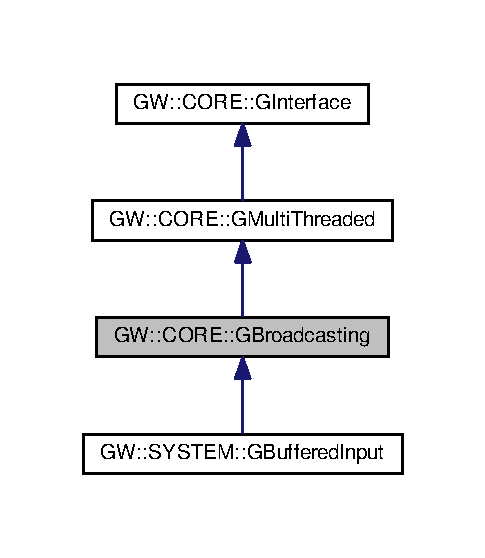
\includegraphics[width=233pt]{classGW_1_1CORE_1_1GBroadcasting__inherit__graph}
\end{center}
\end{figure}


Collaboration diagram for GW\+:\+:C\+O\+RE\+:\+:G\+Broadcasting\+:
\nopagebreak
\begin{figure}[H]
\begin{center}
\leavevmode
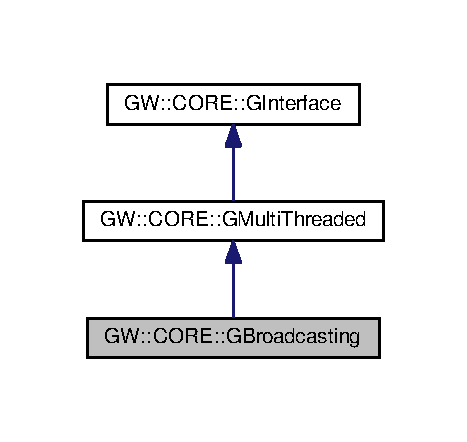
\includegraphics[width=224pt]{classGW_1_1CORE_1_1GBroadcasting__coll__graph}
\end{center}
\end{figure}
\subsection*{Public Member Functions}
\begin{DoxyCompactItemize}
\item 
virtual \hyperlink{namespaceGW_a67a839e3df7ea8a5c5686613a7a3de21}{G\+Return} \hyperlink{classGW_1_1CORE_1_1GBroadcasting_a293251421ba1169016f722df2f5b573b}{Register\+Listener} (\hyperlink{classGW_1_1CORE_1_1GListener}{G\+Listener} $\ast$\+\_\+add\+Listener, unsigned long long \+\_\+event\+Mask)=0
\begin{DoxyCompactList}\small\item\em Any listener added to this class must receive all events unless otherwise specified by the \+\_\+event\+Mask (optional). \end{DoxyCompactList}\item 
virtual \hyperlink{namespaceGW_a67a839e3df7ea8a5c5686613a7a3de21}{G\+Return} \hyperlink{classGW_1_1CORE_1_1GBroadcasting_afd6b1f41b646c668b1fcce2580681dd5}{Deregister\+Listener} (\hyperlink{classGW_1_1CORE_1_1GListener}{G\+Listener} $\ast$\+\_\+remove\+Listener)=0
\begin{DoxyCompactList}\small\item\em A successfully deregistered listener will no longer receive events and have its reference count decremented by one. \end{DoxyCompactList}\end{DoxyCompactItemize}


\subsection{Detailed Description}
The \hyperlink{classGW_1_1CORE_1_1GBroadcasting}{G\+Broadcasting} Interface is capable of registering \& deregistering \hyperlink{classGW_1_1CORE_1_1GListener}{G\+Listener} interfaces. 

The G\+Broadcaster will notify all registered listeners with the listeners On\+Event function. The events being registered for can be filtered with the \+\_\+event\+Mask (optional). 

\subsection{Member Function Documentation}
\index{G\+W\+::\+C\+O\+R\+E\+::\+G\+Broadcasting@{G\+W\+::\+C\+O\+R\+E\+::\+G\+Broadcasting}!Deregister\+Listener@{Deregister\+Listener}}
\index{Deregister\+Listener@{Deregister\+Listener}!G\+W\+::\+C\+O\+R\+E\+::\+G\+Broadcasting@{G\+W\+::\+C\+O\+R\+E\+::\+G\+Broadcasting}}
\subsubsection[{\texorpdfstring{Deregister\+Listener(\+G\+Listener $\ast$\+\_\+remove\+Listener)=0}{DeregisterListener(GListener *_removeListener)=0}}]{\setlength{\rightskip}{0pt plus 5cm}virtual {\bf G\+Return} G\+W\+::\+C\+O\+R\+E\+::\+G\+Broadcasting\+::\+Deregister\+Listener (
\begin{DoxyParamCaption}
\item[{{\bf G\+Listener} $\ast$}]{\+\_\+remove\+Listener}
\end{DoxyParamCaption}
)\hspace{0.3cm}{\ttfamily [pure virtual]}}\hypertarget{classGW_1_1CORE_1_1GBroadcasting_afd6b1f41b646c668b1fcce2580681dd5}{}\label{classGW_1_1CORE_1_1GBroadcasting_afd6b1f41b646c668b1fcce2580681dd5}


A successfully deregistered listener will no longer receive events and have its reference count decremented by one. 


\begin{DoxyParams}[1]{Parameters}
\mbox{\tt in}  & {\em \+\_\+remove\+Listener} & The listener to deregister from events.\\
\hline
\end{DoxyParams}

\begin{DoxyRetVals}{Return values}
{\em S\+U\+C\+C\+E\+SS} & The listener was successfully deregistered. \\
\hline
\end{DoxyRetVals}
\index{G\+W\+::\+C\+O\+R\+E\+::\+G\+Broadcasting@{G\+W\+::\+C\+O\+R\+E\+::\+G\+Broadcasting}!Register\+Listener@{Register\+Listener}}
\index{Register\+Listener@{Register\+Listener}!G\+W\+::\+C\+O\+R\+E\+::\+G\+Broadcasting@{G\+W\+::\+C\+O\+R\+E\+::\+G\+Broadcasting}}
\subsubsection[{\texorpdfstring{Register\+Listener(\+G\+Listener $\ast$\+\_\+add\+Listener, unsigned long long \+\_\+event\+Mask)=0}{RegisterListener(GListener *_addListener, unsigned long long _eventMask)=0}}]{\setlength{\rightskip}{0pt plus 5cm}virtual {\bf G\+Return} G\+W\+::\+C\+O\+R\+E\+::\+G\+Broadcasting\+::\+Register\+Listener (
\begin{DoxyParamCaption}
\item[{{\bf G\+Listener} $\ast$}]{\+\_\+add\+Listener, }
\item[{unsigned long long}]{\+\_\+event\+Mask}
\end{DoxyParamCaption}
)\hspace{0.3cm}{\ttfamily [pure virtual]}}\hypertarget{classGW_1_1CORE_1_1GBroadcasting_a293251421ba1169016f722df2f5b573b}{}\label{classGW_1_1CORE_1_1GBroadcasting_a293251421ba1169016f722df2f5b573b}


Any listener added to this class must receive all events unless otherwise specified by the \+\_\+event\+Mask (optional). 

Listeners registered to a broadcaster will have their reference counts increased by one until deregistered.


\begin{DoxyParams}[1]{Parameters}
\mbox{\tt in}  & {\em \+\_\+add\+Listener} & The listener object that is registering for messages. \\
\hline
\mbox{\tt in}  & {\em \+\_\+event\+Mask} & The events the listener is registering for. 0 will register for all events.\\
\hline
\end{DoxyParams}

\begin{DoxyRetVals}{Return values}
{\em S\+U\+C\+C\+E\+SS} & The listener was successfully registered. \\
\hline
{\em R\+E\+D\+U\+N\+D\+A\+N\+T\+\_\+\+O\+P\+E\+R\+A\+T\+I\+ON} & The listener has already been registered by a previous call. \\
\hline
\end{DoxyRetVals}


The documentation for this class was generated from the following file\+:\begin{DoxyCompactItemize}
\item 
Interface/\+G\+\_\+\+Core/G\+Broadcasting.\+h\end{DoxyCompactItemize}

\hypertarget{classGW_1_1SYSTEM_1_1GBufferedInput}{}\section{GW\+::S\+Y\+S\+T\+EM\+::G\+Buffered\+Input Class Reference}
\label{classGW_1_1SYSTEM_1_1GBufferedInput}\index{GW::SYSTEM::GBufferedInput@{GW::SYSTEM::GBufferedInput}}


A Multi-\/threaded buffered input library.  




{\ttfamily \#include $<$G\+Buffered\+Input.\+h$>$}



Inheritance diagram for GW\+::S\+Y\+S\+T\+EM\+::G\+Buffered\+Input\+:
% FIG 0


Collaboration diagram for GW\+::S\+Y\+S\+T\+EM\+::G\+Buffered\+Input\+:
% FIG 1
\subsection*{Additional Inherited Members}


\subsection{Detailed Description}
A Multi-\/threaded buffered input library. 

Register with a \mbox{\hyperlink{classGW_1_1SYSTEM_1_1GBufferedInput}{G\+Buffered\+Input}} to receive mouse and keyboard events. 

The documentation for this class was generated from the following file\+:\begin{DoxyCompactItemize}
\item 
Interface/\+G\+\_\+\+System/G\+Buffered\+Input.\+h\end{DoxyCompactItemize}

\hypertarget{structGW_1_1SYSTEM_1_1GBUFFEREDINPUT__EVENT__DATA}{}\section{GW\+:\+:S\+Y\+S\+T\+EM\+:\+:G\+B\+U\+F\+F\+E\+R\+E\+D\+I\+N\+P\+U\+T\+\_\+\+E\+V\+E\+N\+T\+\_\+\+D\+A\+TA Struct Reference}
\label{structGW_1_1SYSTEM_1_1GBUFFEREDINPUT__EVENT__DATA}\index{G\+W\+::\+S\+Y\+S\+T\+E\+M\+::\+G\+B\+U\+F\+F\+E\+R\+E\+D\+I\+N\+P\+U\+T\+\_\+\+E\+V\+E\+N\+T\+\_\+\+D\+A\+TA@{G\+W\+::\+S\+Y\+S\+T\+E\+M\+::\+G\+B\+U\+F\+F\+E\+R\+E\+D\+I\+N\+P\+U\+T\+\_\+\+E\+V\+E\+N\+T\+\_\+\+D\+A\+TA}}


Ensure identical binary padding for structures on all platforms.  




{\ttfamily \#include $<$G\+Buffered\+Input.\+h$>$}

\subsection*{Public Attributes}
\begin{DoxyCompactItemize}
\item 
int \hyperlink{structGW_1_1SYSTEM_1_1GBUFFEREDINPUT__EVENT__DATA_abe62d14dd92dc136e8ab4f53ee26d794}{data}
\item 
int \hyperlink{structGW_1_1SYSTEM_1_1GBUFFEREDINPUT__EVENT__DATA_a055e18b0d2aa3135ca8237bb06a0b4cb}{x}
\item 
int \hyperlink{structGW_1_1SYSTEM_1_1GBUFFEREDINPUT__EVENT__DATA_a68facd2e2754c908ecf8b8ef4ce34e08}{y}
\item 
int \hyperlink{structGW_1_1SYSTEM_1_1GBUFFEREDINPUT__EVENT__DATA_a8c87335f76992eddba30abe7312b5b43}{screenX}
\item 
int \hyperlink{structGW_1_1SYSTEM_1_1GBUFFEREDINPUT__EVENT__DATA_a066fa9b2dc654907d13590612238354d}{screenY}
\item 
unsigned int \hyperlink{structGW_1_1SYSTEM_1_1GBUFFEREDINPUT__EVENT__DATA_a7a818ba319e6693b89099938368a699e}{key\+Mask}
\end{DoxyCompactItemize}


\subsection{Detailed Description}
Ensure identical binary padding for structures on all platforms. 

\hyperlink{structGW_1_1SYSTEM_1_1GBUFFEREDINPUT__EVENT__DATA}{G\+B\+U\+F\+F\+E\+R\+E\+D\+I\+N\+P\+U\+T\+\_\+\+E\+V\+E\+N\+T\+\_\+\+D\+A\+TA} will hold any information you may need about an \hyperlink{classInput}{Input} Event. 

\subsection{Member Data Documentation}
\index{G\+W\+::\+S\+Y\+S\+T\+E\+M\+::\+G\+B\+U\+F\+F\+E\+R\+E\+D\+I\+N\+P\+U\+T\+\_\+\+E\+V\+E\+N\+T\+\_\+\+D\+A\+TA@{G\+W\+::\+S\+Y\+S\+T\+E\+M\+::\+G\+B\+U\+F\+F\+E\+R\+E\+D\+I\+N\+P\+U\+T\+\_\+\+E\+V\+E\+N\+T\+\_\+\+D\+A\+TA}!data@{data}}
\index{data@{data}!G\+W\+::\+S\+Y\+S\+T\+E\+M\+::\+G\+B\+U\+F\+F\+E\+R\+E\+D\+I\+N\+P\+U\+T\+\_\+\+E\+V\+E\+N\+T\+\_\+\+D\+A\+TA@{G\+W\+::\+S\+Y\+S\+T\+E\+M\+::\+G\+B\+U\+F\+F\+E\+R\+E\+D\+I\+N\+P\+U\+T\+\_\+\+E\+V\+E\+N\+T\+\_\+\+D\+A\+TA}}
\subsubsection[{\texorpdfstring{data}{data}}]{\setlength{\rightskip}{0pt plus 5cm}int G\+W\+::\+S\+Y\+S\+T\+E\+M\+::\+G\+B\+U\+F\+F\+E\+R\+E\+D\+I\+N\+P\+U\+T\+\_\+\+E\+V\+E\+N\+T\+\_\+\+D\+A\+T\+A\+::data}\hypertarget{structGW_1_1SYSTEM_1_1GBUFFEREDINPUT__EVENT__DATA_abe62d14dd92dc136e8ab4f53ee26d794}{}\label{structGW_1_1SYSTEM_1_1GBUFFEREDINPUT__EVENT__DATA_abe62d14dd92dc136e8ab4f53ee26d794}
Data storing the key/button information. \index{G\+W\+::\+S\+Y\+S\+T\+E\+M\+::\+G\+B\+U\+F\+F\+E\+R\+E\+D\+I\+N\+P\+U\+T\+\_\+\+E\+V\+E\+N\+T\+\_\+\+D\+A\+TA@{G\+W\+::\+S\+Y\+S\+T\+E\+M\+::\+G\+B\+U\+F\+F\+E\+R\+E\+D\+I\+N\+P\+U\+T\+\_\+\+E\+V\+E\+N\+T\+\_\+\+D\+A\+TA}!key\+Mask@{key\+Mask}}
\index{key\+Mask@{key\+Mask}!G\+W\+::\+S\+Y\+S\+T\+E\+M\+::\+G\+B\+U\+F\+F\+E\+R\+E\+D\+I\+N\+P\+U\+T\+\_\+\+E\+V\+E\+N\+T\+\_\+\+D\+A\+TA@{G\+W\+::\+S\+Y\+S\+T\+E\+M\+::\+G\+B\+U\+F\+F\+E\+R\+E\+D\+I\+N\+P\+U\+T\+\_\+\+E\+V\+E\+N\+T\+\_\+\+D\+A\+TA}}
\subsubsection[{\texorpdfstring{key\+Mask}{keyMask}}]{\setlength{\rightskip}{0pt plus 5cm}unsigned int G\+W\+::\+S\+Y\+S\+T\+E\+M\+::\+G\+B\+U\+F\+F\+E\+R\+E\+D\+I\+N\+P\+U\+T\+\_\+\+E\+V\+E\+N\+T\+\_\+\+D\+A\+T\+A\+::key\+Mask}\hypertarget{structGW_1_1SYSTEM_1_1GBUFFEREDINPUT__EVENT__DATA_a7a818ba319e6693b89099938368a699e}{}\label{structGW_1_1SYSTEM_1_1GBUFFEREDINPUT__EVENT__DATA_a7a818ba319e6693b89099938368a699e}
Bit flags for (Caps\+Lock, Num\+Lock, Scroll\+Lock, Shift, and Control). See \hyperlink{GKeyDefines_8h_source}{G\+Key\+Defines.\+h} for list of key\+Mask defines. \index{G\+W\+::\+S\+Y\+S\+T\+E\+M\+::\+G\+B\+U\+F\+F\+E\+R\+E\+D\+I\+N\+P\+U\+T\+\_\+\+E\+V\+E\+N\+T\+\_\+\+D\+A\+TA@{G\+W\+::\+S\+Y\+S\+T\+E\+M\+::\+G\+B\+U\+F\+F\+E\+R\+E\+D\+I\+N\+P\+U\+T\+\_\+\+E\+V\+E\+N\+T\+\_\+\+D\+A\+TA}!screenX@{screenX}}
\index{screenX@{screenX}!G\+W\+::\+S\+Y\+S\+T\+E\+M\+::\+G\+B\+U\+F\+F\+E\+R\+E\+D\+I\+N\+P\+U\+T\+\_\+\+E\+V\+E\+N\+T\+\_\+\+D\+A\+TA@{G\+W\+::\+S\+Y\+S\+T\+E\+M\+::\+G\+B\+U\+F\+F\+E\+R\+E\+D\+I\+N\+P\+U\+T\+\_\+\+E\+V\+E\+N\+T\+\_\+\+D\+A\+TA}}
\subsubsection[{\texorpdfstring{screenX}{screenX}}]{\setlength{\rightskip}{0pt plus 5cm}int G\+W\+::\+S\+Y\+S\+T\+E\+M\+::\+G\+B\+U\+F\+F\+E\+R\+E\+D\+I\+N\+P\+U\+T\+\_\+\+E\+V\+E\+N\+T\+\_\+\+D\+A\+T\+A\+::screenX}\hypertarget{structGW_1_1SYSTEM_1_1GBUFFEREDINPUT__EVENT__DATA_a8c87335f76992eddba30abe7312b5b43}{}\label{structGW_1_1SYSTEM_1_1GBUFFEREDINPUT__EVENT__DATA_a8c87335f76992eddba30abe7312b5b43}
Screen Mouse position x when event is sent. \index{G\+W\+::\+S\+Y\+S\+T\+E\+M\+::\+G\+B\+U\+F\+F\+E\+R\+E\+D\+I\+N\+P\+U\+T\+\_\+\+E\+V\+E\+N\+T\+\_\+\+D\+A\+TA@{G\+W\+::\+S\+Y\+S\+T\+E\+M\+::\+G\+B\+U\+F\+F\+E\+R\+E\+D\+I\+N\+P\+U\+T\+\_\+\+E\+V\+E\+N\+T\+\_\+\+D\+A\+TA}!screenY@{screenY}}
\index{screenY@{screenY}!G\+W\+::\+S\+Y\+S\+T\+E\+M\+::\+G\+B\+U\+F\+F\+E\+R\+E\+D\+I\+N\+P\+U\+T\+\_\+\+E\+V\+E\+N\+T\+\_\+\+D\+A\+TA@{G\+W\+::\+S\+Y\+S\+T\+E\+M\+::\+G\+B\+U\+F\+F\+E\+R\+E\+D\+I\+N\+P\+U\+T\+\_\+\+E\+V\+E\+N\+T\+\_\+\+D\+A\+TA}}
\subsubsection[{\texorpdfstring{screenY}{screenY}}]{\setlength{\rightskip}{0pt plus 5cm}int G\+W\+::\+S\+Y\+S\+T\+E\+M\+::\+G\+B\+U\+F\+F\+E\+R\+E\+D\+I\+N\+P\+U\+T\+\_\+\+E\+V\+E\+N\+T\+\_\+\+D\+A\+T\+A\+::screenY}\hypertarget{structGW_1_1SYSTEM_1_1GBUFFEREDINPUT__EVENT__DATA_a066fa9b2dc654907d13590612238354d}{}\label{structGW_1_1SYSTEM_1_1GBUFFEREDINPUT__EVENT__DATA_a066fa9b2dc654907d13590612238354d}
Screen Mouse position y when event is sent. \index{G\+W\+::\+S\+Y\+S\+T\+E\+M\+::\+G\+B\+U\+F\+F\+E\+R\+E\+D\+I\+N\+P\+U\+T\+\_\+\+E\+V\+E\+N\+T\+\_\+\+D\+A\+TA@{G\+W\+::\+S\+Y\+S\+T\+E\+M\+::\+G\+B\+U\+F\+F\+E\+R\+E\+D\+I\+N\+P\+U\+T\+\_\+\+E\+V\+E\+N\+T\+\_\+\+D\+A\+TA}!x@{x}}
\index{x@{x}!G\+W\+::\+S\+Y\+S\+T\+E\+M\+::\+G\+B\+U\+F\+F\+E\+R\+E\+D\+I\+N\+P\+U\+T\+\_\+\+E\+V\+E\+N\+T\+\_\+\+D\+A\+TA@{G\+W\+::\+S\+Y\+S\+T\+E\+M\+::\+G\+B\+U\+F\+F\+E\+R\+E\+D\+I\+N\+P\+U\+T\+\_\+\+E\+V\+E\+N\+T\+\_\+\+D\+A\+TA}}
\subsubsection[{\texorpdfstring{x}{x}}]{\setlength{\rightskip}{0pt plus 5cm}int G\+W\+::\+S\+Y\+S\+T\+E\+M\+::\+G\+B\+U\+F\+F\+E\+R\+E\+D\+I\+N\+P\+U\+T\+\_\+\+E\+V\+E\+N\+T\+\_\+\+D\+A\+T\+A\+::x}\hypertarget{structGW_1_1SYSTEM_1_1GBUFFEREDINPUT__EVENT__DATA_a055e18b0d2aa3135ca8237bb06a0b4cb}{}\label{structGW_1_1SYSTEM_1_1GBUFFEREDINPUT__EVENT__DATA_a055e18b0d2aa3135ca8237bb06a0b4cb}
Window Mouse position x when event is sent. \index{G\+W\+::\+S\+Y\+S\+T\+E\+M\+::\+G\+B\+U\+F\+F\+E\+R\+E\+D\+I\+N\+P\+U\+T\+\_\+\+E\+V\+E\+N\+T\+\_\+\+D\+A\+TA@{G\+W\+::\+S\+Y\+S\+T\+E\+M\+::\+G\+B\+U\+F\+F\+E\+R\+E\+D\+I\+N\+P\+U\+T\+\_\+\+E\+V\+E\+N\+T\+\_\+\+D\+A\+TA}!y@{y}}
\index{y@{y}!G\+W\+::\+S\+Y\+S\+T\+E\+M\+::\+G\+B\+U\+F\+F\+E\+R\+E\+D\+I\+N\+P\+U\+T\+\_\+\+E\+V\+E\+N\+T\+\_\+\+D\+A\+TA@{G\+W\+::\+S\+Y\+S\+T\+E\+M\+::\+G\+B\+U\+F\+F\+E\+R\+E\+D\+I\+N\+P\+U\+T\+\_\+\+E\+V\+E\+N\+T\+\_\+\+D\+A\+TA}}
\subsubsection[{\texorpdfstring{y}{y}}]{\setlength{\rightskip}{0pt plus 5cm}int G\+W\+::\+S\+Y\+S\+T\+E\+M\+::\+G\+B\+U\+F\+F\+E\+R\+E\+D\+I\+N\+P\+U\+T\+\_\+\+E\+V\+E\+N\+T\+\_\+\+D\+A\+T\+A\+::y}\hypertarget{structGW_1_1SYSTEM_1_1GBUFFEREDINPUT__EVENT__DATA_a68facd2e2754c908ecf8b8ef4ce34e08}{}\label{structGW_1_1SYSTEM_1_1GBUFFEREDINPUT__EVENT__DATA_a68facd2e2754c908ecf8b8ef4ce34e08}
Window Mouse position y when event is sent. 

The documentation for this struct was generated from the following file\+:\begin{DoxyCompactItemize}
\item 
Interface/\+G\+\_\+\+System/G\+Buffered\+Input.\+h\end{DoxyCompactItemize}

\hypertarget{classGW_1_1GRAPHICS_1_1GDirectX11Surface}{}\section{GW\+:\+:G\+R\+A\+P\+H\+I\+CS\+:\+:G\+Direct\+X11\+Surface Class Reference}
\label{classGW_1_1GRAPHICS_1_1GDirectX11Surface}\index{G\+W\+::\+G\+R\+A\+P\+H\+I\+C\+S\+::\+G\+Direct\+X11\+Surface@{G\+W\+::\+G\+R\+A\+P\+H\+I\+C\+S\+::\+G\+Direct\+X11\+Surface}}


A library used to initialize, create, and manage a Direct\+X11 rendering context.  




{\ttfamily \#include $<$G\+Direct\+X11\+Surface.\+h$>$}



Inheritance diagram for GW\+:\+:G\+R\+A\+P\+H\+I\+CS\+:\+:G\+Direct\+X11\+Surface\+:
% FIG 0


Collaboration diagram for GW\+:\+:G\+R\+A\+P\+H\+I\+CS\+:\+:G\+Direct\+X11\+Surface\+:
% FIG 1
\subsection*{Public Member Functions}
\begin{DoxyCompactItemize}
\item 
virtual \mbox{\hyperlink{namespaceGW_a67a839e3df7ea8a5c5686613a7a3de21}{G\+Return}} \mbox{\hyperlink{classGW_1_1GRAPHICS_1_1GDirectX11Surface_a4ae8372993803025a14a8471835ed231}{Get\+Aspect\+Ratio}} (float \&\+\_\+out\+Ratio)=0
\begin{DoxyCompactList}\small\item\em Returns the aspect ratio for the current window. \end{DoxyCompactList}\item 
virtual \mbox{\hyperlink{namespaceGW_a67a839e3df7ea8a5c5686613a7a3de21}{G\+Return}} \mbox{\hyperlink{classGW_1_1GRAPHICS_1_1GDirectX11Surface_a076c4f3a07f79f578185416be449ebd2}{Get\+Device}} (void $\ast$$\ast$\+\_\+out\+Device)=0
\begin{DoxyCompactList}\small\item\em Returns the address of the current I\+D3\+D11\+Device. \end{DoxyCompactList}\item 
virtual \mbox{\hyperlink{namespaceGW_a67a839e3df7ea8a5c5686613a7a3de21}{G\+Return}} \mbox{\hyperlink{classGW_1_1GRAPHICS_1_1GDirectX11Surface_aceaa2e22cbdee6c651cf2045d9320041}{Get\+Context}} (void $\ast$$\ast$\+\_\+out\+Context)=0
\begin{DoxyCompactList}\small\item\em Returns the address of the current I\+D3\+D11\+Device\+Context. \end{DoxyCompactList}\item 
virtual \mbox{\hyperlink{namespaceGW_a67a839e3df7ea8a5c5686613a7a3de21}{G\+Return}} \mbox{\hyperlink{classGW_1_1GRAPHICS_1_1GDirectX11Surface_a8388438c79a82a10f595e10b0bbaab2c}{Get\+Swapchain}} (void $\ast$$\ast$\+\_\+out\+Swapchain)=0
\begin{DoxyCompactList}\small\item\em Returns the address of the current I\+D\+X\+G\+I\+Swap\+Chain. \end{DoxyCompactList}\item 
virtual \mbox{\hyperlink{namespaceGW_a67a839e3df7ea8a5c5686613a7a3de21}{G\+Return}} \mbox{\hyperlink{classGW_1_1GRAPHICS_1_1GDirectX11Surface_a953f4809860408b0e99928ac8b9b6a53}{Get\+Render\+Target}} (void $\ast$$\ast$\+\_\+out\+Render\+Target)=0
\begin{DoxyCompactList}\small\item\em Returns the address of the current I\+D3\+D11\+Render\+Target\+View. \end{DoxyCompactList}\item 
virtual \mbox{\hyperlink{namespaceGW_a67a839e3df7ea8a5c5686613a7a3de21}{G\+Return}} \mbox{\hyperlink{classGW_1_1GRAPHICS_1_1GDirectX11Surface_a44937f7b6e85b0b8df3ac6871c4b87a3}{Get\+Depth\+Stencil\+View}} (void $\ast$$\ast$\+\_\+out\+Depth\+Stencil\+View)=0
\begin{DoxyCompactList}\small\item\em Returns the address of the current I\+D3\+D11\+Depth\+Stencil\+View. \end{DoxyCompactList}\end{DoxyCompactItemize}


\subsection{Detailed Description}
A library used to initialize, create, and manage a Direct\+X11 rendering context. 

This library automates the creation of a basic Direct\+X11 rendering context, and is capable of accepting special requests that can guide the initialization to support requested options. \mbox{\hyperlink{classGW_1_1GRAPHICS_1_1GDirectX11Surface}{G\+Direct\+X11\+Surface}} is a G\+Listener, which allows it to receive events from a registered broadcaster and react accordingly. 

\subsection{Member Function Documentation}
\mbox{\Hypertarget{classGW_1_1GRAPHICS_1_1GDirectX11Surface_a4ae8372993803025a14a8471835ed231}\label{classGW_1_1GRAPHICS_1_1GDirectX11Surface_a4ae8372993803025a14a8471835ed231}} 
\index{G\+W\+::\+G\+R\+A\+P\+H\+I\+C\+S\+::\+G\+Direct\+X11\+Surface@{G\+W\+::\+G\+R\+A\+P\+H\+I\+C\+S\+::\+G\+Direct\+X11\+Surface}!Get\+Aspect\+Ratio@{Get\+Aspect\+Ratio}}
\index{Get\+Aspect\+Ratio@{Get\+Aspect\+Ratio}!G\+W\+::\+G\+R\+A\+P\+H\+I\+C\+S\+::\+G\+Direct\+X11\+Surface@{G\+W\+::\+G\+R\+A\+P\+H\+I\+C\+S\+::\+G\+Direct\+X11\+Surface}}
\subsubsection{\texorpdfstring{Get\+Aspect\+Ratio()}{GetAspectRatio()}}
{\footnotesize\ttfamily virtual \mbox{\hyperlink{namespaceGW_a67a839e3df7ea8a5c5686613a7a3de21}{G\+Return}} G\+W\+::\+G\+R\+A\+P\+H\+I\+C\+S\+::\+G\+Direct\+X11\+Surface\+::\+Get\+Aspect\+Ratio (\begin{DoxyParamCaption}\item[{float \&}]{\+\_\+out\+Ratio }\end{DoxyParamCaption})\hspace{0.3cm}{\ttfamily [pure virtual]}}



Returns the aspect ratio for the current window. 


\begin{DoxyParams}[1]{Parameters}
\mbox{\tt out}  & {\em \+\_\+out\+Ratio} & Will contain the calculated aspect ratio. ~\newline
 \\
\hline
\end{DoxyParams}

\begin{DoxyRetVals}{Return values}
{\em S\+U\+C\+C\+E\+SS} & The current aspect ratio was calculated and returned. \\
\hline
{\em F\+A\+I\+L\+U\+RE} & No active G\+Window exists to calculate an aspect ratio from. \\
\hline
\end{DoxyRetVals}
\mbox{\Hypertarget{classGW_1_1GRAPHICS_1_1GDirectX11Surface_aceaa2e22cbdee6c651cf2045d9320041}\label{classGW_1_1GRAPHICS_1_1GDirectX11Surface_aceaa2e22cbdee6c651cf2045d9320041}} 
\index{G\+W\+::\+G\+R\+A\+P\+H\+I\+C\+S\+::\+G\+Direct\+X11\+Surface@{G\+W\+::\+G\+R\+A\+P\+H\+I\+C\+S\+::\+G\+Direct\+X11\+Surface}!Get\+Context@{Get\+Context}}
\index{Get\+Context@{Get\+Context}!G\+W\+::\+G\+R\+A\+P\+H\+I\+C\+S\+::\+G\+Direct\+X11\+Surface@{G\+W\+::\+G\+R\+A\+P\+H\+I\+C\+S\+::\+G\+Direct\+X11\+Surface}}
\subsubsection{\texorpdfstring{Get\+Context()}{GetContext()}}
{\footnotesize\ttfamily virtual \mbox{\hyperlink{namespaceGW_a67a839e3df7ea8a5c5686613a7a3de21}{G\+Return}} G\+W\+::\+G\+R\+A\+P\+H\+I\+C\+S\+::\+G\+Direct\+X11\+Surface\+::\+Get\+Context (\begin{DoxyParamCaption}\item[{void $\ast$$\ast$}]{\+\_\+out\+Context }\end{DoxyParamCaption})\hspace{0.3cm}{\ttfamily [pure virtual]}}



Returns the address of the current I\+D3\+D11\+Device\+Context. 


\begin{DoxyParams}[1]{Parameters}
\mbox{\tt out}  & {\em \+\_\+out\+Context} & Will contain the address of the context.\\
\hline
\end{DoxyParams}

\begin{DoxyRetVals}{Return values}
{\em S\+U\+C\+C\+E\+SS} & A Direct\+X11 contexts exists and was returned. \\
\hline
{\em F\+A\+I\+L\+U\+RE} & No context exists to retrieve. \\
\hline
\end{DoxyRetVals}
\mbox{\Hypertarget{classGW_1_1GRAPHICS_1_1GDirectX11Surface_a44937f7b6e85b0b8df3ac6871c4b87a3}\label{classGW_1_1GRAPHICS_1_1GDirectX11Surface_a44937f7b6e85b0b8df3ac6871c4b87a3}} 
\index{G\+W\+::\+G\+R\+A\+P\+H\+I\+C\+S\+::\+G\+Direct\+X11\+Surface@{G\+W\+::\+G\+R\+A\+P\+H\+I\+C\+S\+::\+G\+Direct\+X11\+Surface}!Get\+Depth\+Stencil\+View@{Get\+Depth\+Stencil\+View}}
\index{Get\+Depth\+Stencil\+View@{Get\+Depth\+Stencil\+View}!G\+W\+::\+G\+R\+A\+P\+H\+I\+C\+S\+::\+G\+Direct\+X11\+Surface@{G\+W\+::\+G\+R\+A\+P\+H\+I\+C\+S\+::\+G\+Direct\+X11\+Surface}}
\subsubsection{\texorpdfstring{Get\+Depth\+Stencil\+View()}{GetDepthStencilView()}}
{\footnotesize\ttfamily virtual \mbox{\hyperlink{namespaceGW_a67a839e3df7ea8a5c5686613a7a3de21}{G\+Return}} G\+W\+::\+G\+R\+A\+P\+H\+I\+C\+S\+::\+G\+Direct\+X11\+Surface\+::\+Get\+Depth\+Stencil\+View (\begin{DoxyParamCaption}\item[{void $\ast$$\ast$}]{\+\_\+out\+Depth\+Stencil\+View }\end{DoxyParamCaption})\hspace{0.3cm}{\ttfamily [pure virtual]}}



Returns the address of the current I\+D3\+D11\+Depth\+Stencil\+View. 

A Depth Stencil View will only be created if requested as a special option when the \textquotesingle{}Initialize\textquotesingle{} method is called.


\begin{DoxyParams}[1]{Parameters}
\mbox{\tt out}  & {\em \+\_\+out\+Depth\+Stencil\+View} & Will contain the address of the depth stencil view.\\
\hline
\end{DoxyParams}

\begin{DoxyRetVals}{Return values}
{\em S\+U\+C\+C\+E\+SS} & A Direct\+X11 depth stencil view exists and was returned. \\
\hline
{\em F\+A\+I\+L\+U\+RE} & No depth stencil view exists to retrieve. \\
\hline
\end{DoxyRetVals}
\mbox{\Hypertarget{classGW_1_1GRAPHICS_1_1GDirectX11Surface_a076c4f3a07f79f578185416be449ebd2}\label{classGW_1_1GRAPHICS_1_1GDirectX11Surface_a076c4f3a07f79f578185416be449ebd2}} 
\index{G\+W\+::\+G\+R\+A\+P\+H\+I\+C\+S\+::\+G\+Direct\+X11\+Surface@{G\+W\+::\+G\+R\+A\+P\+H\+I\+C\+S\+::\+G\+Direct\+X11\+Surface}!Get\+Device@{Get\+Device}}
\index{Get\+Device@{Get\+Device}!G\+W\+::\+G\+R\+A\+P\+H\+I\+C\+S\+::\+G\+Direct\+X11\+Surface@{G\+W\+::\+G\+R\+A\+P\+H\+I\+C\+S\+::\+G\+Direct\+X11\+Surface}}
\subsubsection{\texorpdfstring{Get\+Device()}{GetDevice()}}
{\footnotesize\ttfamily virtual \mbox{\hyperlink{namespaceGW_a67a839e3df7ea8a5c5686613a7a3de21}{G\+Return}} G\+W\+::\+G\+R\+A\+P\+H\+I\+C\+S\+::\+G\+Direct\+X11\+Surface\+::\+Get\+Device (\begin{DoxyParamCaption}\item[{void $\ast$$\ast$}]{\+\_\+out\+Device }\end{DoxyParamCaption})\hspace{0.3cm}{\ttfamily [pure virtual]}}



Returns the address of the current I\+D3\+D11\+Device. 


\begin{DoxyParams}[1]{Parameters}
\mbox{\tt out}  & {\em \+\_\+out\+Device} & Will contain the address of the device.\\
\hline
\end{DoxyParams}

\begin{DoxyRetVals}{Return values}
{\em S\+U\+C\+C\+E\+SS} & A Direct\+X11 device exists and was returned. \\
\hline
{\em F\+A\+I\+L\+U\+RE} & No device exists to retrieve. \\
\hline
\end{DoxyRetVals}
\mbox{\Hypertarget{classGW_1_1GRAPHICS_1_1GDirectX11Surface_a953f4809860408b0e99928ac8b9b6a53}\label{classGW_1_1GRAPHICS_1_1GDirectX11Surface_a953f4809860408b0e99928ac8b9b6a53}} 
\index{G\+W\+::\+G\+R\+A\+P\+H\+I\+C\+S\+::\+G\+Direct\+X11\+Surface@{G\+W\+::\+G\+R\+A\+P\+H\+I\+C\+S\+::\+G\+Direct\+X11\+Surface}!Get\+Render\+Target@{Get\+Render\+Target}}
\index{Get\+Render\+Target@{Get\+Render\+Target}!G\+W\+::\+G\+R\+A\+P\+H\+I\+C\+S\+::\+G\+Direct\+X11\+Surface@{G\+W\+::\+G\+R\+A\+P\+H\+I\+C\+S\+::\+G\+Direct\+X11\+Surface}}
\subsubsection{\texorpdfstring{Get\+Render\+Target()}{GetRenderTarget()}}
{\footnotesize\ttfamily virtual \mbox{\hyperlink{namespaceGW_a67a839e3df7ea8a5c5686613a7a3de21}{G\+Return}} G\+W\+::\+G\+R\+A\+P\+H\+I\+C\+S\+::\+G\+Direct\+X11\+Surface\+::\+Get\+Render\+Target (\begin{DoxyParamCaption}\item[{void $\ast$$\ast$}]{\+\_\+out\+Render\+Target }\end{DoxyParamCaption})\hspace{0.3cm}{\ttfamily [pure virtual]}}



Returns the address of the current I\+D3\+D11\+Render\+Target\+View. 


\begin{DoxyParams}[1]{Parameters}
\mbox{\tt out}  & {\em \+\_\+out\+Render\+Target} & Will contain the address of the render target view.\\
\hline
\end{DoxyParams}

\begin{DoxyRetVals}{Return values}
{\em S\+U\+C\+C\+E\+SS} & A Direct\+X11 render target view exists and was returned. \\
\hline
{\em F\+A\+I\+L\+U\+RE} & No render target view exists to retrieve. \\
\hline
\end{DoxyRetVals}
\mbox{\Hypertarget{classGW_1_1GRAPHICS_1_1GDirectX11Surface_a8388438c79a82a10f595e10b0bbaab2c}\label{classGW_1_1GRAPHICS_1_1GDirectX11Surface_a8388438c79a82a10f595e10b0bbaab2c}} 
\index{G\+W\+::\+G\+R\+A\+P\+H\+I\+C\+S\+::\+G\+Direct\+X11\+Surface@{G\+W\+::\+G\+R\+A\+P\+H\+I\+C\+S\+::\+G\+Direct\+X11\+Surface}!Get\+Swapchain@{Get\+Swapchain}}
\index{Get\+Swapchain@{Get\+Swapchain}!G\+W\+::\+G\+R\+A\+P\+H\+I\+C\+S\+::\+G\+Direct\+X11\+Surface@{G\+W\+::\+G\+R\+A\+P\+H\+I\+C\+S\+::\+G\+Direct\+X11\+Surface}}
\subsubsection{\texorpdfstring{Get\+Swapchain()}{GetSwapchain()}}
{\footnotesize\ttfamily virtual \mbox{\hyperlink{namespaceGW_a67a839e3df7ea8a5c5686613a7a3de21}{G\+Return}} G\+W\+::\+G\+R\+A\+P\+H\+I\+C\+S\+::\+G\+Direct\+X11\+Surface\+::\+Get\+Swapchain (\begin{DoxyParamCaption}\item[{void $\ast$$\ast$}]{\+\_\+out\+Swapchain }\end{DoxyParamCaption})\hspace{0.3cm}{\ttfamily [pure virtual]}}



Returns the address of the current I\+D\+X\+G\+I\+Swap\+Chain. 


\begin{DoxyParams}[1]{Parameters}
\mbox{\tt out}  & {\em \+\_\+out\+Swapchain} & Will contain the address of the swap chain.\\
\hline
\end{DoxyParams}

\begin{DoxyRetVals}{Return values}
{\em S\+U\+C\+C\+E\+SS} & A Direct\+X11 swap chain exists and was returned. \\
\hline
{\em F\+A\+I\+L\+U\+RE} & No swap chain exists to retrieve. \\
\hline
\end{DoxyRetVals}


The documentation for this class was generated from the following file\+:\begin{DoxyCompactItemize}
\item 
Interface/\+G\+\_\+\+Graphics/G\+Direct\+X11\+Surface.\+h\end{DoxyCompactItemize}

\hypertarget{classGW_1_1SYSTEM_1_1GFile}{}\section{GW\+:\+:S\+Y\+S\+T\+EM\+:\+:G\+File Class Reference}
\label{classGW_1_1SYSTEM_1_1GFile}\index{G\+W\+::\+S\+Y\+S\+T\+E\+M\+::\+G\+File@{G\+W\+::\+S\+Y\+S\+T\+E\+M\+::\+G\+File}}


Cross platform File\+I\+O/\+Directory handling.  




{\ttfamily \#include $<$G\+File.\+h$>$}



Inheritance diagram for GW\+:\+:S\+Y\+S\+T\+EM\+:\+:G\+File\+:
\nopagebreak
\begin{figure}[H]
\begin{center}
\leavevmode
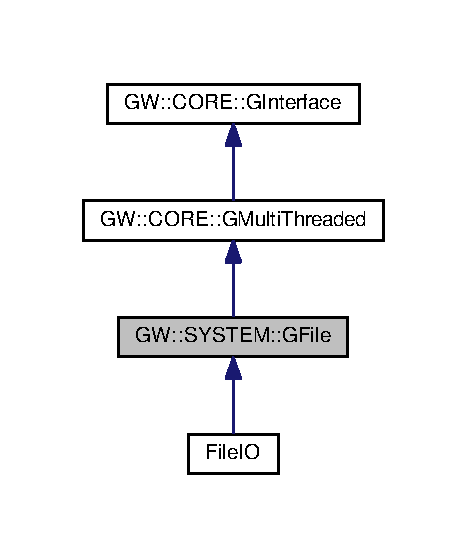
\includegraphics[width=224pt]{classGW_1_1SYSTEM_1_1GFile__inherit__graph}
\end{center}
\end{figure}


Collaboration diagram for GW\+:\+:S\+Y\+S\+T\+EM\+:\+:G\+File\+:
\nopagebreak
\begin{figure}[H]
\begin{center}
\leavevmode
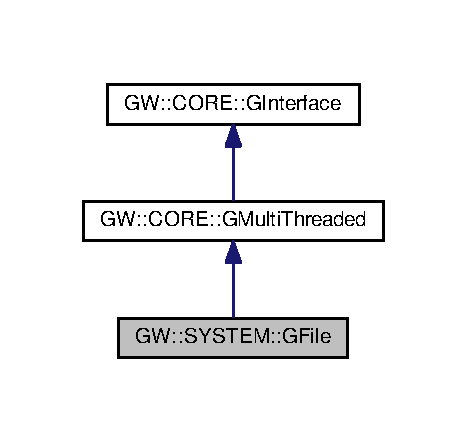
\includegraphics[width=224pt]{classGW_1_1SYSTEM_1_1GFile__coll__graph}
\end{center}
\end{figure}
\subsection*{Public Member Functions}
\begin{DoxyCompactItemize}
\item 
virtual \hyperlink{namespaceGW_a67a839e3df7ea8a5c5686613a7a3de21}{G\+Return} \hyperlink{classGW_1_1SYSTEM_1_1GFile_a2744359d5d258b1b59d139101c6809ce}{Open\+Binary\+Read} (const char $\ast$const \+\_\+file)=0
\begin{DoxyCompactList}\small\item\em Opens a file for binary read. \end{DoxyCompactList}\item 
virtual \hyperlink{namespaceGW_a67a839e3df7ea8a5c5686613a7a3de21}{G\+Return} \hyperlink{classGW_1_1SYSTEM_1_1GFile_a8d5f335bbc6f7c6d798ed27718aa2347}{Open\+Binary\+Write} (const char $\ast$const \+\_\+file)=0
\begin{DoxyCompactList}\small\item\em Opens a file for binary write with truncation. \end{DoxyCompactList}\item 
virtual \hyperlink{namespaceGW_a67a839e3df7ea8a5c5686613a7a3de21}{G\+Return} \hyperlink{classGW_1_1SYSTEM_1_1GFile_a63311236692181f99fd393fe8e1ca9fc}{Append\+Binary\+Write} (const char $\ast$const \+\_\+file)=0
\begin{DoxyCompactList}\small\item\em Opens a file for binary write with append. \end{DoxyCompactList}\item 
virtual \hyperlink{namespaceGW_a67a839e3df7ea8a5c5686613a7a3de21}{G\+Return} \hyperlink{classGW_1_1SYSTEM_1_1GFile_ac3ece72ce30e4d1a1c426c53a7a8354a}{Open\+Text\+Read} (const char $\ast$const \+\_\+file)=0
\begin{DoxyCompactList}\small\item\em Opens a file for text read. \end{DoxyCompactList}\item 
virtual \hyperlink{namespaceGW_a67a839e3df7ea8a5c5686613a7a3de21}{G\+Return} \hyperlink{classGW_1_1SYSTEM_1_1GFile_aebd3e32736b994c0296b7575ab0a2759}{Open\+Text\+Write} (const char $\ast$const \+\_\+file)=0
\begin{DoxyCompactList}\small\item\em Opens a file for text write with truncation. \end{DoxyCompactList}\item 
virtual \hyperlink{namespaceGW_a67a839e3df7ea8a5c5686613a7a3de21}{G\+Return} \hyperlink{classGW_1_1SYSTEM_1_1GFile_a72e40b3234a2384738d8db6e958f4782}{Append\+Text\+Write} (const char $\ast$const \+\_\+file)=0
\begin{DoxyCompactList}\small\item\em Opens a file for text write with append. \end{DoxyCompactList}\item 
virtual \hyperlink{namespaceGW_a67a839e3df7ea8a5c5686613a7a3de21}{G\+Return} \hyperlink{classGW_1_1SYSTEM_1_1GFile_ae9906414c159e9f1156b5ff6ad511c31}{Write} (const char $\ast$const \+\_\+in\+Data, unsigned int \+\_\+num\+Bytes)=0
\begin{DoxyCompactList}\small\item\em Writes binary data to the currently opened file. \end{DoxyCompactList}\item 
virtual \hyperlink{namespaceGW_a67a839e3df7ea8a5c5686613a7a3de21}{G\+Return} \hyperlink{classGW_1_1SYSTEM_1_1GFile_a1aaa026cba3d37abaaa2b408cd5d322d}{Read} (char $\ast$\+\_\+out\+Data, unsigned int \+\_\+num\+Bytes)=0
\begin{DoxyCompactList}\small\item\em Reads binary from the currently opened file. \end{DoxyCompactList}\item 
virtual \hyperlink{namespaceGW_a67a839e3df7ea8a5c5686613a7a3de21}{G\+Return} \hyperlink{classGW_1_1SYSTEM_1_1GFile_a7c57570575c63ae98f71232660d1b911}{Write\+Line} (const char $\ast$const \+\_\+in\+Data)=0
\begin{DoxyCompactList}\small\item\em Writes text to the currently opened file. \end{DoxyCompactList}\item 
virtual \hyperlink{namespaceGW_a67a839e3df7ea8a5c5686613a7a3de21}{G\+Return} \hyperlink{classGW_1_1SYSTEM_1_1GFile_ae9e072091ffe55f2f7697cb1d3eaec79}{Read\+Line} (char $\ast$\+\_\+out\+Data, unsigned int \+\_\+out\+Data\+Size, char \+\_\+delimiter)=0
\begin{DoxyCompactList}\small\item\em Reads text to the currently opened file. \end{DoxyCompactList}\item 
virtual \hyperlink{namespaceGW_a67a839e3df7ea8a5c5686613a7a3de21}{G\+Return} \hyperlink{classGW_1_1SYSTEM_1_1GFile_ae661d107c461145bb095dcfc76519f54}{Close\+File} ()=0
\begin{DoxyCompactList}\small\item\em Flushes and closes the current file. \end{DoxyCompactList}\item 
virtual \hyperlink{namespaceGW_a67a839e3df7ea8a5c5686613a7a3de21}{G\+Return} \hyperlink{classGW_1_1SYSTEM_1_1GFile_ae3105b637ef87af268722a696b8657a9}{Flush\+File} ()=0
\begin{DoxyCompactList}\small\item\em Flushes the current file. \end{DoxyCompactList}\item 
virtual \hyperlink{namespaceGW_a67a839e3df7ea8a5c5686613a7a3de21}{G\+Return} \hyperlink{classGW_1_1SYSTEM_1_1GFile_ab28d2e7ecf3ac893df88603e5448561a}{Set\+Current\+Working\+Directory} (const char $\ast$const \+\_\+dir)=0
\begin{DoxyCompactList}\small\item\em Changes the current working directory. \end{DoxyCompactList}\item 
virtual \hyperlink{namespaceGW_a67a839e3df7ea8a5c5686613a7a3de21}{G\+Return} \hyperlink{classGW_1_1SYSTEM_1_1GFile_a6853b717e838d1b3a54f22449a37d764}{Get\+Current\+Working\+Directory} (char $\ast$\+\_\+out\+Dir, unsigned int \+\_\+dir\+Size)=0
\begin{DoxyCompactList}\small\item\em Retrieves the absolute path of the current working directory. \end{DoxyCompactList}\item 
virtual \hyperlink{namespaceGW_a67a839e3df7ea8a5c5686613a7a3de21}{G\+Return} \hyperlink{classGW_1_1SYSTEM_1_1GFile_ac2de86bf6cf61455577efc47277ecb94}{Get\+Directory\+Size} (unsigned int \&\+\_\+out\+Size)=0
\begin{DoxyCompactList}\small\item\em Gets the number of files in the current working directory. \end{DoxyCompactList}\item 
virtual \hyperlink{namespaceGW_a67a839e3df7ea8a5c5686613a7a3de21}{G\+Return} \hyperlink{classGW_1_1SYSTEM_1_1GFile_ae062d19f84d120adea94756d1d26e41e}{Get\+Files\+From\+Directory} (char $\ast$\+\_\+out\+Files\mbox{[}$\,$\mbox{]}, unsigned int \+\_\+num\+Files, unsigned int \+\_\+file\+Name\+Size)=0
\begin{DoxyCompactList}\small\item\em Gets the names of all files in the current working directory. \end{DoxyCompactList}\item 
virtual \hyperlink{namespaceGW_a67a839e3df7ea8a5c5686613a7a3de21}{G\+Return} \hyperlink{classGW_1_1SYSTEM_1_1GFile_a2f4cba2dad96fa4c894545f43fee64b5}{Get\+File\+Size} (const char $\ast$const \+\_\+file, unsigned int \&\+\_\+out\+Size)=0
\begin{DoxyCompactList}\small\item\em Gets the size of the specified file in bytes. \end{DoxyCompactList}\end{DoxyCompactItemize}


\subsection{Detailed Description}
Cross platform File\+I\+O/\+Directory handling. 

Handles file input/output operations, as well as directory information and file information. Inherits from G\+Multi\+Threaded, therfore its implementation must be thread safe. 

\subsection{Member Function Documentation}
\index{G\+W\+::\+S\+Y\+S\+T\+E\+M\+::\+G\+File@{G\+W\+::\+S\+Y\+S\+T\+E\+M\+::\+G\+File}!Append\+Binary\+Write@{Append\+Binary\+Write}}
\index{Append\+Binary\+Write@{Append\+Binary\+Write}!G\+W\+::\+S\+Y\+S\+T\+E\+M\+::\+G\+File@{G\+W\+::\+S\+Y\+S\+T\+E\+M\+::\+G\+File}}
\subsubsection[{\texorpdfstring{Append\+Binary\+Write(const char $\ast$const \+\_\+file)=0}{AppendBinaryWrite(const char *const _file)=0}}]{\setlength{\rightskip}{0pt plus 5cm}virtual {\bf G\+Return} G\+W\+::\+S\+Y\+S\+T\+E\+M\+::\+G\+File\+::\+Append\+Binary\+Write (
\begin{DoxyParamCaption}
\item[{const char $\ast$const}]{\+\_\+file}
\end{DoxyParamCaption}
)\hspace{0.3cm}{\ttfamily [pure virtual]}}\hypertarget{classGW_1_1SYSTEM_1_1GFile_a63311236692181f99fd393fe8e1ca9fc}{}\label{classGW_1_1SYSTEM_1_1GFile_a63311236692181f99fd393fe8e1ca9fc}


Opens a file for binary write with append. 

The file name passed into the function should be passed like it is a relative path. The function will look in the current working directory for the file. If the file is not found in the current working directory, the file will be created in the current working directory. File can now be written to with \hyperlink{classGW_1_1SYSTEM_1_1GFile_ae9906414c159e9f1156b5ff6ad511c31}{Write()}.


\begin{DoxyParams}[1]{Parameters}
\mbox{\tt in}  & {\em \+\_\+file} & The file name of the file to open.\\
\hline
\end{DoxyParams}

\begin{DoxyRetVals}{Return values}
{\em S\+U\+C\+C\+E\+SS} & Succesfully opened the file. \\
\hline
{\em F\+A\+I\+L\+U\+RE} & A file is already open or the file could not be found/created. \\
\hline
{\em I\+N\+V\+A\+L\+I\+D\+\_\+\+A\+R\+G\+U\+M\+E\+NT} & A nullptr was passed in. \\
\hline
\end{DoxyRetVals}


Implemented in \hyperlink{classFileIO_ab26fc846b30446edf28ac922759c9e5e}{File\+IO}.

\index{G\+W\+::\+S\+Y\+S\+T\+E\+M\+::\+G\+File@{G\+W\+::\+S\+Y\+S\+T\+E\+M\+::\+G\+File}!Append\+Text\+Write@{Append\+Text\+Write}}
\index{Append\+Text\+Write@{Append\+Text\+Write}!G\+W\+::\+S\+Y\+S\+T\+E\+M\+::\+G\+File@{G\+W\+::\+S\+Y\+S\+T\+E\+M\+::\+G\+File}}
\subsubsection[{\texorpdfstring{Append\+Text\+Write(const char $\ast$const \+\_\+file)=0}{AppendTextWrite(const char *const _file)=0}}]{\setlength{\rightskip}{0pt plus 5cm}virtual {\bf G\+Return} G\+W\+::\+S\+Y\+S\+T\+E\+M\+::\+G\+File\+::\+Append\+Text\+Write (
\begin{DoxyParamCaption}
\item[{const char $\ast$const}]{\+\_\+file}
\end{DoxyParamCaption}
)\hspace{0.3cm}{\ttfamily [pure virtual]}}\hypertarget{classGW_1_1SYSTEM_1_1GFile_a72e40b3234a2384738d8db6e958f4782}{}\label{classGW_1_1SYSTEM_1_1GFile_a72e40b3234a2384738d8db6e958f4782}


Opens a file for text write with append. 

The file name passed into the function should be passed like it is a relative path. The function will look in the current working directory for the file. If the file is not found in the current working directory, the file will be created in the current working directory. File can now be written to with \hyperlink{classGW_1_1SYSTEM_1_1GFile_ae9906414c159e9f1156b5ff6ad511c31}{Write()}.


\begin{DoxyParams}[1]{Parameters}
\mbox{\tt in}  & {\em \+\_\+file} & The file name of the file to open.\\
\hline
\end{DoxyParams}

\begin{DoxyRetVals}{Return values}
{\em S\+U\+C\+C\+E\+SS} & Succesfully opened the file. \\
\hline
{\em F\+A\+I\+L\+U\+RE} & A file is already open or the file could not be found/created. \\
\hline
{\em I\+N\+V\+A\+L\+I\+D\+\_\+\+A\+R\+G\+U\+M\+E\+NT} & A nullptr was passed in. \\
\hline
\end{DoxyRetVals}


Implemented in \hyperlink{classFileIO_afd4e0d14b85d8c0aded66bd946c291f4}{File\+IO}.

\index{G\+W\+::\+S\+Y\+S\+T\+E\+M\+::\+G\+File@{G\+W\+::\+S\+Y\+S\+T\+E\+M\+::\+G\+File}!Close\+File@{Close\+File}}
\index{Close\+File@{Close\+File}!G\+W\+::\+S\+Y\+S\+T\+E\+M\+::\+G\+File@{G\+W\+::\+S\+Y\+S\+T\+E\+M\+::\+G\+File}}
\subsubsection[{\texorpdfstring{Close\+File()=0}{CloseFile()=0}}]{\setlength{\rightskip}{0pt plus 5cm}virtual {\bf G\+Return} G\+W\+::\+S\+Y\+S\+T\+E\+M\+::\+G\+File\+::\+Close\+File (
\begin{DoxyParamCaption}
{}
\end{DoxyParamCaption}
)\hspace{0.3cm}{\ttfamily [pure virtual]}}\hypertarget{classGW_1_1SYSTEM_1_1GFile_ae661d107c461145bb095dcfc76519f54}{}\label{classGW_1_1SYSTEM_1_1GFile_ae661d107c461145bb095dcfc76519f54}


Flushes and closes the current file. 


\begin{DoxyRetVals}{Return values}
{\em S\+U\+C\+C\+E\+SS} & File successfully flushed and closed. \\
\hline
{\em F\+A\+I\+L\+U\+RE} & A file is not currently open. \\
\hline
\end{DoxyRetVals}


Implemented in \hyperlink{classFileIO_a906610c8653ba8ca476dc46679851590}{File\+IO}.

\index{G\+W\+::\+S\+Y\+S\+T\+E\+M\+::\+G\+File@{G\+W\+::\+S\+Y\+S\+T\+E\+M\+::\+G\+File}!Flush\+File@{Flush\+File}}
\index{Flush\+File@{Flush\+File}!G\+W\+::\+S\+Y\+S\+T\+E\+M\+::\+G\+File@{G\+W\+::\+S\+Y\+S\+T\+E\+M\+::\+G\+File}}
\subsubsection[{\texorpdfstring{Flush\+File()=0}{FlushFile()=0}}]{\setlength{\rightskip}{0pt plus 5cm}virtual {\bf G\+Return} G\+W\+::\+S\+Y\+S\+T\+E\+M\+::\+G\+File\+::\+Flush\+File (
\begin{DoxyParamCaption}
{}
\end{DoxyParamCaption}
)\hspace{0.3cm}{\ttfamily [pure virtual]}}\hypertarget{classGW_1_1SYSTEM_1_1GFile_ae3105b637ef87af268722a696b8657a9}{}\label{classGW_1_1SYSTEM_1_1GFile_ae3105b637ef87af268722a696b8657a9}


Flushes the current file. 


\begin{DoxyRetVals}{Return values}
{\em S\+U\+C\+C\+E\+SS} & File successfully flushed. \\
\hline
{\em F\+A\+I\+L\+U\+RE} & A file is not currently open. \\
\hline
\end{DoxyRetVals}


Implemented in \hyperlink{classFileIO_a8e5afdb1a734f37e422ff0147561a3a1}{File\+IO}.

\index{G\+W\+::\+S\+Y\+S\+T\+E\+M\+::\+G\+File@{G\+W\+::\+S\+Y\+S\+T\+E\+M\+::\+G\+File}!Get\+Current\+Working\+Directory@{Get\+Current\+Working\+Directory}}
\index{Get\+Current\+Working\+Directory@{Get\+Current\+Working\+Directory}!G\+W\+::\+S\+Y\+S\+T\+E\+M\+::\+G\+File@{G\+W\+::\+S\+Y\+S\+T\+E\+M\+::\+G\+File}}
\subsubsection[{\texorpdfstring{Get\+Current\+Working\+Directory(char $\ast$\+\_\+out\+Dir, unsigned int \+\_\+dir\+Size)=0}{GetCurrentWorkingDirectory(char *_outDir, unsigned int _dirSize)=0}}]{\setlength{\rightskip}{0pt plus 5cm}virtual {\bf G\+Return} G\+W\+::\+S\+Y\+S\+T\+E\+M\+::\+G\+File\+::\+Get\+Current\+Working\+Directory (
\begin{DoxyParamCaption}
\item[{char $\ast$}]{\+\_\+out\+Dir, }
\item[{unsigned int}]{\+\_\+dir\+Size}
\end{DoxyParamCaption}
)\hspace{0.3cm}{\ttfamily [pure virtual]}}\hypertarget{classGW_1_1SYSTEM_1_1GFile_a6853b717e838d1b3a54f22449a37d764}{}\label{classGW_1_1SYSTEM_1_1GFile_a6853b717e838d1b3a54f22449a37d764}


Retrieves the absolute path of the current working directory. 

This is the directory we will look into for any file Open commands. This is by Windows standard guaranteed to be 255 or less.


\begin{DoxyParams}[1]{Parameters}
\mbox{\tt out}  & {\em \+\_\+out\+Dir} & An absolute path to the directory to set as the current working directory. \\
\hline
\mbox{\tt in}  & {\em \+\_\+dir\+Size} & The size of \+\_\+out\+Dir.\\
\hline
\end{DoxyParams}

\begin{DoxyRetVals}{Return values}
{\em S\+U\+C\+C\+E\+SS} & Successfully obtained the working directory. \\
\hline
{\em F\+A\+I\+L\+U\+RE} & The current working directory is invalid or \+\_\+out\+Dir was not big enough. \+\_\+out\+Dir will be null. \\
\hline
{\em I\+N\+V\+A\+L\+I\+D\+\_\+\+A\+R\+G\+U\+M\+E\+NT} & A nullptr was passed in or the size is 0. \\
\hline
\end{DoxyRetVals}


Implemented in \hyperlink{classFileIO_a41a1859ffe3ebd76005f264af0b1ea66}{File\+IO}.

\index{G\+W\+::\+S\+Y\+S\+T\+E\+M\+::\+G\+File@{G\+W\+::\+S\+Y\+S\+T\+E\+M\+::\+G\+File}!Get\+Directory\+Size@{Get\+Directory\+Size}}
\index{Get\+Directory\+Size@{Get\+Directory\+Size}!G\+W\+::\+S\+Y\+S\+T\+E\+M\+::\+G\+File@{G\+W\+::\+S\+Y\+S\+T\+E\+M\+::\+G\+File}}
\subsubsection[{\texorpdfstring{Get\+Directory\+Size(unsigned int \&\+\_\+out\+Size)=0}{GetDirectorySize(unsigned int &_outSize)=0}}]{\setlength{\rightskip}{0pt plus 5cm}virtual {\bf G\+Return} G\+W\+::\+S\+Y\+S\+T\+E\+M\+::\+G\+File\+::\+Get\+Directory\+Size (
\begin{DoxyParamCaption}
\item[{unsigned int \&}]{\+\_\+out\+Size}
\end{DoxyParamCaption}
)\hspace{0.3cm}{\ttfamily [pure virtual]}}\hypertarget{classGW_1_1SYSTEM_1_1GFile_ac2de86bf6cf61455577efc47277ecb94}{}\label{classGW_1_1SYSTEM_1_1GFile_ac2de86bf6cf61455577efc47277ecb94}


Gets the number of files in the current working directory. 


\begin{DoxyParams}[1]{Parameters}
\mbox{\tt out}  & {\em \+\_\+out\+Size} & The number of files in the directory.\\
\hline
\end{DoxyParams}

\begin{DoxyRetVals}{Return values}
{\em S\+U\+C\+C\+E\+SS} & Successfully counted the files in the directory. \\
\hline
{\em F\+A\+I\+L\+U\+RE} & Either currently working directory is invalid or count failed. \+\_\+out\+Size will be -\/1. \\
\hline
\end{DoxyRetVals}


Implemented in \hyperlink{classFileIO_ae331f6c02948720d9cc5bcd2700d8cf7}{File\+IO}.

\index{G\+W\+::\+S\+Y\+S\+T\+E\+M\+::\+G\+File@{G\+W\+::\+S\+Y\+S\+T\+E\+M\+::\+G\+File}!Get\+Files\+From\+Directory@{Get\+Files\+From\+Directory}}
\index{Get\+Files\+From\+Directory@{Get\+Files\+From\+Directory}!G\+W\+::\+S\+Y\+S\+T\+E\+M\+::\+G\+File@{G\+W\+::\+S\+Y\+S\+T\+E\+M\+::\+G\+File}}
\subsubsection[{\texorpdfstring{Get\+Files\+From\+Directory(char $\ast$\+\_\+out\+Files[], unsigned int \+\_\+num\+Files, unsigned int \+\_\+file\+Name\+Size)=0}{GetFilesFromDirectory(char *_outFiles[], unsigned int _numFiles, unsigned int _fileNameSize)=0}}]{\setlength{\rightskip}{0pt plus 5cm}virtual {\bf G\+Return} G\+W\+::\+S\+Y\+S\+T\+E\+M\+::\+G\+File\+::\+Get\+Files\+From\+Directory (
\begin{DoxyParamCaption}
\item[{char $\ast$}]{\+\_\+out\+Files\mbox{[}$\,$\mbox{]}, }
\item[{unsigned int}]{\+\_\+num\+Files, }
\item[{unsigned int}]{\+\_\+file\+Name\+Size}
\end{DoxyParamCaption}
)\hspace{0.3cm}{\ttfamily [pure virtual]}}\hypertarget{classGW_1_1SYSTEM_1_1GFile_ae062d19f84d120adea94756d1d26e41e}{}\label{classGW_1_1SYSTEM_1_1GFile_ae062d19f84d120adea94756d1d26e41e}


Gets the names of all files in the current working directory. 

This function will retrieve just the file names and extensions. Any Open function using these names will assume the files are in the current working directory. Any change of the current working directory will make these names invalid until called again.


\begin{DoxyParams}[1]{Parameters}
\mbox{\tt out}  & {\em \+\_\+out\+Files} & Stores the names of the files retrieved. \\
\hline
\mbox{\tt in}  & {\em \+\_\+num\+Files} & The number of files. \\
\hline
\mbox{\tt in}  & {\em \+\_\+file\+Name\+Size} & The size of the file names.\\
\hline
\end{DoxyParams}

\begin{DoxyRetVals}{Return values}
{\em S\+U\+C\+C\+E\+SS} & Successfully retrieved the file names. \\
\hline
{\em F\+A\+I\+L\+U\+RE} & Either current working directory is invalid or obtaining file names failed. \\
\hline
\end{DoxyRetVals}


Implemented in \hyperlink{classFileIO_afd1b77afed3d853aaa01f14ecbc6b0e0}{File\+IO}.

\index{G\+W\+::\+S\+Y\+S\+T\+E\+M\+::\+G\+File@{G\+W\+::\+S\+Y\+S\+T\+E\+M\+::\+G\+File}!Get\+File\+Size@{Get\+File\+Size}}
\index{Get\+File\+Size@{Get\+File\+Size}!G\+W\+::\+S\+Y\+S\+T\+E\+M\+::\+G\+File@{G\+W\+::\+S\+Y\+S\+T\+E\+M\+::\+G\+File}}
\subsubsection[{\texorpdfstring{Get\+File\+Size(const char $\ast$const \+\_\+file, unsigned int \&\+\_\+out\+Size)=0}{GetFileSize(const char *const _file, unsigned int &_outSize)=0}}]{\setlength{\rightskip}{0pt plus 5cm}virtual {\bf G\+Return} G\+W\+::\+S\+Y\+S\+T\+E\+M\+::\+G\+File\+::\+Get\+File\+Size (
\begin{DoxyParamCaption}
\item[{const char $\ast$const}]{\+\_\+file, }
\item[{unsigned int \&}]{\+\_\+out\+Size}
\end{DoxyParamCaption}
)\hspace{0.3cm}{\ttfamily [pure virtual]}}\hypertarget{classGW_1_1SYSTEM_1_1GFile_a2f4cba2dad96fa4c894545f43fee64b5}{}\label{classGW_1_1SYSTEM_1_1GFile_a2f4cba2dad96fa4c894545f43fee64b5}


Gets the size of the specified file in bytes. 

The filename passed into this function should be passed as a relative path. This function will assume the file passed in is in the current working directory and will look for it there.


\begin{DoxyParams}[1]{Parameters}
\mbox{\tt in}  & {\em \+\_\+file} & The file to get the size of. \\
\hline
\mbox{\tt out}  & {\em \+\_\+out\+Size} & will store the size of the file.\\
\hline
\end{DoxyParams}

\begin{DoxyRetVals}{Return values}
{\em S\+U\+C\+C\+E\+SS} & Successfully retrieved the file size. \\
\hline
{\em F\+I\+L\+E\+\_\+\+N\+O\+T\+\_\+\+F\+O\+U\+ND} & Could not locate the file. Check that the current working directory is valid. \\
\hline
\end{DoxyRetVals}


Implemented in \hyperlink{classFileIO_a91ee3ceabd5d6097eed85466c26d2adb}{File\+IO}.

\index{G\+W\+::\+S\+Y\+S\+T\+E\+M\+::\+G\+File@{G\+W\+::\+S\+Y\+S\+T\+E\+M\+::\+G\+File}!Open\+Binary\+Read@{Open\+Binary\+Read}}
\index{Open\+Binary\+Read@{Open\+Binary\+Read}!G\+W\+::\+S\+Y\+S\+T\+E\+M\+::\+G\+File@{G\+W\+::\+S\+Y\+S\+T\+E\+M\+::\+G\+File}}
\subsubsection[{\texorpdfstring{Open\+Binary\+Read(const char $\ast$const \+\_\+file)=0}{OpenBinaryRead(const char *const _file)=0}}]{\setlength{\rightskip}{0pt plus 5cm}virtual {\bf G\+Return} G\+W\+::\+S\+Y\+S\+T\+E\+M\+::\+G\+File\+::\+Open\+Binary\+Read (
\begin{DoxyParamCaption}
\item[{const char $\ast$const}]{\+\_\+file}
\end{DoxyParamCaption}
)\hspace{0.3cm}{\ttfamily [pure virtual]}}\hypertarget{classGW_1_1SYSTEM_1_1GFile_a2744359d5d258b1b59d139101c6809ce}{}\label{classGW_1_1SYSTEM_1_1GFile_a2744359d5d258b1b59d139101c6809ce}


Opens a file for binary read. 

The file name passed into the function should be passed like it is a relative path. The function will look in the current working directory for the file. If the file is not found in the current working directory, the function will fail.


\begin{DoxyParams}[1]{Parameters}
\mbox{\tt in}  & {\em \+\_\+file} & The file name of the file to open.\\
\hline
\end{DoxyParams}

\begin{DoxyRetVals}{Return values}
{\em S\+U\+C\+C\+E\+SS} & Succesfully opened the file. \\
\hline
{\em F\+I\+L\+E\+\_\+\+N\+O\+T\+\_\+\+F\+O\+U\+ND} & File could not be found. \\
\hline
{\em F\+A\+I\+L\+U\+RE} & A file is already opened. \\
\hline
{\em I\+N\+V\+A\+L\+I\+D\+\_\+\+A\+R\+G\+U\+M\+E\+NT} & A null pointer was passed in. \\
\hline
\end{DoxyRetVals}


Implemented in \hyperlink{classFileIO_a0adeb88dd23bb5897e8315ab0029c835}{File\+IO}.

\index{G\+W\+::\+S\+Y\+S\+T\+E\+M\+::\+G\+File@{G\+W\+::\+S\+Y\+S\+T\+E\+M\+::\+G\+File}!Open\+Binary\+Write@{Open\+Binary\+Write}}
\index{Open\+Binary\+Write@{Open\+Binary\+Write}!G\+W\+::\+S\+Y\+S\+T\+E\+M\+::\+G\+File@{G\+W\+::\+S\+Y\+S\+T\+E\+M\+::\+G\+File}}
\subsubsection[{\texorpdfstring{Open\+Binary\+Write(const char $\ast$const \+\_\+file)=0}{OpenBinaryWrite(const char *const _file)=0}}]{\setlength{\rightskip}{0pt plus 5cm}virtual {\bf G\+Return} G\+W\+::\+S\+Y\+S\+T\+E\+M\+::\+G\+File\+::\+Open\+Binary\+Write (
\begin{DoxyParamCaption}
\item[{const char $\ast$const}]{\+\_\+file}
\end{DoxyParamCaption}
)\hspace{0.3cm}{\ttfamily [pure virtual]}}\hypertarget{classGW_1_1SYSTEM_1_1GFile_a8d5f335bbc6f7c6d798ed27718aa2347}{}\label{classGW_1_1SYSTEM_1_1GFile_a8d5f335bbc6f7c6d798ed27718aa2347}


Opens a file for binary write with truncation. 

The file name passed into the function should be passed like it is a relative path. The function will look in the current working directory for the file. If the file is not found in the current working directory, the file will be created in the current working directory. File can now be read from with \hyperlink{classGW_1_1SYSTEM_1_1GFile_a1aaa026cba3d37abaaa2b408cd5d322d}{Read()}.


\begin{DoxyParams}[1]{Parameters}
\mbox{\tt in}  & {\em \+\_\+file} & The file name of the file to open.\\
\hline
\end{DoxyParams}

\begin{DoxyRetVals}{Return values}
{\em S\+U\+C\+C\+E\+SS} & Succesfully opened the file. \\
\hline
{\em F\+A\+I\+L\+U\+RE} & A file is already open or file could not be found/created. \\
\hline
{\em I\+N\+V\+A\+L\+I\+D\+\_\+\+A\+R\+G\+U\+M\+E\+NT} & A nullptr was passed in. \\
\hline
\end{DoxyRetVals}


Implemented in \hyperlink{classFileIO_a5cd87c21a72ae2dba21a9f3e50841e6e}{File\+IO}.

\index{G\+W\+::\+S\+Y\+S\+T\+E\+M\+::\+G\+File@{G\+W\+::\+S\+Y\+S\+T\+E\+M\+::\+G\+File}!Open\+Text\+Read@{Open\+Text\+Read}}
\index{Open\+Text\+Read@{Open\+Text\+Read}!G\+W\+::\+S\+Y\+S\+T\+E\+M\+::\+G\+File@{G\+W\+::\+S\+Y\+S\+T\+E\+M\+::\+G\+File}}
\subsubsection[{\texorpdfstring{Open\+Text\+Read(const char $\ast$const \+\_\+file)=0}{OpenTextRead(const char *const _file)=0}}]{\setlength{\rightskip}{0pt plus 5cm}virtual {\bf G\+Return} G\+W\+::\+S\+Y\+S\+T\+E\+M\+::\+G\+File\+::\+Open\+Text\+Read (
\begin{DoxyParamCaption}
\item[{const char $\ast$const}]{\+\_\+file}
\end{DoxyParamCaption}
)\hspace{0.3cm}{\ttfamily [pure virtual]}}\hypertarget{classGW_1_1SYSTEM_1_1GFile_ac3ece72ce30e4d1a1c426c53a7a8354a}{}\label{classGW_1_1SYSTEM_1_1GFile_ac3ece72ce30e4d1a1c426c53a7a8354a}


Opens a file for text read. 

The file name passed into the function should be passed like it is a relative path. The function will look in the current working directory for the file. If the file is not found in the current working directory, the function will fail. File can now be written to with \hyperlink{classGW_1_1SYSTEM_1_1GFile_ae9906414c159e9f1156b5ff6ad511c31}{Write()}.


\begin{DoxyParams}[1]{Parameters}
\mbox{\tt in}  & {\em \+\_\+file} & The file name of the file to open.\\
\hline
\end{DoxyParams}

\begin{DoxyRetVals}{Return values}
{\em S\+U\+C\+C\+E\+SS} & Succesfully opened the file. \\
\hline
{\em F\+I\+L\+E\+\_\+\+N\+O\+T\+\_\+\+F\+O\+U\+ND} & File could not be found. \\
\hline
{\em F\+A\+I\+L\+U\+RE} & A file is already open. \\
\hline
{\em I\+N\+V\+A\+L\+I\+D\+\_\+\+A\+R\+G\+U\+M\+E\+NT} & A nullptr was passed in. \\
\hline
\end{DoxyRetVals}


Implemented in \hyperlink{classFileIO_a3d93902abce1baec299cd63891798681}{File\+IO}.

\index{G\+W\+::\+S\+Y\+S\+T\+E\+M\+::\+G\+File@{G\+W\+::\+S\+Y\+S\+T\+E\+M\+::\+G\+File}!Open\+Text\+Write@{Open\+Text\+Write}}
\index{Open\+Text\+Write@{Open\+Text\+Write}!G\+W\+::\+S\+Y\+S\+T\+E\+M\+::\+G\+File@{G\+W\+::\+S\+Y\+S\+T\+E\+M\+::\+G\+File}}
\subsubsection[{\texorpdfstring{Open\+Text\+Write(const char $\ast$const \+\_\+file)=0}{OpenTextWrite(const char *const _file)=0}}]{\setlength{\rightskip}{0pt plus 5cm}virtual {\bf G\+Return} G\+W\+::\+S\+Y\+S\+T\+E\+M\+::\+G\+File\+::\+Open\+Text\+Write (
\begin{DoxyParamCaption}
\item[{const char $\ast$const}]{\+\_\+file}
\end{DoxyParamCaption}
)\hspace{0.3cm}{\ttfamily [pure virtual]}}\hypertarget{classGW_1_1SYSTEM_1_1GFile_aebd3e32736b994c0296b7575ab0a2759}{}\label{classGW_1_1SYSTEM_1_1GFile_aebd3e32736b994c0296b7575ab0a2759}


Opens a file for text write with truncation. 

The file name passed into the function should be passed like it is a relative path. The function will look in the current working directory for the file. If the file is not found in the current working directory, the file will be created in the current working directory. File can now be read from with \hyperlink{classGW_1_1SYSTEM_1_1GFile_a1aaa026cba3d37abaaa2b408cd5d322d}{Read()}.


\begin{DoxyParams}[1]{Parameters}
\mbox{\tt in}  & {\em \+\_\+file} & The file name of the file to open.\\
\hline
\end{DoxyParams}

\begin{DoxyRetVals}{Return values}
{\em S\+U\+C\+C\+E\+SS} & Succesfully opened the file. \\
\hline
{\em F\+A\+I\+L\+U\+RE} & A file is already open or the file could not be found/created. \\
\hline
{\em I\+N\+V\+A\+L\+I\+D\+\_\+\+A\+R\+G\+U\+M\+E\+NT} & A nullptr was passed in. \\
\hline
\end{DoxyRetVals}


Implemented in \hyperlink{classFileIO_a4e51443206e9cf97dcac28719dbeb23e}{File\+IO}.

\index{G\+W\+::\+S\+Y\+S\+T\+E\+M\+::\+G\+File@{G\+W\+::\+S\+Y\+S\+T\+E\+M\+::\+G\+File}!Read@{Read}}
\index{Read@{Read}!G\+W\+::\+S\+Y\+S\+T\+E\+M\+::\+G\+File@{G\+W\+::\+S\+Y\+S\+T\+E\+M\+::\+G\+File}}
\subsubsection[{\texorpdfstring{Read(char $\ast$\+\_\+out\+Data, unsigned int \+\_\+num\+Bytes)=0}{Read(char *_outData, unsigned int _numBytes)=0}}]{\setlength{\rightskip}{0pt plus 5cm}virtual {\bf G\+Return} G\+W\+::\+S\+Y\+S\+T\+E\+M\+::\+G\+File\+::\+Read (
\begin{DoxyParamCaption}
\item[{char $\ast$}]{\+\_\+out\+Data, }
\item[{unsigned int}]{\+\_\+num\+Bytes}
\end{DoxyParamCaption}
)\hspace{0.3cm}{\ttfamily [pure virtual]}}\hypertarget{classGW_1_1SYSTEM_1_1GFile_a1aaa026cba3d37abaaa2b408cd5d322d}{}\label{classGW_1_1SYSTEM_1_1GFile_a1aaa026cba3d37abaaa2b408cd5d322d}


Reads binary from the currently opened file. 

Reads binary data and stores it into a char$\ast$ until the byte limit is reached.


\begin{DoxyParams}[1]{Parameters}
\mbox{\tt out}  & {\em \+\_\+out\+Data} & The variable to store the read in bytes. \\
\hline
\mbox{\tt in}  & {\em \+\_\+num\+Bytes} & The number of bytes to read in from the file.\\
\hline
\end{DoxyParams}

\begin{DoxyRetVals}{Return values}
{\em S\+U\+C\+C\+E\+SS} & Successful read. \\
\hline
{\em F\+A\+I\+L\+U\+RE} & Either file is not open or read failed. \+\_\+out\+Data will be null. \\
\hline
{\em I\+N\+V\+A\+L\+I\+D\+\_\+\+A\+R\+G\+U\+M\+E\+NT} & A byte size of 0 was passed in. \\
\hline
\end{DoxyRetVals}


Implemented in \hyperlink{classFileIO_adb5270ace70c0189525a7c21c5be31b9}{File\+IO}.

\index{G\+W\+::\+S\+Y\+S\+T\+E\+M\+::\+G\+File@{G\+W\+::\+S\+Y\+S\+T\+E\+M\+::\+G\+File}!Read\+Line@{Read\+Line}}
\index{Read\+Line@{Read\+Line}!G\+W\+::\+S\+Y\+S\+T\+E\+M\+::\+G\+File@{G\+W\+::\+S\+Y\+S\+T\+E\+M\+::\+G\+File}}
\subsubsection[{\texorpdfstring{Read\+Line(char $\ast$\+\_\+out\+Data, unsigned int \+\_\+out\+Data\+Size, char \+\_\+delimiter)=0}{ReadLine(char *_outData, unsigned int _outDataSize, char _delimiter)=0}}]{\setlength{\rightskip}{0pt plus 5cm}virtual {\bf G\+Return} G\+W\+::\+S\+Y\+S\+T\+E\+M\+::\+G\+File\+::\+Read\+Line (
\begin{DoxyParamCaption}
\item[{char $\ast$}]{\+\_\+out\+Data, }
\item[{unsigned int}]{\+\_\+out\+Data\+Size, }
\item[{char}]{\+\_\+delimiter}
\end{DoxyParamCaption}
)\hspace{0.3cm}{\ttfamily [pure virtual]}}\hypertarget{classGW_1_1SYSTEM_1_1GFile_ae9e072091ffe55f2f7697cb1d3eaec79}{}\label{classGW_1_1SYSTEM_1_1GFile_ae9e072091ffe55f2f7697cb1d3eaec79}


Reads text to the currently opened file. 

Reads text from the current file until either the size is reached or delimiter is reached.


\begin{DoxyParams}[1]{Parameters}
\mbox{\tt out}  & {\em \+\_\+out\+Data} & Null terminated string to write out. \\
\hline
\mbox{\tt in}  & {\em \+\_\+out\+Data\+Size} & The size of \+\_\+out\+Data. \\
\hline
\mbox{\tt in}  & {\em \+\_\+delimiter} & The delimiter to stop reading at.\\
\hline
\end{DoxyParams}

\begin{DoxyRetVals}{Return values}
{\em S\+U\+C\+C\+E\+SS} & Successful read. \\
\hline
{\em F\+A\+I\+L\+U\+RE} & Either file is not open or read failed. \\
\hline
{\em I\+N\+V\+A\+L\+I\+D\+\_\+\+A\+R\+G\+U\+M\+E\+NT} & Either a nullptr was passed in or the size request is 0. \\
\hline
\end{DoxyRetVals}


Implemented in \hyperlink{classFileIO_a2178a711eb984539cefe6d651a7167fb}{File\+IO}.

\index{G\+W\+::\+S\+Y\+S\+T\+E\+M\+::\+G\+File@{G\+W\+::\+S\+Y\+S\+T\+E\+M\+::\+G\+File}!Set\+Current\+Working\+Directory@{Set\+Current\+Working\+Directory}}
\index{Set\+Current\+Working\+Directory@{Set\+Current\+Working\+Directory}!G\+W\+::\+S\+Y\+S\+T\+E\+M\+::\+G\+File@{G\+W\+::\+S\+Y\+S\+T\+E\+M\+::\+G\+File}}
\subsubsection[{\texorpdfstring{Set\+Current\+Working\+Directory(const char $\ast$const \+\_\+dir)=0}{SetCurrentWorkingDirectory(const char *const _dir)=0}}]{\setlength{\rightskip}{0pt plus 5cm}virtual {\bf G\+Return} G\+W\+::\+S\+Y\+S\+T\+E\+M\+::\+G\+File\+::\+Set\+Current\+Working\+Directory (
\begin{DoxyParamCaption}
\item[{const char $\ast$const}]{\+\_\+dir}
\end{DoxyParamCaption}
)\hspace{0.3cm}{\ttfamily [pure virtual]}}\hypertarget{classGW_1_1SYSTEM_1_1GFile_ab28d2e7ecf3ac893df88603e5448561a}{}\label{classGW_1_1SYSTEM_1_1GFile_ab28d2e7ecf3ac893df88603e5448561a}


Changes the current working directory. 

This sets the directory we will look into with any of the Open functions or other directory functions. Paths that are not relative to the directory the program was ran from should be passed in as absolute paths.


\begin{DoxyParams}[1]{Parameters}
\mbox{\tt in}  & {\em \+\_\+dir} & An absolute path to the directory to set as the current working directory.\\
\hline
\end{DoxyParams}

\begin{DoxyRetVals}{Return values}
{\em S\+U\+C\+C\+E\+SS} & Succesfully set the current working directory. \\
\hline
{\em F\+I\+L\+E\+\_\+\+N\+O\+T\+\_\+\+F\+O\+U\+ND} & The directory could not be found. \\
\hline
{\em F\+A\+I\+L\+U\+RE} & Failed to open directory (Could be because it was not found). \\
\hline
{\em I\+N\+V\+A\+L\+I\+D\+\_\+\+A\+R\+G\+U\+M\+E\+NT} & A nullptr was passed in. \\
\hline
\end{DoxyRetVals}


Implemented in \hyperlink{classFileIO_a8332ededccf4034fd83509d9513a2635}{File\+IO}.

\index{G\+W\+::\+S\+Y\+S\+T\+E\+M\+::\+G\+File@{G\+W\+::\+S\+Y\+S\+T\+E\+M\+::\+G\+File}!Write@{Write}}
\index{Write@{Write}!G\+W\+::\+S\+Y\+S\+T\+E\+M\+::\+G\+File@{G\+W\+::\+S\+Y\+S\+T\+E\+M\+::\+G\+File}}
\subsubsection[{\texorpdfstring{Write(const char $\ast$const \+\_\+in\+Data, unsigned int \+\_\+num\+Bytes)=0}{Write(const char *const _inData, unsigned int _numBytes)=0}}]{\setlength{\rightskip}{0pt plus 5cm}virtual {\bf G\+Return} G\+W\+::\+S\+Y\+S\+T\+E\+M\+::\+G\+File\+::\+Write (
\begin{DoxyParamCaption}
\item[{const char $\ast$const}]{\+\_\+in\+Data, }
\item[{unsigned int}]{\+\_\+num\+Bytes}
\end{DoxyParamCaption}
)\hspace{0.3cm}{\ttfamily [pure virtual]}}\hypertarget{classGW_1_1SYSTEM_1_1GFile_ae9906414c159e9f1156b5ff6ad511c31}{}\label{classGW_1_1SYSTEM_1_1GFile_ae9906414c159e9f1156b5ff6ad511c31}


Writes binary data to the currently opened file. 

Will append or truncate file based on how the currently opened file was opened.


\begin{DoxyParams}[1]{Parameters}
\mbox{\tt in}  & {\em \+\_\+in\+Data} & The data to write out to file. \\
\hline
\mbox{\tt in}  & {\em \+\_\+num\+Bytes} & The number of bytes to write out to the file.\\
\hline
\end{DoxyParams}

\begin{DoxyRetVals}{Return values}
{\em S\+U\+C\+C\+E\+SS} & Succesfully wrote out the data. \\
\hline
{\em F\+A\+I\+L\+U\+RE} & Either a file is not open or the write failed. \\
\hline
{\em I\+N\+V\+A\+L\+I\+D\+\_\+\+A\+R\+G\+U\+M\+E\+NT} & Either a nullptr was passed in or a size of 0 bytes was passed in. \\
\hline
\end{DoxyRetVals}


Implemented in \hyperlink{classFileIO_a6d849348b4255304b9a1c0c2bd4cd231}{File\+IO}.

\index{G\+W\+::\+S\+Y\+S\+T\+E\+M\+::\+G\+File@{G\+W\+::\+S\+Y\+S\+T\+E\+M\+::\+G\+File}!Write\+Line@{Write\+Line}}
\index{Write\+Line@{Write\+Line}!G\+W\+::\+S\+Y\+S\+T\+E\+M\+::\+G\+File@{G\+W\+::\+S\+Y\+S\+T\+E\+M\+::\+G\+File}}
\subsubsection[{\texorpdfstring{Write\+Line(const char $\ast$const \+\_\+in\+Data)=0}{WriteLine(const char *const _inData)=0}}]{\setlength{\rightskip}{0pt plus 5cm}virtual {\bf G\+Return} G\+W\+::\+S\+Y\+S\+T\+E\+M\+::\+G\+File\+::\+Write\+Line (
\begin{DoxyParamCaption}
\item[{const char $\ast$const}]{\+\_\+in\+Data}
\end{DoxyParamCaption}
)\hspace{0.3cm}{\ttfamily [pure virtual]}}\hypertarget{classGW_1_1SYSTEM_1_1GFile_a7c57570575c63ae98f71232660d1b911}{}\label{classGW_1_1SYSTEM_1_1GFile_a7c57570575c63ae98f71232660d1b911}


Writes text to the currently opened file. 

Will append or truncate file based on how the currently opened file was opened.


\begin{DoxyParams}[1]{Parameters}
\mbox{\tt in}  & {\em \+\_\+in\+Data} & Null terminated string to write out.\\
\hline
\end{DoxyParams}

\begin{DoxyRetVals}{Return values}
{\em S\+U\+C\+C\+E\+SS} & Successful write. \\
\hline
{\em F\+A\+I\+L\+U\+RE} & Either file is not open or read failed. \\
\hline
{\em I\+N\+V\+A\+L\+I\+D\+\_\+\+A\+R\+G\+U\+M\+E\+NT} & A nullptr was passed in. \\
\hline
\end{DoxyRetVals}


Implemented in \hyperlink{classFileIO_af76c68078333756f887d7298fe9c3492}{File\+IO}.



The documentation for this class was generated from the following file\+:\begin{DoxyCompactItemize}
\item 
Interface/\+G\+\_\+\+System/G\+File.\+h\end{DoxyCompactItemize}

\hypertarget{classGW_1_1SYSTEM_1_1GInput}{}\section{GW\+::S\+Y\+S\+T\+EM\+::G\+Input Class Reference}
\label{classGW_1_1SYSTEM_1_1GInput}\index{GW::SYSTEM::GInput@{GW::SYSTEM::GInput}}


A single threaded input library.  




{\ttfamily \#include $<$G\+Input.\+h$>$}



Inheritance diagram for GW\+::S\+Y\+S\+T\+EM\+::G\+Input\+:
% FIG 0


Collaboration diagram for GW\+::S\+Y\+S\+T\+EM\+::G\+Input\+:
% FIG 1
\subsection*{Public Member Functions}
\begin{DoxyCompactItemize}
\item 
virtual \mbox{\hyperlink{namespaceGW_a67a839e3df7ea8a5c5686613a7a3de21}{G\+Return}} \mbox{\hyperlink{classGW_1_1SYSTEM_1_1GInput_a73d61dd3d6c6751f52267ed7abb03994}{Get\+State}} (int \+\_\+key\+Code, float \&\+\_\+out\+State)=0
\begin{DoxyCompactList}\small\item\em Get the current state of any key. \end{DoxyCompactList}\item 
virtual \mbox{\hyperlink{namespaceGW_a67a839e3df7ea8a5c5686613a7a3de21}{G\+Return}} \mbox{\hyperlink{classGW_1_1SYSTEM_1_1GInput_a775fca7ad71371f369e3ad69fb32603a}{Get\+Mouse\+Delta}} (float \&\+\_\+x, float \&\+\_\+y)=0
\begin{DoxyCompactList}\small\item\em Get the change in mouse position. \end{DoxyCompactList}\item 
virtual \mbox{\hyperlink{namespaceGW_a67a839e3df7ea8a5c5686613a7a3de21}{G\+Return}} \mbox{\hyperlink{classGW_1_1SYSTEM_1_1GInput_a351eb04ac4a8699f6e4e416860d264b2}{Get\+Mouse\+Position}} (float \&\+\_\+x, float \&\+\_\+y)=0
\begin{DoxyCompactList}\small\item\em Get the most recent mouse position. \end{DoxyCompactList}\item 
virtual \mbox{\hyperlink{namespaceGW_a67a839e3df7ea8a5c5686613a7a3de21}{G\+Return}} \mbox{\hyperlink{classGW_1_1SYSTEM_1_1GInput_a448ee14346a393286b0dfe1dc61ca93d}{Get\+Key\+Mask}} (unsigned int \&\+\_\+out\+Key\+Mask)=0
\begin{DoxyCompactList}\small\item\em Get the key mask. \end{DoxyCompactList}\end{DoxyCompactItemize}


\subsection{Detailed Description}
A single threaded input library. 

The single thread input library is used for high speed game input. You can use this library to get any mouse or keyboard input. 

\subsection{Member Function Documentation}
\mbox{\Hypertarget{classGW_1_1SYSTEM_1_1GInput_a448ee14346a393286b0dfe1dc61ca93d}\label{classGW_1_1SYSTEM_1_1GInput_a448ee14346a393286b0dfe1dc61ca93d}} 
\index{GW::SYSTEM::GInput@{GW::SYSTEM::GInput}!GetKeyMask@{GetKeyMask}}
\index{GetKeyMask@{GetKeyMask}!GW::SYSTEM::GInput@{GW::SYSTEM::GInput}}
\subsubsection{\texorpdfstring{GetKeyMask()}{GetKeyMask()}}
{\footnotesize\ttfamily virtual \mbox{\hyperlink{namespaceGW_a67a839e3df7ea8a5c5686613a7a3de21}{G\+Return}} G\+W\+::\+S\+Y\+S\+T\+E\+M\+::\+G\+Input\+::\+Get\+Key\+Mask (\begin{DoxyParamCaption}\item[{unsigned int \&}]{\+\_\+out\+Key\+Mask }\end{DoxyParamCaption})\hspace{0.3cm}{\ttfamily [pure virtual]}}



Get the key mask. 

The key mask lets the input object know which of the functions below are

active by manipulating individual bits of an unsigned int. Values for G\+\_\+\+M\+A\+SK can be found in G\+Key\+Defines.


\begin{DoxyRetVals}{Return values}
{\em G\+\_\+\+M\+A\+SK} & (\+\_\+\+S\+H\+I\+FT, \+\_\+\+C\+O\+N\+T\+R\+OL, \+\_\+\+C\+A\+P\+S\+\_\+\+L\+O\+CK, \+\_\+\+N\+U\+M\+\_\+\+L\+O\+CK, \+\_\+\+S\+C\+R\+O\+L\+L\+\_\+\+L\+O\+CK). \\
\hline
\end{DoxyRetVals}
\mbox{\Hypertarget{classGW_1_1SYSTEM_1_1GInput_a775fca7ad71371f369e3ad69fb32603a}\label{classGW_1_1SYSTEM_1_1GInput_a775fca7ad71371f369e3ad69fb32603a}} 
\index{GW::SYSTEM::GInput@{GW::SYSTEM::GInput}!GetMouseDelta@{GetMouseDelta}}
\index{GetMouseDelta@{GetMouseDelta}!GW::SYSTEM::GInput@{GW::SYSTEM::GInput}}
\subsubsection{\texorpdfstring{GetMouseDelta()}{GetMouseDelta()}}
{\footnotesize\ttfamily virtual \mbox{\hyperlink{namespaceGW_a67a839e3df7ea8a5c5686613a7a3de21}{G\+Return}} G\+W\+::\+S\+Y\+S\+T\+E\+M\+::\+G\+Input\+::\+Get\+Mouse\+Delta (\begin{DoxyParamCaption}\item[{float \&}]{\+\_\+x,  }\item[{float \&}]{\+\_\+y }\end{DoxyParamCaption})\hspace{0.3cm}{\ttfamily [pure virtual]}}



Get the change in mouse position. 


\begin{DoxyParams}[1]{Parameters}
\mbox{\texttt{ out}}  & {\em \+\_\+x} & a reference to a float to store the mouse delta position x. \\
\hline
\mbox{\texttt{ out}}  & {\em \+\_\+y} & a reference to a float to store the mouse delta position y.\\
\hline
\end{DoxyParams}

\begin{DoxyRetVals}{Return values}
{\em S\+U\+C\+C\+E\+SS} & no problems found. Values stored in \+\_\+x and \+\_\+y. \\
\hline
\end{DoxyRetVals}
\mbox{\Hypertarget{classGW_1_1SYSTEM_1_1GInput_a351eb04ac4a8699f6e4e416860d264b2}\label{classGW_1_1SYSTEM_1_1GInput_a351eb04ac4a8699f6e4e416860d264b2}} 
\index{GW::SYSTEM::GInput@{GW::SYSTEM::GInput}!GetMousePosition@{GetMousePosition}}
\index{GetMousePosition@{GetMousePosition}!GW::SYSTEM::GInput@{GW::SYSTEM::GInput}}
\subsubsection{\texorpdfstring{GetMousePosition()}{GetMousePosition()}}
{\footnotesize\ttfamily virtual \mbox{\hyperlink{namespaceGW_a67a839e3df7ea8a5c5686613a7a3de21}{G\+Return}} G\+W\+::\+S\+Y\+S\+T\+E\+M\+::\+G\+Input\+::\+Get\+Mouse\+Position (\begin{DoxyParamCaption}\item[{float \&}]{\+\_\+x,  }\item[{float \&}]{\+\_\+y }\end{DoxyParamCaption})\hspace{0.3cm}{\ttfamily [pure virtual]}}



Get the most recent mouse position. 


\begin{DoxyParams}[1]{Parameters}
\mbox{\texttt{ out}}  & {\em \+\_\+x} & a reference to a float to store the mouse position x. \\
\hline
\mbox{\texttt{ out}}  & {\em \+\_\+y} & a reference to a float to store the mouse position y.\\
\hline
\end{DoxyParams}

\begin{DoxyRetVals}{Return values}
{\em S\+U\+C\+C\+E\+SS} & no problems found. Values stored in \+\_\+x and \+\_\+y. \\
\hline
\end{DoxyRetVals}
\mbox{\Hypertarget{classGW_1_1SYSTEM_1_1GInput_a73d61dd3d6c6751f52267ed7abb03994}\label{classGW_1_1SYSTEM_1_1GInput_a73d61dd3d6c6751f52267ed7abb03994}} 
\index{GW::SYSTEM::GInput@{GW::SYSTEM::GInput}!GetState@{GetState}}
\index{GetState@{GetState}!GW::SYSTEM::GInput@{GW::SYSTEM::GInput}}
\subsubsection{\texorpdfstring{GetState()}{GetState()}}
{\footnotesize\ttfamily virtual \mbox{\hyperlink{namespaceGW_a67a839e3df7ea8a5c5686613a7a3de21}{G\+Return}} G\+W\+::\+S\+Y\+S\+T\+E\+M\+::\+G\+Input\+::\+Get\+State (\begin{DoxyParamCaption}\item[{int}]{\+\_\+key\+Code,  }\item[{float \&}]{\+\_\+out\+State }\end{DoxyParamCaption})\hspace{0.3cm}{\ttfamily [pure virtual]}}



Get the current state of any key. 

Use keycodes in G\+Key\+Defines as input to this function to check the state of a particular key or button.


\begin{DoxyParams}[1]{Parameters}
\mbox{\texttt{ in}}  & {\em \+\_\+key\+Code} & The key code of the key to check. \\
\hline
\mbox{\texttt{ out}}  & {\em \+\_\+error\+Code} & If function fails this will hold the error\+Code. (optional)\\
\hline
\end{DoxyParams}

\begin{DoxyRetVals}{Return values}
{\em 0} & The Key is not pressed. \\
\hline
{\em 1} & The Key is pressed. \\
\hline
\end{DoxyRetVals}


The documentation for this class was generated from the following file\+:\begin{DoxyCompactItemize}
\item 
Interface/\+G\+\_\+\+System/G\+Input.\+h\end{DoxyCompactItemize}

\hypertarget{classGW_1_1CORE_1_1GInterface}{}\section{GW\+:\+:C\+O\+RE\+:\+:G\+Interface Class Reference}
\label{classGW_1_1CORE_1_1GInterface}\index{G\+W\+::\+C\+O\+R\+E\+::\+G\+Interface@{G\+W\+::\+C\+O\+R\+E\+::\+G\+Interface}}


Base interface all Gateware interfaces must support at a minimum.  




{\ttfamily \#include $<$G\+Interface.\+h$>$}



Inheritance diagram for GW\+:\+:C\+O\+RE\+:\+:G\+Interface\+:
\nopagebreak
\begin{figure}[H]
\begin{center}
\leavevmode
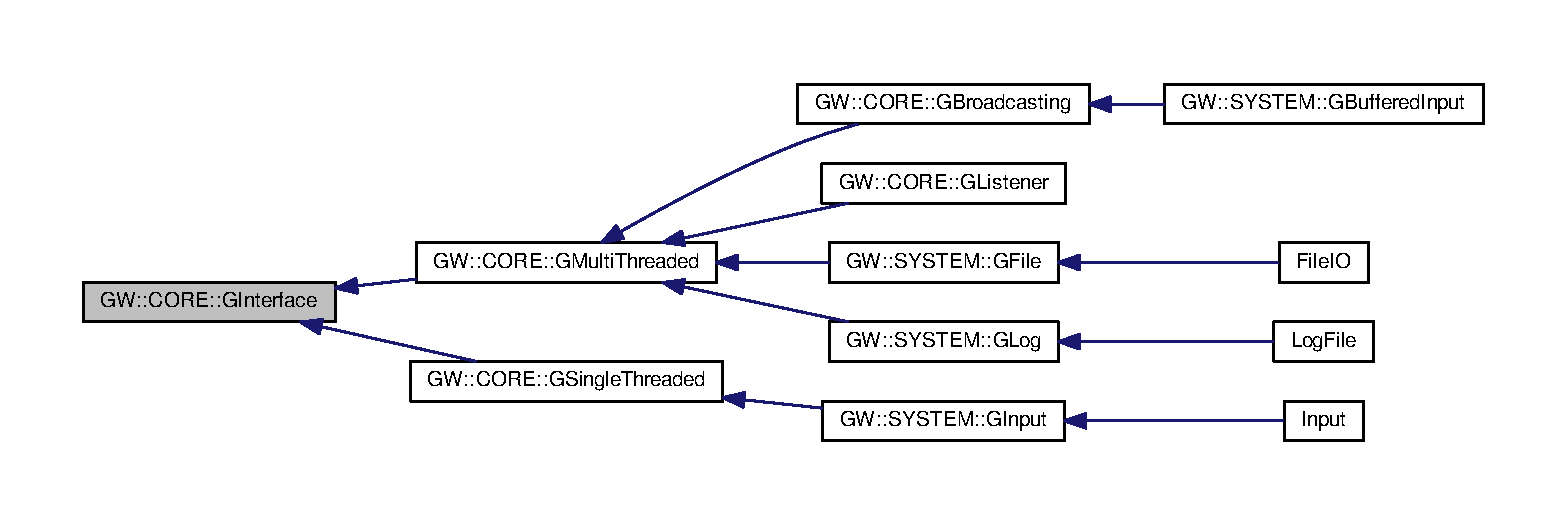
\includegraphics[width=350pt]{classGW_1_1CORE_1_1GInterface__inherit__graph}
\end{center}
\end{figure}
\subsection*{Public Member Functions}
\begin{DoxyCompactItemize}
\item 
virtual \hyperlink{namespaceGW_a67a839e3df7ea8a5c5686613a7a3de21}{G\+Return} \hyperlink{classGW_1_1CORE_1_1GInterface_aacf5834174a7024f8a3c361122ee9e76}{Get\+Count} (unsigned int \&\+\_\+out\+Count)=0
\begin{DoxyCompactList}\small\item\em Return the total number of active references to this object. \end{DoxyCompactList}\item 
virtual \hyperlink{namespaceGW_a67a839e3df7ea8a5c5686613a7a3de21}{G\+Return} \hyperlink{classGW_1_1CORE_1_1GInterface_a2d710f20bb78e544e8309b5b75c21260}{Increment\+Count} ()=0
\begin{DoxyCompactList}\small\item\em Increase the total number of active references to this object. \end{DoxyCompactList}\item 
virtual \hyperlink{namespaceGW_a67a839e3df7ea8a5c5686613a7a3de21}{G\+Return} \hyperlink{classGW_1_1CORE_1_1GInterface_a19a368c77ad0aa7f49b5a4f772f173ba}{Decrement\+Count} ()=0
\begin{DoxyCompactList}\small\item\em Decrease the total number of active references to this object. \end{DoxyCompactList}\item 
virtual \hyperlink{namespaceGW_a67a839e3df7ea8a5c5686613a7a3de21}{G\+Return} \hyperlink{classGW_1_1CORE_1_1GInterface_ad6c8324970172784964f484686d4fdad}{Request\+Interface} (const \hyperlink{structGW_1_1GUUIID}{G\+U\+U\+I\+ID} \&\+\_\+interface\+ID, void $\ast$$\ast$\+\_\+output\+Interface)=0
\begin{DoxyCompactList}\small\item\em Requests an interface that may or may not be supported by this object. \end{DoxyCompactList}\end{DoxyCompactItemize}


\subsection{Detailed Description}
Base interface all Gateware interfaces must support at a minimum. 

Core features include\+: Interface Upgrades, Reference Counting, Event Broadcasting. 

\subsection{Member Function Documentation}
\index{G\+W\+::\+C\+O\+R\+E\+::\+G\+Interface@{G\+W\+::\+C\+O\+R\+E\+::\+G\+Interface}!Decrement\+Count@{Decrement\+Count}}
\index{Decrement\+Count@{Decrement\+Count}!G\+W\+::\+C\+O\+R\+E\+::\+G\+Interface@{G\+W\+::\+C\+O\+R\+E\+::\+G\+Interface}}
\subsubsection[{\texorpdfstring{Decrement\+Count()=0}{DecrementCount()=0}}]{\setlength{\rightskip}{0pt plus 5cm}virtual {\bf G\+Return} G\+W\+::\+C\+O\+R\+E\+::\+G\+Interface\+::\+Decrement\+Count (
\begin{DoxyParamCaption}
{}
\end{DoxyParamCaption}
)\hspace{0.3cm}{\ttfamily [pure virtual]}}\hypertarget{classGW_1_1CORE_1_1GInterface_a19a368c77ad0aa7f49b5a4f772f173ba}{}\label{classGW_1_1CORE_1_1GInterface_a19a368c77ad0aa7f49b5a4f772f173ba}


Decrease the total number of active references to this object. 

Once the internal count reaches zero this object will be deallocated and your pointer will become invalid.


\begin{DoxyRetVals}{Return values}
{\em S\+U\+C\+C\+E\+SS} & Successfully decremented the internal reference count. \\
\hline
{\em F\+A\+I\+L\+U\+RE} & Decrementing of internal reference count would underflow the value. \\
\hline
\end{DoxyRetVals}


Implemented in \hyperlink{classFileIO_ab7e4806ca819c3fcdeeb40a2af5f0298}{File\+IO}, \hyperlink{classLogFile_a555ef35fcdce23ebad05f7dcabaf0757}{Log\+File}, and \hyperlink{classInput_a5c44b3dc2be21c1bad5f32a43a7b7a55}{Input}.

\index{G\+W\+::\+C\+O\+R\+E\+::\+G\+Interface@{G\+W\+::\+C\+O\+R\+E\+::\+G\+Interface}!Get\+Count@{Get\+Count}}
\index{Get\+Count@{Get\+Count}!G\+W\+::\+C\+O\+R\+E\+::\+G\+Interface@{G\+W\+::\+C\+O\+R\+E\+::\+G\+Interface}}
\subsubsection[{\texorpdfstring{Get\+Count(unsigned int \&\+\_\+out\+Count)=0}{GetCount(unsigned int &_outCount)=0}}]{\setlength{\rightskip}{0pt plus 5cm}virtual {\bf G\+Return} G\+W\+::\+C\+O\+R\+E\+::\+G\+Interface\+::\+Get\+Count (
\begin{DoxyParamCaption}
\item[{unsigned int \&}]{\+\_\+out\+Count}
\end{DoxyParamCaption}
)\hspace{0.3cm}{\ttfamily [pure virtual]}}\hypertarget{classGW_1_1CORE_1_1GInterface_aacf5834174a7024f8a3c361122ee9e76}{}\label{classGW_1_1CORE_1_1GInterface_aacf5834174a7024f8a3c361122ee9e76}


Return the total number of active references to this object. 


\begin{DoxyParams}[1]{Parameters}
\mbox{\tt out}  & {\em \+\_\+out\+Count} & The total number of active references of this object.\\
\hline
\end{DoxyParams}

\begin{DoxyRetVals}{Return values}
{\em S\+U\+C\+C\+E\+SS} & Successfully ran. \\
\hline
{\em F\+A\+I\+L\+U\+RE} & Either class does not exist or the internal reference count is corrupt. \\
\hline
\end{DoxyRetVals}


Implemented in \hyperlink{classFileIO_a20566e320ec4cc0d5615bc3bc1fa3013}{File\+IO}, \hyperlink{classLogFile_ab2abbdb01e2b904f112e5e7b20c59a81}{Log\+File}, and \hyperlink{classInput_a2fd6659ae76357836c4c9b3e7070ffb0}{Input}.

\index{G\+W\+::\+C\+O\+R\+E\+::\+G\+Interface@{G\+W\+::\+C\+O\+R\+E\+::\+G\+Interface}!Increment\+Count@{Increment\+Count}}
\index{Increment\+Count@{Increment\+Count}!G\+W\+::\+C\+O\+R\+E\+::\+G\+Interface@{G\+W\+::\+C\+O\+R\+E\+::\+G\+Interface}}
\subsubsection[{\texorpdfstring{Increment\+Count()=0}{IncrementCount()=0}}]{\setlength{\rightskip}{0pt plus 5cm}virtual {\bf G\+Return} G\+W\+::\+C\+O\+R\+E\+::\+G\+Interface\+::\+Increment\+Count (
\begin{DoxyParamCaption}
{}
\end{DoxyParamCaption}
)\hspace{0.3cm}{\ttfamily [pure virtual]}}\hypertarget{classGW_1_1CORE_1_1GInterface_a2d710f20bb78e544e8309b5b75c21260}{}\label{classGW_1_1CORE_1_1GInterface_a2d710f20bb78e544e8309b5b75c21260}


Increase the total number of active references to this object. 

End users should only call this operation if they are familiar with reference counting behavior.


\begin{DoxyRetVals}{Return values}
{\em S\+U\+C\+C\+E\+SS} & Successfully incremented the internal reference count. \\
\hline
{\em F\+A\+I\+L\+U\+RE} & Incrementation of internal reference count would overflow the value. \\
\hline
\end{DoxyRetVals}


Implemented in \hyperlink{classFileIO_a9f2c9a4d13577e14a2c94b0e9617d80b}{File\+IO}, \hyperlink{classLogFile_aff5871b4f2434b6ca722b89581416da0}{Log\+File}, and \hyperlink{classInput_a3c2103023cbb1fa583f910539bb6cce3}{Input}.

\index{G\+W\+::\+C\+O\+R\+E\+::\+G\+Interface@{G\+W\+::\+C\+O\+R\+E\+::\+G\+Interface}!Request\+Interface@{Request\+Interface}}
\index{Request\+Interface@{Request\+Interface}!G\+W\+::\+C\+O\+R\+E\+::\+G\+Interface@{G\+W\+::\+C\+O\+R\+E\+::\+G\+Interface}}
\subsubsection[{\texorpdfstring{Request\+Interface(const G\+U\+U\+I\+I\+D \&\+\_\+interface\+I\+D, void $\ast$$\ast$\+\_\+output\+Interface)=0}{RequestInterface(const GUUIID &_interfaceID, void **_outputInterface)=0}}]{\setlength{\rightskip}{0pt plus 5cm}virtual {\bf G\+Return} G\+W\+::\+C\+O\+R\+E\+::\+G\+Interface\+::\+Request\+Interface (
\begin{DoxyParamCaption}
\item[{const {\bf G\+U\+U\+I\+ID} \&}]{\+\_\+interface\+ID, }
\item[{void $\ast$$\ast$}]{\+\_\+output\+Interface}
\end{DoxyParamCaption}
)\hspace{0.3cm}{\ttfamily [pure virtual]}}\hypertarget{classGW_1_1CORE_1_1GInterface_ad6c8324970172784964f484686d4fdad}{}\label{classGW_1_1CORE_1_1GInterface_ad6c8324970172784964f484686d4fdad}


Requests an interface that may or may not be supported by this object. 

Can be used by the end-\/user to query for a new interface using the unique ID of the interface they want and implement an interface update.


\begin{DoxyParams}[1]{Parameters}
\mbox{\tt in}  & {\em \+\_\+interface\+ID} & The \hyperlink{structGW_1_1GUUIID}{G\+U\+U\+I\+ID} of the interface you are requesting. \\
\hline
\mbox{\tt out}  & {\em \+\_\+output\+Interface} & Where the interface will be stored if function is successful.\\
\hline
\end{DoxyParams}

\begin{DoxyRetVals}{Return values}
{\em S\+U\+C\+C\+E\+SS} & The interface is supported and function succeded. \\
\hline
{\em I\+N\+T\+E\+R\+F\+A\+C\+E\+\_\+\+U\+N\+S\+U\+P\+P\+O\+R\+T\+ED} & The requested interface is not supported. \\
\hline
\end{DoxyRetVals}


Implemented in \hyperlink{classFileIO_a3fb39527fac479474c6ef5045dbc1551}{File\+IO}, \hyperlink{classLogFile_a8b8e63b9c62846b1b9e0cf8b79429ba5}{Log\+File}, and \hyperlink{classInput_a29f3c56e9fec9f9073c1e18f120a69cd}{Input}.



The documentation for this class was generated from the following file\+:\begin{DoxyCompactItemize}
\item 
Interface/\+G\+\_\+\+Core/G\+Interface.\+h\end{DoxyCompactItemize}

\hypertarget{classGW_1_1CORE_1_1GListener}{}\section{GW\+::C\+O\+RE\+::G\+Listener Class Reference}
\label{classGW_1_1CORE_1_1GListener}\index{GW::CORE::GListener@{GW::CORE::GListener}}


A \mbox{\hyperlink{classGW_1_1CORE_1_1GListener}{G\+Listener}} Interface may be registered with a G\+Broadcaster interface to receive event notifications.  




{\ttfamily \#include $<$G\+Listener.\+h$>$}



Inheritance diagram for GW\+::C\+O\+RE\+::G\+Listener\+:
% FIG 0


Collaboration diagram for GW\+::C\+O\+RE\+::G\+Listener\+:
% FIG 1
\subsection*{Public Member Functions}
\begin{DoxyCompactItemize}
\item 
virtual \mbox{\hyperlink{namespaceGW_a67a839e3df7ea8a5c5686613a7a3de21}{G\+Return}} \mbox{\hyperlink{classGW_1_1CORE_1_1GListener_a5c1d1fac213b7a1cc15d384aa0c33105}{On\+Event}} (const \mbox{\hyperlink{structGW_1_1GUUIID}{G\+U\+U\+I\+ID}} \&\+\_\+sender\+Interface, unsigned int \+\_\+event\+ID, void $\ast$\+\_\+event\+Data, unsigned int \+\_\+data\+Size)=0
\begin{DoxyCompactList}\small\item\em This operation is called whenever a G\+Broadcaster a listener is registered to generates an event. \end{DoxyCompactList}\end{DoxyCompactItemize}


\subsection{Detailed Description}
A \mbox{\hyperlink{classGW_1_1CORE_1_1GListener}{G\+Listener}} Interface may be registered with a G\+Broadcaster interface to receive event notifications. 

\mbox{\hyperlink{classGW_1_1CORE_1_1GListener}{G\+Listener}} is directly inherited from \mbox{\hyperlink{classGW_1_1CORE_1_1GMultiThreaded}{G\+Multi\+Threaded}}, therefore its implementation must be thread safe. 

\subsection{Member Function Documentation}
\mbox{\Hypertarget{classGW_1_1CORE_1_1GListener_a5c1d1fac213b7a1cc15d384aa0c33105}\label{classGW_1_1CORE_1_1GListener_a5c1d1fac213b7a1cc15d384aa0c33105}} 
\index{GW::CORE::GListener@{GW::CORE::GListener}!OnEvent@{OnEvent}}
\index{OnEvent@{OnEvent}!GW::CORE::GListener@{GW::CORE::GListener}}
\subsubsection{\texorpdfstring{OnEvent()}{OnEvent()}}
{\footnotesize\ttfamily virtual \mbox{\hyperlink{namespaceGW_a67a839e3df7ea8a5c5686613a7a3de21}{G\+Return}} G\+W\+::\+C\+O\+R\+E\+::\+G\+Listener\+::\+On\+Event (\begin{DoxyParamCaption}\item[{const \mbox{\hyperlink{structGW_1_1GUUIID}{G\+U\+U\+I\+ID}} \&}]{\+\_\+sender\+Interface,  }\item[{unsigned int}]{\+\_\+event\+ID,  }\item[{void $\ast$}]{\+\_\+event\+Data,  }\item[{unsigned int}]{\+\_\+data\+Size }\end{DoxyParamCaption})\hspace{0.3cm}{\ttfamily [pure virtual]}}



This operation is called whenever a G\+Broadcaster a listener is registered to generates an event. 


\begin{DoxyParams}[1]{Parameters}
\mbox{\texttt{ in}}  & {\em \+\_\+sender\+Interface} & The interface of the sender object. \\
\hline
\mbox{\texttt{ in}}  & {\em \+\_\+event\+ID} & The ID of the event sent. \\
\hline
\mbox{\texttt{ in}}  & {\em \+\_\+event\+Data} & The data of the event. \\
\hline
\mbox{\texttt{ in}}  & {\em \+\_\+data\+Size} & The size of \+\_\+event\+Data in bytes. \\
\hline
\end{DoxyParams}


The documentation for this class was generated from the following file\+:\begin{DoxyCompactItemize}
\item 
Interface/\+G\+\_\+\+Core/G\+Listener.\+h\end{DoxyCompactItemize}

\hypertarget{classGW_1_1SYSTEM_1_1GLog}{}\section{GW\+:\+:S\+Y\+S\+T\+EM\+:\+:G\+Log Class Reference}
\label{classGW_1_1SYSTEM_1_1GLog}\index{G\+W\+::\+S\+Y\+S\+T\+E\+M\+::\+G\+Log@{G\+W\+::\+S\+Y\+S\+T\+E\+M\+::\+G\+Log}}


Cross platform threadsafe logger.  




{\ttfamily \#include $<$G\+Log.\+h$>$}



Inheritance diagram for GW\+:\+:S\+Y\+S\+T\+EM\+:\+:G\+Log\+:
\nopagebreak
\begin{figure}[H]
\begin{center}
\leavevmode
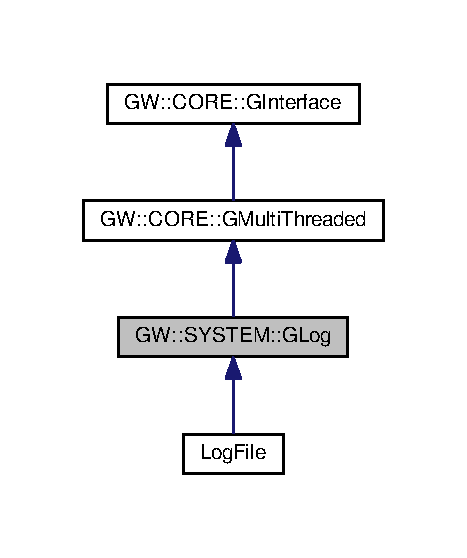
\includegraphics[width=224pt]{classGW_1_1SYSTEM_1_1GLog__inherit__graph}
\end{center}
\end{figure}


Collaboration diagram for GW\+:\+:S\+Y\+S\+T\+EM\+:\+:G\+Log\+:
\nopagebreak
\begin{figure}[H]
\begin{center}
\leavevmode
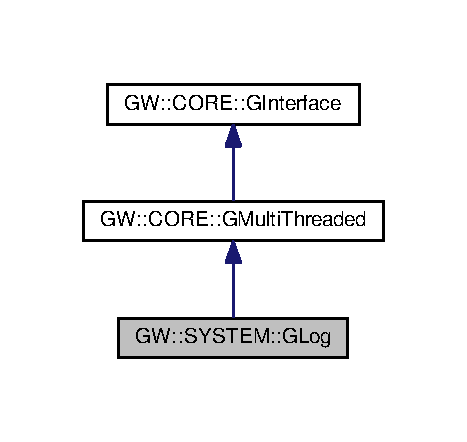
\includegraphics[width=224pt]{classGW_1_1SYSTEM_1_1GLog__coll__graph}
\end{center}
\end{figure}
\subsection*{Public Member Functions}
\begin{DoxyCompactItemize}
\item 
virtual \hyperlink{namespaceGW_a67a839e3df7ea8a5c5686613a7a3de21}{G\+Return} \hyperlink{classGW_1_1SYSTEM_1_1GLog_a9e21e702d012065fe799b4c49f7ac670}{Log} (const char $\ast$const \+\_\+log)=0
\begin{DoxyCompactList}\small\item\em Logs a null terminated string. \end{DoxyCompactList}\item 
virtual \hyperlink{namespaceGW_a67a839e3df7ea8a5c5686613a7a3de21}{G\+Return} \hyperlink{classGW_1_1SYSTEM_1_1GLog_a5d10397fa6aeeebaf8430df6029ec3c5}{Log\+Catergorized} (const char $\ast$const \+\_\+category, const char $\ast$const \+\_\+log)=0
\begin{DoxyCompactList}\small\item\em Logs a null terminated string with a category. \end{DoxyCompactList}\item 
virtual void \hyperlink{classGW_1_1SYSTEM_1_1GLog_a4323c96541a34fb0344828a1c20ec254}{Enable\+Verbose\+Logging} (bool \+\_\+value)=0
\begin{DoxyCompactList}\small\item\em Turns verbose logging on or off. \end{DoxyCompactList}\item 
virtual void \hyperlink{classGW_1_1SYSTEM_1_1GLog_abceb9fdf502b11f2fe72de5edd8f187d}{Enable\+Console\+Logging} (bool \+\_\+value)=0
\begin{DoxyCompactList}\small\item\em Turns console logging on or off. \end{DoxyCompactList}\item 
virtual \hyperlink{namespaceGW_a67a839e3df7ea8a5c5686613a7a3de21}{G\+Return} \hyperlink{classGW_1_1SYSTEM_1_1GLog_a07147c15ecb17caa1c83974b3c54f7d4}{Flush} ()=0
\begin{DoxyCompactList}\small\item\em Forces a log dump to file. \end{DoxyCompactList}\end{DoxyCompactItemize}


\subsection{Detailed Description}
Cross platform threadsafe logger. 

\hyperlink{classGW_1_1SYSTEM_1_1GLog}{G\+Log} inherits directly from G\+Multi\+Threaded, therefore its implementation must be thread safe. 

\subsection{Member Function Documentation}
\index{G\+W\+::\+S\+Y\+S\+T\+E\+M\+::\+G\+Log@{G\+W\+::\+S\+Y\+S\+T\+E\+M\+::\+G\+Log}!Enable\+Console\+Logging@{Enable\+Console\+Logging}}
\index{Enable\+Console\+Logging@{Enable\+Console\+Logging}!G\+W\+::\+S\+Y\+S\+T\+E\+M\+::\+G\+Log@{G\+W\+::\+S\+Y\+S\+T\+E\+M\+::\+G\+Log}}
\subsubsection[{\texorpdfstring{Enable\+Console\+Logging(bool \+\_\+value)=0}{EnableConsoleLogging(bool _value)=0}}]{\setlength{\rightskip}{0pt plus 5cm}virtual void G\+W\+::\+S\+Y\+S\+T\+E\+M\+::\+G\+Log\+::\+Enable\+Console\+Logging (
\begin{DoxyParamCaption}
\item[{bool}]{\+\_\+value}
\end{DoxyParamCaption}
)\hspace{0.3cm}{\ttfamily [pure virtual]}}\hypertarget{classGW_1_1SYSTEM_1_1GLog_abceb9fdf502b11f2fe72de5edd8f187d}{}\label{classGW_1_1SYSTEM_1_1GLog_abceb9fdf502b11f2fe72de5edd8f187d}


Turns console logging on or off. 

Use this function to ensure or prevent the additional console logging.


\begin{DoxyParams}[1]{Parameters}
\mbox{\tt in}  & {\em \+\_\+value} & true to turn on or false to turn off. \\
\hline
\end{DoxyParams}


Implemented in \hyperlink{classLogFile_a903b31947e1c100309dcc5b20548262c}{Log\+File}.

\index{G\+W\+::\+S\+Y\+S\+T\+E\+M\+::\+G\+Log@{G\+W\+::\+S\+Y\+S\+T\+E\+M\+::\+G\+Log}!Enable\+Verbose\+Logging@{Enable\+Verbose\+Logging}}
\index{Enable\+Verbose\+Logging@{Enable\+Verbose\+Logging}!G\+W\+::\+S\+Y\+S\+T\+E\+M\+::\+G\+Log@{G\+W\+::\+S\+Y\+S\+T\+E\+M\+::\+G\+Log}}
\subsubsection[{\texorpdfstring{Enable\+Verbose\+Logging(bool \+\_\+value)=0}{EnableVerboseLogging(bool _value)=0}}]{\setlength{\rightskip}{0pt plus 5cm}virtual void G\+W\+::\+S\+Y\+S\+T\+E\+M\+::\+G\+Log\+::\+Enable\+Verbose\+Logging (
\begin{DoxyParamCaption}
\item[{bool}]{\+\_\+value}
\end{DoxyParamCaption}
)\hspace{0.3cm}{\ttfamily [pure virtual]}}\hypertarget{classGW_1_1SYSTEM_1_1GLog_a4323c96541a34fb0344828a1c20ec254}{}\label{classGW_1_1SYSTEM_1_1GLog_a4323c96541a34fb0344828a1c20ec254}


Turns verbose logging on or off. 

Use this function to ensure or prevent the addition of date, time, and thread\+ID to your log messages.


\begin{DoxyParams}[1]{Parameters}
\mbox{\tt in}  & {\em \+\_\+value} & true to turn on or false to turn off. \\
\hline
\end{DoxyParams}


Implemented in \hyperlink{classLogFile_a250bcfaccded12f7da9a06b6f6336fa5}{Log\+File}.

\index{G\+W\+::\+S\+Y\+S\+T\+E\+M\+::\+G\+Log@{G\+W\+::\+S\+Y\+S\+T\+E\+M\+::\+G\+Log}!Flush@{Flush}}
\index{Flush@{Flush}!G\+W\+::\+S\+Y\+S\+T\+E\+M\+::\+G\+Log@{G\+W\+::\+S\+Y\+S\+T\+E\+M\+::\+G\+Log}}
\subsubsection[{\texorpdfstring{Flush()=0}{Flush()=0}}]{\setlength{\rightskip}{0pt plus 5cm}virtual {\bf G\+Return} G\+W\+::\+S\+Y\+S\+T\+E\+M\+::\+G\+Log\+::\+Flush (
\begin{DoxyParamCaption}
{}
\end{DoxyParamCaption}
)\hspace{0.3cm}{\ttfamily [pure virtual]}}\hypertarget{classGW_1_1SYSTEM_1_1GLog_a07147c15ecb17caa1c83974b3c54f7d4}{}\label{classGW_1_1SYSTEM_1_1GLog_a07147c15ecb17caa1c83974b3c54f7d4}


Forces a log dump to file. 

This will force a log dump to the file and clear the log queue.


\begin{DoxyRetVals}{Return values}
{\em S\+U\+C\+C\+E\+SS} & Successfully dumped the logs. \\
\hline
{\em F\+A\+I\+L\+U\+RE} & Most likely a file corruption or a file is not open. \\
\hline
\end{DoxyRetVals}


Implemented in \hyperlink{classLogFile_a47ffb41f72625b1c7865ac2cd58dea18}{Log\+File}.

\index{G\+W\+::\+S\+Y\+S\+T\+E\+M\+::\+G\+Log@{G\+W\+::\+S\+Y\+S\+T\+E\+M\+::\+G\+Log}!Log@{Log}}
\index{Log@{Log}!G\+W\+::\+S\+Y\+S\+T\+E\+M\+::\+G\+Log@{G\+W\+::\+S\+Y\+S\+T\+E\+M\+::\+G\+Log}}
\subsubsection[{\texorpdfstring{Log(const char $\ast$const \+\_\+log)=0}{Log(const char *const _log)=0}}]{\setlength{\rightskip}{0pt plus 5cm}virtual {\bf G\+Return} G\+W\+::\+S\+Y\+S\+T\+E\+M\+::\+G\+Log\+::\+Log (
\begin{DoxyParamCaption}
\item[{const char $\ast$const}]{\+\_\+log}
\end{DoxyParamCaption}
)\hspace{0.3cm}{\ttfamily [pure virtual]}}\hypertarget{classGW_1_1SYSTEM_1_1GLog_a9e21e702d012065fe799b4c49f7ac670}{}\label{classGW_1_1SYSTEM_1_1GLog_a9e21e702d012065fe799b4c49f7ac670}


Logs a null terminated string. 

Date, Time, and thread ID will be appended to the front of the message unless specified otherwise (See Enable\+Verbose\+Logging). A new line character will be appended to the end of the string so your log messages do not require a new line. The string is logged to the internal \hyperlink{classGW_1_1SYSTEM_1_1GFile}{G\+File} object.


\begin{DoxyParams}[1]{Parameters}
\mbox{\tt in}  & {\em \+\_\+log} & The message to log out.\\
\hline
\end{DoxyParams}

\begin{DoxyRetVals}{Return values}
{\em S\+U\+C\+C\+E\+SS} & Successfully queued the message to the log. \\
\hline
{\em F\+A\+I\+L\+U\+RE} & The queue has reached maximum size (call flush). \\
\hline
{\em I\+N\+V\+A\+L\+I\+D\+\_\+\+A\+R\+G\+U\+M\+E\+NT} & A nullptr was passed in. \\
\hline
\end{DoxyRetVals}


Implemented in \hyperlink{classLogFile_a6848c12fad15f2c835e5215234f75c5a}{Log\+File}.

\index{G\+W\+::\+S\+Y\+S\+T\+E\+M\+::\+G\+Log@{G\+W\+::\+S\+Y\+S\+T\+E\+M\+::\+G\+Log}!Log\+Catergorized@{Log\+Catergorized}}
\index{Log\+Catergorized@{Log\+Catergorized}!G\+W\+::\+S\+Y\+S\+T\+E\+M\+::\+G\+Log@{G\+W\+::\+S\+Y\+S\+T\+E\+M\+::\+G\+Log}}
\subsubsection[{\texorpdfstring{Log\+Catergorized(const char $\ast$const \+\_\+category, const char $\ast$const \+\_\+log)=0}{LogCatergorized(const char *const _category, const char *const _log)=0}}]{\setlength{\rightskip}{0pt plus 5cm}virtual {\bf G\+Return} G\+W\+::\+S\+Y\+S\+T\+E\+M\+::\+G\+Log\+::\+Log\+Catergorized (
\begin{DoxyParamCaption}
\item[{const char $\ast$const}]{\+\_\+category, }
\item[{const char $\ast$const}]{\+\_\+log}
\end{DoxyParamCaption}
)\hspace{0.3cm}{\ttfamily [pure virtual]}}\hypertarget{classGW_1_1SYSTEM_1_1GLog_a5d10397fa6aeeebaf8430df6029ec3c5}{}\label{classGW_1_1SYSTEM_1_1GLog_a5d10397fa6aeeebaf8430df6029ec3c5}


Logs a null terminated string with a category. 

Date, Time, and thread ID will be appended to the front of the message unless specified otherwise (See Enable\+Verbose\+Logging). A new line character will be appended to the end of the string so your log messages do not require a new line. The string is logged to the internal \hyperlink{classGW_1_1SYSTEM_1_1GFile}{G\+File} object.


\begin{DoxyParams}[1]{Parameters}
\mbox{\tt in}  & {\em \+\_\+category} & The category the log belongs in. ie. E\+R\+R\+OR, W\+A\+R\+N\+I\+NG, I\+N\+FO, etc. \\
\hline
\mbox{\tt in}  & {\em \+\_\+log} & The message to log out.\\
\hline
\end{DoxyParams}

\begin{DoxyRetVals}{Return values}
{\em S\+U\+C\+C\+E\+SS} & Successfully queued the message to the log. \\
\hline
{\em F\+A\+I\+L\+U\+RE} & The queue has reached maximum size (call flush). \\
\hline
{\em I\+N\+V\+A\+L\+I\+D\+\_\+\+A\+R\+G\+U\+M\+E\+NT} & Either \+\_\+category or \+\_\+log are nullptr. \\
\hline
\end{DoxyRetVals}


Implemented in \hyperlink{classLogFile_a5e5f24ccd4c6f925dd8bc1ced512b530}{Log\+File}.



The documentation for this class was generated from the following file\+:\begin{DoxyCompactItemize}
\item 
Interface/\+G\+\_\+\+System/G\+Log.\+h\end{DoxyCompactItemize}

\hypertarget{classGW_1_1MATH_1_1GMatrix}{}\section{GW\+:\+:M\+A\+TH\+:\+:G\+Matrix Class Reference}
\label{classGW_1_1MATH_1_1GMatrix}\index{G\+W\+::\+M\+A\+T\+H\+::\+G\+Matrix@{G\+W\+::\+M\+A\+T\+H\+::\+G\+Matrix}}


Matrix functions.  




{\ttfamily \#include $<$G\+Matrix.\+h$>$}



Inheritance diagram for GW\+:\+:M\+A\+TH\+:\+:G\+Matrix\+:
% FIG 0


Collaboration diagram for GW\+:\+:M\+A\+TH\+:\+:G\+Matrix\+:
% FIG 1
\subsection*{Public Member Functions}
\begin{DoxyCompactItemize}
\item 
virtual \hyperlink{namespaceGW_a67a839e3df7ea8a5c5686613a7a3de21}{G\+Return} \hyperlink{classGW_1_1MATH_1_1GMatrix_a40f37f26a141222068d55994b8161cde}{Add\+MatrixF} (\hyperlink{structGW_1_1MATH_1_1GMATRIXF}{G\+M\+A\+T\+R\+I\+XF} \+\_\+matrix1, \hyperlink{structGW_1_1MATH_1_1GMATRIXF}{G\+M\+A\+T\+R\+I\+XF} \+\_\+matrix2, \hyperlink{structGW_1_1MATH_1_1GMATRIXF}{G\+M\+A\+T\+R\+I\+XF} \&\+\_\+out\+Matrix)=0
\begin{DoxyCompactList}\small\item\em Add two specified matirxs. \end{DoxyCompactList}\item 
virtual \hyperlink{namespaceGW_a67a839e3df7ea8a5c5686613a7a3de21}{G\+Return} \hyperlink{classGW_1_1MATH_1_1GMatrix_a0b744e7f36718b8cccf2423c88c43a30}{Subtract\+MatrixF} (\hyperlink{structGW_1_1MATH_1_1GMATRIXF}{G\+M\+A\+T\+R\+I\+XF} \+\_\+matrix1, \hyperlink{structGW_1_1MATH_1_1GMATRIXF}{G\+M\+A\+T\+R\+I\+XF} \+\_\+matrix2, \hyperlink{structGW_1_1MATH_1_1GMATRIXF}{G\+M\+A\+T\+R\+I\+XF} \&\+\_\+out\+Matrix)=0
\begin{DoxyCompactList}\small\item\em Subtract two specified matirxs. \end{DoxyCompactList}\item 
virtual \hyperlink{namespaceGW_a67a839e3df7ea8a5c5686613a7a3de21}{G\+Return} \hyperlink{classGW_1_1MATH_1_1GMatrix_a03ca7a7e5ad97849b9867d0210aa4bc0}{Multiply\+MatrixF} (\hyperlink{structGW_1_1MATH_1_1GMATRIXF}{G\+M\+A\+T\+R\+I\+XF} \+\_\+matrix1, \hyperlink{structGW_1_1MATH_1_1GMATRIXF}{G\+M\+A\+T\+R\+I\+XF} \+\_\+matrix2, \hyperlink{structGW_1_1MATH_1_1GMATRIXF}{G\+M\+A\+T\+R\+I\+XF} \&\+\_\+out\+Matrix)=0
\begin{DoxyCompactList}\small\item\em Multiply two specified matirxs. \end{DoxyCompactList}\item 
virtual \hyperlink{namespaceGW_a67a839e3df7ea8a5c5686613a7a3de21}{G\+Return} \hyperlink{classGW_1_1MATH_1_1GMatrix_a8e1b421243bebab184ca0237e163fa2d}{Vector\+X\+MatrixF} (\hyperlink{structGW_1_1MATH_1_1GMATRIXF}{G\+M\+A\+T\+R\+I\+XF} \+\_\+matrix, \hyperlink{structGW_1_1MATH_1_1GVECTORF}{G\+V\+E\+C\+T\+O\+RF} \+\_\+vector, \hyperlink{structGW_1_1MATH_1_1GVECTORF}{G\+V\+E\+C\+T\+O\+RF} \&\+\_\+out\+Vector)=0
\begin{DoxyCompactList}\small\item\em Multiply the specified matrix by the specified vector. \end{DoxyCompactList}\item 
virtual \hyperlink{namespaceGW_a67a839e3df7ea8a5c5686613a7a3de21}{G\+Return} \hyperlink{classGW_1_1MATH_1_1GMatrix_aded7d8a4b4cd54c3fc7f43bab1ed0730}{Convert\+QuaternionF} (\hyperlink{structGW_1_1MATH_1_1GQUATERNIONF}{G\+Q\+U\+A\+T\+E\+R\+N\+I\+O\+NF} \+\_\+quaternion, \hyperlink{structGW_1_1MATH_1_1GMATRIXF}{G\+M\+A\+T\+R\+I\+XF} \&\+\_\+out\+Matrix)=0
\begin{DoxyCompactList}\small\item\em Convert the specified quaternion to a matrix. \end{DoxyCompactList}\item 
virtual \hyperlink{namespaceGW_a67a839e3df7ea8a5c5686613a7a3de21}{G\+Return} \hyperlink{classGW_1_1MATH_1_1GMatrix_ab2560c150812cd88dd631e533ea5f9dc}{Multiply\+NumF} (\hyperlink{structGW_1_1MATH_1_1GMATRIXF}{G\+M\+A\+T\+R\+I\+XF} \+\_\+matrix, float \+\_\+scalar, \hyperlink{structGW_1_1MATH_1_1GMATRIXF}{G\+M\+A\+T\+R\+I\+XF} \&\+\_\+out\+Matrix)=0
\begin{DoxyCompactList}\small\item\em Scale the matrix. \end{DoxyCompactList}\item 
virtual \hyperlink{namespaceGW_a67a839e3df7ea8a5c5686613a7a3de21}{G\+Return} \hyperlink{classGW_1_1MATH_1_1GMatrix_a8ae14af67e2b099569a4439b7497b37d}{DeterminantF} (\hyperlink{structGW_1_1MATH_1_1GMATRIXF}{G\+M\+A\+T\+R\+I\+XF} \+\_\+matrix, float \&\+\_\+out\+Value)=0
\begin{DoxyCompactList}\small\item\em Calculate the determinant of the specified matirx. \end{DoxyCompactList}\item 
virtual \hyperlink{namespaceGW_a67a839e3df7ea8a5c5686613a7a3de21}{G\+Return} \hyperlink{classGW_1_1MATH_1_1GMatrix_ae1865f48ec9187b508cbcfe083496581}{TransposeF} (\hyperlink{structGW_1_1MATH_1_1GMATRIXF}{G\+M\+A\+T\+R\+I\+XF} \+\_\+matrix, \hyperlink{structGW_1_1MATH_1_1GMATRIXF}{G\+M\+A\+T\+R\+I\+XF} \&\+\_\+out\+Matrix)=0
\begin{DoxyCompactList}\small\item\em Transpose the specified matirx. \end{DoxyCompactList}\item 
virtual \hyperlink{namespaceGW_a67a839e3df7ea8a5c5686613a7a3de21}{G\+Return} \hyperlink{classGW_1_1MATH_1_1GMatrix_a47cbc24d8a15f8cf605f6585c8b44e2e}{InverseF} (\hyperlink{structGW_1_1MATH_1_1GMATRIXF}{G\+M\+A\+T\+R\+I\+XF} \+\_\+matrix, \hyperlink{structGW_1_1MATH_1_1GMATRIXF}{G\+M\+A\+T\+R\+I\+XF} \&\+\_\+out\+Matrix)=0
\begin{DoxyCompactList}\small\item\em Inverse the specified matirx. \end{DoxyCompactList}\item 
virtual \hyperlink{namespaceGW_a67a839e3df7ea8a5c5686613a7a3de21}{G\+Return} \hyperlink{classGW_1_1MATH_1_1GMatrix_aee68de35de388c5893b6fcdd450dd1d3}{IdentityF} (\hyperlink{structGW_1_1MATH_1_1GMATRIXF}{G\+M\+A\+T\+R\+I\+XF} \&\+\_\+out\+Matrix)=0
\begin{DoxyCompactList}\small\item\em Identity the specified matrix. \end{DoxyCompactList}\item 
virtual \hyperlink{namespaceGW_a67a839e3df7ea8a5c5686613a7a3de21}{G\+Return} \hyperlink{classGW_1_1MATH_1_1GMatrix_a1c9745c2b04e1ab4d4446d65c5f0fb89}{Get\+RotationF} (\hyperlink{structGW_1_1MATH_1_1GMATRIXF}{G\+M\+A\+T\+R\+I\+XF} \+\_\+matrix, \hyperlink{structGW_1_1MATH_1_1GQUATERNIONF}{G\+Q\+U\+A\+T\+E\+R\+N\+I\+O\+NF} \&\+\_\+out\+Quaternion)=0
\begin{DoxyCompactList}\small\item\em Get the quaternion which represents the roataion of the specified matrix. \end{DoxyCompactList}\item 
virtual \hyperlink{namespaceGW_a67a839e3df7ea8a5c5686613a7a3de21}{G\+Return} \hyperlink{classGW_1_1MATH_1_1GMatrix_a5948489188390e3566f7a0fcba687c97}{Get\+TranslationF} (\hyperlink{structGW_1_1MATH_1_1GMATRIXF}{G\+M\+A\+T\+R\+I\+XF} \+\_\+matrix, \hyperlink{structGW_1_1MATH_1_1GVECTORF}{G\+V\+E\+C\+T\+O\+RF} \&\+\_\+out\+Matrix)=0
\begin{DoxyCompactList}\small\item\em Get the translation matrix from the specified matrix. \end{DoxyCompactList}\item 
virtual \hyperlink{namespaceGW_a67a839e3df7ea8a5c5686613a7a3de21}{G\+Return} \hyperlink{classGW_1_1MATH_1_1GMatrix_aaf1e6774edbb0d9e2b5074298bcae8dd}{Get\+ScaleF} (\hyperlink{structGW_1_1MATH_1_1GMATRIXF}{G\+M\+A\+T\+R\+I\+XF} \+\_\+matrix, \hyperlink{structGW_1_1MATH_1_1GVECTORF}{G\+V\+E\+C\+T\+O\+RF} \&\+\_\+out\+Matrix)=0
\begin{DoxyCompactList}\small\item\em Get the scaling matrix from the specified matrix. \end{DoxyCompactList}\item 
virtual \hyperlink{namespaceGW_a67a839e3df7ea8a5c5686613a7a3de21}{G\+Return} \hyperlink{classGW_1_1MATH_1_1GMatrix_acd8ef29804a2d807876b2f0a22a1f9b4}{Rotation\+XF} (\hyperlink{structGW_1_1MATH_1_1GMATRIXF}{G\+M\+A\+T\+R\+I\+XF} \+\_\+matrix, float \+\_\+radian, \hyperlink{structGW_1_1MATH_1_1GMATRIXF}{G\+M\+A\+T\+R\+I\+XF} \&\+\_\+out\+Matrix)=0
\begin{DoxyCompactList}\small\item\em Roatate the specified matrix around the x-\/axis by multiplying a left-\/handed rotation matrix. \end{DoxyCompactList}\item 
virtual \hyperlink{namespaceGW_a67a839e3df7ea8a5c5686613a7a3de21}{G\+Return} \hyperlink{classGW_1_1MATH_1_1GMatrix_afe5fa5399691dc690272dad5d3697ff9}{Rotation\+YF} (\hyperlink{structGW_1_1MATH_1_1GMATRIXF}{G\+M\+A\+T\+R\+I\+XF} \+\_\+matrix, float \+\_\+radian, \hyperlink{structGW_1_1MATH_1_1GMATRIXF}{G\+M\+A\+T\+R\+I\+XF} \&\+\_\+out\+Matrix)=0
\begin{DoxyCompactList}\small\item\em Roatate the specified matrix around the y-\/axis by multiplying a left-\/handed rotation matrix. \end{DoxyCompactList}\item 
virtual \hyperlink{namespaceGW_a67a839e3df7ea8a5c5686613a7a3de21}{G\+Return} \hyperlink{classGW_1_1MATH_1_1GMatrix_abce415225da8aa2592e1ef495fd9996b}{Rotation\+ZF} (\hyperlink{structGW_1_1MATH_1_1GMATRIXF}{G\+M\+A\+T\+R\+I\+XF} \+\_\+matrix, float \+\_\+radian, \hyperlink{structGW_1_1MATH_1_1GMATRIXF}{G\+M\+A\+T\+R\+I\+XF} \&\+\_\+out\+Matrix)=0
\begin{DoxyCompactList}\small\item\em Roatate the specified matrix around the z-\/axis by multiplying a left-\/handed rotation matrix. \end{DoxyCompactList}\item 
virtual \hyperlink{namespaceGW_a67a839e3df7ea8a5c5686613a7a3de21}{G\+Return} \hyperlink{classGW_1_1MATH_1_1GMatrix_a821ff1b8cda633278f4d0088d2063d4d}{Rotation\+Yaw\+Pitch\+RollF} (float \+\_\+yaw, float \+\_\+pitch, float \+\_\+roll, \hyperlink{structGW_1_1MATH_1_1GMATRIXF}{G\+M\+A\+T\+R\+I\+XF} \&\+\_\+out\+Matrix)=0
\begin{DoxyCompactList}\small\item\em Builds a matrix based on specified yaw, pitch, and roll angles in radian. \end{DoxyCompactList}\item 
virtual \hyperlink{namespaceGW_a67a839e3df7ea8a5c5686613a7a3de21}{G\+Return} \hyperlink{classGW_1_1MATH_1_1GMatrix_a2dded0d4aa97a7b6c1b885292a441574}{Rotation\+By\+VectorF} (\hyperlink{structGW_1_1MATH_1_1GVECTORF}{G\+V\+E\+C\+T\+O\+RF} \+\_\+vector, float \+\_\+radian, \hyperlink{structGW_1_1MATH_1_1GMATRIXF}{G\+M\+A\+T\+R\+I\+XF} \&\+\_\+out\+Matrix)=0
\begin{DoxyCompactList}\small\item\em Builds a rotation matrix based on specified vector and an angle in radian. \end{DoxyCompactList}\item 
virtual \hyperlink{namespaceGW_a67a839e3df7ea8a5c5686613a7a3de21}{G\+Return} \hyperlink{classGW_1_1MATH_1_1GMatrix_aee43c6ff9c28dbac026b529bef61c236}{TranslatelocalF} (\hyperlink{structGW_1_1MATH_1_1GMATRIXF}{G\+M\+A\+T\+R\+I\+XF} \+\_\+matrix, \hyperlink{structGW_1_1MATH_1_1GVECTORF}{G\+V\+E\+C\+T\+O\+RF} \+\_\+vector, \hyperlink{structGW_1_1MATH_1_1GMATRIXF}{G\+M\+A\+T\+R\+I\+XF} \&\+\_\+out\+Matrix)=0
\begin{DoxyCompactList}\small\item\em Translate the matrix by the specified vector. \end{DoxyCompactList}\item 
virtual \hyperlink{namespaceGW_a67a839e3df7ea8a5c5686613a7a3de21}{G\+Return} \hyperlink{classGW_1_1MATH_1_1GMatrix_a4342d54e82d03d18e493368e87e90137}{ScalingF} (\hyperlink{structGW_1_1MATH_1_1GMATRIXF}{G\+M\+A\+T\+R\+I\+XF} \+\_\+matrix, \hyperlink{structGW_1_1MATH_1_1GVECTORF}{G\+V\+E\+C\+T\+O\+RF} \+\_\+vector, \hyperlink{structGW_1_1MATH_1_1GMATRIXF}{G\+M\+A\+T\+R\+I\+XF} \&\+\_\+out\+Matirx)=0
\begin{DoxyCompactList}\small\item\em Scale the matrix by the specified vector. \end{DoxyCompactList}\item 
virtual \hyperlink{namespaceGW_a67a839e3df7ea8a5c5686613a7a3de21}{G\+Return} \hyperlink{classGW_1_1MATH_1_1GMatrix_a677534c072e7cb8d93223fdc05ae1957}{LerpF} (\hyperlink{structGW_1_1MATH_1_1GMATRIXF}{G\+M\+A\+T\+R\+I\+XF} \+\_\+matrix1, \hyperlink{structGW_1_1MATH_1_1GMATRIXF}{G\+M\+A\+T\+R\+I\+XF} \+\_\+matrix2, float \+\_\+ratio, \hyperlink{structGW_1_1MATH_1_1GMATRIXF}{G\+M\+A\+T\+R\+I\+XF} \&\+\_\+out\+Matrix)=0
\begin{DoxyCompactList}\small\item\em Linearly interpolates between two matrices. \end{DoxyCompactList}\item 
virtual \hyperlink{namespaceGW_a67a839e3df7ea8a5c5686613a7a3de21}{G\+Return} \hyperlink{classGW_1_1MATH_1_1GMatrix_a1e46cce75764e9b92a31a84ceb9ffc3b}{Projection\+L\+HF} (float \+\_\+fovY, float \+\_\+aspect, float \+\_\+zn, float \+\_\+zf, \hyperlink{structGW_1_1MATH_1_1GMATRIXF}{G\+M\+A\+T\+R\+I\+XF} \&\+\_\+out\+Matrix)=0
\begin{DoxyCompactList}\small\item\em Builds a left-\/handed perspective matrix. \end{DoxyCompactList}\item 
virtual \hyperlink{namespaceGW_a67a839e3df7ea8a5c5686613a7a3de21}{G\+Return} \hyperlink{classGW_1_1MATH_1_1GMatrix_a33fa9f8f7f8b700f170d1e2654bbfc3b}{Look\+At\+L\+HF} (\hyperlink{structGW_1_1MATH_1_1GVECTORF}{G\+V\+E\+C\+T\+O\+RF} \+\_\+eye, \hyperlink{structGW_1_1MATH_1_1GVECTORF}{G\+V\+E\+C\+T\+O\+RF} \+\_\+at, \hyperlink{structGW_1_1MATH_1_1GVECTORF}{G\+V\+E\+C\+T\+O\+RF} \+\_\+up, \hyperlink{structGW_1_1MATH_1_1GMATRIXF}{G\+M\+A\+T\+R\+I\+XF} \&\+\_\+out\+Matrix)=0
\begin{DoxyCompactList}\small\item\em Builds a left-\/handed view matrix. \end{DoxyCompactList}\item 
virtual \hyperlink{namespaceGW_a67a839e3df7ea8a5c5686613a7a3de21}{G\+Return} \hyperlink{classGW_1_1MATH_1_1GMatrix_a9ae855c7cfbfa08c84bd76a556302bc5}{Add\+MatrixD} (\hyperlink{structGW_1_1MATH_1_1GMATRIXD}{G\+M\+A\+T\+R\+I\+XD} \+\_\+matrix1, \hyperlink{structGW_1_1MATH_1_1GMATRIXD}{G\+M\+A\+T\+R\+I\+XD} \+\_\+matrix2, \hyperlink{structGW_1_1MATH_1_1GMATRIXD}{G\+M\+A\+T\+R\+I\+XD} \&\+\_\+out\+Matrix)=0
\begin{DoxyCompactList}\small\item\em Add two specified matirxs. \end{DoxyCompactList}\item 
virtual \hyperlink{namespaceGW_a67a839e3df7ea8a5c5686613a7a3de21}{G\+Return} \hyperlink{classGW_1_1MATH_1_1GMatrix_a64478828c2d51b739dd116d948cb4ac3}{Subtract\+MatrixD} (\hyperlink{structGW_1_1MATH_1_1GMATRIXD}{G\+M\+A\+T\+R\+I\+XD} \+\_\+matrix1, \hyperlink{structGW_1_1MATH_1_1GMATRIXD}{G\+M\+A\+T\+R\+I\+XD} \+\_\+matrix2, \hyperlink{structGW_1_1MATH_1_1GMATRIXD}{G\+M\+A\+T\+R\+I\+XD} \&\+\_\+out\+Matrix)=0
\begin{DoxyCompactList}\small\item\em Subtract two specified matirxs. \end{DoxyCompactList}\item 
virtual \hyperlink{namespaceGW_a67a839e3df7ea8a5c5686613a7a3de21}{G\+Return} \hyperlink{classGW_1_1MATH_1_1GMatrix_a613bcf953961899b45e6d97fc5afc2e1}{Multiply\+MatrixD} (\hyperlink{structGW_1_1MATH_1_1GMATRIXD}{G\+M\+A\+T\+R\+I\+XD} \+\_\+matrix1, \hyperlink{structGW_1_1MATH_1_1GMATRIXD}{G\+M\+A\+T\+R\+I\+XD} \+\_\+matrix2, \hyperlink{structGW_1_1MATH_1_1GMATRIXD}{G\+M\+A\+T\+R\+I\+XD} \&\+\_\+out\+Matrix)=0
\begin{DoxyCompactList}\small\item\em Multiply two specified matirxs. \end{DoxyCompactList}\item 
virtual \hyperlink{namespaceGW_a67a839e3df7ea8a5c5686613a7a3de21}{G\+Return} \hyperlink{classGW_1_1MATH_1_1GMatrix_a97cb7b6353e8f89405e44b09390a67cb}{Vector\+X\+MatrixD} (\hyperlink{structGW_1_1MATH_1_1GMATRIXD}{G\+M\+A\+T\+R\+I\+XD} \+\_\+matrix, \hyperlink{structGW_1_1MATH_1_1GVECTORD}{G\+V\+E\+C\+T\+O\+RD} \+\_\+vector, \hyperlink{structGW_1_1MATH_1_1GVECTORD}{G\+V\+E\+C\+T\+O\+RD} \&\+\_\+out\+Vector)=0
\begin{DoxyCompactList}\small\item\em Multiply the specified matrix by the specified vector. \end{DoxyCompactList}\item 
virtual \hyperlink{namespaceGW_a67a839e3df7ea8a5c5686613a7a3de21}{G\+Return} \hyperlink{classGW_1_1MATH_1_1GMatrix_a602c82afc9b9f55c10d6a61da54dcb6c}{Convert\+QuaternionD} (\hyperlink{structGW_1_1MATH_1_1GQUATERNIOND}{G\+Q\+U\+A\+T\+E\+R\+N\+I\+O\+ND} \+\_\+quaternion, \hyperlink{structGW_1_1MATH_1_1GMATRIXD}{G\+M\+A\+T\+R\+I\+XD} \&\+\_\+out\+Matrix)=0
\begin{DoxyCompactList}\small\item\em Convert the specified quaternion to a matrix. \end{DoxyCompactList}\item 
virtual \hyperlink{namespaceGW_a67a839e3df7ea8a5c5686613a7a3de21}{G\+Return} \hyperlink{classGW_1_1MATH_1_1GMatrix_a34e78f82e720eba937824cdc06490b9c}{Multiply\+NumD} (\hyperlink{structGW_1_1MATH_1_1GMATRIXD}{G\+M\+A\+T\+R\+I\+XD} \+\_\+matrix, double \+\_\+scalar, \hyperlink{structGW_1_1MATH_1_1GMATRIXD}{G\+M\+A\+T\+R\+I\+XD} \&\+\_\+out\+Matrix)=0
\begin{DoxyCompactList}\small\item\em Scale the matrix. \end{DoxyCompactList}\item 
virtual \hyperlink{namespaceGW_a67a839e3df7ea8a5c5686613a7a3de21}{G\+Return} \hyperlink{classGW_1_1MATH_1_1GMatrix_ab1b528820ac0476f8f3d9202a3036b8c}{DeterminantD} (\hyperlink{structGW_1_1MATH_1_1GMATRIXD}{G\+M\+A\+T\+R\+I\+XD} \+\_\+matrix, double \&\+\_\+out\+Value)=0
\begin{DoxyCompactList}\small\item\em Calculate the determinant of the specified matirx. \end{DoxyCompactList}\item 
virtual \hyperlink{namespaceGW_a67a839e3df7ea8a5c5686613a7a3de21}{G\+Return} \hyperlink{classGW_1_1MATH_1_1GMatrix_add9f6f4f4689e683143990b434248404}{TransposeD} (\hyperlink{structGW_1_1MATH_1_1GMATRIXD}{G\+M\+A\+T\+R\+I\+XD} \+\_\+matrix, \hyperlink{structGW_1_1MATH_1_1GMATRIXD}{G\+M\+A\+T\+R\+I\+XD} \&\+\_\+out\+Matrix)=0
\begin{DoxyCompactList}\small\item\em Transpose the specified matirx. \end{DoxyCompactList}\item 
virtual \hyperlink{namespaceGW_a67a839e3df7ea8a5c5686613a7a3de21}{G\+Return} \hyperlink{classGW_1_1MATH_1_1GMatrix_ade39ff1c70cb06889196893aad819244}{InverseD} (\hyperlink{structGW_1_1MATH_1_1GMATRIXD}{G\+M\+A\+T\+R\+I\+XD} \+\_\+matrix, \hyperlink{structGW_1_1MATH_1_1GMATRIXD}{G\+M\+A\+T\+R\+I\+XD} \&\+\_\+out\+Matrix)=0
\begin{DoxyCompactList}\small\item\em Inverse the specified matirx. \end{DoxyCompactList}\item 
virtual \hyperlink{namespaceGW_a67a839e3df7ea8a5c5686613a7a3de21}{G\+Return} \hyperlink{classGW_1_1MATH_1_1GMatrix_a3b7136d0cbc99d1a29d159838b5e1d91}{IdentityD} (\hyperlink{structGW_1_1MATH_1_1GMATRIXD}{G\+M\+A\+T\+R\+I\+XD} \&\+\_\+out\+Matrix)=0
\begin{DoxyCompactList}\small\item\em Identity the specified matrix. \end{DoxyCompactList}\item 
virtual \hyperlink{namespaceGW_a67a839e3df7ea8a5c5686613a7a3de21}{G\+Return} \hyperlink{classGW_1_1MATH_1_1GMatrix_aa8a09092d814d7599f2ddedb6a34d1ea}{Get\+RotationD} (\hyperlink{structGW_1_1MATH_1_1GMATRIXD}{G\+M\+A\+T\+R\+I\+XD} \+\_\+matrix, \hyperlink{structGW_1_1MATH_1_1GQUATERNIOND}{G\+Q\+U\+A\+T\+E\+R\+N\+I\+O\+ND} \&\+\_\+out\+Quaternion)=0
\begin{DoxyCompactList}\small\item\em Get the quaternion which represents the roataion of the specified matrix. \end{DoxyCompactList}\item 
virtual \hyperlink{namespaceGW_a67a839e3df7ea8a5c5686613a7a3de21}{G\+Return} \hyperlink{classGW_1_1MATH_1_1GMatrix_a2b2dd5bfce9dc5f567a793ab2a21bb07}{Get\+TranslationD} (\hyperlink{structGW_1_1MATH_1_1GMATRIXD}{G\+M\+A\+T\+R\+I\+XD} \+\_\+matrix, \hyperlink{structGW_1_1MATH_1_1GVECTORD}{G\+V\+E\+C\+T\+O\+RD} \&\+\_\+out\+Matrix)=0
\begin{DoxyCompactList}\small\item\em Get the translation matrix from the specified matrix. \end{DoxyCompactList}\item 
virtual \hyperlink{namespaceGW_a67a839e3df7ea8a5c5686613a7a3de21}{G\+Return} \hyperlink{classGW_1_1MATH_1_1GMatrix_a1d8d370c39617b8ad0fcfb42459fcb09}{Get\+ScaleD} (\hyperlink{structGW_1_1MATH_1_1GMATRIXD}{G\+M\+A\+T\+R\+I\+XD} \+\_\+matrix, \hyperlink{structGW_1_1MATH_1_1GVECTORD}{G\+V\+E\+C\+T\+O\+RD} \&\+\_\+out\+Matrix)=0
\begin{DoxyCompactList}\small\item\em Get the scaling matrix from the specified matrix. \end{DoxyCompactList}\item 
virtual \hyperlink{namespaceGW_a67a839e3df7ea8a5c5686613a7a3de21}{G\+Return} \hyperlink{classGW_1_1MATH_1_1GMatrix_abb2cbb56bb2f3963807e20ba0fe591b3}{Rotation\+XD} (\hyperlink{structGW_1_1MATH_1_1GMATRIXD}{G\+M\+A\+T\+R\+I\+XD} \+\_\+matrix, double \+\_\+radian, \hyperlink{structGW_1_1MATH_1_1GMATRIXD}{G\+M\+A\+T\+R\+I\+XD} \&\+\_\+out\+Matrix)=0
\begin{DoxyCompactList}\small\item\em Roatate the specified matrix around the x-\/axis by multiplying a left-\/handed rotation matrix. \end{DoxyCompactList}\item 
virtual \hyperlink{namespaceGW_a67a839e3df7ea8a5c5686613a7a3de21}{G\+Return} \hyperlink{classGW_1_1MATH_1_1GMatrix_a1f836790e81a0da00ad7e9e5b06969d4}{Rotation\+YD} (\hyperlink{structGW_1_1MATH_1_1GMATRIXD}{G\+M\+A\+T\+R\+I\+XD} \+\_\+matrix, double \+\_\+radian, \hyperlink{structGW_1_1MATH_1_1GMATRIXD}{G\+M\+A\+T\+R\+I\+XD} \&\+\_\+out\+Matrix)=0
\begin{DoxyCompactList}\small\item\em Roatate the specified matrix around the y-\/axis by multiplying a left-\/handed rotation matrix. \end{DoxyCompactList}\item 
virtual \hyperlink{namespaceGW_a67a839e3df7ea8a5c5686613a7a3de21}{G\+Return} \hyperlink{classGW_1_1MATH_1_1GMatrix_ae219f6b6aeddcd2969e5812c8e0a481c}{Rotation\+ZD} (\hyperlink{structGW_1_1MATH_1_1GMATRIXD}{G\+M\+A\+T\+R\+I\+XD} \+\_\+matrix, double \+\_\+radian, \hyperlink{structGW_1_1MATH_1_1GMATRIXD}{G\+M\+A\+T\+R\+I\+XD} \&\+\_\+out\+Matrix)=0
\begin{DoxyCompactList}\small\item\em Roatate the specified matrix around the z-\/axis by multiplying a left-\/handed rotation matrix. \end{DoxyCompactList}\item 
virtual \hyperlink{namespaceGW_a67a839e3df7ea8a5c5686613a7a3de21}{G\+Return} \hyperlink{classGW_1_1MATH_1_1GMatrix_ae63a0eacd6030eeed28dec461986e322}{Rotation\+Yaw\+Pitch\+RollD} (double \+\_\+yaw, double \+\_\+pitch, double \+\_\+roll, \hyperlink{structGW_1_1MATH_1_1GMATRIXD}{G\+M\+A\+T\+R\+I\+XD} \&\+\_\+out\+Matrix)=0
\begin{DoxyCompactList}\small\item\em Builds a matrix based on specified yaw, pitch, and roll angles in radian. \end{DoxyCompactList}\item 
virtual \hyperlink{namespaceGW_a67a839e3df7ea8a5c5686613a7a3de21}{G\+Return} \hyperlink{classGW_1_1MATH_1_1GMatrix_a7262ab71d767293693314c60076652fe}{Rotation\+By\+VectorD} (\hyperlink{structGW_1_1MATH_1_1GVECTORD}{G\+V\+E\+C\+T\+O\+RD} \+\_\+vector, double \+\_\+radian, \hyperlink{structGW_1_1MATH_1_1GMATRIXD}{G\+M\+A\+T\+R\+I\+XD} \&\+\_\+out\+Matrix)=0
\begin{DoxyCompactList}\small\item\em Builds a rotation matrix based on specified vector and an angle in radian. \end{DoxyCompactList}\item 
virtual \hyperlink{namespaceGW_a67a839e3df7ea8a5c5686613a7a3de21}{G\+Return} \hyperlink{classGW_1_1MATH_1_1GMatrix_a03adfd30119a70006679ee98a320591a}{TranslatelocalD} (\hyperlink{structGW_1_1MATH_1_1GMATRIXD}{G\+M\+A\+T\+R\+I\+XD} \+\_\+matrix, \hyperlink{structGW_1_1MATH_1_1GVECTORD}{G\+V\+E\+C\+T\+O\+RD} \+\_\+vector, \hyperlink{structGW_1_1MATH_1_1GMATRIXD}{G\+M\+A\+T\+R\+I\+XD} \&\+\_\+out\+Matrix)=0
\begin{DoxyCompactList}\small\item\em Translate the matrix by the specified vector. \end{DoxyCompactList}\item 
virtual \hyperlink{namespaceGW_a67a839e3df7ea8a5c5686613a7a3de21}{G\+Return} \hyperlink{classGW_1_1MATH_1_1GMatrix_adcfdcd010361f3de14661e7d8a54a1dc}{ScalingD} (\hyperlink{structGW_1_1MATH_1_1GMATRIXD}{G\+M\+A\+T\+R\+I\+XD} \+\_\+matrix, \hyperlink{structGW_1_1MATH_1_1GVECTORD}{G\+V\+E\+C\+T\+O\+RD} \+\_\+vector, \hyperlink{structGW_1_1MATH_1_1GMATRIXD}{G\+M\+A\+T\+R\+I\+XD} \&\+\_\+out\+Matrix)=0
\begin{DoxyCompactList}\small\item\em Scale the matrix by the specified vector. \end{DoxyCompactList}\item 
virtual \hyperlink{namespaceGW_a67a839e3df7ea8a5c5686613a7a3de21}{G\+Return} \hyperlink{classGW_1_1MATH_1_1GMatrix_ad53d4038a37cafb207bda974d80009d5}{LerpD} (\hyperlink{structGW_1_1MATH_1_1GMATRIXD}{G\+M\+A\+T\+R\+I\+XD} \+\_\+matrix1, \hyperlink{structGW_1_1MATH_1_1GMATRIXD}{G\+M\+A\+T\+R\+I\+XD} \+\_\+matrix2, double \+\_\+ratio, \hyperlink{structGW_1_1MATH_1_1GMATRIXD}{G\+M\+A\+T\+R\+I\+XD} \&\+\_\+out\+Matrix)=0
\begin{DoxyCompactList}\small\item\em Linearly interpolates between two matrices. \end{DoxyCompactList}\item 
virtual \hyperlink{namespaceGW_a67a839e3df7ea8a5c5686613a7a3de21}{G\+Return} \hyperlink{classGW_1_1MATH_1_1GMatrix_ab22d0d332f4b1d2f1a1f52b2efeebabe}{Projection\+L\+HD} (double \+\_\+fovY, double \+\_\+aspect, double \+\_\+zn, double \+\_\+zf, \hyperlink{structGW_1_1MATH_1_1GMATRIXD}{G\+M\+A\+T\+R\+I\+XD} \&\+\_\+out\+Matrix)=0
\begin{DoxyCompactList}\small\item\em Builds a left-\/handed perspective matrix. \end{DoxyCompactList}\item 
virtual \hyperlink{namespaceGW_a67a839e3df7ea8a5c5686613a7a3de21}{G\+Return} \hyperlink{classGW_1_1MATH_1_1GMatrix_afa59696f30ec1fdaeb503df9b62e4ae2}{Look\+At\+L\+HD} (\hyperlink{structGW_1_1MATH_1_1GVECTORD}{G\+V\+E\+C\+T\+O\+RD} \+\_\+eye, \hyperlink{structGW_1_1MATH_1_1GVECTORD}{G\+V\+E\+C\+T\+O\+RD} \+\_\+at, \hyperlink{structGW_1_1MATH_1_1GVECTORD}{G\+V\+E\+C\+T\+O\+RD} \+\_\+up, \hyperlink{structGW_1_1MATH_1_1GMATRIXD}{G\+M\+A\+T\+R\+I\+XD} \&\+\_\+out\+Matrix)=0
\begin{DoxyCompactList}\small\item\em Builds a left-\/handed view matrix. \end{DoxyCompactList}\end{DoxyCompactItemize}


\subsection{Detailed Description}
Matrix functions. 

Include float vector and double matrix\textquotesingle{}s functions 

\subsection{Member Function Documentation}
\mbox{\Hypertarget{classGW_1_1MATH_1_1GMatrix_a9ae855c7cfbfa08c84bd76a556302bc5}\label{classGW_1_1MATH_1_1GMatrix_a9ae855c7cfbfa08c84bd76a556302bc5}} 
\index{G\+W\+::\+M\+A\+T\+H\+::\+G\+Matrix@{G\+W\+::\+M\+A\+T\+H\+::\+G\+Matrix}!Add\+MatrixD@{Add\+MatrixD}}
\index{Add\+MatrixD@{Add\+MatrixD}!G\+W\+::\+M\+A\+T\+H\+::\+G\+Matrix@{G\+W\+::\+M\+A\+T\+H\+::\+G\+Matrix}}
\subsubsection{\texorpdfstring{Add\+Matrix\+D()}{AddMatrixD()}}
{\footnotesize\ttfamily virtual \hyperlink{namespaceGW_a67a839e3df7ea8a5c5686613a7a3de21}{G\+Return} G\+W\+::\+M\+A\+T\+H\+::\+G\+Matrix\+::\+Add\+MatrixD (\begin{DoxyParamCaption}\item[{\hyperlink{structGW_1_1MATH_1_1GMATRIXD}{G\+M\+A\+T\+R\+I\+XD}}]{\+\_\+matrix1,  }\item[{\hyperlink{structGW_1_1MATH_1_1GMATRIXD}{G\+M\+A\+T\+R\+I\+XD}}]{\+\_\+matrix2,  }\item[{\hyperlink{structGW_1_1MATH_1_1GMATRIXD}{G\+M\+A\+T\+R\+I\+XD} \&}]{\+\_\+out\+Matrix }\end{DoxyParamCaption})\hspace{0.3cm}{\ttfamily [pure virtual]}}



Add two specified matirxs. 

Adds the two specified matirxs and stores the result in the output matirx.


\begin{DoxyParams}[1]{Parameters}
\mbox{\tt in}  & {\em \+\_\+matrix1} & The first matrix \\
\hline
\mbox{\tt in}  & {\em \+\_\+matrix2} & The second matrix \\
\hline
\mbox{\tt out}  & {\em \+\_\+out\+Vector} & The result of addition\\
\hline
\end{DoxyParams}

\begin{DoxyRetVals}{Return values}
{\em S\+U\+C\+C\+E\+SS} & The calculation succeed \\
\hline
{\em I\+N\+V\+A\+L\+I\+D\+\_\+\+A\+R\+G\+U\+M\+E\+NT} & An invalid matrix was passed in \\
\hline
{\em F\+A\+I\+L\+U\+RE} & The calculation failed \\
\hline
\end{DoxyRetVals}
\mbox{\Hypertarget{classGW_1_1MATH_1_1GMatrix_a40f37f26a141222068d55994b8161cde}\label{classGW_1_1MATH_1_1GMatrix_a40f37f26a141222068d55994b8161cde}} 
\index{G\+W\+::\+M\+A\+T\+H\+::\+G\+Matrix@{G\+W\+::\+M\+A\+T\+H\+::\+G\+Matrix}!Add\+MatrixF@{Add\+MatrixF}}
\index{Add\+MatrixF@{Add\+MatrixF}!G\+W\+::\+M\+A\+T\+H\+::\+G\+Matrix@{G\+W\+::\+M\+A\+T\+H\+::\+G\+Matrix}}
\subsubsection{\texorpdfstring{Add\+Matrix\+F()}{AddMatrixF()}}
{\footnotesize\ttfamily virtual \hyperlink{namespaceGW_a67a839e3df7ea8a5c5686613a7a3de21}{G\+Return} G\+W\+::\+M\+A\+T\+H\+::\+G\+Matrix\+::\+Add\+MatrixF (\begin{DoxyParamCaption}\item[{\hyperlink{structGW_1_1MATH_1_1GMATRIXF}{G\+M\+A\+T\+R\+I\+XF}}]{\+\_\+matrix1,  }\item[{\hyperlink{structGW_1_1MATH_1_1GMATRIXF}{G\+M\+A\+T\+R\+I\+XF}}]{\+\_\+matrix2,  }\item[{\hyperlink{structGW_1_1MATH_1_1GMATRIXF}{G\+M\+A\+T\+R\+I\+XF} \&}]{\+\_\+out\+Matrix }\end{DoxyParamCaption})\hspace{0.3cm}{\ttfamily [pure virtual]}}



Add two specified matirxs. 

Adds the two specified matirxs and stores the result in the output matirx.


\begin{DoxyParams}[1]{Parameters}
\mbox{\tt in}  & {\em \+\_\+matrix1} & The first matrix \\
\hline
\mbox{\tt in}  & {\em \+\_\+matrix2} & The second matrix \\
\hline
\mbox{\tt out}  & {\em \+\_\+out\+Vector} & The result of addition\\
\hline
\end{DoxyParams}

\begin{DoxyRetVals}{Return values}
{\em S\+U\+C\+C\+E\+SS} & The calculation succeed \\
\hline
{\em I\+N\+V\+A\+L\+I\+D\+\_\+\+A\+R\+G\+U\+M\+E\+NT} & An invalid matrix was passed in \\
\hline
{\em F\+A\+I\+L\+U\+RE} & The calculation failed \\
\hline
\end{DoxyRetVals}
\mbox{\Hypertarget{classGW_1_1MATH_1_1GMatrix_a602c82afc9b9f55c10d6a61da54dcb6c}\label{classGW_1_1MATH_1_1GMatrix_a602c82afc9b9f55c10d6a61da54dcb6c}} 
\index{G\+W\+::\+M\+A\+T\+H\+::\+G\+Matrix@{G\+W\+::\+M\+A\+T\+H\+::\+G\+Matrix}!Convert\+QuaternionD@{Convert\+QuaternionD}}
\index{Convert\+QuaternionD@{Convert\+QuaternionD}!G\+W\+::\+M\+A\+T\+H\+::\+G\+Matrix@{G\+W\+::\+M\+A\+T\+H\+::\+G\+Matrix}}
\subsubsection{\texorpdfstring{Convert\+Quaternion\+D()}{ConvertQuaternionD()}}
{\footnotesize\ttfamily virtual \hyperlink{namespaceGW_a67a839e3df7ea8a5c5686613a7a3de21}{G\+Return} G\+W\+::\+M\+A\+T\+H\+::\+G\+Matrix\+::\+Convert\+QuaternionD (\begin{DoxyParamCaption}\item[{\hyperlink{structGW_1_1MATH_1_1GQUATERNIOND}{G\+Q\+U\+A\+T\+E\+R\+N\+I\+O\+ND}}]{\+\_\+quaternion,  }\item[{\hyperlink{structGW_1_1MATH_1_1GMATRIXD}{G\+M\+A\+T\+R\+I\+XD} \&}]{\+\_\+out\+Matrix }\end{DoxyParamCaption})\hspace{0.3cm}{\ttfamily [pure virtual]}}



Convert the specified quaternion to a matrix. 

Converts the specified quaternion to a matrix and stores the result in the output matrix.


\begin{DoxyParams}[1]{Parameters}
\mbox{\tt in}  & {\em \+\_\+quaternion} & The specified quaternion \\
\hline
\mbox{\tt out}  & {\em \+\_\+out\+Matrix} & The result of the convert\\
\hline
\end{DoxyParams}

\begin{DoxyRetVals}{Return values}
{\em S\+U\+C\+C\+E\+SS} & The calculation succeed \\
\hline
{\em I\+N\+V\+A\+L\+I\+D\+\_\+\+A\+R\+G\+U\+M\+E\+NT} & An invalid quaternion was passed in \\
\hline
{\em F\+A\+I\+L\+U\+RE} & The calculation failed \\
\hline
\end{DoxyRetVals}
\mbox{\Hypertarget{classGW_1_1MATH_1_1GMatrix_aded7d8a4b4cd54c3fc7f43bab1ed0730}\label{classGW_1_1MATH_1_1GMatrix_aded7d8a4b4cd54c3fc7f43bab1ed0730}} 
\index{G\+W\+::\+M\+A\+T\+H\+::\+G\+Matrix@{G\+W\+::\+M\+A\+T\+H\+::\+G\+Matrix}!Convert\+QuaternionF@{Convert\+QuaternionF}}
\index{Convert\+QuaternionF@{Convert\+QuaternionF}!G\+W\+::\+M\+A\+T\+H\+::\+G\+Matrix@{G\+W\+::\+M\+A\+T\+H\+::\+G\+Matrix}}
\subsubsection{\texorpdfstring{Convert\+Quaternion\+F()}{ConvertQuaternionF()}}
{\footnotesize\ttfamily virtual \hyperlink{namespaceGW_a67a839e3df7ea8a5c5686613a7a3de21}{G\+Return} G\+W\+::\+M\+A\+T\+H\+::\+G\+Matrix\+::\+Convert\+QuaternionF (\begin{DoxyParamCaption}\item[{\hyperlink{structGW_1_1MATH_1_1GQUATERNIONF}{G\+Q\+U\+A\+T\+E\+R\+N\+I\+O\+NF}}]{\+\_\+quaternion,  }\item[{\hyperlink{structGW_1_1MATH_1_1GMATRIXF}{G\+M\+A\+T\+R\+I\+XF} \&}]{\+\_\+out\+Matrix }\end{DoxyParamCaption})\hspace{0.3cm}{\ttfamily [pure virtual]}}



Convert the specified quaternion to a matrix. 

Converts the specified quaternion to a matrix and stores the result in the output matrix.


\begin{DoxyParams}[1]{Parameters}
\mbox{\tt in}  & {\em \+\_\+quaternion} & The specified quaternion \\
\hline
\mbox{\tt out}  & {\em \+\_\+out\+Matrix} & The result of the convert\\
\hline
\end{DoxyParams}

\begin{DoxyRetVals}{Return values}
{\em S\+U\+C\+C\+E\+SS} & The calculation succeed \\
\hline
{\em I\+N\+V\+A\+L\+I\+D\+\_\+\+A\+R\+G\+U\+M\+E\+NT} & An invalid quaternion was passed in \\
\hline
{\em F\+A\+I\+L\+U\+RE} & The calculation failed \\
\hline
\end{DoxyRetVals}
\mbox{\Hypertarget{classGW_1_1MATH_1_1GMatrix_ab1b528820ac0476f8f3d9202a3036b8c}\label{classGW_1_1MATH_1_1GMatrix_ab1b528820ac0476f8f3d9202a3036b8c}} 
\index{G\+W\+::\+M\+A\+T\+H\+::\+G\+Matrix@{G\+W\+::\+M\+A\+T\+H\+::\+G\+Matrix}!DeterminantD@{DeterminantD}}
\index{DeterminantD@{DeterminantD}!G\+W\+::\+M\+A\+T\+H\+::\+G\+Matrix@{G\+W\+::\+M\+A\+T\+H\+::\+G\+Matrix}}
\subsubsection{\texorpdfstring{Determinant\+D()}{DeterminantD()}}
{\footnotesize\ttfamily virtual \hyperlink{namespaceGW_a67a839e3df7ea8a5c5686613a7a3de21}{G\+Return} G\+W\+::\+M\+A\+T\+H\+::\+G\+Matrix\+::\+DeterminantD (\begin{DoxyParamCaption}\item[{\hyperlink{structGW_1_1MATH_1_1GMATRIXD}{G\+M\+A\+T\+R\+I\+XD}}]{\+\_\+matrix,  }\item[{double \&}]{\+\_\+out\+Value }\end{DoxyParamCaption})\hspace{0.3cm}{\ttfamily [pure virtual]}}



Calculate the determinant of the specified matirx. 

Calculates the determinant of the specified matirx and stores the result in the output matrix.


\begin{DoxyParams}[1]{Parameters}
\mbox{\tt in}  & {\em \+\_\+matrix} & The specified matirx \\
\hline
\mbox{\tt out}  & {\em \+\_\+out\+Value} & The result of the determinant\\
\hline
\end{DoxyParams}

\begin{DoxyRetVals}{Return values}
{\em S\+U\+C\+C\+E\+SS} & The calculation succeed \\
\hline
{\em I\+N\+V\+A\+L\+I\+D\+\_\+\+A\+R\+G\+U\+M\+E\+NT} & An invalid matrix was passed in \\
\hline
{\em F\+A\+I\+L\+U\+RE} & The calculation failed \\
\hline
\end{DoxyRetVals}
\mbox{\Hypertarget{classGW_1_1MATH_1_1GMatrix_a8ae14af67e2b099569a4439b7497b37d}\label{classGW_1_1MATH_1_1GMatrix_a8ae14af67e2b099569a4439b7497b37d}} 
\index{G\+W\+::\+M\+A\+T\+H\+::\+G\+Matrix@{G\+W\+::\+M\+A\+T\+H\+::\+G\+Matrix}!DeterminantF@{DeterminantF}}
\index{DeterminantF@{DeterminantF}!G\+W\+::\+M\+A\+T\+H\+::\+G\+Matrix@{G\+W\+::\+M\+A\+T\+H\+::\+G\+Matrix}}
\subsubsection{\texorpdfstring{Determinant\+F()}{DeterminantF()}}
{\footnotesize\ttfamily virtual \hyperlink{namespaceGW_a67a839e3df7ea8a5c5686613a7a3de21}{G\+Return} G\+W\+::\+M\+A\+T\+H\+::\+G\+Matrix\+::\+DeterminantF (\begin{DoxyParamCaption}\item[{\hyperlink{structGW_1_1MATH_1_1GMATRIXF}{G\+M\+A\+T\+R\+I\+XF}}]{\+\_\+matrix,  }\item[{float \&}]{\+\_\+out\+Value }\end{DoxyParamCaption})\hspace{0.3cm}{\ttfamily [pure virtual]}}



Calculate the determinant of the specified matirx. 

Calculates the determinant of the specified matirx and stores the result in the output value.


\begin{DoxyParams}[1]{Parameters}
\mbox{\tt in}  & {\em \+\_\+matrix} & The specified matirx \\
\hline
\mbox{\tt out}  & {\em \+\_\+out\+Value} & The result of the determinant\\
\hline
\end{DoxyParams}

\begin{DoxyRetVals}{Return values}
{\em S\+U\+C\+C\+E\+SS} & The calculation succeed \\
\hline
{\em I\+N\+V\+A\+L\+I\+D\+\_\+\+A\+R\+G\+U\+M\+E\+NT} & An invalid matrix was passed in \\
\hline
{\em F\+A\+I\+L\+U\+RE} & The calculation failed \\
\hline
\end{DoxyRetVals}
\mbox{\Hypertarget{classGW_1_1MATH_1_1GMatrix_aa8a09092d814d7599f2ddedb6a34d1ea}\label{classGW_1_1MATH_1_1GMatrix_aa8a09092d814d7599f2ddedb6a34d1ea}} 
\index{G\+W\+::\+M\+A\+T\+H\+::\+G\+Matrix@{G\+W\+::\+M\+A\+T\+H\+::\+G\+Matrix}!Get\+RotationD@{Get\+RotationD}}
\index{Get\+RotationD@{Get\+RotationD}!G\+W\+::\+M\+A\+T\+H\+::\+G\+Matrix@{G\+W\+::\+M\+A\+T\+H\+::\+G\+Matrix}}
\subsubsection{\texorpdfstring{Get\+Rotation\+D()}{GetRotationD()}}
{\footnotesize\ttfamily virtual \hyperlink{namespaceGW_a67a839e3df7ea8a5c5686613a7a3de21}{G\+Return} G\+W\+::\+M\+A\+T\+H\+::\+G\+Matrix\+::\+Get\+RotationD (\begin{DoxyParamCaption}\item[{\hyperlink{structGW_1_1MATH_1_1GMATRIXD}{G\+M\+A\+T\+R\+I\+XD}}]{\+\_\+matrix,  }\item[{\hyperlink{structGW_1_1MATH_1_1GQUATERNIOND}{G\+Q\+U\+A\+T\+E\+R\+N\+I\+O\+ND} \&}]{\+\_\+out\+Quaternion }\end{DoxyParamCaption})\hspace{0.3cm}{\ttfamily [pure virtual]}}



Get the quaternion which represents the roataion of the specified matrix. 

Get the quaternion which represents the roataion of the specified matrix and stores the result in the output quaternion.


\begin{DoxyParams}[1]{Parameters}
\mbox{\tt in}  & {\em \+\_\+matrix} & The specified matrix \\
\hline
\mbox{\tt out}  & {\em \+\_\+quaternion} & The quaternion of the specified matirx\\
\hline
\end{DoxyParams}

\begin{DoxyRetVals}{Return values}
{\em S\+U\+C\+C\+E\+SS} & The calculation succeed \\
\hline
{\em I\+N\+V\+A\+L\+I\+D\+\_\+\+A\+R\+G\+U\+M\+E\+NT} & An invalid matrix was passed in \\
\hline
{\em F\+A\+I\+L\+U\+RE} & The calculation failed \\
\hline
\end{DoxyRetVals}
\mbox{\Hypertarget{classGW_1_1MATH_1_1GMatrix_a1c9745c2b04e1ab4d4446d65c5f0fb89}\label{classGW_1_1MATH_1_1GMatrix_a1c9745c2b04e1ab4d4446d65c5f0fb89}} 
\index{G\+W\+::\+M\+A\+T\+H\+::\+G\+Matrix@{G\+W\+::\+M\+A\+T\+H\+::\+G\+Matrix}!Get\+RotationF@{Get\+RotationF}}
\index{Get\+RotationF@{Get\+RotationF}!G\+W\+::\+M\+A\+T\+H\+::\+G\+Matrix@{G\+W\+::\+M\+A\+T\+H\+::\+G\+Matrix}}
\subsubsection{\texorpdfstring{Get\+Rotation\+F()}{GetRotationF()}}
{\footnotesize\ttfamily virtual \hyperlink{namespaceGW_a67a839e3df7ea8a5c5686613a7a3de21}{G\+Return} G\+W\+::\+M\+A\+T\+H\+::\+G\+Matrix\+::\+Get\+RotationF (\begin{DoxyParamCaption}\item[{\hyperlink{structGW_1_1MATH_1_1GMATRIXF}{G\+M\+A\+T\+R\+I\+XF}}]{\+\_\+matrix,  }\item[{\hyperlink{structGW_1_1MATH_1_1GQUATERNIONF}{G\+Q\+U\+A\+T\+E\+R\+N\+I\+O\+NF} \&}]{\+\_\+out\+Quaternion }\end{DoxyParamCaption})\hspace{0.3cm}{\ttfamily [pure virtual]}}



Get the quaternion which represents the roataion of the specified matrix. 

Get the quaternion which represents the roataion of the specified matrix and stores the result in the output quaternion.


\begin{DoxyParams}[1]{Parameters}
\mbox{\tt in}  & {\em \+\_\+matrix} & The specified matrix \\
\hline
\mbox{\tt out}  & {\em \+\_\+quaternion} & The quaternion of the specified matirx\\
\hline
\end{DoxyParams}

\begin{DoxyRetVals}{Return values}
{\em S\+U\+C\+C\+E\+SS} & The calculation succeed \\
\hline
{\em I\+N\+V\+A\+L\+I\+D\+\_\+\+A\+R\+G\+U\+M\+E\+NT} & An invalid matrix was passed in \\
\hline
{\em F\+A\+I\+L\+U\+RE} & The calculation failed \\
\hline
\end{DoxyRetVals}
\mbox{\Hypertarget{classGW_1_1MATH_1_1GMatrix_a1d8d370c39617b8ad0fcfb42459fcb09}\label{classGW_1_1MATH_1_1GMatrix_a1d8d370c39617b8ad0fcfb42459fcb09}} 
\index{G\+W\+::\+M\+A\+T\+H\+::\+G\+Matrix@{G\+W\+::\+M\+A\+T\+H\+::\+G\+Matrix}!Get\+ScaleD@{Get\+ScaleD}}
\index{Get\+ScaleD@{Get\+ScaleD}!G\+W\+::\+M\+A\+T\+H\+::\+G\+Matrix@{G\+W\+::\+M\+A\+T\+H\+::\+G\+Matrix}}
\subsubsection{\texorpdfstring{Get\+Scale\+D()}{GetScaleD()}}
{\footnotesize\ttfamily virtual \hyperlink{namespaceGW_a67a839e3df7ea8a5c5686613a7a3de21}{G\+Return} G\+W\+::\+M\+A\+T\+H\+::\+G\+Matrix\+::\+Get\+ScaleD (\begin{DoxyParamCaption}\item[{\hyperlink{structGW_1_1MATH_1_1GMATRIXD}{G\+M\+A\+T\+R\+I\+XD}}]{\+\_\+matrix,  }\item[{\hyperlink{structGW_1_1MATH_1_1GVECTORD}{G\+V\+E\+C\+T\+O\+RD} \&}]{\+\_\+out\+Matrix }\end{DoxyParamCaption})\hspace{0.3cm}{\ttfamily [pure virtual]}}



Get the scaling matrix from the specified matrix. 

Gets the scaling matrix from the specified matrix and stores the result in the output matrix.


\begin{DoxyParams}[1]{Parameters}
\mbox{\tt in}  & {\em \+\_\+matrix} & The specified matrix \\
\hline
\mbox{\tt out}  & {\em \+\_\+out\+Matrix} & The scaling matirx of the specified matirx\\
\hline
\end{DoxyParams}

\begin{DoxyRetVals}{Return values}
{\em S\+U\+C\+C\+E\+SS} & The calculation succeed \\
\hline
{\em I\+N\+V\+A\+L\+I\+D\+\_\+\+A\+R\+G\+U\+M\+E\+NT} & An invalid matrix was passed in \\
\hline
{\em F\+A\+I\+L\+U\+RE} & The calculation failed \\
\hline
\end{DoxyRetVals}
\mbox{\Hypertarget{classGW_1_1MATH_1_1GMatrix_aaf1e6774edbb0d9e2b5074298bcae8dd}\label{classGW_1_1MATH_1_1GMatrix_aaf1e6774edbb0d9e2b5074298bcae8dd}} 
\index{G\+W\+::\+M\+A\+T\+H\+::\+G\+Matrix@{G\+W\+::\+M\+A\+T\+H\+::\+G\+Matrix}!Get\+ScaleF@{Get\+ScaleF}}
\index{Get\+ScaleF@{Get\+ScaleF}!G\+W\+::\+M\+A\+T\+H\+::\+G\+Matrix@{G\+W\+::\+M\+A\+T\+H\+::\+G\+Matrix}}
\subsubsection{\texorpdfstring{Get\+Scale\+F()}{GetScaleF()}}
{\footnotesize\ttfamily virtual \hyperlink{namespaceGW_a67a839e3df7ea8a5c5686613a7a3de21}{G\+Return} G\+W\+::\+M\+A\+T\+H\+::\+G\+Matrix\+::\+Get\+ScaleF (\begin{DoxyParamCaption}\item[{\hyperlink{structGW_1_1MATH_1_1GMATRIXF}{G\+M\+A\+T\+R\+I\+XF}}]{\+\_\+matrix,  }\item[{\hyperlink{structGW_1_1MATH_1_1GVECTORF}{G\+V\+E\+C\+T\+O\+RF} \&}]{\+\_\+out\+Matrix }\end{DoxyParamCaption})\hspace{0.3cm}{\ttfamily [pure virtual]}}



Get the scaling matrix from the specified matrix. 

Gets the scaling matrix from the specified matrix and stores the result in the output matrix.


\begin{DoxyParams}[1]{Parameters}
\mbox{\tt in}  & {\em \+\_\+matrix} & The specified matrix \\
\hline
\mbox{\tt out}  & {\em \+\_\+out\+Matrix} & The scaling matirx of the specified matirx\\
\hline
\end{DoxyParams}

\begin{DoxyRetVals}{Return values}
{\em S\+U\+C\+C\+E\+SS} & The calculation succeed \\
\hline
{\em I\+N\+V\+A\+L\+I\+D\+\_\+\+A\+R\+G\+U\+M\+E\+NT} & An invalid matrix was passed in \\
\hline
{\em F\+A\+I\+L\+U\+RE} & The calculation failed \\
\hline
\end{DoxyRetVals}
\mbox{\Hypertarget{classGW_1_1MATH_1_1GMatrix_a2b2dd5bfce9dc5f567a793ab2a21bb07}\label{classGW_1_1MATH_1_1GMatrix_a2b2dd5bfce9dc5f567a793ab2a21bb07}} 
\index{G\+W\+::\+M\+A\+T\+H\+::\+G\+Matrix@{G\+W\+::\+M\+A\+T\+H\+::\+G\+Matrix}!Get\+TranslationD@{Get\+TranslationD}}
\index{Get\+TranslationD@{Get\+TranslationD}!G\+W\+::\+M\+A\+T\+H\+::\+G\+Matrix@{G\+W\+::\+M\+A\+T\+H\+::\+G\+Matrix}}
\subsubsection{\texorpdfstring{Get\+Translation\+D()}{GetTranslationD()}}
{\footnotesize\ttfamily virtual \hyperlink{namespaceGW_a67a839e3df7ea8a5c5686613a7a3de21}{G\+Return} G\+W\+::\+M\+A\+T\+H\+::\+G\+Matrix\+::\+Get\+TranslationD (\begin{DoxyParamCaption}\item[{\hyperlink{structGW_1_1MATH_1_1GMATRIXD}{G\+M\+A\+T\+R\+I\+XD}}]{\+\_\+matrix,  }\item[{\hyperlink{structGW_1_1MATH_1_1GVECTORD}{G\+V\+E\+C\+T\+O\+RD} \&}]{\+\_\+out\+Matrix }\end{DoxyParamCaption})\hspace{0.3cm}{\ttfamily [pure virtual]}}



Get the translation matrix from the specified matrix. 

Gets the translation matrix from the specified matrix and stores the result in the output matrix.


\begin{DoxyParams}[1]{Parameters}
\mbox{\tt in}  & {\em \+\_\+matrix} & The specified matrix \\
\hline
\mbox{\tt out}  & {\em \+\_\+out\+Matrix} & The translation matirx of the specified matirx\\
\hline
\end{DoxyParams}

\begin{DoxyRetVals}{Return values}
{\em S\+U\+C\+C\+E\+SS} & The calculation succeed \\
\hline
{\em I\+N\+V\+A\+L\+I\+D\+\_\+\+A\+R\+G\+U\+M\+E\+NT} & An invalid matrix was passed in \\
\hline
{\em F\+A\+I\+L\+U\+RE} & The calculation failed \\
\hline
\end{DoxyRetVals}
\mbox{\Hypertarget{classGW_1_1MATH_1_1GMatrix_a5948489188390e3566f7a0fcba687c97}\label{classGW_1_1MATH_1_1GMatrix_a5948489188390e3566f7a0fcba687c97}} 
\index{G\+W\+::\+M\+A\+T\+H\+::\+G\+Matrix@{G\+W\+::\+M\+A\+T\+H\+::\+G\+Matrix}!Get\+TranslationF@{Get\+TranslationF}}
\index{Get\+TranslationF@{Get\+TranslationF}!G\+W\+::\+M\+A\+T\+H\+::\+G\+Matrix@{G\+W\+::\+M\+A\+T\+H\+::\+G\+Matrix}}
\subsubsection{\texorpdfstring{Get\+Translation\+F()}{GetTranslationF()}}
{\footnotesize\ttfamily virtual \hyperlink{namespaceGW_a67a839e3df7ea8a5c5686613a7a3de21}{G\+Return} G\+W\+::\+M\+A\+T\+H\+::\+G\+Matrix\+::\+Get\+TranslationF (\begin{DoxyParamCaption}\item[{\hyperlink{structGW_1_1MATH_1_1GMATRIXF}{G\+M\+A\+T\+R\+I\+XF}}]{\+\_\+matrix,  }\item[{\hyperlink{structGW_1_1MATH_1_1GVECTORF}{G\+V\+E\+C\+T\+O\+RF} \&}]{\+\_\+out\+Matrix }\end{DoxyParamCaption})\hspace{0.3cm}{\ttfamily [pure virtual]}}



Get the translation matrix from the specified matrix. 

Gets the translation matrix from the specified matrix and stores the result in the output matrix.


\begin{DoxyParams}[1]{Parameters}
\mbox{\tt in}  & {\em \+\_\+matrix} & The specified matrix \\
\hline
\mbox{\tt out}  & {\em \+\_\+out\+Matrix} & The translation matirx of the specified matirx\\
\hline
\end{DoxyParams}

\begin{DoxyRetVals}{Return values}
{\em S\+U\+C\+C\+E\+SS} & The calculation succeed \\
\hline
{\em I\+N\+V\+A\+L\+I\+D\+\_\+\+A\+R\+G\+U\+M\+E\+NT} & An invalid matrix was passed in \\
\hline
{\em F\+A\+I\+L\+U\+RE} & The calculation failed \\
\hline
\end{DoxyRetVals}
\mbox{\Hypertarget{classGW_1_1MATH_1_1GMatrix_a3b7136d0cbc99d1a29d159838b5e1d91}\label{classGW_1_1MATH_1_1GMatrix_a3b7136d0cbc99d1a29d159838b5e1d91}} 
\index{G\+W\+::\+M\+A\+T\+H\+::\+G\+Matrix@{G\+W\+::\+M\+A\+T\+H\+::\+G\+Matrix}!IdentityD@{IdentityD}}
\index{IdentityD@{IdentityD}!G\+W\+::\+M\+A\+T\+H\+::\+G\+Matrix@{G\+W\+::\+M\+A\+T\+H\+::\+G\+Matrix}}
\subsubsection{\texorpdfstring{Identity\+D()}{IdentityD()}}
{\footnotesize\ttfamily virtual \hyperlink{namespaceGW_a67a839e3df7ea8a5c5686613a7a3de21}{G\+Return} G\+W\+::\+M\+A\+T\+H\+::\+G\+Matrix\+::\+IdentityD (\begin{DoxyParamCaption}\item[{\hyperlink{structGW_1_1MATH_1_1GMATRIXD}{G\+M\+A\+T\+R\+I\+XD} \&}]{\+\_\+out\+Matrix }\end{DoxyParamCaption})\hspace{0.3cm}{\ttfamily [pure virtual]}}



Identity the specified matrix. 

Set the output matrix as an identity matrix


\begin{DoxyParams}[1]{Parameters}
\mbox{\tt out}  & {\em \+\_\+out\+Matrix} & The result of the identity\\
\hline
\end{DoxyParams}

\begin{DoxyRetVals}{Return values}
{\em S\+U\+C\+C\+E\+SS} & The calculation succeed \\
\hline
{\em I\+N\+V\+A\+L\+I\+D\+\_\+\+A\+R\+G\+U\+M\+E\+NT} & An invalid matrix was passed in \\
\hline
{\em F\+A\+I\+L\+U\+RE} & The calculation failed \\
\hline
\end{DoxyRetVals}
\mbox{\Hypertarget{classGW_1_1MATH_1_1GMatrix_aee68de35de388c5893b6fcdd450dd1d3}\label{classGW_1_1MATH_1_1GMatrix_aee68de35de388c5893b6fcdd450dd1d3}} 
\index{G\+W\+::\+M\+A\+T\+H\+::\+G\+Matrix@{G\+W\+::\+M\+A\+T\+H\+::\+G\+Matrix}!IdentityF@{IdentityF}}
\index{IdentityF@{IdentityF}!G\+W\+::\+M\+A\+T\+H\+::\+G\+Matrix@{G\+W\+::\+M\+A\+T\+H\+::\+G\+Matrix}}
\subsubsection{\texorpdfstring{Identity\+F()}{IdentityF()}}
{\footnotesize\ttfamily virtual \hyperlink{namespaceGW_a67a839e3df7ea8a5c5686613a7a3de21}{G\+Return} G\+W\+::\+M\+A\+T\+H\+::\+G\+Matrix\+::\+IdentityF (\begin{DoxyParamCaption}\item[{\hyperlink{structGW_1_1MATH_1_1GMATRIXF}{G\+M\+A\+T\+R\+I\+XF} \&}]{\+\_\+out\+Matrix }\end{DoxyParamCaption})\hspace{0.3cm}{\ttfamily [pure virtual]}}



Identity the specified matrix. 

Set the output matrix as an identity matrix


\begin{DoxyParams}[1]{Parameters}
\mbox{\tt out}  & {\em \+\_\+out\+Matrix} & The result of the identity\\
\hline
\end{DoxyParams}

\begin{DoxyRetVals}{Return values}
{\em S\+U\+C\+C\+E\+SS} & The calculation succeed \\
\hline
{\em I\+N\+V\+A\+L\+I\+D\+\_\+\+A\+R\+G\+U\+M\+E\+NT} & An invalid matrix was passed in \\
\hline
{\em F\+A\+I\+L\+U\+RE} & The calculation failed \\
\hline
\end{DoxyRetVals}
\mbox{\Hypertarget{classGW_1_1MATH_1_1GMatrix_ade39ff1c70cb06889196893aad819244}\label{classGW_1_1MATH_1_1GMatrix_ade39ff1c70cb06889196893aad819244}} 
\index{G\+W\+::\+M\+A\+T\+H\+::\+G\+Matrix@{G\+W\+::\+M\+A\+T\+H\+::\+G\+Matrix}!InverseD@{InverseD}}
\index{InverseD@{InverseD}!G\+W\+::\+M\+A\+T\+H\+::\+G\+Matrix@{G\+W\+::\+M\+A\+T\+H\+::\+G\+Matrix}}
\subsubsection{\texorpdfstring{Inverse\+D()}{InverseD()}}
{\footnotesize\ttfamily virtual \hyperlink{namespaceGW_a67a839e3df7ea8a5c5686613a7a3de21}{G\+Return} G\+W\+::\+M\+A\+T\+H\+::\+G\+Matrix\+::\+InverseD (\begin{DoxyParamCaption}\item[{\hyperlink{structGW_1_1MATH_1_1GMATRIXD}{G\+M\+A\+T\+R\+I\+XD}}]{\+\_\+matrix,  }\item[{\hyperlink{structGW_1_1MATH_1_1GMATRIXD}{G\+M\+A\+T\+R\+I\+XD} \&}]{\+\_\+out\+Matrix }\end{DoxyParamCaption})\hspace{0.3cm}{\ttfamily [pure virtual]}}



Inverse the specified matirx. 

Inverses the specified matirx and stores the result in the output matrix.


\begin{DoxyParams}[1]{Parameters}
\mbox{\tt in}  & {\em \+\_\+matrix} & The specified matirx \\
\hline
\mbox{\tt out}  & {\em \+\_\+out\+Matrix} & The result of the inverse\\
\hline
\end{DoxyParams}

\begin{DoxyRetVals}{Return values}
{\em S\+U\+C\+C\+E\+SS} & The calculation succeed \\
\hline
{\em I\+N\+V\+A\+L\+I\+D\+\_\+\+A\+R\+G\+U\+M\+E\+NT} & An invalid matrix was passed in \\
\hline
{\em F\+A\+I\+L\+U\+RE} & The calculation failed \\
\hline
\end{DoxyRetVals}
\mbox{\Hypertarget{classGW_1_1MATH_1_1GMatrix_a47cbc24d8a15f8cf605f6585c8b44e2e}\label{classGW_1_1MATH_1_1GMatrix_a47cbc24d8a15f8cf605f6585c8b44e2e}} 
\index{G\+W\+::\+M\+A\+T\+H\+::\+G\+Matrix@{G\+W\+::\+M\+A\+T\+H\+::\+G\+Matrix}!InverseF@{InverseF}}
\index{InverseF@{InverseF}!G\+W\+::\+M\+A\+T\+H\+::\+G\+Matrix@{G\+W\+::\+M\+A\+T\+H\+::\+G\+Matrix}}
\subsubsection{\texorpdfstring{Inverse\+F()}{InverseF()}}
{\footnotesize\ttfamily virtual \hyperlink{namespaceGW_a67a839e3df7ea8a5c5686613a7a3de21}{G\+Return} G\+W\+::\+M\+A\+T\+H\+::\+G\+Matrix\+::\+InverseF (\begin{DoxyParamCaption}\item[{\hyperlink{structGW_1_1MATH_1_1GMATRIXF}{G\+M\+A\+T\+R\+I\+XF}}]{\+\_\+matrix,  }\item[{\hyperlink{structGW_1_1MATH_1_1GMATRIXF}{G\+M\+A\+T\+R\+I\+XF} \&}]{\+\_\+out\+Matrix }\end{DoxyParamCaption})\hspace{0.3cm}{\ttfamily [pure virtual]}}



Inverse the specified matirx. 

Inverses the specified matirx and stores the result in the output matrix.


\begin{DoxyParams}[1]{Parameters}
\mbox{\tt in}  & {\em \+\_\+matrix} & The specified matirx \\
\hline
\mbox{\tt out}  & {\em \+\_\+out\+Matrix} & The result of the inverse\\
\hline
\end{DoxyParams}

\begin{DoxyRetVals}{Return values}
{\em S\+U\+C\+C\+E\+SS} & The calculation succeed \\
\hline
{\em I\+N\+V\+A\+L\+I\+D\+\_\+\+A\+R\+G\+U\+M\+E\+NT} & An invalid matrix was passed in \\
\hline
{\em F\+A\+I\+L\+U\+RE} & The calculation failed \\
\hline
\end{DoxyRetVals}
\mbox{\Hypertarget{classGW_1_1MATH_1_1GMatrix_ad53d4038a37cafb207bda974d80009d5}\label{classGW_1_1MATH_1_1GMatrix_ad53d4038a37cafb207bda974d80009d5}} 
\index{G\+W\+::\+M\+A\+T\+H\+::\+G\+Matrix@{G\+W\+::\+M\+A\+T\+H\+::\+G\+Matrix}!LerpD@{LerpD}}
\index{LerpD@{LerpD}!G\+W\+::\+M\+A\+T\+H\+::\+G\+Matrix@{G\+W\+::\+M\+A\+T\+H\+::\+G\+Matrix}}
\subsubsection{\texorpdfstring{Lerp\+D()}{LerpD()}}
{\footnotesize\ttfamily virtual \hyperlink{namespaceGW_a67a839e3df7ea8a5c5686613a7a3de21}{G\+Return} G\+W\+::\+M\+A\+T\+H\+::\+G\+Matrix\+::\+LerpD (\begin{DoxyParamCaption}\item[{\hyperlink{structGW_1_1MATH_1_1GMATRIXD}{G\+M\+A\+T\+R\+I\+XD}}]{\+\_\+matrix1,  }\item[{\hyperlink{structGW_1_1MATH_1_1GMATRIXD}{G\+M\+A\+T\+R\+I\+XD}}]{\+\_\+matrix2,  }\item[{double}]{\+\_\+ratio,  }\item[{\hyperlink{structGW_1_1MATH_1_1GMATRIXD}{G\+M\+A\+T\+R\+I\+XD} \&}]{\+\_\+out\+Matrix }\end{DoxyParamCaption})\hspace{0.3cm}{\ttfamily [pure virtual]}}



Linearly interpolates between two matrices. 

Linearly interpolates between two matrices and stores the result in the output matrix.


\begin{DoxyParams}[1]{Parameters}
\mbox{\tt in}  & {\em \+\_\+matrix} & The first matrix \\
\hline
\mbox{\tt in}  & {\em \+\_\+matrix} & The second matrix \\
\hline
\mbox{\tt in}  & {\em \+\_\+ratio} & The interpolation coefficient \\
\hline
\mbox{\tt out}  & {\em \+\_\+out\+Matrix} & The result of the scaling\\
\hline
\end{DoxyParams}

\begin{DoxyRetVals}{Return values}
{\em S\+U\+C\+C\+E\+SS} & The calculation succeed \\
\hline
{\em I\+N\+V\+A\+L\+I\+D\+\_\+\+A\+R\+G\+U\+M\+E\+NT} & An invalid matrix was passed in \\
\hline
{\em F\+A\+I\+L\+U\+RE} & The calculation failed \\
\hline
\end{DoxyRetVals}
\mbox{\Hypertarget{classGW_1_1MATH_1_1GMatrix_a677534c072e7cb8d93223fdc05ae1957}\label{classGW_1_1MATH_1_1GMatrix_a677534c072e7cb8d93223fdc05ae1957}} 
\index{G\+W\+::\+M\+A\+T\+H\+::\+G\+Matrix@{G\+W\+::\+M\+A\+T\+H\+::\+G\+Matrix}!LerpF@{LerpF}}
\index{LerpF@{LerpF}!G\+W\+::\+M\+A\+T\+H\+::\+G\+Matrix@{G\+W\+::\+M\+A\+T\+H\+::\+G\+Matrix}}
\subsubsection{\texorpdfstring{Lerp\+F()}{LerpF()}}
{\footnotesize\ttfamily virtual \hyperlink{namespaceGW_a67a839e3df7ea8a5c5686613a7a3de21}{G\+Return} G\+W\+::\+M\+A\+T\+H\+::\+G\+Matrix\+::\+LerpF (\begin{DoxyParamCaption}\item[{\hyperlink{structGW_1_1MATH_1_1GMATRIXF}{G\+M\+A\+T\+R\+I\+XF}}]{\+\_\+matrix1,  }\item[{\hyperlink{structGW_1_1MATH_1_1GMATRIXF}{G\+M\+A\+T\+R\+I\+XF}}]{\+\_\+matrix2,  }\item[{float}]{\+\_\+ratio,  }\item[{\hyperlink{structGW_1_1MATH_1_1GMATRIXF}{G\+M\+A\+T\+R\+I\+XF} \&}]{\+\_\+out\+Matrix }\end{DoxyParamCaption})\hspace{0.3cm}{\ttfamily [pure virtual]}}



Linearly interpolates between two matrices. 

Linearly interpolates between two matrices and stores the result in the output matrix.


\begin{DoxyParams}[1]{Parameters}
\mbox{\tt in}  & {\em \+\_\+matrix} & The first matrix \\
\hline
\mbox{\tt in}  & {\em \+\_\+matrix} & The second matrix \\
\hline
\mbox{\tt in}  & {\em \+\_\+ratio} & The interpolation coefficient \\
\hline
\mbox{\tt out}  & {\em \+\_\+out\+Matrix} & The result of the scaling\\
\hline
\end{DoxyParams}

\begin{DoxyRetVals}{Return values}
{\em S\+U\+C\+C\+E\+SS} & The calculation succeed \\
\hline
{\em I\+N\+V\+A\+L\+I\+D\+\_\+\+A\+R\+G\+U\+M\+E\+NT} & An invalid matrix was passed in \\
\hline
{\em F\+A\+I\+L\+U\+RE} & The calculation failed \\
\hline
\end{DoxyRetVals}
\mbox{\Hypertarget{classGW_1_1MATH_1_1GMatrix_afa59696f30ec1fdaeb503df9b62e4ae2}\label{classGW_1_1MATH_1_1GMatrix_afa59696f30ec1fdaeb503df9b62e4ae2}} 
\index{G\+W\+::\+M\+A\+T\+H\+::\+G\+Matrix@{G\+W\+::\+M\+A\+T\+H\+::\+G\+Matrix}!Look\+At\+L\+HD@{Look\+At\+L\+HD}}
\index{Look\+At\+L\+HD@{Look\+At\+L\+HD}!G\+W\+::\+M\+A\+T\+H\+::\+G\+Matrix@{G\+W\+::\+M\+A\+T\+H\+::\+G\+Matrix}}
\subsubsection{\texorpdfstring{Look\+At\+L\+H\+D()}{LookAtLHD()}}
{\footnotesize\ttfamily virtual \hyperlink{namespaceGW_a67a839e3df7ea8a5c5686613a7a3de21}{G\+Return} G\+W\+::\+M\+A\+T\+H\+::\+G\+Matrix\+::\+Look\+At\+L\+HD (\begin{DoxyParamCaption}\item[{\hyperlink{structGW_1_1MATH_1_1GVECTORD}{G\+V\+E\+C\+T\+O\+RD}}]{\+\_\+eye,  }\item[{\hyperlink{structGW_1_1MATH_1_1GVECTORD}{G\+V\+E\+C\+T\+O\+RD}}]{\+\_\+at,  }\item[{\hyperlink{structGW_1_1MATH_1_1GVECTORD}{G\+V\+E\+C\+T\+O\+RD}}]{\+\_\+up,  }\item[{\hyperlink{structGW_1_1MATH_1_1GMATRIXD}{G\+M\+A\+T\+R\+I\+XD} \&}]{\+\_\+out\+Matrix }\end{DoxyParamCaption})\hspace{0.3cm}{\ttfamily [pure virtual]}}



Builds a left-\/handed view matrix. 

Builds a left-\/handed view matrix


\begin{DoxyParams}[1]{Parameters}
\mbox{\tt in}  & {\em \+\_\+eye} & The position of eye \\
\hline
\mbox{\tt in}  & {\em \+\_\+at} & The position of the camera look-\/at target \\
\hline
\mbox{\tt in}  & {\em \+\_\+out} & The direction of the world\textquotesingle{}s up \\
\hline
\mbox{\tt out}  & {\em \+\_\+out\+Matrix} & The result of the look-\/at matrix\\
\hline
\end{DoxyParams}

\begin{DoxyRetVals}{Return values}
{\em S\+U\+C\+C\+E\+SS} & The building succeed \\
\hline
{\em I\+N\+V\+A\+L\+I\+D\+\_\+\+A\+R\+G\+U\+M\+E\+NT} & An invalid matrix was passed in \\
\hline
{\em F\+A\+I\+L\+U\+RE} & The building failed \\
\hline
\end{DoxyRetVals}
\mbox{\Hypertarget{classGW_1_1MATH_1_1GMatrix_a33fa9f8f7f8b700f170d1e2654bbfc3b}\label{classGW_1_1MATH_1_1GMatrix_a33fa9f8f7f8b700f170d1e2654bbfc3b}} 
\index{G\+W\+::\+M\+A\+T\+H\+::\+G\+Matrix@{G\+W\+::\+M\+A\+T\+H\+::\+G\+Matrix}!Look\+At\+L\+HF@{Look\+At\+L\+HF}}
\index{Look\+At\+L\+HF@{Look\+At\+L\+HF}!G\+W\+::\+M\+A\+T\+H\+::\+G\+Matrix@{G\+W\+::\+M\+A\+T\+H\+::\+G\+Matrix}}
\subsubsection{\texorpdfstring{Look\+At\+L\+H\+F()}{LookAtLHF()}}
{\footnotesize\ttfamily virtual \hyperlink{namespaceGW_a67a839e3df7ea8a5c5686613a7a3de21}{G\+Return} G\+W\+::\+M\+A\+T\+H\+::\+G\+Matrix\+::\+Look\+At\+L\+HF (\begin{DoxyParamCaption}\item[{\hyperlink{structGW_1_1MATH_1_1GVECTORF}{G\+V\+E\+C\+T\+O\+RF}}]{\+\_\+eye,  }\item[{\hyperlink{structGW_1_1MATH_1_1GVECTORF}{G\+V\+E\+C\+T\+O\+RF}}]{\+\_\+at,  }\item[{\hyperlink{structGW_1_1MATH_1_1GVECTORF}{G\+V\+E\+C\+T\+O\+RF}}]{\+\_\+up,  }\item[{\hyperlink{structGW_1_1MATH_1_1GMATRIXF}{G\+M\+A\+T\+R\+I\+XF} \&}]{\+\_\+out\+Matrix }\end{DoxyParamCaption})\hspace{0.3cm}{\ttfamily [pure virtual]}}



Builds a left-\/handed view matrix. 

Builds a left-\/handed view matrix


\begin{DoxyParams}[1]{Parameters}
\mbox{\tt in}  & {\em \+\_\+eye} & The position of eye \\
\hline
\mbox{\tt in}  & {\em \+\_\+at} & The position of the camera look-\/at target \\
\hline
\mbox{\tt in}  & {\em \+\_\+out} & The direction of the world\textquotesingle{}s up \\
\hline
\mbox{\tt out}  & {\em \+\_\+out\+Matrix} & The result of the look-\/at matrix\\
\hline
\end{DoxyParams}

\begin{DoxyRetVals}{Return values}
{\em S\+U\+C\+C\+E\+SS} & The building succeed \\
\hline
{\em I\+N\+V\+A\+L\+I\+D\+\_\+\+A\+R\+G\+U\+M\+E\+NT} & An invalid matrix was passed in \\
\hline
{\em F\+A\+I\+L\+U\+RE} & The building failed \\
\hline
\end{DoxyRetVals}
\mbox{\Hypertarget{classGW_1_1MATH_1_1GMatrix_a613bcf953961899b45e6d97fc5afc2e1}\label{classGW_1_1MATH_1_1GMatrix_a613bcf953961899b45e6d97fc5afc2e1}} 
\index{G\+W\+::\+M\+A\+T\+H\+::\+G\+Matrix@{G\+W\+::\+M\+A\+T\+H\+::\+G\+Matrix}!Multiply\+MatrixD@{Multiply\+MatrixD}}
\index{Multiply\+MatrixD@{Multiply\+MatrixD}!G\+W\+::\+M\+A\+T\+H\+::\+G\+Matrix@{G\+W\+::\+M\+A\+T\+H\+::\+G\+Matrix}}
\subsubsection{\texorpdfstring{Multiply\+Matrix\+D()}{MultiplyMatrixD()}}
{\footnotesize\ttfamily virtual \hyperlink{namespaceGW_a67a839e3df7ea8a5c5686613a7a3de21}{G\+Return} G\+W\+::\+M\+A\+T\+H\+::\+G\+Matrix\+::\+Multiply\+MatrixD (\begin{DoxyParamCaption}\item[{\hyperlink{structGW_1_1MATH_1_1GMATRIXD}{G\+M\+A\+T\+R\+I\+XD}}]{\+\_\+matrix1,  }\item[{\hyperlink{structGW_1_1MATH_1_1GMATRIXD}{G\+M\+A\+T\+R\+I\+XD}}]{\+\_\+matrix2,  }\item[{\hyperlink{structGW_1_1MATH_1_1GMATRIXD}{G\+M\+A\+T\+R\+I\+XD} \&}]{\+\_\+out\+Matrix }\end{DoxyParamCaption})\hspace{0.3cm}{\ttfamily [pure virtual]}}



Multiply two specified matirxs. 

Multiplies the two specified matirxs and stores the result in the output matirx.


\begin{DoxyParams}[1]{Parameters}
\mbox{\tt in}  & {\em \+\_\+matrix1} & The first matrix \\
\hline
\mbox{\tt in}  & {\em \+\_\+matrix2} & The second matrix \\
\hline
\mbox{\tt out}  & {\em \+\_\+out\+Vector} & The result of Multiplication\\
\hline
\end{DoxyParams}

\begin{DoxyRetVals}{Return values}
{\em S\+U\+C\+C\+E\+SS} & The calculation succeed \\
\hline
{\em I\+N\+V\+A\+L\+I\+D\+\_\+\+A\+R\+G\+U\+M\+E\+NT} & An invalid matrix was passed in \\
\hline
{\em F\+A\+I\+L\+U\+RE} & The calculation failed \\
\hline
\end{DoxyRetVals}
\mbox{\Hypertarget{classGW_1_1MATH_1_1GMatrix_a03ca7a7e5ad97849b9867d0210aa4bc0}\label{classGW_1_1MATH_1_1GMatrix_a03ca7a7e5ad97849b9867d0210aa4bc0}} 
\index{G\+W\+::\+M\+A\+T\+H\+::\+G\+Matrix@{G\+W\+::\+M\+A\+T\+H\+::\+G\+Matrix}!Multiply\+MatrixF@{Multiply\+MatrixF}}
\index{Multiply\+MatrixF@{Multiply\+MatrixF}!G\+W\+::\+M\+A\+T\+H\+::\+G\+Matrix@{G\+W\+::\+M\+A\+T\+H\+::\+G\+Matrix}}
\subsubsection{\texorpdfstring{Multiply\+Matrix\+F()}{MultiplyMatrixF()}}
{\footnotesize\ttfamily virtual \hyperlink{namespaceGW_a67a839e3df7ea8a5c5686613a7a3de21}{G\+Return} G\+W\+::\+M\+A\+T\+H\+::\+G\+Matrix\+::\+Multiply\+MatrixF (\begin{DoxyParamCaption}\item[{\hyperlink{structGW_1_1MATH_1_1GMATRIXF}{G\+M\+A\+T\+R\+I\+XF}}]{\+\_\+matrix1,  }\item[{\hyperlink{structGW_1_1MATH_1_1GMATRIXF}{G\+M\+A\+T\+R\+I\+XF}}]{\+\_\+matrix2,  }\item[{\hyperlink{structGW_1_1MATH_1_1GMATRIXF}{G\+M\+A\+T\+R\+I\+XF} \&}]{\+\_\+out\+Matrix }\end{DoxyParamCaption})\hspace{0.3cm}{\ttfamily [pure virtual]}}



Multiply two specified matirxs. 

Multiplies the two specified matirxs and stores the result in the output matirx.


\begin{DoxyParams}[1]{Parameters}
\mbox{\tt in}  & {\em \+\_\+matrix1} & The first matrix \\
\hline
\mbox{\tt in}  & {\em \+\_\+matrix2} & The second matrix \\
\hline
\mbox{\tt out}  & {\em \+\_\+out\+Vector} & The result of Multiplication\\
\hline
\end{DoxyParams}

\begin{DoxyRetVals}{Return values}
{\em S\+U\+C\+C\+E\+SS} & The calculation succeed \\
\hline
{\em I\+N\+V\+A\+L\+I\+D\+\_\+\+A\+R\+G\+U\+M\+E\+NT} & An invalid matrix was passed in \\
\hline
{\em F\+A\+I\+L\+U\+RE} & The calculation failed \\
\hline
\end{DoxyRetVals}
\mbox{\Hypertarget{classGW_1_1MATH_1_1GMatrix_a34e78f82e720eba937824cdc06490b9c}\label{classGW_1_1MATH_1_1GMatrix_a34e78f82e720eba937824cdc06490b9c}} 
\index{G\+W\+::\+M\+A\+T\+H\+::\+G\+Matrix@{G\+W\+::\+M\+A\+T\+H\+::\+G\+Matrix}!Multiply\+NumD@{Multiply\+NumD}}
\index{Multiply\+NumD@{Multiply\+NumD}!G\+W\+::\+M\+A\+T\+H\+::\+G\+Matrix@{G\+W\+::\+M\+A\+T\+H\+::\+G\+Matrix}}
\subsubsection{\texorpdfstring{Multiply\+Num\+D()}{MultiplyNumD()}}
{\footnotesize\ttfamily virtual \hyperlink{namespaceGW_a67a839e3df7ea8a5c5686613a7a3de21}{G\+Return} G\+W\+::\+M\+A\+T\+H\+::\+G\+Matrix\+::\+Multiply\+NumD (\begin{DoxyParamCaption}\item[{\hyperlink{structGW_1_1MATH_1_1GMATRIXD}{G\+M\+A\+T\+R\+I\+XD}}]{\+\_\+matrix,  }\item[{double}]{\+\_\+scalar,  }\item[{\hyperlink{structGW_1_1MATH_1_1GMATRIXD}{G\+M\+A\+T\+R\+I\+XD} \&}]{\+\_\+out\+Matrix }\end{DoxyParamCaption})\hspace{0.3cm}{\ttfamily [pure virtual]}}



Scale the matrix. 

Scales the specified matrix with a number and stores the result in the output matrix.


\begin{DoxyParams}[1]{Parameters}
\mbox{\tt in}  & {\em \+\_\+matrix} & The matirx \\
\hline
\mbox{\tt in}  & {\em \+\_\+scalar} & The specified value to scale \\
\hline
\mbox{\tt out}  & {\em \+\_\+out\+Matrix} & The result of the scaling\\
\hline
\end{DoxyParams}

\begin{DoxyRetVals}{Return values}
{\em S\+U\+C\+C\+E\+SS} & The calculation succeed \\
\hline
{\em I\+N\+V\+A\+L\+I\+D\+\_\+\+A\+R\+G\+U\+M\+E\+NT} & An invalid matrix was passed in \\
\hline
{\em F\+A\+I\+L\+U\+RE} & The calculation failed \\
\hline
\end{DoxyRetVals}
\mbox{\Hypertarget{classGW_1_1MATH_1_1GMatrix_ab2560c150812cd88dd631e533ea5f9dc}\label{classGW_1_1MATH_1_1GMatrix_ab2560c150812cd88dd631e533ea5f9dc}} 
\index{G\+W\+::\+M\+A\+T\+H\+::\+G\+Matrix@{G\+W\+::\+M\+A\+T\+H\+::\+G\+Matrix}!Multiply\+NumF@{Multiply\+NumF}}
\index{Multiply\+NumF@{Multiply\+NumF}!G\+W\+::\+M\+A\+T\+H\+::\+G\+Matrix@{G\+W\+::\+M\+A\+T\+H\+::\+G\+Matrix}}
\subsubsection{\texorpdfstring{Multiply\+Num\+F()}{MultiplyNumF()}}
{\footnotesize\ttfamily virtual \hyperlink{namespaceGW_a67a839e3df7ea8a5c5686613a7a3de21}{G\+Return} G\+W\+::\+M\+A\+T\+H\+::\+G\+Matrix\+::\+Multiply\+NumF (\begin{DoxyParamCaption}\item[{\hyperlink{structGW_1_1MATH_1_1GMATRIXF}{G\+M\+A\+T\+R\+I\+XF}}]{\+\_\+matrix,  }\item[{float}]{\+\_\+scalar,  }\item[{\hyperlink{structGW_1_1MATH_1_1GMATRIXF}{G\+M\+A\+T\+R\+I\+XF} \&}]{\+\_\+out\+Matrix }\end{DoxyParamCaption})\hspace{0.3cm}{\ttfamily [pure virtual]}}



Scale the matrix. 

Scales the specified matrix with a number and stores the result in the output matrix.


\begin{DoxyParams}[1]{Parameters}
\mbox{\tt in}  & {\em \+\_\+matrix} & The matirx \\
\hline
\mbox{\tt in}  & {\em \+\_\+scalar} & The specified value to scale \\
\hline
\mbox{\tt out}  & {\em \+\_\+out\+Matrix} & The result of the scaling\\
\hline
\end{DoxyParams}

\begin{DoxyRetVals}{Return values}
{\em S\+U\+C\+C\+E\+SS} & The calculation succeed \\
\hline
{\em I\+N\+V\+A\+L\+I\+D\+\_\+\+A\+R\+G\+U\+M\+E\+NT} & An invalid matrix was passed in \\
\hline
{\em F\+A\+I\+L\+U\+RE} & The calculation failed \\
\hline
\end{DoxyRetVals}
\mbox{\Hypertarget{classGW_1_1MATH_1_1GMatrix_ab22d0d332f4b1d2f1a1f52b2efeebabe}\label{classGW_1_1MATH_1_1GMatrix_ab22d0d332f4b1d2f1a1f52b2efeebabe}} 
\index{G\+W\+::\+M\+A\+T\+H\+::\+G\+Matrix@{G\+W\+::\+M\+A\+T\+H\+::\+G\+Matrix}!Projection\+L\+HD@{Projection\+L\+HD}}
\index{Projection\+L\+HD@{Projection\+L\+HD}!G\+W\+::\+M\+A\+T\+H\+::\+G\+Matrix@{G\+W\+::\+M\+A\+T\+H\+::\+G\+Matrix}}
\subsubsection{\texorpdfstring{Projection\+L\+H\+D()}{ProjectionLHD()}}
{\footnotesize\ttfamily virtual \hyperlink{namespaceGW_a67a839e3df7ea8a5c5686613a7a3de21}{G\+Return} G\+W\+::\+M\+A\+T\+H\+::\+G\+Matrix\+::\+Projection\+L\+HD (\begin{DoxyParamCaption}\item[{double}]{\+\_\+fovY,  }\item[{double}]{\+\_\+aspect,  }\item[{double}]{\+\_\+zn,  }\item[{double}]{\+\_\+zf,  }\item[{\hyperlink{structGW_1_1MATH_1_1GMATRIXD}{G\+M\+A\+T\+R\+I\+XD} \&}]{\+\_\+out\+Matrix }\end{DoxyParamCaption})\hspace{0.3cm}{\ttfamily [pure virtual]}}



Builds a left-\/handed perspective matrix. 

Builds a left-\/handed perspective matrix


\begin{DoxyParams}[1]{Parameters}
\mbox{\tt in}  & {\em \+\_\+field\+Of\+View} & Field of view in the y direction, in radians \\
\hline
\mbox{\tt in}  & {\em \+\_\+aspect} & Aspect ratio, defined as view space width divided by height \\
\hline
\mbox{\tt in}  & {\em \+\_\+zn} & Z-\/value of the near view-\/plane \\
\hline
\mbox{\tt in}  & {\em \+\_\+zf} & Z-\/value of the far view-\/plane \\
\hline
\mbox{\tt out}  & {\em \+\_\+out\+Matrix} & The result of the projection matrix\\
\hline
\end{DoxyParams}

\begin{DoxyRetVals}{Return values}
{\em S\+U\+C\+C\+E\+SS} & The building succeed \\
\hline
{\em I\+N\+V\+A\+L\+I\+D\+\_\+\+A\+R\+G\+U\+M\+E\+NT} & An invalid matrix was passed in \\
\hline
{\em F\+A\+I\+L\+U\+RE} & The building failed \\
\hline
\end{DoxyRetVals}
\mbox{\Hypertarget{classGW_1_1MATH_1_1GMatrix_a1e46cce75764e9b92a31a84ceb9ffc3b}\label{classGW_1_1MATH_1_1GMatrix_a1e46cce75764e9b92a31a84ceb9ffc3b}} 
\index{G\+W\+::\+M\+A\+T\+H\+::\+G\+Matrix@{G\+W\+::\+M\+A\+T\+H\+::\+G\+Matrix}!Projection\+L\+HF@{Projection\+L\+HF}}
\index{Projection\+L\+HF@{Projection\+L\+HF}!G\+W\+::\+M\+A\+T\+H\+::\+G\+Matrix@{G\+W\+::\+M\+A\+T\+H\+::\+G\+Matrix}}
\subsubsection{\texorpdfstring{Projection\+L\+H\+F()}{ProjectionLHF()}}
{\footnotesize\ttfamily virtual \hyperlink{namespaceGW_a67a839e3df7ea8a5c5686613a7a3de21}{G\+Return} G\+W\+::\+M\+A\+T\+H\+::\+G\+Matrix\+::\+Projection\+L\+HF (\begin{DoxyParamCaption}\item[{float}]{\+\_\+fovY,  }\item[{float}]{\+\_\+aspect,  }\item[{float}]{\+\_\+zn,  }\item[{float}]{\+\_\+zf,  }\item[{\hyperlink{structGW_1_1MATH_1_1GMATRIXF}{G\+M\+A\+T\+R\+I\+XF} \&}]{\+\_\+out\+Matrix }\end{DoxyParamCaption})\hspace{0.3cm}{\ttfamily [pure virtual]}}



Builds a left-\/handed perspective matrix. 

Builds a left-\/handed perspective matrix


\begin{DoxyParams}[1]{Parameters}
\mbox{\tt in}  & {\em \+\_\+field\+Of\+View} & Field of view in the y direction, in radians \\
\hline
\mbox{\tt in}  & {\em \+\_\+aspect} & Aspect ratio, defined as view space width divided by height \\
\hline
\mbox{\tt in}  & {\em \+\_\+zn} & Z-\/value of the near view-\/plane \\
\hline
\mbox{\tt in}  & {\em \+\_\+zf} & Z-\/value of the far view-\/plane \\
\hline
\mbox{\tt out}  & {\em \+\_\+out\+Matrix} & The result of the projection matrix\\
\hline
\end{DoxyParams}

\begin{DoxyRetVals}{Return values}
{\em S\+U\+C\+C\+E\+SS} & The building succeed \\
\hline
{\em I\+N\+V\+A\+L\+I\+D\+\_\+\+A\+R\+G\+U\+M\+E\+NT} & An invalid matrix was passed in \\
\hline
{\em F\+A\+I\+L\+U\+RE} & The building failed \\
\hline
\end{DoxyRetVals}
\mbox{\Hypertarget{classGW_1_1MATH_1_1GMatrix_a7262ab71d767293693314c60076652fe}\label{classGW_1_1MATH_1_1GMatrix_a7262ab71d767293693314c60076652fe}} 
\index{G\+W\+::\+M\+A\+T\+H\+::\+G\+Matrix@{G\+W\+::\+M\+A\+T\+H\+::\+G\+Matrix}!Rotation\+By\+VectorD@{Rotation\+By\+VectorD}}
\index{Rotation\+By\+VectorD@{Rotation\+By\+VectorD}!G\+W\+::\+M\+A\+T\+H\+::\+G\+Matrix@{G\+W\+::\+M\+A\+T\+H\+::\+G\+Matrix}}
\subsubsection{\texorpdfstring{Rotation\+By\+Vector\+D()}{RotationByVectorD()}}
{\footnotesize\ttfamily virtual \hyperlink{namespaceGW_a67a839e3df7ea8a5c5686613a7a3de21}{G\+Return} G\+W\+::\+M\+A\+T\+H\+::\+G\+Matrix\+::\+Rotation\+By\+VectorD (\begin{DoxyParamCaption}\item[{\hyperlink{structGW_1_1MATH_1_1GVECTORD}{G\+V\+E\+C\+T\+O\+RD}}]{\+\_\+vector,  }\item[{double}]{\+\_\+radian,  }\item[{\hyperlink{structGW_1_1MATH_1_1GMATRIXD}{G\+M\+A\+T\+R\+I\+XD} \&}]{\+\_\+out\+Matrix }\end{DoxyParamCaption})\hspace{0.3cm}{\ttfamily [pure virtual]}}



Builds a rotation matrix based on specified vector and an angle in radian. 

Builds a matrix that rotates around a specified axis. Angles are measured clockwise when looking along the rotation axis toward the origin.


\begin{DoxyParams}[1]{Parameters}
\mbox{\tt in}  & {\em \+\_\+vector} & Vector describing the axis of rotation. \\
\hline
\mbox{\tt in}  & {\em \+\_\+radian} & Angle of rotation around the vector, in radians. \\
\hline
\mbox{\tt out}  & {\em \+\_\+out\+Matrix} & The result of the rotation\\
\hline
\end{DoxyParams}

\begin{DoxyRetVals}{Return values}
{\em S\+U\+C\+C\+E\+SS} & The building succeed \\
\hline
{\em I\+N\+V\+A\+L\+I\+D\+\_\+\+A\+R\+G\+U\+M\+E\+NT} & An invalid matrix was passed in \\
\hline
{\em F\+A\+I\+L\+U\+RE} & The building failed \\
\hline
\end{DoxyRetVals}
\mbox{\Hypertarget{classGW_1_1MATH_1_1GMatrix_a2dded0d4aa97a7b6c1b885292a441574}\label{classGW_1_1MATH_1_1GMatrix_a2dded0d4aa97a7b6c1b885292a441574}} 
\index{G\+W\+::\+M\+A\+T\+H\+::\+G\+Matrix@{G\+W\+::\+M\+A\+T\+H\+::\+G\+Matrix}!Rotation\+By\+VectorF@{Rotation\+By\+VectorF}}
\index{Rotation\+By\+VectorF@{Rotation\+By\+VectorF}!G\+W\+::\+M\+A\+T\+H\+::\+G\+Matrix@{G\+W\+::\+M\+A\+T\+H\+::\+G\+Matrix}}
\subsubsection{\texorpdfstring{Rotation\+By\+Vector\+F()}{RotationByVectorF()}}
{\footnotesize\ttfamily virtual \hyperlink{namespaceGW_a67a839e3df7ea8a5c5686613a7a3de21}{G\+Return} G\+W\+::\+M\+A\+T\+H\+::\+G\+Matrix\+::\+Rotation\+By\+VectorF (\begin{DoxyParamCaption}\item[{\hyperlink{structGW_1_1MATH_1_1GVECTORF}{G\+V\+E\+C\+T\+O\+RF}}]{\+\_\+vector,  }\item[{float}]{\+\_\+radian,  }\item[{\hyperlink{structGW_1_1MATH_1_1GMATRIXF}{G\+M\+A\+T\+R\+I\+XF} \&}]{\+\_\+out\+Matrix }\end{DoxyParamCaption})\hspace{0.3cm}{\ttfamily [pure virtual]}}



Builds a rotation matrix based on specified vector and an angle in radian. 

Builds a matrix that rotates around a specified axis. Angles are measured clockwise when looking along the rotation axis toward the origin.


\begin{DoxyParams}[1]{Parameters}
\mbox{\tt in}  & {\em \+\_\+vector} & Vector describing the axis of rotation. \\
\hline
\mbox{\tt in}  & {\em \+\_\+radian} & Angle of rotation around the vector, in radians. \\
\hline
\mbox{\tt out}  & {\em \+\_\+out\+Matrix} & The result of the rotation\\
\hline
\end{DoxyParams}

\begin{DoxyRetVals}{Return values}
{\em S\+U\+C\+C\+E\+SS} & The building succeed \\
\hline
{\em I\+N\+V\+A\+L\+I\+D\+\_\+\+A\+R\+G\+U\+M\+E\+NT} & An invalid matrix was passed in \\
\hline
{\em F\+A\+I\+L\+U\+RE} & The building failed \\
\hline
\end{DoxyRetVals}
\mbox{\Hypertarget{classGW_1_1MATH_1_1GMatrix_abb2cbb56bb2f3963807e20ba0fe591b3}\label{classGW_1_1MATH_1_1GMatrix_abb2cbb56bb2f3963807e20ba0fe591b3}} 
\index{G\+W\+::\+M\+A\+T\+H\+::\+G\+Matrix@{G\+W\+::\+M\+A\+T\+H\+::\+G\+Matrix}!Rotation\+XD@{Rotation\+XD}}
\index{Rotation\+XD@{Rotation\+XD}!G\+W\+::\+M\+A\+T\+H\+::\+G\+Matrix@{G\+W\+::\+M\+A\+T\+H\+::\+G\+Matrix}}
\subsubsection{\texorpdfstring{Rotation\+X\+D()}{RotationXD()}}
{\footnotesize\ttfamily virtual \hyperlink{namespaceGW_a67a839e3df7ea8a5c5686613a7a3de21}{G\+Return} G\+W\+::\+M\+A\+T\+H\+::\+G\+Matrix\+::\+Rotation\+XD (\begin{DoxyParamCaption}\item[{\hyperlink{structGW_1_1MATH_1_1GMATRIXD}{G\+M\+A\+T\+R\+I\+XD}}]{\+\_\+matrix,  }\item[{double}]{\+\_\+radian,  }\item[{\hyperlink{structGW_1_1MATH_1_1GMATRIXD}{G\+M\+A\+T\+R\+I\+XD} \&}]{\+\_\+out\+Matrix }\end{DoxyParamCaption})\hspace{0.3cm}{\ttfamily [pure virtual]}}



Roatate the specified matrix around the x-\/axis by multiplying a left-\/handed rotation matrix. 

Roatate the specified matrix around the x-\/axis by multiplying a left-\/handed rotation matrix and stores the result in the output matrix. Angles are measured clockwise when looking along the rotation axis toward the origin.


\begin{DoxyParams}[1]{Parameters}
\mbox{\tt in}  & {\em \+\_\+matrix} & The specified matrix \\
\hline
\mbox{\tt in}  & {\em \+\_\+radian} & The radian to rotate \\
\hline
\mbox{\tt out}  & {\em \+\_\+out\+Matrix} & The result of the rotation\\
\hline
\end{DoxyParams}

\begin{DoxyRetVals}{Return values}
{\em S\+U\+C\+C\+E\+SS} & The calculation succeed \\
\hline
{\em I\+N\+V\+A\+L\+I\+D\+\_\+\+A\+R\+G\+U\+M\+E\+NT} & An invalid matrix was passed in \\
\hline
{\em F\+A\+I\+L\+U\+RE} & The calculation failed \\
\hline
\end{DoxyRetVals}
\mbox{\Hypertarget{classGW_1_1MATH_1_1GMatrix_acd8ef29804a2d807876b2f0a22a1f9b4}\label{classGW_1_1MATH_1_1GMatrix_acd8ef29804a2d807876b2f0a22a1f9b4}} 
\index{G\+W\+::\+M\+A\+T\+H\+::\+G\+Matrix@{G\+W\+::\+M\+A\+T\+H\+::\+G\+Matrix}!Rotation\+XF@{Rotation\+XF}}
\index{Rotation\+XF@{Rotation\+XF}!G\+W\+::\+M\+A\+T\+H\+::\+G\+Matrix@{G\+W\+::\+M\+A\+T\+H\+::\+G\+Matrix}}
\subsubsection{\texorpdfstring{Rotation\+X\+F()}{RotationXF()}}
{\footnotesize\ttfamily virtual \hyperlink{namespaceGW_a67a839e3df7ea8a5c5686613a7a3de21}{G\+Return} G\+W\+::\+M\+A\+T\+H\+::\+G\+Matrix\+::\+Rotation\+XF (\begin{DoxyParamCaption}\item[{\hyperlink{structGW_1_1MATH_1_1GMATRIXF}{G\+M\+A\+T\+R\+I\+XF}}]{\+\_\+matrix,  }\item[{float}]{\+\_\+radian,  }\item[{\hyperlink{structGW_1_1MATH_1_1GMATRIXF}{G\+M\+A\+T\+R\+I\+XF} \&}]{\+\_\+out\+Matrix }\end{DoxyParamCaption})\hspace{0.3cm}{\ttfamily [pure virtual]}}



Roatate the specified matrix around the x-\/axis by multiplying a left-\/handed rotation matrix. 

Roatate the specified matrix around the x-\/axis by multiplying a left-\/handed rotation matrix and stores the result in the output matrix. Angles are measured clockwise when looking along the rotation axis toward the origin.


\begin{DoxyParams}[1]{Parameters}
\mbox{\tt in}  & {\em \+\_\+matrix} & The specified matrix \\
\hline
\mbox{\tt in}  & {\em \+\_\+radian} & The radian to rotate \\
\hline
\mbox{\tt out}  & {\em \+\_\+out\+Matrix} & The result of the rotation\\
\hline
\end{DoxyParams}

\begin{DoxyRetVals}{Return values}
{\em S\+U\+C\+C\+E\+SS} & The calculation succeed \\
\hline
{\em I\+N\+V\+A\+L\+I\+D\+\_\+\+A\+R\+G\+U\+M\+E\+NT} & An invalid matrix was passed in \\
\hline
{\em F\+A\+I\+L\+U\+RE} & The calculation failed \\
\hline
\end{DoxyRetVals}
\mbox{\Hypertarget{classGW_1_1MATH_1_1GMatrix_ae63a0eacd6030eeed28dec461986e322}\label{classGW_1_1MATH_1_1GMatrix_ae63a0eacd6030eeed28dec461986e322}} 
\index{G\+W\+::\+M\+A\+T\+H\+::\+G\+Matrix@{G\+W\+::\+M\+A\+T\+H\+::\+G\+Matrix}!Rotation\+Yaw\+Pitch\+RollD@{Rotation\+Yaw\+Pitch\+RollD}}
\index{Rotation\+Yaw\+Pitch\+RollD@{Rotation\+Yaw\+Pitch\+RollD}!G\+W\+::\+M\+A\+T\+H\+::\+G\+Matrix@{G\+W\+::\+M\+A\+T\+H\+::\+G\+Matrix}}
\subsubsection{\texorpdfstring{Rotation\+Yaw\+Pitch\+Roll\+D()}{RotationYawPitchRollD()}}
{\footnotesize\ttfamily virtual \hyperlink{namespaceGW_a67a839e3df7ea8a5c5686613a7a3de21}{G\+Return} G\+W\+::\+M\+A\+T\+H\+::\+G\+Matrix\+::\+Rotation\+Yaw\+Pitch\+RollD (\begin{DoxyParamCaption}\item[{double}]{\+\_\+yaw,  }\item[{double}]{\+\_\+pitch,  }\item[{double}]{\+\_\+roll,  }\item[{\hyperlink{structGW_1_1MATH_1_1GMATRIXD}{G\+M\+A\+T\+R\+I\+XD} \&}]{\+\_\+out\+Matrix }\end{DoxyParamCaption})\hspace{0.3cm}{\ttfamily [pure virtual]}}



Builds a matrix based on specified yaw, pitch, and roll angles in radian. 

Uses Left-\/handed coordinate system to build the rotation matrix. Angles are measured clockwise when looking along the rotation axis toward the origin. The mathematic formula will like\+: Yaw\+Pitch\+Roll\+\_\+\+Rotation\+Matrix = ( Mat\+\_\+\+Roll $\ast$ ( Mat\+\_\+\+Pitch $\ast$ Mat\+\_\+\+Yaw))


\begin{DoxyParams}[1]{Parameters}
\mbox{\tt in}  & {\em \+\_\+yaw} & Angle of rotation around the y-\/axis, in radians. \\
\hline
\mbox{\tt in}  & {\em \+\_\+pitch} & Angle of rotation around the x-\/axis, in radians. \\
\hline
\mbox{\tt in}  & {\em \+\_\+roll} & Angle of rotation around the z-\/axis, in radians. \\
\hline
\mbox{\tt out}  & {\em \+\_\+out\+Matrix} & The result of the rotation\\
\hline
\end{DoxyParams}

\begin{DoxyRetVals}{Return values}
{\em S\+U\+C\+C\+E\+SS} & The building succeed \\
\hline
{\em I\+N\+V\+A\+L\+I\+D\+\_\+\+A\+R\+G\+U\+M\+E\+NT} & An invalid matrix was passed in \\
\hline
{\em F\+A\+I\+L\+U\+RE} & The building failed \\
\hline
\end{DoxyRetVals}
\mbox{\Hypertarget{classGW_1_1MATH_1_1GMatrix_a821ff1b8cda633278f4d0088d2063d4d}\label{classGW_1_1MATH_1_1GMatrix_a821ff1b8cda633278f4d0088d2063d4d}} 
\index{G\+W\+::\+M\+A\+T\+H\+::\+G\+Matrix@{G\+W\+::\+M\+A\+T\+H\+::\+G\+Matrix}!Rotation\+Yaw\+Pitch\+RollF@{Rotation\+Yaw\+Pitch\+RollF}}
\index{Rotation\+Yaw\+Pitch\+RollF@{Rotation\+Yaw\+Pitch\+RollF}!G\+W\+::\+M\+A\+T\+H\+::\+G\+Matrix@{G\+W\+::\+M\+A\+T\+H\+::\+G\+Matrix}}
\subsubsection{\texorpdfstring{Rotation\+Yaw\+Pitch\+Roll\+F()}{RotationYawPitchRollF()}}
{\footnotesize\ttfamily virtual \hyperlink{namespaceGW_a67a839e3df7ea8a5c5686613a7a3de21}{G\+Return} G\+W\+::\+M\+A\+T\+H\+::\+G\+Matrix\+::\+Rotation\+Yaw\+Pitch\+RollF (\begin{DoxyParamCaption}\item[{float}]{\+\_\+yaw,  }\item[{float}]{\+\_\+pitch,  }\item[{float}]{\+\_\+roll,  }\item[{\hyperlink{structGW_1_1MATH_1_1GMATRIXF}{G\+M\+A\+T\+R\+I\+XF} \&}]{\+\_\+out\+Matrix }\end{DoxyParamCaption})\hspace{0.3cm}{\ttfamily [pure virtual]}}



Builds a matrix based on specified yaw, pitch, and roll angles in radian. 

Uses Left-\/handed coordinate system to build the rotation matrix. Angles are measured clockwise when looking along the rotation axis toward the origin. The mathematic formula will like\+: Yaw\+Pitch\+Roll\+\_\+\+Rotation\+Matrix = ( Mat\+\_\+\+Roll $\ast$ ( Mat\+\_\+\+Pitch $\ast$ Mat\+\_\+\+Yaw))


\begin{DoxyParams}[1]{Parameters}
\mbox{\tt in}  & {\em \+\_\+yaw} & Angle of rotation around the y-\/axis, in radians. \\
\hline
\mbox{\tt in}  & {\em \+\_\+pitch} & Angle of rotation around the x-\/axis, in radians. \\
\hline
\mbox{\tt in}  & {\em \+\_\+roll} & Angle of rotation around the z-\/axis, in radians. \\
\hline
\mbox{\tt out}  & {\em \+\_\+out\+Matrix} & The result of the rotation\\
\hline
\end{DoxyParams}

\begin{DoxyRetVals}{Return values}
{\em S\+U\+C\+C\+E\+SS} & The building succeed \\
\hline
{\em I\+N\+V\+A\+L\+I\+D\+\_\+\+A\+R\+G\+U\+M\+E\+NT} & An invalid matrix was passed in \\
\hline
{\em F\+A\+I\+L\+U\+RE} & The building failed \\
\hline
\end{DoxyRetVals}
\mbox{\Hypertarget{classGW_1_1MATH_1_1GMatrix_a1f836790e81a0da00ad7e9e5b06969d4}\label{classGW_1_1MATH_1_1GMatrix_a1f836790e81a0da00ad7e9e5b06969d4}} 
\index{G\+W\+::\+M\+A\+T\+H\+::\+G\+Matrix@{G\+W\+::\+M\+A\+T\+H\+::\+G\+Matrix}!Rotation\+YD@{Rotation\+YD}}
\index{Rotation\+YD@{Rotation\+YD}!G\+W\+::\+M\+A\+T\+H\+::\+G\+Matrix@{G\+W\+::\+M\+A\+T\+H\+::\+G\+Matrix}}
\subsubsection{\texorpdfstring{Rotation\+Y\+D()}{RotationYD()}}
{\footnotesize\ttfamily virtual \hyperlink{namespaceGW_a67a839e3df7ea8a5c5686613a7a3de21}{G\+Return} G\+W\+::\+M\+A\+T\+H\+::\+G\+Matrix\+::\+Rotation\+YD (\begin{DoxyParamCaption}\item[{\hyperlink{structGW_1_1MATH_1_1GMATRIXD}{G\+M\+A\+T\+R\+I\+XD}}]{\+\_\+matrix,  }\item[{double}]{\+\_\+radian,  }\item[{\hyperlink{structGW_1_1MATH_1_1GMATRIXD}{G\+M\+A\+T\+R\+I\+XD} \&}]{\+\_\+out\+Matrix }\end{DoxyParamCaption})\hspace{0.3cm}{\ttfamily [pure virtual]}}



Roatate the specified matrix around the y-\/axis by multiplying a left-\/handed rotation matrix. 

Roatate the specified matrix around the y-\/axis by multiplying a left-\/handed rotation matrix and stores the result in the output matrix. Angles are measured clockwise when looking along the rotation axis toward the origin.


\begin{DoxyParams}[1]{Parameters}
\mbox{\tt in}  & {\em \+\_\+matrix} & The specified matrix \\
\hline
\mbox{\tt in}  & {\em \+\_\+radian} & The radian to rotate \\
\hline
\mbox{\tt out}  & {\em \+\_\+out\+Matrix} & The result of the rotation\\
\hline
\end{DoxyParams}

\begin{DoxyRetVals}{Return values}
{\em S\+U\+C\+C\+E\+SS} & The calculation succeed \\
\hline
{\em I\+N\+V\+A\+L\+I\+D\+\_\+\+A\+R\+G\+U\+M\+E\+NT} & An invalid matrix was passed in \\
\hline
{\em F\+A\+I\+L\+U\+RE} & The calculation failed \\
\hline
\end{DoxyRetVals}
\mbox{\Hypertarget{classGW_1_1MATH_1_1GMatrix_afe5fa5399691dc690272dad5d3697ff9}\label{classGW_1_1MATH_1_1GMatrix_afe5fa5399691dc690272dad5d3697ff9}} 
\index{G\+W\+::\+M\+A\+T\+H\+::\+G\+Matrix@{G\+W\+::\+M\+A\+T\+H\+::\+G\+Matrix}!Rotation\+YF@{Rotation\+YF}}
\index{Rotation\+YF@{Rotation\+YF}!G\+W\+::\+M\+A\+T\+H\+::\+G\+Matrix@{G\+W\+::\+M\+A\+T\+H\+::\+G\+Matrix}}
\subsubsection{\texorpdfstring{Rotation\+Y\+F()}{RotationYF()}}
{\footnotesize\ttfamily virtual \hyperlink{namespaceGW_a67a839e3df7ea8a5c5686613a7a3de21}{G\+Return} G\+W\+::\+M\+A\+T\+H\+::\+G\+Matrix\+::\+Rotation\+YF (\begin{DoxyParamCaption}\item[{\hyperlink{structGW_1_1MATH_1_1GMATRIXF}{G\+M\+A\+T\+R\+I\+XF}}]{\+\_\+matrix,  }\item[{float}]{\+\_\+radian,  }\item[{\hyperlink{structGW_1_1MATH_1_1GMATRIXF}{G\+M\+A\+T\+R\+I\+XF} \&}]{\+\_\+out\+Matrix }\end{DoxyParamCaption})\hspace{0.3cm}{\ttfamily [pure virtual]}}



Roatate the specified matrix around the y-\/axis by multiplying a left-\/handed rotation matrix. 

Roatate the specified matrix around the y-\/axis by multiplying a left-\/handed rotation matrix and stores the result in the output matrix. Angles are measured clockwise when looking along the rotation axis toward the origin.


\begin{DoxyParams}[1]{Parameters}
\mbox{\tt in}  & {\em \+\_\+matrix} & The specified matrix \\
\hline
\mbox{\tt in}  & {\em \+\_\+radian} & The radian to rotate \\
\hline
\mbox{\tt out}  & {\em \+\_\+out\+Matrix} & The result of the rotation\\
\hline
\end{DoxyParams}

\begin{DoxyRetVals}{Return values}
{\em S\+U\+C\+C\+E\+SS} & The calculation succeed \\
\hline
{\em I\+N\+V\+A\+L\+I\+D\+\_\+\+A\+R\+G\+U\+M\+E\+NT} & An invalid matrix was passed in \\
\hline
{\em F\+A\+I\+L\+U\+RE} & The calculation failed \\
\hline
\end{DoxyRetVals}
\mbox{\Hypertarget{classGW_1_1MATH_1_1GMatrix_ae219f6b6aeddcd2969e5812c8e0a481c}\label{classGW_1_1MATH_1_1GMatrix_ae219f6b6aeddcd2969e5812c8e0a481c}} 
\index{G\+W\+::\+M\+A\+T\+H\+::\+G\+Matrix@{G\+W\+::\+M\+A\+T\+H\+::\+G\+Matrix}!Rotation\+ZD@{Rotation\+ZD}}
\index{Rotation\+ZD@{Rotation\+ZD}!G\+W\+::\+M\+A\+T\+H\+::\+G\+Matrix@{G\+W\+::\+M\+A\+T\+H\+::\+G\+Matrix}}
\subsubsection{\texorpdfstring{Rotation\+Z\+D()}{RotationZD()}}
{\footnotesize\ttfamily virtual \hyperlink{namespaceGW_a67a839e3df7ea8a5c5686613a7a3de21}{G\+Return} G\+W\+::\+M\+A\+T\+H\+::\+G\+Matrix\+::\+Rotation\+ZD (\begin{DoxyParamCaption}\item[{\hyperlink{structGW_1_1MATH_1_1GMATRIXD}{G\+M\+A\+T\+R\+I\+XD}}]{\+\_\+matrix,  }\item[{double}]{\+\_\+radian,  }\item[{\hyperlink{structGW_1_1MATH_1_1GMATRIXD}{G\+M\+A\+T\+R\+I\+XD} \&}]{\+\_\+out\+Matrix }\end{DoxyParamCaption})\hspace{0.3cm}{\ttfamily [pure virtual]}}



Roatate the specified matrix around the z-\/axis by multiplying a left-\/handed rotation matrix. 

Roatate the specified matrix around the z-\/axis by multiplying a left-\/handed rotation matrix and stores the result in the output matrix. Angles are measured clockwise when looking along the rotation axis toward the origin.


\begin{DoxyParams}[1]{Parameters}
\mbox{\tt in}  & {\em \+\_\+matrix} & The specified matrix \\
\hline
\mbox{\tt in}  & {\em \+\_\+radian} & The radian to rotate \\
\hline
\mbox{\tt out}  & {\em \+\_\+out\+Matrix} & The result of the rotation\\
\hline
\end{DoxyParams}

\begin{DoxyRetVals}{Return values}
{\em S\+U\+C\+C\+E\+SS} & The calculation succeed \\
\hline
{\em I\+N\+V\+A\+L\+I\+D\+\_\+\+A\+R\+G\+U\+M\+E\+NT} & An invalid matrix was passed in \\
\hline
{\em F\+A\+I\+L\+U\+RE} & The calculation failed \\
\hline
\end{DoxyRetVals}
\mbox{\Hypertarget{classGW_1_1MATH_1_1GMatrix_abce415225da8aa2592e1ef495fd9996b}\label{classGW_1_1MATH_1_1GMatrix_abce415225da8aa2592e1ef495fd9996b}} 
\index{G\+W\+::\+M\+A\+T\+H\+::\+G\+Matrix@{G\+W\+::\+M\+A\+T\+H\+::\+G\+Matrix}!Rotation\+ZF@{Rotation\+ZF}}
\index{Rotation\+ZF@{Rotation\+ZF}!G\+W\+::\+M\+A\+T\+H\+::\+G\+Matrix@{G\+W\+::\+M\+A\+T\+H\+::\+G\+Matrix}}
\subsubsection{\texorpdfstring{Rotation\+Z\+F()}{RotationZF()}}
{\footnotesize\ttfamily virtual \hyperlink{namespaceGW_a67a839e3df7ea8a5c5686613a7a3de21}{G\+Return} G\+W\+::\+M\+A\+T\+H\+::\+G\+Matrix\+::\+Rotation\+ZF (\begin{DoxyParamCaption}\item[{\hyperlink{structGW_1_1MATH_1_1GMATRIXF}{G\+M\+A\+T\+R\+I\+XF}}]{\+\_\+matrix,  }\item[{float}]{\+\_\+radian,  }\item[{\hyperlink{structGW_1_1MATH_1_1GMATRIXF}{G\+M\+A\+T\+R\+I\+XF} \&}]{\+\_\+out\+Matrix }\end{DoxyParamCaption})\hspace{0.3cm}{\ttfamily [pure virtual]}}



Roatate the specified matrix around the z-\/axis by multiplying a left-\/handed rotation matrix. 

Roatate the specified matrix around the z-\/axis by multiplying a left-\/handed rotation matrix and stores the result in the output matrix. Angles are measured clockwise when looking along the rotation axis toward the origin.


\begin{DoxyParams}[1]{Parameters}
\mbox{\tt in}  & {\em \+\_\+matrix} & The specified matrix \\
\hline
\mbox{\tt in}  & {\em \+\_\+radian} & The radian to rotate \\
\hline
\mbox{\tt out}  & {\em \+\_\+out\+Matrix} & The result of the rotation\\
\hline
\end{DoxyParams}

\begin{DoxyRetVals}{Return values}
{\em S\+U\+C\+C\+E\+SS} & The calculation succeed \\
\hline
{\em I\+N\+V\+A\+L\+I\+D\+\_\+\+A\+R\+G\+U\+M\+E\+NT} & An invalid matrix was passed in \\
\hline
{\em F\+A\+I\+L\+U\+RE} & The calculation failed \\
\hline
\end{DoxyRetVals}
\mbox{\Hypertarget{classGW_1_1MATH_1_1GMatrix_adcfdcd010361f3de14661e7d8a54a1dc}\label{classGW_1_1MATH_1_1GMatrix_adcfdcd010361f3de14661e7d8a54a1dc}} 
\index{G\+W\+::\+M\+A\+T\+H\+::\+G\+Matrix@{G\+W\+::\+M\+A\+T\+H\+::\+G\+Matrix}!ScalingD@{ScalingD}}
\index{ScalingD@{ScalingD}!G\+W\+::\+M\+A\+T\+H\+::\+G\+Matrix@{G\+W\+::\+M\+A\+T\+H\+::\+G\+Matrix}}
\subsubsection{\texorpdfstring{Scaling\+D()}{ScalingD()}}
{\footnotesize\ttfamily virtual \hyperlink{namespaceGW_a67a839e3df7ea8a5c5686613a7a3de21}{G\+Return} G\+W\+::\+M\+A\+T\+H\+::\+G\+Matrix\+::\+ScalingD (\begin{DoxyParamCaption}\item[{\hyperlink{structGW_1_1MATH_1_1GMATRIXD}{G\+M\+A\+T\+R\+I\+XD}}]{\+\_\+matrix,  }\item[{\hyperlink{structGW_1_1MATH_1_1GVECTORD}{G\+V\+E\+C\+T\+O\+RD}}]{\+\_\+vector,  }\item[{\hyperlink{structGW_1_1MATH_1_1GMATRIXD}{G\+M\+A\+T\+R\+I\+XD} \&}]{\+\_\+out\+Matrix }\end{DoxyParamCaption})\hspace{0.3cm}{\ttfamily [pure virtual]}}



Scale the matrix by the specified vector. 

Scales the matrix by the specified vector and stores the result in the output matrix.


\begin{DoxyParams}[1]{Parameters}
\mbox{\tt in}  & {\em \+\_\+matrix} & The specified matrix \\
\hline
\mbox{\tt in}  & {\em \+\_\+vector} & The vector to scale \\
\hline
\mbox{\tt out}  & {\em \+\_\+out\+Matrix} & The result of the scaling\\
\hline
\end{DoxyParams}

\begin{DoxyRetVals}{Return values}
{\em S\+U\+C\+C\+E\+SS} & The calculation succeed \\
\hline
{\em I\+N\+V\+A\+L\+I\+D\+\_\+\+A\+R\+G\+U\+M\+E\+NT} & An invalid matrix was passed in \\
\hline
{\em F\+A\+I\+L\+U\+RE} & The calculation failed \\
\hline
\end{DoxyRetVals}
\mbox{\Hypertarget{classGW_1_1MATH_1_1GMatrix_a4342d54e82d03d18e493368e87e90137}\label{classGW_1_1MATH_1_1GMatrix_a4342d54e82d03d18e493368e87e90137}} 
\index{G\+W\+::\+M\+A\+T\+H\+::\+G\+Matrix@{G\+W\+::\+M\+A\+T\+H\+::\+G\+Matrix}!ScalingF@{ScalingF}}
\index{ScalingF@{ScalingF}!G\+W\+::\+M\+A\+T\+H\+::\+G\+Matrix@{G\+W\+::\+M\+A\+T\+H\+::\+G\+Matrix}}
\subsubsection{\texorpdfstring{Scaling\+F()}{ScalingF()}}
{\footnotesize\ttfamily virtual \hyperlink{namespaceGW_a67a839e3df7ea8a5c5686613a7a3de21}{G\+Return} G\+W\+::\+M\+A\+T\+H\+::\+G\+Matrix\+::\+ScalingF (\begin{DoxyParamCaption}\item[{\hyperlink{structGW_1_1MATH_1_1GMATRIXF}{G\+M\+A\+T\+R\+I\+XF}}]{\+\_\+matrix,  }\item[{\hyperlink{structGW_1_1MATH_1_1GVECTORF}{G\+V\+E\+C\+T\+O\+RF}}]{\+\_\+vector,  }\item[{\hyperlink{structGW_1_1MATH_1_1GMATRIXF}{G\+M\+A\+T\+R\+I\+XF} \&}]{\+\_\+out\+Matirx }\end{DoxyParamCaption})\hspace{0.3cm}{\ttfamily [pure virtual]}}



Scale the matrix by the specified vector. 

Scales the matrix by the specified vector and stores the result in the output matrix.


\begin{DoxyParams}[1]{Parameters}
\mbox{\tt in}  & {\em \+\_\+matrix} & The specified matrix \\
\hline
\mbox{\tt in}  & {\em \+\_\+vector} & The vector to scale \\
\hline
\mbox{\tt out}  & {\em \+\_\+out\+Matrix} & The result of the scaling\\
\hline
\end{DoxyParams}

\begin{DoxyRetVals}{Return values}
{\em S\+U\+C\+C\+E\+SS} & The calculation succeed \\
\hline
{\em I\+N\+V\+A\+L\+I\+D\+\_\+\+A\+R\+G\+U\+M\+E\+NT} & An invalid matrix was passed in \\
\hline
{\em F\+A\+I\+L\+U\+RE} & The calculation failed \\
\hline
\end{DoxyRetVals}
\mbox{\Hypertarget{classGW_1_1MATH_1_1GMatrix_a64478828c2d51b739dd116d948cb4ac3}\label{classGW_1_1MATH_1_1GMatrix_a64478828c2d51b739dd116d948cb4ac3}} 
\index{G\+W\+::\+M\+A\+T\+H\+::\+G\+Matrix@{G\+W\+::\+M\+A\+T\+H\+::\+G\+Matrix}!Subtract\+MatrixD@{Subtract\+MatrixD}}
\index{Subtract\+MatrixD@{Subtract\+MatrixD}!G\+W\+::\+M\+A\+T\+H\+::\+G\+Matrix@{G\+W\+::\+M\+A\+T\+H\+::\+G\+Matrix}}
\subsubsection{\texorpdfstring{Subtract\+Matrix\+D()}{SubtractMatrixD()}}
{\footnotesize\ttfamily virtual \hyperlink{namespaceGW_a67a839e3df7ea8a5c5686613a7a3de21}{G\+Return} G\+W\+::\+M\+A\+T\+H\+::\+G\+Matrix\+::\+Subtract\+MatrixD (\begin{DoxyParamCaption}\item[{\hyperlink{structGW_1_1MATH_1_1GMATRIXD}{G\+M\+A\+T\+R\+I\+XD}}]{\+\_\+matrix1,  }\item[{\hyperlink{structGW_1_1MATH_1_1GMATRIXD}{G\+M\+A\+T\+R\+I\+XD}}]{\+\_\+matrix2,  }\item[{\hyperlink{structGW_1_1MATH_1_1GMATRIXD}{G\+M\+A\+T\+R\+I\+XD} \&}]{\+\_\+out\+Matrix }\end{DoxyParamCaption})\hspace{0.3cm}{\ttfamily [pure virtual]}}



Subtract two specified matirxs. 

Subtracts the two specified matirxs and stores the result in the output matirx.


\begin{DoxyParams}[1]{Parameters}
\mbox{\tt in}  & {\em \+\_\+matrix1} & The first matrix \\
\hline
\mbox{\tt in}  & {\em \+\_\+matrix2} & The second matrix \\
\hline
\mbox{\tt out}  & {\em \+\_\+out\+Vector} & The result of subtraction\\
\hline
\end{DoxyParams}

\begin{DoxyRetVals}{Return values}
{\em S\+U\+C\+C\+E\+SS} & The calculation succeed \\
\hline
{\em I\+N\+V\+A\+L\+I\+D\+\_\+\+A\+R\+G\+U\+M\+E\+NT} & An invalid matrix was passed in \\
\hline
{\em F\+A\+I\+L\+U\+RE} & The calculation failed \\
\hline
\end{DoxyRetVals}
\mbox{\Hypertarget{classGW_1_1MATH_1_1GMatrix_a0b744e7f36718b8cccf2423c88c43a30}\label{classGW_1_1MATH_1_1GMatrix_a0b744e7f36718b8cccf2423c88c43a30}} 
\index{G\+W\+::\+M\+A\+T\+H\+::\+G\+Matrix@{G\+W\+::\+M\+A\+T\+H\+::\+G\+Matrix}!Subtract\+MatrixF@{Subtract\+MatrixF}}
\index{Subtract\+MatrixF@{Subtract\+MatrixF}!G\+W\+::\+M\+A\+T\+H\+::\+G\+Matrix@{G\+W\+::\+M\+A\+T\+H\+::\+G\+Matrix}}
\subsubsection{\texorpdfstring{Subtract\+Matrix\+F()}{SubtractMatrixF()}}
{\footnotesize\ttfamily virtual \hyperlink{namespaceGW_a67a839e3df7ea8a5c5686613a7a3de21}{G\+Return} G\+W\+::\+M\+A\+T\+H\+::\+G\+Matrix\+::\+Subtract\+MatrixF (\begin{DoxyParamCaption}\item[{\hyperlink{structGW_1_1MATH_1_1GMATRIXF}{G\+M\+A\+T\+R\+I\+XF}}]{\+\_\+matrix1,  }\item[{\hyperlink{structGW_1_1MATH_1_1GMATRIXF}{G\+M\+A\+T\+R\+I\+XF}}]{\+\_\+matrix2,  }\item[{\hyperlink{structGW_1_1MATH_1_1GMATRIXF}{G\+M\+A\+T\+R\+I\+XF} \&}]{\+\_\+out\+Matrix }\end{DoxyParamCaption})\hspace{0.3cm}{\ttfamily [pure virtual]}}



Subtract two specified matirxs. 

Subtracts the two specified matirxs and stores the result in the output matirx.


\begin{DoxyParams}[1]{Parameters}
\mbox{\tt in}  & {\em \+\_\+matrix1} & The first matrix \\
\hline
\mbox{\tt in}  & {\em \+\_\+matrix2} & The second matrix \\
\hline
\mbox{\tt out}  & {\em \+\_\+out\+Vector} & The result of subtraction\\
\hline
\end{DoxyParams}

\begin{DoxyRetVals}{Return values}
{\em S\+U\+C\+C\+E\+SS} & The calculation succeed \\
\hline
{\em I\+N\+V\+A\+L\+I\+D\+\_\+\+A\+R\+G\+U\+M\+E\+NT} & An invalid matrix was passed in \\
\hline
{\em F\+A\+I\+L\+U\+RE} & The calculation failed \\
\hline
\end{DoxyRetVals}
\mbox{\Hypertarget{classGW_1_1MATH_1_1GMatrix_a03adfd30119a70006679ee98a320591a}\label{classGW_1_1MATH_1_1GMatrix_a03adfd30119a70006679ee98a320591a}} 
\index{G\+W\+::\+M\+A\+T\+H\+::\+G\+Matrix@{G\+W\+::\+M\+A\+T\+H\+::\+G\+Matrix}!TranslatelocalD@{TranslatelocalD}}
\index{TranslatelocalD@{TranslatelocalD}!G\+W\+::\+M\+A\+T\+H\+::\+G\+Matrix@{G\+W\+::\+M\+A\+T\+H\+::\+G\+Matrix}}
\subsubsection{\texorpdfstring{Translatelocal\+D()}{TranslatelocalD()}}
{\footnotesize\ttfamily virtual \hyperlink{namespaceGW_a67a839e3df7ea8a5c5686613a7a3de21}{G\+Return} G\+W\+::\+M\+A\+T\+H\+::\+G\+Matrix\+::\+TranslatelocalD (\begin{DoxyParamCaption}\item[{\hyperlink{structGW_1_1MATH_1_1GMATRIXD}{G\+M\+A\+T\+R\+I\+XD}}]{\+\_\+matrix,  }\item[{\hyperlink{structGW_1_1MATH_1_1GVECTORD}{G\+V\+E\+C\+T\+O\+RD}}]{\+\_\+vector,  }\item[{\hyperlink{structGW_1_1MATH_1_1GMATRIXD}{G\+M\+A\+T\+R\+I\+XD} \&}]{\+\_\+out\+Matrix }\end{DoxyParamCaption})\hspace{0.3cm}{\ttfamily [pure virtual]}}



Translate the matrix by the specified vector. 

Translates the matrix by the specified vector and stores the result in the output matrix. The translation values along the x, y and z axes.


\begin{DoxyParams}[1]{Parameters}
\mbox{\tt in}  & {\em \+\_\+matrix} & The specified matrix \\
\hline
\mbox{\tt in}  & {\em \+\_\+vector} & The vector to translate \\
\hline
\mbox{\tt out}  & {\em \+\_\+out\+Matrix} & The result of the trasnlation\\
\hline
\end{DoxyParams}

\begin{DoxyRetVals}{Return values}
{\em S\+U\+C\+C\+E\+SS} & The calculation succeed \\
\hline
{\em I\+N\+V\+A\+L\+I\+D\+\_\+\+A\+R\+G\+U\+M\+E\+NT} & An invalid matrix was passed in \\
\hline
{\em F\+A\+I\+L\+U\+RE} & The calculation failed \\
\hline
\end{DoxyRetVals}
\mbox{\Hypertarget{classGW_1_1MATH_1_1GMatrix_aee43c6ff9c28dbac026b529bef61c236}\label{classGW_1_1MATH_1_1GMatrix_aee43c6ff9c28dbac026b529bef61c236}} 
\index{G\+W\+::\+M\+A\+T\+H\+::\+G\+Matrix@{G\+W\+::\+M\+A\+T\+H\+::\+G\+Matrix}!TranslatelocalF@{TranslatelocalF}}
\index{TranslatelocalF@{TranslatelocalF}!G\+W\+::\+M\+A\+T\+H\+::\+G\+Matrix@{G\+W\+::\+M\+A\+T\+H\+::\+G\+Matrix}}
\subsubsection{\texorpdfstring{Translatelocal\+F()}{TranslatelocalF()}}
{\footnotesize\ttfamily virtual \hyperlink{namespaceGW_a67a839e3df7ea8a5c5686613a7a3de21}{G\+Return} G\+W\+::\+M\+A\+T\+H\+::\+G\+Matrix\+::\+TranslatelocalF (\begin{DoxyParamCaption}\item[{\hyperlink{structGW_1_1MATH_1_1GMATRIXF}{G\+M\+A\+T\+R\+I\+XF}}]{\+\_\+matrix,  }\item[{\hyperlink{structGW_1_1MATH_1_1GVECTORF}{G\+V\+E\+C\+T\+O\+RF}}]{\+\_\+vector,  }\item[{\hyperlink{structGW_1_1MATH_1_1GMATRIXF}{G\+M\+A\+T\+R\+I\+XF} \&}]{\+\_\+out\+Matrix }\end{DoxyParamCaption})\hspace{0.3cm}{\ttfamily [pure virtual]}}



Translate the matrix by the specified vector. 

Translates the matrix by the specified vector and stores the result in the output matrix. The translation values along the x, y and z axes.


\begin{DoxyParams}[1]{Parameters}
\mbox{\tt in}  & {\em \+\_\+matrix} & The specified matrix \\
\hline
\mbox{\tt in}  & {\em \+\_\+vector} & The vector to translate \\
\hline
\mbox{\tt out}  & {\em \+\_\+out\+Matrix} & The result of the trasnlation\\
\hline
\end{DoxyParams}

\begin{DoxyRetVals}{Return values}
{\em S\+U\+C\+C\+E\+SS} & The calculation succeed \\
\hline
{\em I\+N\+V\+A\+L\+I\+D\+\_\+\+A\+R\+G\+U\+M\+E\+NT} & An invalid matrix was passed in \\
\hline
{\em F\+A\+I\+L\+U\+RE} & The calculation failed \\
\hline
\end{DoxyRetVals}
\mbox{\Hypertarget{classGW_1_1MATH_1_1GMatrix_add9f6f4f4689e683143990b434248404}\label{classGW_1_1MATH_1_1GMatrix_add9f6f4f4689e683143990b434248404}} 
\index{G\+W\+::\+M\+A\+T\+H\+::\+G\+Matrix@{G\+W\+::\+M\+A\+T\+H\+::\+G\+Matrix}!TransposeD@{TransposeD}}
\index{TransposeD@{TransposeD}!G\+W\+::\+M\+A\+T\+H\+::\+G\+Matrix@{G\+W\+::\+M\+A\+T\+H\+::\+G\+Matrix}}
\subsubsection{\texorpdfstring{Transpose\+D()}{TransposeD()}}
{\footnotesize\ttfamily virtual \hyperlink{namespaceGW_a67a839e3df7ea8a5c5686613a7a3de21}{G\+Return} G\+W\+::\+M\+A\+T\+H\+::\+G\+Matrix\+::\+TransposeD (\begin{DoxyParamCaption}\item[{\hyperlink{structGW_1_1MATH_1_1GMATRIXD}{G\+M\+A\+T\+R\+I\+XD}}]{\+\_\+matrix,  }\item[{\hyperlink{structGW_1_1MATH_1_1GMATRIXD}{G\+M\+A\+T\+R\+I\+XD} \&}]{\+\_\+out\+Matrix }\end{DoxyParamCaption})\hspace{0.3cm}{\ttfamily [pure virtual]}}



Transpose the specified matirx. 

Transposes the specified matirx and stores the result in the output matrix.


\begin{DoxyParams}[1]{Parameters}
\mbox{\tt in}  & {\em \+\_\+matrix} & The specified matirx \\
\hline
\mbox{\tt out}  & {\em \+\_\+out\+Matrix} & The result of the transpose\\
\hline
\end{DoxyParams}

\begin{DoxyRetVals}{Return values}
{\em S\+U\+C\+C\+E\+SS} & The calculation succeed \\
\hline
{\em I\+N\+V\+A\+L\+I\+D\+\_\+\+A\+R\+G\+U\+M\+E\+NT} & An invalid matrix was passed in \\
\hline
{\em F\+A\+I\+L\+U\+RE} & The calculation failed \\
\hline
\end{DoxyRetVals}
\mbox{\Hypertarget{classGW_1_1MATH_1_1GMatrix_ae1865f48ec9187b508cbcfe083496581}\label{classGW_1_1MATH_1_1GMatrix_ae1865f48ec9187b508cbcfe083496581}} 
\index{G\+W\+::\+M\+A\+T\+H\+::\+G\+Matrix@{G\+W\+::\+M\+A\+T\+H\+::\+G\+Matrix}!TransposeF@{TransposeF}}
\index{TransposeF@{TransposeF}!G\+W\+::\+M\+A\+T\+H\+::\+G\+Matrix@{G\+W\+::\+M\+A\+T\+H\+::\+G\+Matrix}}
\subsubsection{\texorpdfstring{Transpose\+F()}{TransposeF()}}
{\footnotesize\ttfamily virtual \hyperlink{namespaceGW_a67a839e3df7ea8a5c5686613a7a3de21}{G\+Return} G\+W\+::\+M\+A\+T\+H\+::\+G\+Matrix\+::\+TransposeF (\begin{DoxyParamCaption}\item[{\hyperlink{structGW_1_1MATH_1_1GMATRIXF}{G\+M\+A\+T\+R\+I\+XF}}]{\+\_\+matrix,  }\item[{\hyperlink{structGW_1_1MATH_1_1GMATRIXF}{G\+M\+A\+T\+R\+I\+XF} \&}]{\+\_\+out\+Matrix }\end{DoxyParamCaption})\hspace{0.3cm}{\ttfamily [pure virtual]}}



Transpose the specified matirx. 

Transposes the specified matirx and stores the result in the output matrix.


\begin{DoxyParams}[1]{Parameters}
\mbox{\tt in}  & {\em \+\_\+matrix} & The specified matirx \\
\hline
\mbox{\tt out}  & {\em \+\_\+out\+Matrix} & The result of the transpose\\
\hline
\end{DoxyParams}

\begin{DoxyRetVals}{Return values}
{\em S\+U\+C\+C\+E\+SS} & The calculation succeed \\
\hline
{\em I\+N\+V\+A\+L\+I\+D\+\_\+\+A\+R\+G\+U\+M\+E\+NT} & An invalid matrix was passed in \\
\hline
{\em F\+A\+I\+L\+U\+RE} & The calculation failed \\
\hline
\end{DoxyRetVals}
\mbox{\Hypertarget{classGW_1_1MATH_1_1GMatrix_a97cb7b6353e8f89405e44b09390a67cb}\label{classGW_1_1MATH_1_1GMatrix_a97cb7b6353e8f89405e44b09390a67cb}} 
\index{G\+W\+::\+M\+A\+T\+H\+::\+G\+Matrix@{G\+W\+::\+M\+A\+T\+H\+::\+G\+Matrix}!Vector\+X\+MatrixD@{Vector\+X\+MatrixD}}
\index{Vector\+X\+MatrixD@{Vector\+X\+MatrixD}!G\+W\+::\+M\+A\+T\+H\+::\+G\+Matrix@{G\+W\+::\+M\+A\+T\+H\+::\+G\+Matrix}}
\subsubsection{\texorpdfstring{Vector\+X\+Matrix\+D()}{VectorXMatrixD()}}
{\footnotesize\ttfamily virtual \hyperlink{namespaceGW_a67a839e3df7ea8a5c5686613a7a3de21}{G\+Return} G\+W\+::\+M\+A\+T\+H\+::\+G\+Matrix\+::\+Vector\+X\+MatrixD (\begin{DoxyParamCaption}\item[{\hyperlink{structGW_1_1MATH_1_1GMATRIXD}{G\+M\+A\+T\+R\+I\+XD}}]{\+\_\+matrix,  }\item[{\hyperlink{structGW_1_1MATH_1_1GVECTORD}{G\+V\+E\+C\+T\+O\+RD}}]{\+\_\+vector,  }\item[{\hyperlink{structGW_1_1MATH_1_1GVECTORD}{G\+V\+E\+C\+T\+O\+RD} \&}]{\+\_\+out\+Vector }\end{DoxyParamCaption})\hspace{0.3cm}{\ttfamily [pure virtual]}}



Multiply the specified matrix by the specified vector. 

Multiplies the specified matrix by the specified vector and stores the result in the output vector. The input vectors\textquotesingle{} w value will be returned with 0.


\begin{DoxyParams}[1]{Parameters}
\mbox{\tt in}  & {\em \+\_\+matrix} & The input matrix \\
\hline
\mbox{\tt in}  & {\em \+\_\+vector} & The input vector \\
\hline
\mbox{\tt out}  & {\em \+\_\+out\+Vector} & The result of multiplicataion\\
\hline
\end{DoxyParams}

\begin{DoxyRetVals}{Return values}
{\em S\+U\+C\+C\+E\+SS} & The calculation succeed \\
\hline
{\em I\+N\+V\+A\+L\+I\+D\+\_\+\+A\+R\+G\+U\+M\+E\+NT} & An invalid matrix or vector was passed in \\
\hline
{\em F\+A\+I\+L\+U\+RE} & The calculation failed \\
\hline
\end{DoxyRetVals}
\mbox{\Hypertarget{classGW_1_1MATH_1_1GMatrix_a8e1b421243bebab184ca0237e163fa2d}\label{classGW_1_1MATH_1_1GMatrix_a8e1b421243bebab184ca0237e163fa2d}} 
\index{G\+W\+::\+M\+A\+T\+H\+::\+G\+Matrix@{G\+W\+::\+M\+A\+T\+H\+::\+G\+Matrix}!Vector\+X\+MatrixF@{Vector\+X\+MatrixF}}
\index{Vector\+X\+MatrixF@{Vector\+X\+MatrixF}!G\+W\+::\+M\+A\+T\+H\+::\+G\+Matrix@{G\+W\+::\+M\+A\+T\+H\+::\+G\+Matrix}}
\subsubsection{\texorpdfstring{Vector\+X\+Matrix\+F()}{VectorXMatrixF()}}
{\footnotesize\ttfamily virtual \hyperlink{namespaceGW_a67a839e3df7ea8a5c5686613a7a3de21}{G\+Return} G\+W\+::\+M\+A\+T\+H\+::\+G\+Matrix\+::\+Vector\+X\+MatrixF (\begin{DoxyParamCaption}\item[{\hyperlink{structGW_1_1MATH_1_1GMATRIXF}{G\+M\+A\+T\+R\+I\+XF}}]{\+\_\+matrix,  }\item[{\hyperlink{structGW_1_1MATH_1_1GVECTORF}{G\+V\+E\+C\+T\+O\+RF}}]{\+\_\+vector,  }\item[{\hyperlink{structGW_1_1MATH_1_1GVECTORF}{G\+V\+E\+C\+T\+O\+RF} \&}]{\+\_\+out\+Vector }\end{DoxyParamCaption})\hspace{0.3cm}{\ttfamily [pure virtual]}}



Multiply the specified matrix by the specified vector. 

Multiplies the specified matrix by the specified vector and stores the result in the output vector. The input vectors\textquotesingle{} w value will be returned with 0.


\begin{DoxyParams}[1]{Parameters}
\mbox{\tt in}  & {\em \+\_\+matrix} & The input matrix \\
\hline
\mbox{\tt in}  & {\em \+\_\+vector} & The input vector \\
\hline
\mbox{\tt out}  & {\em \+\_\+out\+Vector} & The result of multiplicataion\\
\hline
\end{DoxyParams}

\begin{DoxyRetVals}{Return values}
{\em S\+U\+C\+C\+E\+SS} & The calculation succeed \\
\hline
{\em I\+N\+V\+A\+L\+I\+D\+\_\+\+A\+R\+G\+U\+M\+E\+NT} & An invalid matrix or vector was passed in \\
\hline
{\em F\+A\+I\+L\+U\+RE} & The calculation failed \\
\hline
\end{DoxyRetVals}


The documentation for this class was generated from the following file\+:\begin{DoxyCompactItemize}
\item 
Interface/\+G\+\_\+\+Math/G\+Matrix.\+h\end{DoxyCompactItemize}

\hypertarget{structGW_1_1MATH_1_1GMATRIXD}{}\section{GW\+:\+:M\+A\+TH\+:\+:G\+M\+A\+T\+R\+I\+XD Struct Reference}
\label{structGW_1_1MATH_1_1GMATRIXD}\index{G\+W\+::\+M\+A\+T\+H\+::\+G\+M\+A\+T\+R\+I\+XD@{G\+W\+::\+M\+A\+T\+H\+::\+G\+M\+A\+T\+R\+I\+XD}}


Matrix with 4 double vectors which represent for each row.  




{\ttfamily \#include $<$G\+Math\+Defines.\+h$>$}



Collaboration diagram for GW\+:\+:M\+A\+TH\+:\+:G\+M\+A\+T\+R\+I\+XD\+:
% FIG 0
\subsection*{Public Attributes}
\begin{DoxyCompactItemize}
\item 
\mbox{\Hypertarget{structGW_1_1MATH_1_1GMATRIXD_a9b5b90e7bfb77a4cbc91737aaf08b81e}\label{structGW_1_1MATH_1_1GMATRIXD_a9b5b90e7bfb77a4cbc91737aaf08b81e}} 
\begin{tabbing}
xx\=xx\=xx\=xx\=xx\=xx\=xx\=xx\=xx\=\kill
union \{\\
\mbox{\Hypertarget{unionGW_1_1MATH_1_1GMATRIXD_1_1_0D16_a8199bab908e28498a331c5a7962f8b80}\label{unionGW_1_1MATH_1_1GMATRIXD_1_1_0D16_a8199bab908e28498a331c5a7962f8b80}} 
\>struct \{\\
\>\>\mbox{\hyperlink{structGW_1_1MATH_1_1GVECTORD}{GVECTORD}} {\bfseries row1}\\
\>\>\mbox{\hyperlink{structGW_1_1MATH_1_1GVECTORD}{GVECTORD}} {\bfseries row2}\\
\>\>\mbox{\hyperlink{structGW_1_1MATH_1_1GVECTORD}{GVECTORD}} {\bfseries row3}\\
\>\>\mbox{\hyperlink{structGW_1_1MATH_1_1GVECTORD}{GVECTORD}} {\bfseries row4}\\
\>\} \\
\>double {\bfseries data} \mbox{[}16\mbox{]}\\
\}; \\

\end{tabbing}\end{DoxyCompactItemize}


\subsection{Detailed Description}
Matrix with 4 double vectors which represent for each row. 

The documentation for this struct was generated from the following file\+:\begin{DoxyCompactItemize}
\item 
Interface/\+G\+\_\+\+Math/G\+Math\+Defines.\+h\end{DoxyCompactItemize}

\hypertarget{structGW_1_1MATH_1_1GMATRIXF}{}\section{GW\+:\+:M\+A\+TH\+:\+:G\+M\+A\+T\+R\+I\+XF Struct Reference}
\label{structGW_1_1MATH_1_1GMATRIXF}\index{G\+W\+::\+M\+A\+T\+H\+::\+G\+M\+A\+T\+R\+I\+XF@{G\+W\+::\+M\+A\+T\+H\+::\+G\+M\+A\+T\+R\+I\+XF}}


Matrix with 4 float vectors which represent for each row.  




{\ttfamily \#include $<$G\+Math\+Defines.\+h$>$}



Collaboration diagram for GW\+:\+:M\+A\+TH\+:\+:G\+M\+A\+T\+R\+I\+XF\+:
% FIG 0
\subsection*{Public Attributes}
\begin{DoxyCompactItemize}
\item 
\mbox{\Hypertarget{structGW_1_1MATH_1_1GMATRIXF_a11be480da796165318d456b16f72d5e1}\label{structGW_1_1MATH_1_1GMATRIXF_a11be480da796165318d456b16f72d5e1}} 
\begin{tabbing}
xx\=xx\=xx\=xx\=xx\=xx\=xx\=xx\=xx\=\kill
union \{\\
\mbox{\Hypertarget{unionGW_1_1MATH_1_1GMATRIXF_1_1_0D12_a9d73f51400dc55a0d7b56e032f731459}\label{unionGW_1_1MATH_1_1GMATRIXF_1_1_0D12_a9d73f51400dc55a0d7b56e032f731459}} 
\>struct \{\\
\>\>\mbox{\hyperlink{structGW_1_1MATH_1_1GVECTORF}{GVECTORF}} {\bfseries row1}\\
\>\>\mbox{\hyperlink{structGW_1_1MATH_1_1GVECTORF}{GVECTORF}} {\bfseries row2}\\
\>\>\mbox{\hyperlink{structGW_1_1MATH_1_1GVECTORF}{GVECTORF}} {\bfseries row3}\\
\>\>\mbox{\hyperlink{structGW_1_1MATH_1_1GVECTORF}{GVECTORF}} {\bfseries row4}\\
\>\} \\
\>float {\bfseries data} \mbox{[}16\mbox{]}\\
\}; \\

\end{tabbing}\end{DoxyCompactItemize}


\subsection{Detailed Description}
Matrix with 4 float vectors which represent for each row. 

The documentation for this struct was generated from the following file\+:\begin{DoxyCompactItemize}
\item 
Interface/\+G\+\_\+\+Math/G\+Math\+Defines.\+h\end{DoxyCompactItemize}

\hypertarget{classGW_1_1CORE_1_1GMultiThreaded}{}\section{GW\+::C\+O\+RE\+::G\+Multi\+Threaded Class Reference}
\label{classGW_1_1CORE_1_1GMultiThreaded}\index{GW::CORE::GMultiThreaded@{GW::CORE::GMultiThreaded}}


This interface is only used to label and query interfaces which promise to 100\% internally support thread safety.  




{\ttfamily \#include $<$G\+Multi\+Threaded.\+h$>$}



Inheritance diagram for GW\+::C\+O\+RE\+::G\+Multi\+Threaded\+:
% FIG 0


Collaboration diagram for GW\+::C\+O\+RE\+::G\+Multi\+Threaded\+:
% FIG 1
\subsection*{Additional Inherited Members}


\subsection{Detailed Description}
This interface is only used to label and query interfaces which promise to 100\% internally support thread safety. 

The documentation for this class was generated from the following file\+:\begin{DoxyCompactItemize}
\item 
Interface/\+G\+\_\+\+Core/G\+Multi\+Threaded.\+h\end{DoxyCompactItemize}

\hypertarget{classGW_1_1AUDIO_1_1GMusic}{}\section{GW\+:\+:A\+U\+D\+IO\+:\+:G\+Music Class Reference}
\label{classGW_1_1AUDIO_1_1GMusic}\index{G\+W\+::\+A\+U\+D\+I\+O\+::\+G\+Music@{G\+W\+::\+A\+U\+D\+I\+O\+::\+G\+Music}}


Inheritance diagram for GW\+:\+:A\+U\+D\+IO\+:\+:G\+Music\+:
% FIG 0


Collaboration diagram for GW\+:\+:A\+U\+D\+IO\+:\+:G\+Music\+:
% FIG 1
\subsection*{Public Member Functions}
\begin{DoxyCompactItemize}
\item 
virtual \mbox{\hyperlink{namespaceGW_a67a839e3df7ea8a5c5686613a7a3de21}{G\+Return}} \mbox{\hyperlink{classGW_1_1AUDIO_1_1GMusic_a84e2bcb837e97f5653ab6c356122d705}{Set\+Channel\+Volumes}} (float $\ast$\+\_\+values, int \+\_\+num\+Channels)=0
\begin{DoxyCompactList}\small\item\em Attempts to set the output volume for the specified number of outputs to the passed in values. \end{DoxyCompactList}\item 
virtual \mbox{\hyperlink{namespaceGW_a67a839e3df7ea8a5c5686613a7a3de21}{G\+Return}} \mbox{\hyperlink{classGW_1_1AUDIO_1_1GMusic_a3a98aa8e77a9db8e9d1c735c4740391d}{Set\+Volume}} (float \+\_\+new\+Volume)=0
\begin{DoxyCompactList}\small\item\em Attempts to change the overall volume. \end{DoxyCompactList}\item 
virtual \mbox{\hyperlink{namespaceGW_a67a839e3df7ea8a5c5686613a7a3de21}{G\+Return}} \mbox{\hyperlink{classGW_1_1AUDIO_1_1GMusic_a3eec6db115638a770bf6ebfc7bc32f19}{Stream\+Start}} (bool \+\_\+loop=false)=0
\begin{DoxyCompactList}\small\item\em Attempts to start a music stream. \end{DoxyCompactList}\item 
virtual \mbox{\hyperlink{namespaceGW_a67a839e3df7ea8a5c5686613a7a3de21}{G\+Return}} \mbox{\hyperlink{classGW_1_1AUDIO_1_1GMusic_a6a7a4efcf2d54bcf53429cedd7687e73}{Pause\+Stream}} ()=0
\begin{DoxyCompactList}\small\item\em Attempts to pause a currently playing music stream. \end{DoxyCompactList}\item 
virtual \mbox{\hyperlink{namespaceGW_a67a839e3df7ea8a5c5686613a7a3de21}{G\+Return}} \mbox{\hyperlink{classGW_1_1AUDIO_1_1GMusic_a56cc4db5fab860fdb948630b821bcdbd}{Resume\+Stream}} ()=0
\begin{DoxyCompactList}\small\item\em Attempts to resume a currently paused music stream. \end{DoxyCompactList}\item 
virtual \mbox{\hyperlink{namespaceGW_a67a839e3df7ea8a5c5686613a7a3de21}{G\+Return}} \mbox{\hyperlink{classGW_1_1AUDIO_1_1GMusic_a7d0ecd391a9723426dd3a24df7db1ad8}{Stop\+Stream}} ()=0
\begin{DoxyCompactList}\small\item\em Attempts to stop playback of a music stream and reset it to begining for future use. \end{DoxyCompactList}\item 
virtual \mbox{\hyperlink{namespaceGW_a67a839e3df7ea8a5c5686613a7a3de21}{G\+Return}} \mbox{\hyperlink{classGW_1_1AUDIO_1_1GMusic_aef10f15b8487e18c2d65d1666ba64662}{Get\+Stream\+Source\+Channels}} (unsigned int \&returned\+Channel\+Num)=0
\begin{DoxyCompactList}\small\item\em Stores the .wav files internal amount of channels the sound was recorded with into the passed in unsigned int. \end{DoxyCompactList}\item 
virtual \mbox{\hyperlink{namespaceGW_a67a839e3df7ea8a5c5686613a7a3de21}{G\+Return}} \mbox{\hyperlink{classGW_1_1AUDIO_1_1GMusic_a750dcb654e813c322d7617e1a5ebdf93}{Get\+Stream\+Output\+Channels}} (unsigned int \&returned\+Channel\+Num)=0
\begin{DoxyCompactList}\small\item\em Stores the number of specified outputs into the passed in unsigned int. \end{DoxyCompactList}\item 
virtual \mbox{\hyperlink{namespaceGW_a67a839e3df7ea8a5c5686613a7a3de21}{G\+Return}} \mbox{\hyperlink{classGW_1_1AUDIO_1_1GMusic_a0a0f4d5e0d11f7aec7ed9a1a6371df1a}{is\+Stream\+Playing}} (bool \&\+\_\+returned\+Bool)=0
\begin{DoxyCompactList}\small\item\em Fills out the passed in bool with information as to if the music stream is playing or not. \end{DoxyCompactList}\item 
virtual \mbox{\hyperlink{namespaceGW_a67a839e3df7ea8a5c5686613a7a3de21}{G\+Return}} \mbox{\hyperlink{classGW_1_1AUDIO_1_1GMusic_ae41f54531b8325848215596fb2f821ac}{Get\+Count}} (unsigned int \&\+\_\+out\+Count)=0
\begin{DoxyCompactList}\small\item\em Return the total number of active references to this object. \end{DoxyCompactList}\item 
virtual \mbox{\hyperlink{namespaceGW_a67a839e3df7ea8a5c5686613a7a3de21}{G\+Return}} \mbox{\hyperlink{classGW_1_1AUDIO_1_1GMusic_a22d7a170b4d307e5398ebb92f950431f}{Increment\+Count}} ()=0
\begin{DoxyCompactList}\small\item\em Increase the total number of active references to this object. \end{DoxyCompactList}\item 
virtual \mbox{\hyperlink{namespaceGW_a67a839e3df7ea8a5c5686613a7a3de21}{G\+Return}} \mbox{\hyperlink{classGW_1_1AUDIO_1_1GMusic_a1385376fffc42c40f5922b4722d10b5c}{Decrement\+Count}} ()=0
\begin{DoxyCompactList}\small\item\em Decrease the total number of active references to this object. \end{DoxyCompactList}\item 
virtual \mbox{\hyperlink{namespaceGW_a67a839e3df7ea8a5c5686613a7a3de21}{G\+Return}} \mbox{\hyperlink{classGW_1_1AUDIO_1_1GMusic_a45b07d7915cfe61ab27338c42b78dcfb}{Request\+Interface}} (const \mbox{\hyperlink{structGW_1_1GUUIID}{G\+U\+U\+I\+ID}} \&\+\_\+interface\+ID, void $\ast$$\ast$\+\_\+output\+Interface)=0
\begin{DoxyCompactList}\small\item\em Requests an interface that may or may not be supported by this object. \end{DoxyCompactList}\end{DoxyCompactItemize}


\subsection{Member Function Documentation}
\mbox{\Hypertarget{classGW_1_1AUDIO_1_1GMusic_a1385376fffc42c40f5922b4722d10b5c}\label{classGW_1_1AUDIO_1_1GMusic_a1385376fffc42c40f5922b4722d10b5c}} 
\index{G\+W\+::\+A\+U\+D\+I\+O\+::\+G\+Music@{G\+W\+::\+A\+U\+D\+I\+O\+::\+G\+Music}!Decrement\+Count@{Decrement\+Count}}
\index{Decrement\+Count@{Decrement\+Count}!G\+W\+::\+A\+U\+D\+I\+O\+::\+G\+Music@{G\+W\+::\+A\+U\+D\+I\+O\+::\+G\+Music}}
\subsubsection{\texorpdfstring{Decrement\+Count()}{DecrementCount()}}
{\footnotesize\ttfamily virtual \mbox{\hyperlink{namespaceGW_a67a839e3df7ea8a5c5686613a7a3de21}{G\+Return}} G\+W\+::\+A\+U\+D\+I\+O\+::\+G\+Music\+::\+Decrement\+Count (\begin{DoxyParamCaption}{ }\end{DoxyParamCaption})\hspace{0.3cm}{\ttfamily [pure virtual]}}



Decrease the total number of active references to this object. 

Once the internal count reaches zero this object will be deallocated and your pointer will become invalid.


\begin{DoxyRetVals}{Return values}
{\em S\+U\+C\+C\+E\+SS} & Successfully decremented the internal reference count. \\
\hline
{\em F\+A\+I\+L\+U\+RE} & Decrementing of internal reference count would underflow the value. \\
\hline
\end{DoxyRetVals}


Implements \mbox{\hyperlink{classGW_1_1CORE_1_1GInterface_a19a368c77ad0aa7f49b5a4f772f173ba}{G\+W\+::\+C\+O\+R\+E\+::\+G\+Interface}}.

\mbox{\Hypertarget{classGW_1_1AUDIO_1_1GMusic_ae41f54531b8325848215596fb2f821ac}\label{classGW_1_1AUDIO_1_1GMusic_ae41f54531b8325848215596fb2f821ac}} 
\index{G\+W\+::\+A\+U\+D\+I\+O\+::\+G\+Music@{G\+W\+::\+A\+U\+D\+I\+O\+::\+G\+Music}!Get\+Count@{Get\+Count}}
\index{Get\+Count@{Get\+Count}!G\+W\+::\+A\+U\+D\+I\+O\+::\+G\+Music@{G\+W\+::\+A\+U\+D\+I\+O\+::\+G\+Music}}
\subsubsection{\texorpdfstring{Get\+Count()}{GetCount()}}
{\footnotesize\ttfamily virtual \mbox{\hyperlink{namespaceGW_a67a839e3df7ea8a5c5686613a7a3de21}{G\+Return}} G\+W\+::\+A\+U\+D\+I\+O\+::\+G\+Music\+::\+Get\+Count (\begin{DoxyParamCaption}\item[{unsigned int \&}]{\+\_\+out\+Count }\end{DoxyParamCaption})\hspace{0.3cm}{\ttfamily [pure virtual]}}



Return the total number of active references to this object. 


\begin{DoxyParams}[1]{Parameters}
\mbox{\tt out}  & {\em \+\_\+out\+Count} & The total number of active references of this object.\\
\hline
\end{DoxyParams}

\begin{DoxyRetVals}{Return values}
{\em S\+U\+C\+C\+E\+SS} & Successfully ran. \\
\hline
{\em F\+A\+I\+L\+U\+RE} & Either class does not exist or the internal reference count is corrupt. \\
\hline
\end{DoxyRetVals}


Implements \mbox{\hyperlink{classGW_1_1CORE_1_1GInterface_aacf5834174a7024f8a3c361122ee9e76}{G\+W\+::\+C\+O\+R\+E\+::\+G\+Interface}}.

\mbox{\Hypertarget{classGW_1_1AUDIO_1_1GMusic_a750dcb654e813c322d7617e1a5ebdf93}\label{classGW_1_1AUDIO_1_1GMusic_a750dcb654e813c322d7617e1a5ebdf93}} 
\index{G\+W\+::\+A\+U\+D\+I\+O\+::\+G\+Music@{G\+W\+::\+A\+U\+D\+I\+O\+::\+G\+Music}!Get\+Stream\+Output\+Channels@{Get\+Stream\+Output\+Channels}}
\index{Get\+Stream\+Output\+Channels@{Get\+Stream\+Output\+Channels}!G\+W\+::\+A\+U\+D\+I\+O\+::\+G\+Music@{G\+W\+::\+A\+U\+D\+I\+O\+::\+G\+Music}}
\subsubsection{\texorpdfstring{Get\+Stream\+Output\+Channels()}{GetStreamOutputChannels()}}
{\footnotesize\ttfamily virtual \mbox{\hyperlink{namespaceGW_a67a839e3df7ea8a5c5686613a7a3de21}{G\+Return}} G\+W\+::\+A\+U\+D\+I\+O\+::\+G\+Music\+::\+Get\+Stream\+Output\+Channels (\begin{DoxyParamCaption}\item[{unsigned int \&}]{returned\+Channel\+Num }\end{DoxyParamCaption})\hspace{0.3cm}{\ttfamily [pure virtual]}}



Stores the number of specified outputs into the passed in unsigned int. 

This value is obtained from the \mbox{\hyperlink{classGW_1_1AUDIO_1_1GAudio}{G\+Audio}} that created this \mbox{\hyperlink{classGW_1_1AUDIO_1_1GMusic}{G\+Music}}. By default the number of output channels is 2 unless \mbox{\hyperlink{classGW_1_1AUDIO_1_1GAudio}{G\+Audio}} was created with a different amount.


\begin{DoxyParams}[1]{Parameters}
\mbox{\tt out}  & {\em The} & unsigned int which will be stored with the value.\\
\hline
\end{DoxyParams}

\begin{DoxyRetVals}{Return values}
{\em F\+A\+I\+L\+U\+RE} & \mbox{\hyperlink{classGW_1_1AUDIO_1_1GAudio}{G\+Audio}} has not filled out this object with \mbox{\hyperlink{classGW_1_1AUDIO_1_1GAudio}{G\+Audio}}\textquotesingle{}s fuunction\+: \char`\"{}\+Create\+Music\+Stream\char`\"{}. \\
\hline
{\em S\+U\+C\+C\+E\+SS} & Successfully ran without running into any of the above issues. \\
\hline
\end{DoxyRetVals}
\mbox{\Hypertarget{classGW_1_1AUDIO_1_1GMusic_aef10f15b8487e18c2d65d1666ba64662}\label{classGW_1_1AUDIO_1_1GMusic_aef10f15b8487e18c2d65d1666ba64662}} 
\index{G\+W\+::\+A\+U\+D\+I\+O\+::\+G\+Music@{G\+W\+::\+A\+U\+D\+I\+O\+::\+G\+Music}!Get\+Stream\+Source\+Channels@{Get\+Stream\+Source\+Channels}}
\index{Get\+Stream\+Source\+Channels@{Get\+Stream\+Source\+Channels}!G\+W\+::\+A\+U\+D\+I\+O\+::\+G\+Music@{G\+W\+::\+A\+U\+D\+I\+O\+::\+G\+Music}}
\subsubsection{\texorpdfstring{Get\+Stream\+Source\+Channels()}{GetStreamSourceChannels()}}
{\footnotesize\ttfamily virtual \mbox{\hyperlink{namespaceGW_a67a839e3df7ea8a5c5686613a7a3de21}{G\+Return}} G\+W\+::\+A\+U\+D\+I\+O\+::\+G\+Music\+::\+Get\+Stream\+Source\+Channels (\begin{DoxyParamCaption}\item[{unsigned int \&}]{returned\+Channel\+Num }\end{DoxyParamCaption})\hspace{0.3cm}{\ttfamily [pure virtual]}}



Stores the .wav files internal amount of channels the sound was recorded with into the passed in unsigned int. 

This value is read and stored upon creation of \mbox{\hyperlink{classGW_1_1AUDIO_1_1GMusic}{G\+Music}}.


\begin{DoxyParams}[1]{Parameters}
\mbox{\tt out}  & {\em The} & unsigned int which will be stored with the value.\\
\hline
\end{DoxyParams}

\begin{DoxyRetVals}{Return values}
{\em F\+A\+I\+L\+U\+RE} & \mbox{\hyperlink{classGW_1_1AUDIO_1_1GAudio}{G\+Audio}} has not filled out this object with \mbox{\hyperlink{classGW_1_1AUDIO_1_1GAudio}{G\+Audio}}\textquotesingle{}s fuunction\+: \char`\"{}\+Create\+Music\+Stream\char`\"{}. \\
\hline
{\em S\+U\+C\+C\+E\+SS} & Successfully ran without running into any of the above issues. \\
\hline
\end{DoxyRetVals}
\mbox{\Hypertarget{classGW_1_1AUDIO_1_1GMusic_a22d7a170b4d307e5398ebb92f950431f}\label{classGW_1_1AUDIO_1_1GMusic_a22d7a170b4d307e5398ebb92f950431f}} 
\index{G\+W\+::\+A\+U\+D\+I\+O\+::\+G\+Music@{G\+W\+::\+A\+U\+D\+I\+O\+::\+G\+Music}!Increment\+Count@{Increment\+Count}}
\index{Increment\+Count@{Increment\+Count}!G\+W\+::\+A\+U\+D\+I\+O\+::\+G\+Music@{G\+W\+::\+A\+U\+D\+I\+O\+::\+G\+Music}}
\subsubsection{\texorpdfstring{Increment\+Count()}{IncrementCount()}}
{\footnotesize\ttfamily virtual \mbox{\hyperlink{namespaceGW_a67a839e3df7ea8a5c5686613a7a3de21}{G\+Return}} G\+W\+::\+A\+U\+D\+I\+O\+::\+G\+Music\+::\+Increment\+Count (\begin{DoxyParamCaption}{ }\end{DoxyParamCaption})\hspace{0.3cm}{\ttfamily [pure virtual]}}



Increase the total number of active references to this object. 

End users should only call this operation if they are familiar with reference counting behavior.


\begin{DoxyRetVals}{Return values}
{\em S\+U\+C\+C\+E\+SS} & Successfully incremented the internal reference count. \\
\hline
{\em F\+A\+I\+L\+U\+RE} & Incrementation of internal reference count would overflow the value. \\
\hline
\end{DoxyRetVals}


Implements \mbox{\hyperlink{classGW_1_1CORE_1_1GInterface_a2d710f20bb78e544e8309b5b75c21260}{G\+W\+::\+C\+O\+R\+E\+::\+G\+Interface}}.

\mbox{\Hypertarget{classGW_1_1AUDIO_1_1GMusic_a0a0f4d5e0d11f7aec7ed9a1a6371df1a}\label{classGW_1_1AUDIO_1_1GMusic_a0a0f4d5e0d11f7aec7ed9a1a6371df1a}} 
\index{G\+W\+::\+A\+U\+D\+I\+O\+::\+G\+Music@{G\+W\+::\+A\+U\+D\+I\+O\+::\+G\+Music}!is\+Stream\+Playing@{is\+Stream\+Playing}}
\index{is\+Stream\+Playing@{is\+Stream\+Playing}!G\+W\+::\+A\+U\+D\+I\+O\+::\+G\+Music@{G\+W\+::\+A\+U\+D\+I\+O\+::\+G\+Music}}
\subsubsection{\texorpdfstring{is\+Stream\+Playing()}{isStreamPlaying()}}
{\footnotesize\ttfamily virtual \mbox{\hyperlink{namespaceGW_a67a839e3df7ea8a5c5686613a7a3de21}{G\+Return}} G\+W\+::\+A\+U\+D\+I\+O\+::\+G\+Music\+::is\+Stream\+Playing (\begin{DoxyParamCaption}\item[{bool \&}]{\+\_\+returned\+Bool }\end{DoxyParamCaption})\hspace{0.3cm}{\ttfamily [pure virtual]}}



Fills out the passed in bool with information as to if the music stream is playing or not. 

\mbox{\hyperlink{classGW_1_1AUDIO_1_1GMusic}{G\+Music}} internally keeps track of whether or not it playing via the launched thread, as well as the Start/\+Pause/\+Resume/\+Stop functions.


\begin{DoxyParams}[1]{Parameters}
\mbox{\tt out}  & {\em The} & bool which will be stored with the value.\\
\hline
\end{DoxyParams}

\begin{DoxyRetVals}{Return values}
{\em S\+U\+C\+C\+E\+SS} & Always, boolean passed in will tell you if music is playing or not. \\
\hline
\end{DoxyRetVals}
\mbox{\Hypertarget{classGW_1_1AUDIO_1_1GMusic_a6a7a4efcf2d54bcf53429cedd7687e73}\label{classGW_1_1AUDIO_1_1GMusic_a6a7a4efcf2d54bcf53429cedd7687e73}} 
\index{G\+W\+::\+A\+U\+D\+I\+O\+::\+G\+Music@{G\+W\+::\+A\+U\+D\+I\+O\+::\+G\+Music}!Pause\+Stream@{Pause\+Stream}}
\index{Pause\+Stream@{Pause\+Stream}!G\+W\+::\+A\+U\+D\+I\+O\+::\+G\+Music@{G\+W\+::\+A\+U\+D\+I\+O\+::\+G\+Music}}
\subsubsection{\texorpdfstring{Pause\+Stream()}{PauseStream()}}
{\footnotesize\ttfamily virtual \mbox{\hyperlink{namespaceGW_a67a839e3df7ea8a5c5686613a7a3de21}{G\+Return}} G\+W\+::\+A\+U\+D\+I\+O\+::\+G\+Music\+::\+Pause\+Stream (\begin{DoxyParamCaption}{ }\end{DoxyParamCaption})\hspace{0.3cm}{\ttfamily [pure virtual]}}



Attempts to pause a currently playing music stream. 

Currenntly only supports .wav files. If a stream is currently paused, will not attempt to pause playback without returning an error.


\begin{DoxyParams}[1]{Parameters}
\mbox{\tt in}  & {\em } & \\
\hline
\end{DoxyParams}
\mbox{\Hypertarget{classGW_1_1AUDIO_1_1GMusic_a45b07d7915cfe61ab27338c42b78dcfb}\label{classGW_1_1AUDIO_1_1GMusic_a45b07d7915cfe61ab27338c42b78dcfb}} 
\index{G\+W\+::\+A\+U\+D\+I\+O\+::\+G\+Music@{G\+W\+::\+A\+U\+D\+I\+O\+::\+G\+Music}!Request\+Interface@{Request\+Interface}}
\index{Request\+Interface@{Request\+Interface}!G\+W\+::\+A\+U\+D\+I\+O\+::\+G\+Music@{G\+W\+::\+A\+U\+D\+I\+O\+::\+G\+Music}}
\subsubsection{\texorpdfstring{Request\+Interface()}{RequestInterface()}}
{\footnotesize\ttfamily virtual \mbox{\hyperlink{namespaceGW_a67a839e3df7ea8a5c5686613a7a3de21}{G\+Return}} G\+W\+::\+A\+U\+D\+I\+O\+::\+G\+Music\+::\+Request\+Interface (\begin{DoxyParamCaption}\item[{const \mbox{\hyperlink{structGW_1_1GUUIID}{G\+U\+U\+I\+ID}} \&}]{\+\_\+interface\+ID,  }\item[{void $\ast$$\ast$}]{\+\_\+output\+Interface }\end{DoxyParamCaption})\hspace{0.3cm}{\ttfamily [pure virtual]}}



Requests an interface that may or may not be supported by this object. 

Can be used by the end-\/user to query for a new interface using the unique ID of the interface they want and implement an interface update.


\begin{DoxyParams}[1]{Parameters}
\mbox{\tt in}  & {\em \+\_\+interface\+ID} & The \mbox{\hyperlink{structGW_1_1GUUIID}{G\+U\+U\+I\+ID}} of the interface you are requesting. \\
\hline
\mbox{\tt out}  & {\em \+\_\+output\+Interface} & Where the interface will be stored if function is successful.\\
\hline
\end{DoxyParams}

\begin{DoxyRetVals}{Return values}
{\em S\+U\+C\+C\+E\+SS} & The interface is supported and function succeded. \\
\hline
{\em I\+N\+T\+E\+R\+F\+A\+C\+E\+\_\+\+U\+N\+S\+U\+P\+P\+O\+R\+T\+ED} & The requested interface is not supported. \\
\hline
\end{DoxyRetVals}


Implements \mbox{\hyperlink{classGW_1_1CORE_1_1GInterface_ad6c8324970172784964f484686d4fdad}{G\+W\+::\+C\+O\+R\+E\+::\+G\+Interface}}.

\mbox{\Hypertarget{classGW_1_1AUDIO_1_1GMusic_a56cc4db5fab860fdb948630b821bcdbd}\label{classGW_1_1AUDIO_1_1GMusic_a56cc4db5fab860fdb948630b821bcdbd}} 
\index{G\+W\+::\+A\+U\+D\+I\+O\+::\+G\+Music@{G\+W\+::\+A\+U\+D\+I\+O\+::\+G\+Music}!Resume\+Stream@{Resume\+Stream}}
\index{Resume\+Stream@{Resume\+Stream}!G\+W\+::\+A\+U\+D\+I\+O\+::\+G\+Music@{G\+W\+::\+A\+U\+D\+I\+O\+::\+G\+Music}}
\subsubsection{\texorpdfstring{Resume\+Stream()}{ResumeStream()}}
{\footnotesize\ttfamily virtual \mbox{\hyperlink{namespaceGW_a67a839e3df7ea8a5c5686613a7a3de21}{G\+Return}} G\+W\+::\+A\+U\+D\+I\+O\+::\+G\+Music\+::\+Resume\+Stream (\begin{DoxyParamCaption}{ }\end{DoxyParamCaption})\hspace{0.3cm}{\ttfamily [pure virtual]}}



Attempts to resume a currently paused music stream. 

Currenntly only supports .wav files. If a music stream is currently playing, will not attempt to play file without returning an error.


\begin{DoxyRetVals}{Return values}
{\em F\+A\+I\+L\+U\+RE} & \mbox{\hyperlink{classGW_1_1AUDIO_1_1GAudio}{G\+Audio}} has not filled out this object with \mbox{\hyperlink{classGW_1_1AUDIO_1_1GAudio}{G\+Audio}}\textquotesingle{}s fuunction\+: \char`\"{}\+Create\+Music\+Stream\char`\"{}. \\
\hline
{\em F\+A\+I\+L\+U\+RE} & If internal object incounters an error. Unlikely to occur if \mbox{\hyperlink{classGW_1_1AUDIO_1_1GAudio}{G\+Audio}}\textquotesingle{}s \char`\"{}\+Create\+Music\+Stream\char`\"{} did not return an error upon filling out this object. \\
\hline
{\em S\+U\+C\+C\+E\+SS} & Successfully ran without running into any of the above issues. \\
\hline
\end{DoxyRetVals}
\mbox{\Hypertarget{classGW_1_1AUDIO_1_1GMusic_a84e2bcb837e97f5653ab6c356122d705}\label{classGW_1_1AUDIO_1_1GMusic_a84e2bcb837e97f5653ab6c356122d705}} 
\index{G\+W\+::\+A\+U\+D\+I\+O\+::\+G\+Music@{G\+W\+::\+A\+U\+D\+I\+O\+::\+G\+Music}!Set\+Channel\+Volumes@{Set\+Channel\+Volumes}}
\index{Set\+Channel\+Volumes@{Set\+Channel\+Volumes}!G\+W\+::\+A\+U\+D\+I\+O\+::\+G\+Music@{G\+W\+::\+A\+U\+D\+I\+O\+::\+G\+Music}}
\subsubsection{\texorpdfstring{Set\+Channel\+Volumes()}{SetChannelVolumes()}}
{\footnotesize\ttfamily virtual \mbox{\hyperlink{namespaceGW_a67a839e3df7ea8a5c5686613a7a3de21}{G\+Return}} G\+W\+::\+A\+U\+D\+I\+O\+::\+G\+Music\+::\+Set\+Channel\+Volumes (\begin{DoxyParamCaption}\item[{float $\ast$}]{\+\_\+values,  }\item[{int}]{\+\_\+num\+Channels }\end{DoxyParamCaption})\hspace{0.3cm}{\ttfamily [pure virtual]}}



Attempts to set the output volume for the specified number of outputs to the passed in values. 

The amount of values in \+\_\+values that will be used is based on \+\_\+num\+Channels. If you attempt to set the volume of an output your hardware does not support, it will be ignored. If you attempt to set a volume higher that \mbox{\hyperlink{classGW_1_1AUDIO_1_1GAudio}{G\+Audio}}\textquotesingle{}s master volume, it will be set to the master volume without an error message.


\begin{DoxyParams}[1]{Parameters}
\mbox{\tt in}  & {\em \+\_\+values} & The output volumes to be set. \\
\hline
\mbox{\tt in}  & {\em \+\_\+num\+Channels} & The number of channels affected.\\
\hline
\end{DoxyParams}

\begin{DoxyRetVals}{Return values}
{\em F\+A\+I\+L\+U\+RE} & \+\_\+num\+Channels is less than 1. \\
\hline
{\em F\+A\+I\+L\+U\+RE} & \mbox{\hyperlink{classGW_1_1AUDIO_1_1GAudio}{G\+Audio}} has not filled it out this object with \mbox{\hyperlink{classGW_1_1AUDIO_1_1GAudio}{G\+Audio}}\textquotesingle{}s fuunction\+: \char`\"{}\+Create\+Music\+Stream\char`\"{}. \\
\hline
{\em F\+A\+I\+L\+U\+RE} & If internal object incounters an error. Could occur if \mbox{\hyperlink{classGW_1_1AUDIO_1_1GAudio}{G\+Audio}}\textquotesingle{}s number of outputs changed durring runtime. \\
\hline
{\em F\+A\+I\+L\+U\+RE} & \+\_\+values is N\+U\+LL \\
\hline
{\em F\+A\+I\+L\+U\+RE} & \+\_\+values tried to read garbadge data -\/ (\+\_\+num\+Channels $>$ amoutn of values in \+\_\+values) \\
\hline
{\em S\+U\+C\+C\+E\+SS} & Successfully ran without running into any of the above issues. \\
\hline
\end{DoxyRetVals}
\mbox{\Hypertarget{classGW_1_1AUDIO_1_1GMusic_a3a98aa8e77a9db8e9d1c735c4740391d}\label{classGW_1_1AUDIO_1_1GMusic_a3a98aa8e77a9db8e9d1c735c4740391d}} 
\index{G\+W\+::\+A\+U\+D\+I\+O\+::\+G\+Music@{G\+W\+::\+A\+U\+D\+I\+O\+::\+G\+Music}!Set\+Volume@{Set\+Volume}}
\index{Set\+Volume@{Set\+Volume}!G\+W\+::\+A\+U\+D\+I\+O\+::\+G\+Music@{G\+W\+::\+A\+U\+D\+I\+O\+::\+G\+Music}}
\subsubsection{\texorpdfstring{Set\+Volume()}{SetVolume()}}
{\footnotesize\ttfamily virtual \mbox{\hyperlink{namespaceGW_a67a839e3df7ea8a5c5686613a7a3de21}{G\+Return}} G\+W\+::\+A\+U\+D\+I\+O\+::\+G\+Music\+::\+Set\+Volume (\begin{DoxyParamCaption}\item[{float}]{\+\_\+new\+Volume }\end{DoxyParamCaption})\hspace{0.3cm}{\ttfamily [pure virtual]}}



Attempts to change the overall volume. 

If you attempt to set a volume higher that \mbox{\hyperlink{classGW_1_1AUDIO_1_1GAudio}{G\+Audio}}\textquotesingle{}s master volume, it will be set to the master volume without an error message.


\begin{DoxyParams}[1]{Parameters}
\mbox{\tt in}  & {\em \+\_\+new\+Volume} & The output volume to be set.\\
\hline
\end{DoxyParams}

\begin{DoxyRetVals}{Return values}
{\em F\+A\+I\+L\+U\+RE} & \mbox{\hyperlink{classGW_1_1AUDIO_1_1GAudio}{G\+Audio}} has not filled out this object with \mbox{\hyperlink{classGW_1_1AUDIO_1_1GAudio}{G\+Audio}}\textquotesingle{}s fuunction\+: \char`\"{}\+Create\+Music\+Stream\char`\"{}. \\
\hline
{\em F\+A\+I\+L\+U\+RE} & \+\_\+new\+Volume is less than Zero. \\
\hline
{\em F\+A\+I\+L\+U\+RE} & If internal object incounters an error. Unlikely to occur if \mbox{\hyperlink{classGW_1_1AUDIO_1_1GAudio}{G\+Audio}}\textquotesingle{}s \char`\"{}\+Create\+Music\+Stream\char`\"{} did not return an error upon filling out this object. $\ast$\\
\hline
{\em S\+U\+C\+C\+E\+SS} & Successfully ran without running into any of the above issues. \\
\hline
{\em S\+U\+C\+C\+E\+SS} & Successfully ran without running into any of the above issues. \\
\hline
\end{DoxyRetVals}
\mbox{\Hypertarget{classGW_1_1AUDIO_1_1GMusic_a7d0ecd391a9723426dd3a24df7db1ad8}\label{classGW_1_1AUDIO_1_1GMusic_a7d0ecd391a9723426dd3a24df7db1ad8}} 
\index{G\+W\+::\+A\+U\+D\+I\+O\+::\+G\+Music@{G\+W\+::\+A\+U\+D\+I\+O\+::\+G\+Music}!Stop\+Stream@{Stop\+Stream}}
\index{Stop\+Stream@{Stop\+Stream}!G\+W\+::\+A\+U\+D\+I\+O\+::\+G\+Music@{G\+W\+::\+A\+U\+D\+I\+O\+::\+G\+Music}}
\subsubsection{\texorpdfstring{Stop\+Stream()}{StopStream()}}
{\footnotesize\ttfamily virtual \mbox{\hyperlink{namespaceGW_a67a839e3df7ea8a5c5686613a7a3de21}{G\+Return}} G\+W\+::\+A\+U\+D\+I\+O\+::\+G\+Music\+::\+Stop\+Stream (\begin{DoxyParamCaption}{ }\end{DoxyParamCaption})\hspace{0.3cm}{\ttfamily [pure virtual]}}



Attempts to stop playback of a music stream and reset it to begining for future use. 

Currenntly only supports .wav files. Tells the previously launched thread to stop, calls join on it, and resets thread for future use. Will attempt to comppletely stop playback regaurdless of whether or not music is playing or paused.


\begin{DoxyRetVals}{Return values}
{\em F\+A\+I\+L\+U\+RE} & \mbox{\hyperlink{classGW_1_1AUDIO_1_1GAudio}{G\+Audio}} has not filled it out this object with \mbox{\hyperlink{classGW_1_1AUDIO_1_1GAudio}{G\+Audio}}\textquotesingle{}s fuunction\+: \char`\"{}\+Create\+Music\+Stream\char`\"{}. \\
\hline
{\em F\+A\+I\+L\+U\+RE} & If internal object incounters an error. Unlikely to occur if \mbox{\hyperlink{classGW_1_1AUDIO_1_1GAudio}{G\+Audio}}\textquotesingle{}s \char`\"{}\+Create\+Music\+Stream\char`\"{} did not return an error upon filling out this object. \\
\hline
{\em S\+U\+C\+C\+E\+SS} & Successfully ran without running into any of the above issues. \\
\hline
\end{DoxyRetVals}
\mbox{\Hypertarget{classGW_1_1AUDIO_1_1GMusic_a3eec6db115638a770bf6ebfc7bc32f19}\label{classGW_1_1AUDIO_1_1GMusic_a3eec6db115638a770bf6ebfc7bc32f19}} 
\index{G\+W\+::\+A\+U\+D\+I\+O\+::\+G\+Music@{G\+W\+::\+A\+U\+D\+I\+O\+::\+G\+Music}!Stream\+Start@{Stream\+Start}}
\index{Stream\+Start@{Stream\+Start}!G\+W\+::\+A\+U\+D\+I\+O\+::\+G\+Music@{G\+W\+::\+A\+U\+D\+I\+O\+::\+G\+Music}}
\subsubsection{\texorpdfstring{Stream\+Start()}{StreamStart()}}
{\footnotesize\ttfamily virtual \mbox{\hyperlink{namespaceGW_a67a839e3df7ea8a5c5686613a7a3de21}{G\+Return}} G\+W\+::\+A\+U\+D\+I\+O\+::\+G\+Music\+::\+Stream\+Start (\begin{DoxyParamCaption}\item[{bool}]{\+\_\+loop = {\ttfamily false} }\end{DoxyParamCaption})\hspace{0.3cm}{\ttfamily [pure virtual]}}



Attempts to start a music stream. 

Currenntly only supports .wav files. Upon Succession will launch a new thread that will continously read in audio data from file. If a thread already has been launched, will not attempt to launch new thread without returning an error.


\begin{DoxyRetVals}{Return values}
{\em F\+A\+I\+L\+U\+RE} & \mbox{\hyperlink{classGW_1_1AUDIO_1_1GAudio}{G\+Audio}} has not filled out this object with \mbox{\hyperlink{classGW_1_1AUDIO_1_1GAudio}{G\+Audio}}\textquotesingle{}s fuunction\+: \char`\"{}\+Create\+Music\+Stream\char`\"{}. \\
\hline
{\em F\+A\+I\+L\+U\+RE} & If specified .wav file could not be found or encountered an error upon reading in data (This happens when \char`\"{}\+Create\+Music\+Stream\char`\"{} fills out data). \\
\hline
{\em F\+A\+I\+L\+U\+RE} & If internal object incounters an error. Unlikely to occur if \mbox{\hyperlink{classGW_1_1AUDIO_1_1GAudio}{G\+Audio}}\textquotesingle{}s \char`\"{}\+Create\+Music\+Stream\char`\"{} did not return an error upon filling out this object. \\
\hline
{\em S\+U\+C\+C\+E\+SS} & Successfully ran without running into any of the above issues. \\
\hline
\end{DoxyRetVals}


The documentation for this class was generated from the following file\+:\begin{DoxyCompactItemize}
\item 
Interface/\+G\+\_\+\+Audio/G\+Music.\+h\end{DoxyCompactItemize}

\hypertarget{classGW_1_1GRAPHICS_1_1GOpenGLSurface}{}\section{GW\+:\+:G\+R\+A\+P\+H\+I\+CS\+:\+:G\+Open\+G\+L\+Surface Class Reference}
\label{classGW_1_1GRAPHICS_1_1GOpenGLSurface}\index{G\+W\+::\+G\+R\+A\+P\+H\+I\+C\+S\+::\+G\+Open\+G\+L\+Surface@{G\+W\+::\+G\+R\+A\+P\+H\+I\+C\+S\+::\+G\+Open\+G\+L\+Surface}}


A library used to initialize, create, and manage an Open\+GL rendering context.  




{\ttfamily \#include $<$G\+Open\+G\+L\+Surface.\+h$>$}



Inheritance diagram for GW\+:\+:G\+R\+A\+P\+H\+I\+CS\+:\+:G\+Open\+G\+L\+Surface\+:
% FIG 0


Collaboration diagram for GW\+:\+:G\+R\+A\+P\+H\+I\+CS\+:\+:G\+Open\+G\+L\+Surface\+:
% FIG 1
\subsection*{Public Member Functions}
\begin{DoxyCompactItemize}
\item 
virtual \hyperlink{namespaceGW_a67a839e3df7ea8a5c5686613a7a3de21}{G\+Return} \hyperlink{classGW_1_1GRAPHICS_1_1GOpenGLSurface_acc0962496aab996bddae1b84a5d178b9}{Get\+Context} (void $\ast$$\ast$\+\_\+out\+Context)=0
\begin{DoxyCompactList}\small\item\em Returns the current Open\+GL context. \end{DoxyCompactList}\item 
virtual \hyperlink{namespaceGW_a67a839e3df7ea8a5c5686613a7a3de21}{G\+Return} \hyperlink{classGW_1_1GRAPHICS_1_1GOpenGLSurface_ad660a6eed3ca53cc7eab24ae855b6572}{Get\+Aspect\+Ratio} (float \&\+\_\+out\+Aspect\+Ratio)=0
\begin{DoxyCompactList}\small\item\em Returns the aspect ratio for the current window. \end{DoxyCompactList}\item 
virtual \hyperlink{namespaceGW_a67a839e3df7ea8a5c5686613a7a3de21}{G\+Return} \hyperlink{classGW_1_1GRAPHICS_1_1GOpenGLSurface_a6a7fda7ba935e9fc22cd94ac47ebe886}{Universal\+Swap\+Buffers} ()=0
\begin{DoxyCompactList}\small\item\em Calls the appropriate method (depending on platform) to swap the front and back buffers. \end{DoxyCompactList}\item 
virtual \hyperlink{namespaceGW_a67a839e3df7ea8a5c5686613a7a3de21}{G\+Return} \hyperlink{classGW_1_1GRAPHICS_1_1GOpenGLSurface_a045548083dbdd547b18ef9b9a896f0de}{Query\+Extension\+Function} (const char $\ast$\+\_\+extension, const char $\ast$\+\_\+func\+Name, void $\ast$$\ast$\+\_\+out\+Func\+Address)=0
\begin{DoxyCompactList}\small\item\em Queries if a requested Open\+GL extension or function is supported. \end{DoxyCompactList}\item 
virtual \hyperlink{namespaceGW_a67a839e3df7ea8a5c5686613a7a3de21}{G\+Return} \hyperlink{classGW_1_1GRAPHICS_1_1GOpenGLSurface_a1a4d3e9f9e183a4987bf13187d802e66}{Enable\+Swap\+Control} (bool \+\_\+set\+Swap\+Control)=0
\begin{DoxyCompactList}\small\item\em Enables or disables v-\/synchronization in regards to buffer swapping. \end{DoxyCompactList}\end{DoxyCompactItemize}


\subsection{Detailed Description}
A library used to initialize, create, and manage an Open\+GL rendering context. 

This library automates the creation of a standard Open\+GL context, and is capable of accepting special requests that can guide the initialization to support requested options. \hyperlink{classGW_1_1GRAPHICS_1_1GOpenGLSurface}{G\+Open\+G\+L\+Surface} is a G\+Listener, which allows it to receive events from a registered broadcaster and react accordingly. 

\subsection{Member Function Documentation}
\mbox{\Hypertarget{classGW_1_1GRAPHICS_1_1GOpenGLSurface_a1a4d3e9f9e183a4987bf13187d802e66}\label{classGW_1_1GRAPHICS_1_1GOpenGLSurface_a1a4d3e9f9e183a4987bf13187d802e66}} 
\index{G\+W\+::\+G\+R\+A\+P\+H\+I\+C\+S\+::\+G\+Open\+G\+L\+Surface@{G\+W\+::\+G\+R\+A\+P\+H\+I\+C\+S\+::\+G\+Open\+G\+L\+Surface}!Enable\+Swap\+Control@{Enable\+Swap\+Control}}
\index{Enable\+Swap\+Control@{Enable\+Swap\+Control}!G\+W\+::\+G\+R\+A\+P\+H\+I\+C\+S\+::\+G\+Open\+G\+L\+Surface@{G\+W\+::\+G\+R\+A\+P\+H\+I\+C\+S\+::\+G\+Open\+G\+L\+Surface}}
\subsubsection{\texorpdfstring{Enable\+Swap\+Control()}{EnableSwapControl()}}
{\footnotesize\ttfamily virtual \hyperlink{namespaceGW_a67a839e3df7ea8a5c5686613a7a3de21}{G\+Return} G\+W\+::\+G\+R\+A\+P\+H\+I\+C\+S\+::\+G\+Open\+G\+L\+Surface\+::\+Enable\+Swap\+Control (\begin{DoxyParamCaption}\item[{bool}]{\+\_\+set\+Swap\+Control }\end{DoxyParamCaption})\hspace{0.3cm}{\ttfamily [pure virtual]}}



Enables or disables v-\/synchronization in regards to buffer swapping. 


\begin{DoxyParams}[1]{Parameters}
\mbox{\tt in}  & {\em \+\_\+toggle} & Determines whether to enable or disable v-\/sync.\\
\hline
\end{DoxyParams}

\begin{DoxyRetVals}{Return values}
{\em S\+U\+C\+C\+E\+SS} & The appropriate function was called to enable v-\/sync. \\
\hline
{\em F\+E\+A\+T\+U\+R\+E\+\_\+\+U\+N\+S\+U\+P\+P\+O\+R\+T\+ED} & The extension required to use this functionality was not supported. \\
\hline
{\em F\+A\+I\+L\+U\+RE} & No valid Open\+GL context exists. \\
\hline
\end{DoxyRetVals}
\mbox{\Hypertarget{classGW_1_1GRAPHICS_1_1GOpenGLSurface_ad660a6eed3ca53cc7eab24ae855b6572}\label{classGW_1_1GRAPHICS_1_1GOpenGLSurface_ad660a6eed3ca53cc7eab24ae855b6572}} 
\index{G\+W\+::\+G\+R\+A\+P\+H\+I\+C\+S\+::\+G\+Open\+G\+L\+Surface@{G\+W\+::\+G\+R\+A\+P\+H\+I\+C\+S\+::\+G\+Open\+G\+L\+Surface}!Get\+Aspect\+Ratio@{Get\+Aspect\+Ratio}}
\index{Get\+Aspect\+Ratio@{Get\+Aspect\+Ratio}!G\+W\+::\+G\+R\+A\+P\+H\+I\+C\+S\+::\+G\+Open\+G\+L\+Surface@{G\+W\+::\+G\+R\+A\+P\+H\+I\+C\+S\+::\+G\+Open\+G\+L\+Surface}}
\subsubsection{\texorpdfstring{Get\+Aspect\+Ratio()}{GetAspectRatio()}}
{\footnotesize\ttfamily virtual \hyperlink{namespaceGW_a67a839e3df7ea8a5c5686613a7a3de21}{G\+Return} G\+W\+::\+G\+R\+A\+P\+H\+I\+C\+S\+::\+G\+Open\+G\+L\+Surface\+::\+Get\+Aspect\+Ratio (\begin{DoxyParamCaption}\item[{float \&}]{\+\_\+out\+Aspect\+Ratio }\end{DoxyParamCaption})\hspace{0.3cm}{\ttfamily [pure virtual]}}



Returns the aspect ratio for the current window. 


\begin{DoxyParams}[1]{Parameters}
\mbox{\tt out}  & {\em \+\_\+out\+Ratio} & Will contain the calculated aspect ratio.\\
\hline
\end{DoxyParams}

\begin{DoxyRetVals}{Return values}
{\em S\+U\+C\+C\+E\+SS} & The current aspect ratio was calculated and returned. \\
\hline
{\em F\+A\+I\+L\+U\+RE} & No active G\+Window exists to calculate an aspect ratio from. \\
\hline
\end{DoxyRetVals}
\mbox{\Hypertarget{classGW_1_1GRAPHICS_1_1GOpenGLSurface_acc0962496aab996bddae1b84a5d178b9}\label{classGW_1_1GRAPHICS_1_1GOpenGLSurface_acc0962496aab996bddae1b84a5d178b9}} 
\index{G\+W\+::\+G\+R\+A\+P\+H\+I\+C\+S\+::\+G\+Open\+G\+L\+Surface@{G\+W\+::\+G\+R\+A\+P\+H\+I\+C\+S\+::\+G\+Open\+G\+L\+Surface}!Get\+Context@{Get\+Context}}
\index{Get\+Context@{Get\+Context}!G\+W\+::\+G\+R\+A\+P\+H\+I\+C\+S\+::\+G\+Open\+G\+L\+Surface@{G\+W\+::\+G\+R\+A\+P\+H\+I\+C\+S\+::\+G\+Open\+G\+L\+Surface}}
\subsubsection{\texorpdfstring{Get\+Context()}{GetContext()}}
{\footnotesize\ttfamily virtual \hyperlink{namespaceGW_a67a839e3df7ea8a5c5686613a7a3de21}{G\+Return} G\+W\+::\+G\+R\+A\+P\+H\+I\+C\+S\+::\+G\+Open\+G\+L\+Surface\+::\+Get\+Context (\begin{DoxyParamCaption}\item[{void $\ast$$\ast$}]{\+\_\+out\+Context }\end{DoxyParamCaption})\hspace{0.3cm}{\ttfamily [pure virtual]}}



Returns the current Open\+GL context. 


\begin{DoxyParams}[1]{Parameters}
\mbox{\tt out}  & {\em \+\_\+out\+Context} & Will contain the address of the Open\+GL context.\\
\hline
\end{DoxyParams}

\begin{DoxyRetVals}{Return values}
{\em S\+U\+C\+C\+E\+SS} & The existing Open\+GL context was returned. \\
\hline
{\em F\+A\+I\+L\+U\+RE} & No Open\+GL context exists to retrieve. \\
\hline
\end{DoxyRetVals}
\mbox{\Hypertarget{classGW_1_1GRAPHICS_1_1GOpenGLSurface_a045548083dbdd547b18ef9b9a896f0de}\label{classGW_1_1GRAPHICS_1_1GOpenGLSurface_a045548083dbdd547b18ef9b9a896f0de}} 
\index{G\+W\+::\+G\+R\+A\+P\+H\+I\+C\+S\+::\+G\+Open\+G\+L\+Surface@{G\+W\+::\+G\+R\+A\+P\+H\+I\+C\+S\+::\+G\+Open\+G\+L\+Surface}!Query\+Extension\+Function@{Query\+Extension\+Function}}
\index{Query\+Extension\+Function@{Query\+Extension\+Function}!G\+W\+::\+G\+R\+A\+P\+H\+I\+C\+S\+::\+G\+Open\+G\+L\+Surface@{G\+W\+::\+G\+R\+A\+P\+H\+I\+C\+S\+::\+G\+Open\+G\+L\+Surface}}
\subsubsection{\texorpdfstring{Query\+Extension\+Function()}{QueryExtensionFunction()}}
{\footnotesize\ttfamily virtual \hyperlink{namespaceGW_a67a839e3df7ea8a5c5686613a7a3de21}{G\+Return} G\+W\+::\+G\+R\+A\+P\+H\+I\+C\+S\+::\+G\+Open\+G\+L\+Surface\+::\+Query\+Extension\+Function (\begin{DoxyParamCaption}\item[{const char $\ast$}]{\+\_\+extension,  }\item[{const char $\ast$}]{\+\_\+func\+Name,  }\item[{void $\ast$$\ast$}]{\+\_\+out\+Func\+Address }\end{DoxyParamCaption})\hspace{0.3cm}{\ttfamily [pure virtual]}}



Queries if a requested Open\+GL extension or function is supported. 

This funtion accepts either an Open\+GL extension or Open\+GL function (or both) and searches the total list of supported extensions (generated upon creation of the context) to see if that extension/function is supported. When a function name is queried, this function will return it\textquotesingle{}s appropriate address if supported.


\begin{DoxyParams}[1]{Parameters}
\mbox{\tt in}  & {\em \+\_\+extension} & The exact name of an Open\+GL, W\+GL, or G\+LX extension. \\
\hline
\mbox{\tt in}  & {\em \+\_\+func\+Name} & The exact name of an Open\+GL, W\+GL, or G\+LX function. \\
\hline
\mbox{\tt out}  & {\em \+\_\+out\+Func\+Address} & The address of a function pointer that matches the queried function (\+\_\+func\+Name).\\
\hline
\end{DoxyParams}

\begin{DoxyRetVals}{Return values}
{\em S\+U\+C\+C\+E\+SS} & The extension/function is supported, and the address was returned successfully (if requested). \\
\hline
{\em I\+N\+V\+A\+L\+I\+D\+\_\+\+A\+R\+G\+U\+M\+E\+NT} & This function was called with an incorrect set of parameters. \\
\hline
{\em F\+A\+I\+L\+U\+RE} & The requested extension/function is not supported. \\
\hline
\end{DoxyRetVals}
\mbox{\Hypertarget{classGW_1_1GRAPHICS_1_1GOpenGLSurface_a6a7fda7ba935e9fc22cd94ac47ebe886}\label{classGW_1_1GRAPHICS_1_1GOpenGLSurface_a6a7fda7ba935e9fc22cd94ac47ebe886}} 
\index{G\+W\+::\+G\+R\+A\+P\+H\+I\+C\+S\+::\+G\+Open\+G\+L\+Surface@{G\+W\+::\+G\+R\+A\+P\+H\+I\+C\+S\+::\+G\+Open\+G\+L\+Surface}!Universal\+Swap\+Buffers@{Universal\+Swap\+Buffers}}
\index{Universal\+Swap\+Buffers@{Universal\+Swap\+Buffers}!G\+W\+::\+G\+R\+A\+P\+H\+I\+C\+S\+::\+G\+Open\+G\+L\+Surface@{G\+W\+::\+G\+R\+A\+P\+H\+I\+C\+S\+::\+G\+Open\+G\+L\+Surface}}
\subsubsection{\texorpdfstring{Universal\+Swap\+Buffers()}{UniversalSwapBuffers()}}
{\footnotesize\ttfamily virtual \hyperlink{namespaceGW_a67a839e3df7ea8a5c5686613a7a3de21}{G\+Return} G\+W\+::\+G\+R\+A\+P\+H\+I\+C\+S\+::\+G\+Open\+G\+L\+Surface\+::\+Universal\+Swap\+Buffers (\begin{DoxyParamCaption}{ }\end{DoxyParamCaption})\hspace{0.3cm}{\ttfamily [pure virtual]}}



Calls the appropriate method (depending on platform) to swap the front and back buffers. 


\begin{DoxyRetVals}{Return values}
{\em S\+U\+C\+C\+E\+SS} & The front and back buffers were successfully swapped. \\
\hline
{\em F\+A\+I\+L\+U\+RE} & No valid Open\+GL context exists to perform a buffer swap on. \\
\hline
\end{DoxyRetVals}


The documentation for this class was generated from the following file\+:\begin{DoxyCompactItemize}
\item 
Interface/\+G\+\_\+\+Graphics/G\+Open\+G\+L\+Surface.\+h\end{DoxyCompactItemize}

\hypertarget{classGW_1_1MATH_1_1GQuaternion}{}\section{GW\+::M\+A\+TH\+::G\+Quaternion Class Reference}
\label{classGW_1_1MATH_1_1GQuaternion}\index{GW::MATH::GQuaternion@{GW::MATH::GQuaternion}}


Quaternion functions.  




{\ttfamily \#include $<$G\+Quaternion.\+h$>$}



Inheritance diagram for GW\+::M\+A\+TH\+::G\+Quaternion\+:
% FIG 0


Collaboration diagram for GW\+::M\+A\+TH\+::G\+Quaternion\+:
% FIG 1
\subsection*{Public Member Functions}
\begin{DoxyCompactItemize}
\item 
virtual \mbox{\hyperlink{namespaceGW_a67a839e3df7ea8a5c5686613a7a3de21}{G\+Return}} \mbox{\hyperlink{classGW_1_1MATH_1_1GQuaternion_a8022f790af2feae15bc99c753b5578fe}{Add\+QuaternionF}} (\mbox{\hyperlink{structGW_1_1MATH_1_1GQUATERNIONF}{G\+Q\+U\+A\+T\+E\+R\+N\+I\+O\+NF}} \+\_\+quaternion1, \mbox{\hyperlink{structGW_1_1MATH_1_1GQUATERNIONF}{G\+Q\+U\+A\+T\+E\+R\+N\+I\+O\+NF}} \+\_\+quaternion2, \mbox{\hyperlink{structGW_1_1MATH_1_1GQUATERNIONF}{G\+Q\+U\+A\+T\+E\+R\+N\+I\+O\+NF}} \&\+\_\+out\+Quaternion)=0
\begin{DoxyCompactList}\small\item\em Add two quaternions. \end{DoxyCompactList}\item 
virtual \mbox{\hyperlink{namespaceGW_a67a839e3df7ea8a5c5686613a7a3de21}{G\+Return}} \mbox{\hyperlink{classGW_1_1MATH_1_1GQuaternion_a73e2c8974e1b6b87624763e59b6af801}{Subtract\+QuaternionF}} (\mbox{\hyperlink{structGW_1_1MATH_1_1GQUATERNIONF}{G\+Q\+U\+A\+T\+E\+R\+N\+I\+O\+NF}} \+\_\+quaternion1, \mbox{\hyperlink{structGW_1_1MATH_1_1GQUATERNIONF}{G\+Q\+U\+A\+T\+E\+R\+N\+I\+O\+NF}} \+\_\+quaternion2, \mbox{\hyperlink{structGW_1_1MATH_1_1GQUATERNIONF}{G\+Q\+U\+A\+T\+E\+R\+N\+I\+O\+NF}} \&\+\_\+out\+Quaternion)=0
\begin{DoxyCompactList}\small\item\em Subtract two quaternions. \end{DoxyCompactList}\item 
virtual \mbox{\hyperlink{namespaceGW_a67a839e3df7ea8a5c5686613a7a3de21}{G\+Return}} \mbox{\hyperlink{classGW_1_1MATH_1_1GQuaternion_ad63c0c42b4c60910e40dbcedb497d4d0}{Multiply\+QuaternionF}} (\mbox{\hyperlink{structGW_1_1MATH_1_1GQUATERNIONF}{G\+Q\+U\+A\+T\+E\+R\+N\+I\+O\+NF}} \+\_\+quaternion1, \mbox{\hyperlink{structGW_1_1MATH_1_1GQUATERNIONF}{G\+Q\+U\+A\+T\+E\+R\+N\+I\+O\+NF}} \+\_\+quaternion2, \mbox{\hyperlink{structGW_1_1MATH_1_1GQUATERNIONF}{G\+Q\+U\+A\+T\+E\+R\+N\+I\+O\+NF}} \&\+\_\+out\+Quaternion)=0
\begin{DoxyCompactList}\small\item\em Multiply two quaternions. \end{DoxyCompactList}\item 
virtual \mbox{\hyperlink{namespaceGW_a67a839e3df7ea8a5c5686613a7a3de21}{G\+Return}} \mbox{\hyperlink{classGW_1_1MATH_1_1GQuaternion_ac807f57d533c019733a517566615516e}{ScaleF}} (\mbox{\hyperlink{structGW_1_1MATH_1_1GQUATERNIONF}{G\+Q\+U\+A\+T\+E\+R\+N\+I\+O\+NF}} \+\_\+quaternion, float \+\_\+scalar, \mbox{\hyperlink{structGW_1_1MATH_1_1GQUATERNIONF}{G\+Q\+U\+A\+T\+E\+R\+N\+I\+O\+NF}} \&\+\_\+out\+Quaternion)=0
\begin{DoxyCompactList}\small\item\em Scale the quaternion. \end{DoxyCompactList}\item 
virtual \mbox{\hyperlink{namespaceGW_a67a839e3df7ea8a5c5686613a7a3de21}{G\+Return}} \mbox{\hyperlink{classGW_1_1MATH_1_1GQuaternion_a70d41e1e78ed85814b22eb4a328b6876}{Set\+By\+Vector\+AngleF}} (\mbox{\hyperlink{structGW_1_1MATH_1_1GVECTORF}{G\+V\+E\+C\+T\+O\+RF}} \+\_\+vector, float \+\_\+radian, \mbox{\hyperlink{structGW_1_1MATH_1_1GQUATERNIONF}{G\+Q\+U\+A\+T\+E\+R\+N\+I\+O\+NF}} \&\+\_\+out\+Quaternion)=0
\begin{DoxyCompactList}\small\item\em Set the quaternion by the specified vector and the specified angle. \end{DoxyCompactList}\item 
virtual \mbox{\hyperlink{namespaceGW_a67a839e3df7ea8a5c5686613a7a3de21}{G\+Return}} \mbox{\hyperlink{classGW_1_1MATH_1_1GQuaternion_aec0eb6ee4ee1557117b03a2104be21f0}{Set\+By\+MatrixF}} (\mbox{\hyperlink{structGW_1_1MATH_1_1GMATRIXF}{G\+M\+A\+T\+R\+I\+XF}} \+\_\+matrix, \mbox{\hyperlink{structGW_1_1MATH_1_1GQUATERNIONF}{G\+Q\+U\+A\+T\+E\+R\+N\+I\+O\+NF}} \&\+\_\+out\+Quaternion)=0
\begin{DoxyCompactList}\small\item\em Set the quaternion by the specified matrix. \end{DoxyCompactList}\item 
virtual \mbox{\hyperlink{namespaceGW_a67a839e3df7ea8a5c5686613a7a3de21}{G\+Return}} \mbox{\hyperlink{classGW_1_1MATH_1_1GQuaternion_a3bb06da263ec25caa24f12a054ac0bd1}{DotF}} (\mbox{\hyperlink{structGW_1_1MATH_1_1GQUATERNIONF}{G\+Q\+U\+A\+T\+E\+R\+N\+I\+O\+NF}} \+\_\+quaternion1, \mbox{\hyperlink{structGW_1_1MATH_1_1GQUATERNIONF}{G\+Q\+U\+A\+T\+E\+R\+N\+I\+O\+NF}} \+\_\+quaternion2, float \&\+\_\+out\+Value)=0
\begin{DoxyCompactList}\small\item\em Calculates the dot product of the two specified quaternions. \end{DoxyCompactList}\item 
virtual \mbox{\hyperlink{namespaceGW_a67a839e3df7ea8a5c5686613a7a3de21}{G\+Return}} \mbox{\hyperlink{classGW_1_1MATH_1_1GQuaternion_ac3ee5d4e49669083b9ea57dd408edbbe}{CrossF}} (\mbox{\hyperlink{structGW_1_1MATH_1_1GQUATERNIONF}{G\+Q\+U\+A\+T\+E\+R\+N\+I\+O\+NF}} \+\_\+quaternion1, \mbox{\hyperlink{structGW_1_1MATH_1_1GQUATERNIONF}{G\+Q\+U\+A\+T\+E\+R\+N\+I\+O\+NF}} \+\_\+quaternion2, \mbox{\hyperlink{structGW_1_1MATH_1_1GVECTORF}{G\+V\+E\+C\+T\+O\+RF}} \&\+\_\+out\+Vector)=0
\begin{DoxyCompactList}\small\item\em Calculates the cross product of the two specified quaternions. \end{DoxyCompactList}\item 
virtual \mbox{\hyperlink{namespaceGW_a67a839e3df7ea8a5c5686613a7a3de21}{G\+Return}} \mbox{\hyperlink{classGW_1_1MATH_1_1GQuaternion_adc0da83f5c6011f45195ae98a3f1fa8d}{ConjugateF}} (\mbox{\hyperlink{structGW_1_1MATH_1_1GQUATERNIONF}{G\+Q\+U\+A\+T\+E\+R\+N\+I\+O\+NF}} \+\_\+quaternion, \mbox{\hyperlink{structGW_1_1MATH_1_1GQUATERNIONF}{G\+Q\+U\+A\+T\+E\+R\+N\+I\+O\+NF}} \&\+\_\+out\+Quaternion)=0
\begin{DoxyCompactList}\small\item\em Conjugate the specified quaternion. \end{DoxyCompactList}\item 
virtual \mbox{\hyperlink{namespaceGW_a67a839e3df7ea8a5c5686613a7a3de21}{G\+Return}} \mbox{\hyperlink{classGW_1_1MATH_1_1GQuaternion_a0d8a509536ddf1a4840f48f719686b22}{InverseF}} (\mbox{\hyperlink{structGW_1_1MATH_1_1GQUATERNIONF}{G\+Q\+U\+A\+T\+E\+R\+N\+I\+O\+NF}} \+\_\+quaternion, \mbox{\hyperlink{structGW_1_1MATH_1_1GQUATERNIONF}{G\+Q\+U\+A\+T\+E\+R\+N\+I\+O\+NF}} \&\+\_\+out\+Quaternion)=0
\begin{DoxyCompactList}\small\item\em Inverse the specified quaternion. \end{DoxyCompactList}\item 
virtual \mbox{\hyperlink{namespaceGW_a67a839e3df7ea8a5c5686613a7a3de21}{G\+Return}} \mbox{\hyperlink{classGW_1_1MATH_1_1GQuaternion_a47c8b900ab4ab210631f1dfb280c89fd}{MagnitudeF}} (\mbox{\hyperlink{structGW_1_1MATH_1_1GQUATERNIONF}{G\+Q\+U\+A\+T\+E\+R\+N\+I\+O\+NF}} \+\_\+quaternion, float \&\+\_\+out\+Magnitude)=0
\begin{DoxyCompactList}\small\item\em Calculate the magnitude of quaternion. \end{DoxyCompactList}\item 
virtual \mbox{\hyperlink{namespaceGW_a67a839e3df7ea8a5c5686613a7a3de21}{G\+Return}} \mbox{\hyperlink{classGW_1_1MATH_1_1GQuaternion_ac1f96d734beba721fdfbc2e5cfb72cd2}{NormalizeF}} (\mbox{\hyperlink{structGW_1_1MATH_1_1GQUATERNIONF}{G\+Q\+U\+A\+T\+E\+R\+N\+I\+O\+NF}} \+\_\+quaternion, \mbox{\hyperlink{structGW_1_1MATH_1_1GQUATERNIONF}{G\+Q\+U\+A\+T\+E\+R\+N\+I\+O\+NF}} \&\+\_\+out\+Quaternion)=0
\begin{DoxyCompactList}\small\item\em Normalize the specified quaternion. \end{DoxyCompactList}\item 
virtual \mbox{\hyperlink{namespaceGW_a67a839e3df7ea8a5c5686613a7a3de21}{G\+Return}} \mbox{\hyperlink{classGW_1_1MATH_1_1GQuaternion_a4aac4b3d58d3f7ceb2c53c6651ccd15e}{IdentityF}} (\mbox{\hyperlink{structGW_1_1MATH_1_1GQUATERNIONF}{G\+Q\+U\+A\+T\+E\+R\+N\+I\+O\+NF}} \&\+\_\+out\+Quaternion)=0
\begin{DoxyCompactList}\small\item\em Identity the specified quaternion. \end{DoxyCompactList}\item 
virtual \mbox{\hyperlink{namespaceGW_a67a839e3df7ea8a5c5686613a7a3de21}{G\+Return}} \mbox{\hyperlink{classGW_1_1MATH_1_1GQuaternion_a1de2282e65771089996872bc7e90ade0}{LerpF}} (\mbox{\hyperlink{structGW_1_1MATH_1_1GQUATERNIONF}{G\+Q\+U\+A\+T\+E\+R\+N\+I\+O\+NF}} \+\_\+quaternion1, \mbox{\hyperlink{structGW_1_1MATH_1_1GQUATERNIONF}{G\+Q\+U\+A\+T\+E\+R\+N\+I\+O\+NF}} \+\_\+quaternion2, float \+\_\+ratio, \mbox{\hyperlink{structGW_1_1MATH_1_1GQUATERNIONF}{G\+Q\+U\+A\+T\+E\+R\+N\+I\+O\+NF}} \&\+\_\+out\+Quaternion)=0
\begin{DoxyCompactList}\small\item\em Linear interpolate between two specified quaternions. \end{DoxyCompactList}\item 
virtual \mbox{\hyperlink{namespaceGW_a67a839e3df7ea8a5c5686613a7a3de21}{G\+Return}} \mbox{\hyperlink{classGW_1_1MATH_1_1GQuaternion_a1dc2330222c0a78796629503847a67c7}{SlerpF}} (\mbox{\hyperlink{structGW_1_1MATH_1_1GQUATERNIONF}{G\+Q\+U\+A\+T\+E\+R\+N\+I\+O\+NF}} \+\_\+quaternion1, \mbox{\hyperlink{structGW_1_1MATH_1_1GQUATERNIONF}{G\+Q\+U\+A\+T\+E\+R\+N\+I\+O\+NF}} \+\_\+quaternion2, float \+\_\+ratio, \mbox{\hyperlink{structGW_1_1MATH_1_1GQUATERNIONF}{G\+Q\+U\+A\+T\+E\+R\+N\+I\+O\+NF}} \&\+\_\+out\+Quaternion)=0
\begin{DoxyCompactList}\small\item\em Spherical linear interpolates between two specified quaternions. \end{DoxyCompactList}\item 
virtual \mbox{\hyperlink{namespaceGW_a67a839e3df7ea8a5c5686613a7a3de21}{G\+Return}} \mbox{\hyperlink{classGW_1_1MATH_1_1GQuaternion_a7b2b661a82bd6370567ab2a31c463cea}{Add\+QuaternionD}} (\mbox{\hyperlink{structGW_1_1MATH_1_1GQUATERNIOND}{G\+Q\+U\+A\+T\+E\+R\+N\+I\+O\+ND}} \+\_\+quaternion1, \mbox{\hyperlink{structGW_1_1MATH_1_1GQUATERNIOND}{G\+Q\+U\+A\+T\+E\+R\+N\+I\+O\+ND}} \+\_\+quaternion2, \mbox{\hyperlink{structGW_1_1MATH_1_1GQUATERNIOND}{G\+Q\+U\+A\+T\+E\+R\+N\+I\+O\+ND}} \&\+\_\+out\+Quaternion)=0
\begin{DoxyCompactList}\small\item\em Add two quaternions. \end{DoxyCompactList}\item 
virtual \mbox{\hyperlink{namespaceGW_a67a839e3df7ea8a5c5686613a7a3de21}{G\+Return}} \mbox{\hyperlink{classGW_1_1MATH_1_1GQuaternion_a52f17b2b05d7ffa5176d7e83c40b9ffe}{Subtract\+QuaternionD}} (\mbox{\hyperlink{structGW_1_1MATH_1_1GQUATERNIOND}{G\+Q\+U\+A\+T\+E\+R\+N\+I\+O\+ND}} \+\_\+quaternion1, \mbox{\hyperlink{structGW_1_1MATH_1_1GQUATERNIOND}{G\+Q\+U\+A\+T\+E\+R\+N\+I\+O\+ND}} \+\_\+quaternion2, \mbox{\hyperlink{structGW_1_1MATH_1_1GQUATERNIOND}{G\+Q\+U\+A\+T\+E\+R\+N\+I\+O\+ND}} \&\+\_\+out\+Quaternion)=0
\begin{DoxyCompactList}\small\item\em Subtract two quaternions. \end{DoxyCompactList}\item 
virtual \mbox{\hyperlink{namespaceGW_a67a839e3df7ea8a5c5686613a7a3de21}{G\+Return}} \mbox{\hyperlink{classGW_1_1MATH_1_1GQuaternion_ae75906631438f250ab696aff9e117ede}{Multiply\+QuaternionD}} (\mbox{\hyperlink{structGW_1_1MATH_1_1GQUATERNIOND}{G\+Q\+U\+A\+T\+E\+R\+N\+I\+O\+ND}} \+\_\+quaternion1, \mbox{\hyperlink{structGW_1_1MATH_1_1GQUATERNIOND}{G\+Q\+U\+A\+T\+E\+R\+N\+I\+O\+ND}} \+\_\+quaternion2, \mbox{\hyperlink{structGW_1_1MATH_1_1GQUATERNIOND}{G\+Q\+U\+A\+T\+E\+R\+N\+I\+O\+ND}} \&\+\_\+out\+Quaternion)=0
\begin{DoxyCompactList}\small\item\em Multiply two quaternions. \end{DoxyCompactList}\item 
virtual \mbox{\hyperlink{namespaceGW_a67a839e3df7ea8a5c5686613a7a3de21}{G\+Return}} \mbox{\hyperlink{classGW_1_1MATH_1_1GQuaternion_ad65dc6353347a103c79a1e4f4a3b8534}{ScaleD}} (\mbox{\hyperlink{structGW_1_1MATH_1_1GQUATERNIOND}{G\+Q\+U\+A\+T\+E\+R\+N\+I\+O\+ND}} \+\_\+quaternion, double \+\_\+scalar, \mbox{\hyperlink{structGW_1_1MATH_1_1GQUATERNIOND}{G\+Q\+U\+A\+T\+E\+R\+N\+I\+O\+ND}} \&\+\_\+out\+Quaternion)=0
\begin{DoxyCompactList}\small\item\em Scale the quaternion. \end{DoxyCompactList}\item 
virtual \mbox{\hyperlink{namespaceGW_a67a839e3df7ea8a5c5686613a7a3de21}{G\+Return}} \mbox{\hyperlink{classGW_1_1MATH_1_1GQuaternion_a6d27eb89fc133c7746e2373cc2e0a3c4}{Set\+By\+Vector\+AngleD}} (\mbox{\hyperlink{structGW_1_1MATH_1_1GVECTORD}{G\+V\+E\+C\+T\+O\+RD}} \+\_\+vector, double \+\_\+radain, \mbox{\hyperlink{structGW_1_1MATH_1_1GQUATERNIOND}{G\+Q\+U\+A\+T\+E\+R\+N\+I\+O\+ND}} \&\+\_\+out\+Quaternion)=0
\begin{DoxyCompactList}\small\item\em Set the quaternion by the specified vector and the specified angle. \end{DoxyCompactList}\item 
virtual \mbox{\hyperlink{namespaceGW_a67a839e3df7ea8a5c5686613a7a3de21}{G\+Return}} \mbox{\hyperlink{classGW_1_1MATH_1_1GQuaternion_a22539c93e600bce0d09081eeec368c9c}{Set\+By\+MatrixD}} (\mbox{\hyperlink{structGW_1_1MATH_1_1GMATRIXD}{G\+M\+A\+T\+R\+I\+XD}} \+\_\+matrix, \mbox{\hyperlink{structGW_1_1MATH_1_1GQUATERNIOND}{G\+Q\+U\+A\+T\+E\+R\+N\+I\+O\+ND}} \&\+\_\+out\+Quaternion)=0
\begin{DoxyCompactList}\small\item\em Set the quaternion by the specified matrix. \end{DoxyCompactList}\item 
virtual \mbox{\hyperlink{namespaceGW_a67a839e3df7ea8a5c5686613a7a3de21}{G\+Return}} \mbox{\hyperlink{classGW_1_1MATH_1_1GQuaternion_acffef6fd3e2d5f726428f2c09a4c6a72}{DotD}} (\mbox{\hyperlink{structGW_1_1MATH_1_1GQUATERNIOND}{G\+Q\+U\+A\+T\+E\+R\+N\+I\+O\+ND}} \+\_\+quaternion1, \mbox{\hyperlink{structGW_1_1MATH_1_1GQUATERNIOND}{G\+Q\+U\+A\+T\+E\+R\+N\+I\+O\+ND}} \+\_\+quaternion2, double \&\+\_\+out\+Quaternion)=0
\begin{DoxyCompactList}\small\item\em Calculates the dot product of the two specified quaternions. \end{DoxyCompactList}\item 
virtual \mbox{\hyperlink{namespaceGW_a67a839e3df7ea8a5c5686613a7a3de21}{G\+Return}} \mbox{\hyperlink{classGW_1_1MATH_1_1GQuaternion_a2a2d62bed9008f304a64a32baad1a1ac}{CrossD}} (\mbox{\hyperlink{structGW_1_1MATH_1_1GQUATERNIOND}{G\+Q\+U\+A\+T\+E\+R\+N\+I\+O\+ND}} \+\_\+quaternion1, \mbox{\hyperlink{structGW_1_1MATH_1_1GQUATERNIOND}{G\+Q\+U\+A\+T\+E\+R\+N\+I\+O\+ND}} \+\_\+quaternion2, \mbox{\hyperlink{structGW_1_1MATH_1_1GVECTORD}{G\+V\+E\+C\+T\+O\+RD}} \&\+\_\+out\+Vector)=0
\begin{DoxyCompactList}\small\item\em Calculates the cross product of the two specified quaternions. \end{DoxyCompactList}\item 
virtual \mbox{\hyperlink{namespaceGW_a67a839e3df7ea8a5c5686613a7a3de21}{G\+Return}} \mbox{\hyperlink{classGW_1_1MATH_1_1GQuaternion_af15dde55d52feeb62a3193353529b63c}{ConjugateD}} (\mbox{\hyperlink{structGW_1_1MATH_1_1GQUATERNIOND}{G\+Q\+U\+A\+T\+E\+R\+N\+I\+O\+ND}} \+\_\+quaternion, \mbox{\hyperlink{structGW_1_1MATH_1_1GQUATERNIOND}{G\+Q\+U\+A\+T\+E\+R\+N\+I\+O\+ND}} \&\+\_\+out\+Quaternion)=0
\begin{DoxyCompactList}\small\item\em Conjugate the specified quaternion. \end{DoxyCompactList}\item 
virtual \mbox{\hyperlink{namespaceGW_a67a839e3df7ea8a5c5686613a7a3de21}{G\+Return}} \mbox{\hyperlink{classGW_1_1MATH_1_1GQuaternion_ac2203e68f46ae2ea0ccc185fe34c446e}{InverseD}} (\mbox{\hyperlink{structGW_1_1MATH_1_1GQUATERNIOND}{G\+Q\+U\+A\+T\+E\+R\+N\+I\+O\+ND}} \+\_\+quaternion, \mbox{\hyperlink{structGW_1_1MATH_1_1GQUATERNIOND}{G\+Q\+U\+A\+T\+E\+R\+N\+I\+O\+ND}} \&\+\_\+out\+Quaternion)=0
\begin{DoxyCompactList}\small\item\em Inverse the specified quaternion. \end{DoxyCompactList}\item 
virtual \mbox{\hyperlink{namespaceGW_a67a839e3df7ea8a5c5686613a7a3de21}{G\+Return}} \mbox{\hyperlink{classGW_1_1MATH_1_1GQuaternion_a4f7486a44ec31235fe98a5ac306b3595}{MagnitudeD}} (\mbox{\hyperlink{structGW_1_1MATH_1_1GQUATERNIOND}{G\+Q\+U\+A\+T\+E\+R\+N\+I\+O\+ND}} \+\_\+quaternion, double \&\+\_\+out\+Magnitude)=0
\begin{DoxyCompactList}\small\item\em Calculate the magnitude of quaternion. \end{DoxyCompactList}\item 
virtual \mbox{\hyperlink{namespaceGW_a67a839e3df7ea8a5c5686613a7a3de21}{G\+Return}} \mbox{\hyperlink{classGW_1_1MATH_1_1GQuaternion_aee972e9eadcb9656153e3a6b218e5aa9}{NormalizeD}} (\mbox{\hyperlink{structGW_1_1MATH_1_1GQUATERNIOND}{G\+Q\+U\+A\+T\+E\+R\+N\+I\+O\+ND}} \+\_\+quaternion, \mbox{\hyperlink{structGW_1_1MATH_1_1GQUATERNIOND}{G\+Q\+U\+A\+T\+E\+R\+N\+I\+O\+ND}} \&\+\_\+out\+Quaternion)=0
\begin{DoxyCompactList}\small\item\em Normalize the specified quaternion. \end{DoxyCompactList}\item 
virtual \mbox{\hyperlink{namespaceGW_a67a839e3df7ea8a5c5686613a7a3de21}{G\+Return}} \mbox{\hyperlink{classGW_1_1MATH_1_1GQuaternion_a794efffc63a56778e810246cfaabb692}{IdentityD}} (\mbox{\hyperlink{structGW_1_1MATH_1_1GQUATERNIOND}{G\+Q\+U\+A\+T\+E\+R\+N\+I\+O\+ND}} \&\+\_\+out\+Quaternion)=0
\begin{DoxyCompactList}\small\item\em Identity the specified quaternion. \end{DoxyCompactList}\item 
virtual \mbox{\hyperlink{namespaceGW_a67a839e3df7ea8a5c5686613a7a3de21}{G\+Return}} \mbox{\hyperlink{classGW_1_1MATH_1_1GQuaternion_a8babbec6378f12ecd2b7ae5d6e1b64fa}{LerpD}} (\mbox{\hyperlink{structGW_1_1MATH_1_1GQUATERNIOND}{G\+Q\+U\+A\+T\+E\+R\+N\+I\+O\+ND}} \+\_\+quaternion1, \mbox{\hyperlink{structGW_1_1MATH_1_1GQUATERNIOND}{G\+Q\+U\+A\+T\+E\+R\+N\+I\+O\+ND}} \+\_\+quaternion2, float \+\_\+ratio, \mbox{\hyperlink{structGW_1_1MATH_1_1GQUATERNIOND}{G\+Q\+U\+A\+T\+E\+R\+N\+I\+O\+ND}} \&\+\_\+out\+Quaternion)=0
\begin{DoxyCompactList}\small\item\em Linear interpolate between two specified quaternions. \end{DoxyCompactList}\item 
virtual \mbox{\hyperlink{namespaceGW_a67a839e3df7ea8a5c5686613a7a3de21}{G\+Return}} \mbox{\hyperlink{classGW_1_1MATH_1_1GQuaternion_abbec9491d2503355f9254930cd34dd2b}{SlerpD}} (\mbox{\hyperlink{structGW_1_1MATH_1_1GQUATERNIOND}{G\+Q\+U\+A\+T\+E\+R\+N\+I\+O\+ND}} \+\_\+quaternion1, \mbox{\hyperlink{structGW_1_1MATH_1_1GQUATERNIOND}{G\+Q\+U\+A\+T\+E\+R\+N\+I\+O\+ND}} \+\_\+quaternion2, double \+\_\+ratio, \mbox{\hyperlink{structGW_1_1MATH_1_1GQUATERNIOND}{G\+Q\+U\+A\+T\+E\+R\+N\+I\+O\+ND}} \&\+\_\+out\+Quaternion)=0
\begin{DoxyCompactList}\small\item\em Spherical linear interpolates between two specified quaternions. \end{DoxyCompactList}\end{DoxyCompactItemize}


\subsection{Detailed Description}
Quaternion functions. 

Include float vector and double quaternion\textquotesingle{}s functions 

\subsection{Member Function Documentation}
\mbox{\Hypertarget{classGW_1_1MATH_1_1GQuaternion_a7b2b661a82bd6370567ab2a31c463cea}\label{classGW_1_1MATH_1_1GQuaternion_a7b2b661a82bd6370567ab2a31c463cea}} 
\index{GW::MATH::GQuaternion@{GW::MATH::GQuaternion}!AddQuaternionD@{AddQuaternionD}}
\index{AddQuaternionD@{AddQuaternionD}!GW::MATH::GQuaternion@{GW::MATH::GQuaternion}}
\subsubsection{\texorpdfstring{AddQuaternionD()}{AddQuaternionD()}}
{\footnotesize\ttfamily virtual \mbox{\hyperlink{namespaceGW_a67a839e3df7ea8a5c5686613a7a3de21}{G\+Return}} G\+W\+::\+M\+A\+T\+H\+::\+G\+Quaternion\+::\+Add\+QuaternionD (\begin{DoxyParamCaption}\item[{\mbox{\hyperlink{structGW_1_1MATH_1_1GQUATERNIOND}{G\+Q\+U\+A\+T\+E\+R\+N\+I\+O\+ND}}}]{\+\_\+quaternion1,  }\item[{\mbox{\hyperlink{structGW_1_1MATH_1_1GQUATERNIOND}{G\+Q\+U\+A\+T\+E\+R\+N\+I\+O\+ND}}}]{\+\_\+quaternion2,  }\item[{\mbox{\hyperlink{structGW_1_1MATH_1_1GQUATERNIOND}{G\+Q\+U\+A\+T\+E\+R\+N\+I\+O\+ND}} \&}]{\+\_\+out\+Quaternion }\end{DoxyParamCaption})\hspace{0.3cm}{\ttfamily [pure virtual]}}



Add two quaternions. 

Adds the two specified quaternions and stores the result in the output quaternion.


\begin{DoxyParams}[1]{Parameters}
\mbox{\texttt{ in}}  & {\em \+\_\+quaternion1} & The first quaternion \\
\hline
\mbox{\texttt{ in}}  & {\em \+\_\+quaternion2} & The second quaternion \\
\hline
\mbox{\texttt{ out}}  & {\em \+\_\+out\+Quaternion} & The result of the addition\\
\hline
\end{DoxyParams}

\begin{DoxyRetVals}{Return values}
{\em S\+U\+C\+C\+E\+SS} & The calculation succeed \\
\hline
\end{DoxyRetVals}
\mbox{\Hypertarget{classGW_1_1MATH_1_1GQuaternion_a8022f790af2feae15bc99c753b5578fe}\label{classGW_1_1MATH_1_1GQuaternion_a8022f790af2feae15bc99c753b5578fe}} 
\index{GW::MATH::GQuaternion@{GW::MATH::GQuaternion}!AddQuaternionF@{AddQuaternionF}}
\index{AddQuaternionF@{AddQuaternionF}!GW::MATH::GQuaternion@{GW::MATH::GQuaternion}}
\subsubsection{\texorpdfstring{AddQuaternionF()}{AddQuaternionF()}}
{\footnotesize\ttfamily virtual \mbox{\hyperlink{namespaceGW_a67a839e3df7ea8a5c5686613a7a3de21}{G\+Return}} G\+W\+::\+M\+A\+T\+H\+::\+G\+Quaternion\+::\+Add\+QuaternionF (\begin{DoxyParamCaption}\item[{\mbox{\hyperlink{structGW_1_1MATH_1_1GQUATERNIONF}{G\+Q\+U\+A\+T\+E\+R\+N\+I\+O\+NF}}}]{\+\_\+quaternion1,  }\item[{\mbox{\hyperlink{structGW_1_1MATH_1_1GQUATERNIONF}{G\+Q\+U\+A\+T\+E\+R\+N\+I\+O\+NF}}}]{\+\_\+quaternion2,  }\item[{\mbox{\hyperlink{structGW_1_1MATH_1_1GQUATERNIONF}{G\+Q\+U\+A\+T\+E\+R\+N\+I\+O\+NF}} \&}]{\+\_\+out\+Quaternion }\end{DoxyParamCaption})\hspace{0.3cm}{\ttfamily [pure virtual]}}



Add two quaternions. 

Adds the two specified quaternions and stores the result in the output quaternion.


\begin{DoxyParams}[1]{Parameters}
\mbox{\texttt{ in}}  & {\em \+\_\+quaternion1} & The first quaternion \\
\hline
\mbox{\texttt{ in}}  & {\em \+\_\+quaternion2} & The second quaternion \\
\hline
\mbox{\texttt{ out}}  & {\em \+\_\+out\+Quaternion} & The result of the addition\\
\hline
\end{DoxyParams}

\begin{DoxyRetVals}{Return values}
{\em S\+U\+C\+C\+E\+SS} & The calculation succeed \\
\hline
\end{DoxyRetVals}
\mbox{\Hypertarget{classGW_1_1MATH_1_1GQuaternion_af15dde55d52feeb62a3193353529b63c}\label{classGW_1_1MATH_1_1GQuaternion_af15dde55d52feeb62a3193353529b63c}} 
\index{GW::MATH::GQuaternion@{GW::MATH::GQuaternion}!ConjugateD@{ConjugateD}}
\index{ConjugateD@{ConjugateD}!GW::MATH::GQuaternion@{GW::MATH::GQuaternion}}
\subsubsection{\texorpdfstring{ConjugateD()}{ConjugateD()}}
{\footnotesize\ttfamily virtual \mbox{\hyperlink{namespaceGW_a67a839e3df7ea8a5c5686613a7a3de21}{G\+Return}} G\+W\+::\+M\+A\+T\+H\+::\+G\+Quaternion\+::\+ConjugateD (\begin{DoxyParamCaption}\item[{\mbox{\hyperlink{structGW_1_1MATH_1_1GQUATERNIOND}{G\+Q\+U\+A\+T\+E\+R\+N\+I\+O\+ND}}}]{\+\_\+quaternion,  }\item[{\mbox{\hyperlink{structGW_1_1MATH_1_1GQUATERNIOND}{G\+Q\+U\+A\+T\+E\+R\+N\+I\+O\+ND}} \&}]{\+\_\+out\+Quaternion }\end{DoxyParamCaption})\hspace{0.3cm}{\ttfamily [pure virtual]}}



Conjugate the specified quaternion. 

Conjugates the specified quaternion and stores the result in the output quaternion.


\begin{DoxyParams}[1]{Parameters}
\mbox{\texttt{ in}}  & {\em \+\_\+quaternion} & The quaternion \\
\hline
\mbox{\texttt{ out}}  & {\em \+\_\+out\+Quaternion} & The result of the conjugate\\
\hline
\end{DoxyParams}

\begin{DoxyRetVals}{Return values}
{\em S\+U\+C\+C\+E\+SS} & The calculation succeed \\
\hline
\end{DoxyRetVals}
\mbox{\Hypertarget{classGW_1_1MATH_1_1GQuaternion_adc0da83f5c6011f45195ae98a3f1fa8d}\label{classGW_1_1MATH_1_1GQuaternion_adc0da83f5c6011f45195ae98a3f1fa8d}} 
\index{GW::MATH::GQuaternion@{GW::MATH::GQuaternion}!ConjugateF@{ConjugateF}}
\index{ConjugateF@{ConjugateF}!GW::MATH::GQuaternion@{GW::MATH::GQuaternion}}
\subsubsection{\texorpdfstring{ConjugateF()}{ConjugateF()}}
{\footnotesize\ttfamily virtual \mbox{\hyperlink{namespaceGW_a67a839e3df7ea8a5c5686613a7a3de21}{G\+Return}} G\+W\+::\+M\+A\+T\+H\+::\+G\+Quaternion\+::\+ConjugateF (\begin{DoxyParamCaption}\item[{\mbox{\hyperlink{structGW_1_1MATH_1_1GQUATERNIONF}{G\+Q\+U\+A\+T\+E\+R\+N\+I\+O\+NF}}}]{\+\_\+quaternion,  }\item[{\mbox{\hyperlink{structGW_1_1MATH_1_1GQUATERNIONF}{G\+Q\+U\+A\+T\+E\+R\+N\+I\+O\+NF}} \&}]{\+\_\+out\+Quaternion }\end{DoxyParamCaption})\hspace{0.3cm}{\ttfamily [pure virtual]}}



Conjugate the specified quaternion. 

Conjugates the specified quaternion and stores the result in the output quaternion.


\begin{DoxyParams}[1]{Parameters}
\mbox{\texttt{ in}}  & {\em \+\_\+quaternion} & The quaternion \\
\hline
\mbox{\texttt{ out}}  & {\em \+\_\+out\+Quaternion} & The result of the conjugate\\
\hline
\end{DoxyParams}

\begin{DoxyRetVals}{Return values}
{\em S\+U\+C\+C\+E\+SS} & The calculation succeed \\
\hline
\end{DoxyRetVals}
\mbox{\Hypertarget{classGW_1_1MATH_1_1GQuaternion_a2a2d62bed9008f304a64a32baad1a1ac}\label{classGW_1_1MATH_1_1GQuaternion_a2a2d62bed9008f304a64a32baad1a1ac}} 
\index{GW::MATH::GQuaternion@{GW::MATH::GQuaternion}!CrossD@{CrossD}}
\index{CrossD@{CrossD}!GW::MATH::GQuaternion@{GW::MATH::GQuaternion}}
\subsubsection{\texorpdfstring{CrossD()}{CrossD()}}
{\footnotesize\ttfamily virtual \mbox{\hyperlink{namespaceGW_a67a839e3df7ea8a5c5686613a7a3de21}{G\+Return}} G\+W\+::\+M\+A\+T\+H\+::\+G\+Quaternion\+::\+CrossD (\begin{DoxyParamCaption}\item[{\mbox{\hyperlink{structGW_1_1MATH_1_1GQUATERNIOND}{G\+Q\+U\+A\+T\+E\+R\+N\+I\+O\+ND}}}]{\+\_\+quaternion1,  }\item[{\mbox{\hyperlink{structGW_1_1MATH_1_1GQUATERNIOND}{G\+Q\+U\+A\+T\+E\+R\+N\+I\+O\+ND}}}]{\+\_\+quaternion2,  }\item[{\mbox{\hyperlink{structGW_1_1MATH_1_1GVECTORD}{G\+V\+E\+C\+T\+O\+RD}} \&}]{\+\_\+out\+Vector }\end{DoxyParamCaption})\hspace{0.3cm}{\ttfamily [pure virtual]}}



Calculates the cross product of the two specified quaternions. 

Corsses two specified quaternions and stores the result in the output Value.


\begin{DoxyParams}[1]{Parameters}
\mbox{\texttt{ in}}  & {\em \+\_\+quaternion1} & The first quaternion \\
\hline
\mbox{\texttt{ in}}  & {\em \+\_\+quaternion2} & The second quaternion \\
\hline
\mbox{\texttt{ out}}  & {\em \+\_\+out\+Vector} & The vector of the corss product\\
\hline
\end{DoxyParams}

\begin{DoxyRetVals}{Return values}
{\em S\+U\+C\+C\+E\+SS} & The calculation succeed \\
\hline
\end{DoxyRetVals}
\mbox{\Hypertarget{classGW_1_1MATH_1_1GQuaternion_ac3ee5d4e49669083b9ea57dd408edbbe}\label{classGW_1_1MATH_1_1GQuaternion_ac3ee5d4e49669083b9ea57dd408edbbe}} 
\index{GW::MATH::GQuaternion@{GW::MATH::GQuaternion}!CrossF@{CrossF}}
\index{CrossF@{CrossF}!GW::MATH::GQuaternion@{GW::MATH::GQuaternion}}
\subsubsection{\texorpdfstring{CrossF()}{CrossF()}}
{\footnotesize\ttfamily virtual \mbox{\hyperlink{namespaceGW_a67a839e3df7ea8a5c5686613a7a3de21}{G\+Return}} G\+W\+::\+M\+A\+T\+H\+::\+G\+Quaternion\+::\+CrossF (\begin{DoxyParamCaption}\item[{\mbox{\hyperlink{structGW_1_1MATH_1_1GQUATERNIONF}{G\+Q\+U\+A\+T\+E\+R\+N\+I\+O\+NF}}}]{\+\_\+quaternion1,  }\item[{\mbox{\hyperlink{structGW_1_1MATH_1_1GQUATERNIONF}{G\+Q\+U\+A\+T\+E\+R\+N\+I\+O\+NF}}}]{\+\_\+quaternion2,  }\item[{\mbox{\hyperlink{structGW_1_1MATH_1_1GVECTORF}{G\+V\+E\+C\+T\+O\+RF}} \&}]{\+\_\+out\+Vector }\end{DoxyParamCaption})\hspace{0.3cm}{\ttfamily [pure virtual]}}



Calculates the cross product of the two specified quaternions. 

Corsses two specified quaternions and stores the result in the output Value.


\begin{DoxyParams}[1]{Parameters}
\mbox{\texttt{ in}}  & {\em \+\_\+quaternion1} & The first quaternion \\
\hline
\mbox{\texttt{ in}}  & {\em \+\_\+quaternion2} & The second quaternion \\
\hline
\mbox{\texttt{ out}}  & {\em \+\_\+out\+Vector} & The vector of the corss product\\
\hline
\end{DoxyParams}

\begin{DoxyRetVals}{Return values}
{\em S\+U\+C\+C\+E\+SS} & The calculation succeed \\
\hline
\end{DoxyRetVals}
\mbox{\Hypertarget{classGW_1_1MATH_1_1GQuaternion_acffef6fd3e2d5f726428f2c09a4c6a72}\label{classGW_1_1MATH_1_1GQuaternion_acffef6fd3e2d5f726428f2c09a4c6a72}} 
\index{GW::MATH::GQuaternion@{GW::MATH::GQuaternion}!DotD@{DotD}}
\index{DotD@{DotD}!GW::MATH::GQuaternion@{GW::MATH::GQuaternion}}
\subsubsection{\texorpdfstring{DotD()}{DotD()}}
{\footnotesize\ttfamily virtual \mbox{\hyperlink{namespaceGW_a67a839e3df7ea8a5c5686613a7a3de21}{G\+Return}} G\+W\+::\+M\+A\+T\+H\+::\+G\+Quaternion\+::\+DotD (\begin{DoxyParamCaption}\item[{\mbox{\hyperlink{structGW_1_1MATH_1_1GQUATERNIOND}{G\+Q\+U\+A\+T\+E\+R\+N\+I\+O\+ND}}}]{\+\_\+quaternion1,  }\item[{\mbox{\hyperlink{structGW_1_1MATH_1_1GQUATERNIOND}{G\+Q\+U\+A\+T\+E\+R\+N\+I\+O\+ND}}}]{\+\_\+quaternion2,  }\item[{double \&}]{\+\_\+out\+Quaternion }\end{DoxyParamCaption})\hspace{0.3cm}{\ttfamily [pure virtual]}}



Calculates the dot product of the two specified quaternions. 

Calculates the dot product of two specified quaternions and stores the result in the output Value.


\begin{DoxyParams}[1]{Parameters}
\mbox{\texttt{ in}}  & {\em \+\_\+quaternion1} & The first quaternion \\
\hline
\mbox{\texttt{ in}}  & {\em \+\_\+quaternion2} & The second quaternion \\
\hline
\mbox{\texttt{ out}}  & {\em \+\_\+out\+Value} & The value of the dot product\\
\hline
\end{DoxyParams}

\begin{DoxyRetVals}{Return values}
{\em S\+U\+C\+C\+E\+SS} & The calculation succeed \\
\hline
\end{DoxyRetVals}
\mbox{\Hypertarget{classGW_1_1MATH_1_1GQuaternion_a3bb06da263ec25caa24f12a054ac0bd1}\label{classGW_1_1MATH_1_1GQuaternion_a3bb06da263ec25caa24f12a054ac0bd1}} 
\index{GW::MATH::GQuaternion@{GW::MATH::GQuaternion}!DotF@{DotF}}
\index{DotF@{DotF}!GW::MATH::GQuaternion@{GW::MATH::GQuaternion}}
\subsubsection{\texorpdfstring{DotF()}{DotF()}}
{\footnotesize\ttfamily virtual \mbox{\hyperlink{namespaceGW_a67a839e3df7ea8a5c5686613a7a3de21}{G\+Return}} G\+W\+::\+M\+A\+T\+H\+::\+G\+Quaternion\+::\+DotF (\begin{DoxyParamCaption}\item[{\mbox{\hyperlink{structGW_1_1MATH_1_1GQUATERNIONF}{G\+Q\+U\+A\+T\+E\+R\+N\+I\+O\+NF}}}]{\+\_\+quaternion1,  }\item[{\mbox{\hyperlink{structGW_1_1MATH_1_1GQUATERNIONF}{G\+Q\+U\+A\+T\+E\+R\+N\+I\+O\+NF}}}]{\+\_\+quaternion2,  }\item[{float \&}]{\+\_\+out\+Value }\end{DoxyParamCaption})\hspace{0.3cm}{\ttfamily [pure virtual]}}



Calculates the dot product of the two specified quaternions. 

Calculates the dot product of two specified quaternions and stores the result in the output Value.


\begin{DoxyParams}[1]{Parameters}
\mbox{\texttt{ in}}  & {\em \+\_\+quaternion1} & The first quaternion \\
\hline
\mbox{\texttt{ in}}  & {\em \+\_\+quaternion2} & The second quaternion \\
\hline
\mbox{\texttt{ out}}  & {\em \+\_\+out\+Value} & The value of the dot product\\
\hline
\end{DoxyParams}

\begin{DoxyRetVals}{Return values}
{\em S\+U\+C\+C\+E\+SS} & The calculation succeed \\
\hline
\end{DoxyRetVals}
\mbox{\Hypertarget{classGW_1_1MATH_1_1GQuaternion_a794efffc63a56778e810246cfaabb692}\label{classGW_1_1MATH_1_1GQuaternion_a794efffc63a56778e810246cfaabb692}} 
\index{GW::MATH::GQuaternion@{GW::MATH::GQuaternion}!IdentityD@{IdentityD}}
\index{IdentityD@{IdentityD}!GW::MATH::GQuaternion@{GW::MATH::GQuaternion}}
\subsubsection{\texorpdfstring{IdentityD()}{IdentityD()}}
{\footnotesize\ttfamily virtual \mbox{\hyperlink{namespaceGW_a67a839e3df7ea8a5c5686613a7a3de21}{G\+Return}} G\+W\+::\+M\+A\+T\+H\+::\+G\+Quaternion\+::\+IdentityD (\begin{DoxyParamCaption}\item[{\mbox{\hyperlink{structGW_1_1MATH_1_1GQUATERNIOND}{G\+Q\+U\+A\+T\+E\+R\+N\+I\+O\+ND}} \&}]{\+\_\+out\+Quaternion }\end{DoxyParamCaption})\hspace{0.3cm}{\ttfamily [pure virtual]}}



Identity the specified quaternion. 

Set the output quaternion as an identity quaternion


\begin{DoxyParams}[1]{Parameters}
\mbox{\texttt{ out}}  & {\em \+\_\+out\+Quaternion} & The result of the identity\\
\hline
\end{DoxyParams}

\begin{DoxyRetVals}{Return values}
{\em S\+U\+C\+C\+E\+SS} & The calculation succeed \\
\hline
\end{DoxyRetVals}
\mbox{\Hypertarget{classGW_1_1MATH_1_1GQuaternion_a4aac4b3d58d3f7ceb2c53c6651ccd15e}\label{classGW_1_1MATH_1_1GQuaternion_a4aac4b3d58d3f7ceb2c53c6651ccd15e}} 
\index{GW::MATH::GQuaternion@{GW::MATH::GQuaternion}!IdentityF@{IdentityF}}
\index{IdentityF@{IdentityF}!GW::MATH::GQuaternion@{GW::MATH::GQuaternion}}
\subsubsection{\texorpdfstring{IdentityF()}{IdentityF()}}
{\footnotesize\ttfamily virtual \mbox{\hyperlink{namespaceGW_a67a839e3df7ea8a5c5686613a7a3de21}{G\+Return}} G\+W\+::\+M\+A\+T\+H\+::\+G\+Quaternion\+::\+IdentityF (\begin{DoxyParamCaption}\item[{\mbox{\hyperlink{structGW_1_1MATH_1_1GQUATERNIONF}{G\+Q\+U\+A\+T\+E\+R\+N\+I\+O\+NF}} \&}]{\+\_\+out\+Quaternion }\end{DoxyParamCaption})\hspace{0.3cm}{\ttfamily [pure virtual]}}



Identity the specified quaternion. 

Set the output quaternion as an identity quaternion


\begin{DoxyParams}[1]{Parameters}
\mbox{\texttt{ out}}  & {\em \+\_\+out\+Quaternion} & The result of the identity\\
\hline
\end{DoxyParams}

\begin{DoxyRetVals}{Return values}
{\em S\+U\+C\+C\+E\+SS} & The calculation succeed \\
\hline
\end{DoxyRetVals}
\mbox{\Hypertarget{classGW_1_1MATH_1_1GQuaternion_ac2203e68f46ae2ea0ccc185fe34c446e}\label{classGW_1_1MATH_1_1GQuaternion_ac2203e68f46ae2ea0ccc185fe34c446e}} 
\index{GW::MATH::GQuaternion@{GW::MATH::GQuaternion}!InverseD@{InverseD}}
\index{InverseD@{InverseD}!GW::MATH::GQuaternion@{GW::MATH::GQuaternion}}
\subsubsection{\texorpdfstring{InverseD()}{InverseD()}}
{\footnotesize\ttfamily virtual \mbox{\hyperlink{namespaceGW_a67a839e3df7ea8a5c5686613a7a3de21}{G\+Return}} G\+W\+::\+M\+A\+T\+H\+::\+G\+Quaternion\+::\+InverseD (\begin{DoxyParamCaption}\item[{\mbox{\hyperlink{structGW_1_1MATH_1_1GQUATERNIOND}{G\+Q\+U\+A\+T\+E\+R\+N\+I\+O\+ND}}}]{\+\_\+quaternion,  }\item[{\mbox{\hyperlink{structGW_1_1MATH_1_1GQUATERNIOND}{G\+Q\+U\+A\+T\+E\+R\+N\+I\+O\+ND}} \&}]{\+\_\+out\+Quaternion }\end{DoxyParamCaption})\hspace{0.3cm}{\ttfamily [pure virtual]}}



Inverse the specified quaternion. 

Inverses the specified quaternion and stores the result in the output quaternion.


\begin{DoxyParams}[1]{Parameters}
\mbox{\texttt{ in}}  & {\em \+\_\+quaternion} & The specified quaternion \\
\hline
\mbox{\texttt{ out}}  & {\em \+\_\+out\+Quaternion} & The result of the inverse\\
\hline
\end{DoxyParams}

\begin{DoxyRetVals}{Return values}
{\em S\+U\+C\+C\+E\+SS} & The calculation succeed \\
\hline
{\em F\+A\+I\+L\+U\+RE} & The calculation failed \\
\hline
\end{DoxyRetVals}
\mbox{\Hypertarget{classGW_1_1MATH_1_1GQuaternion_a0d8a509536ddf1a4840f48f719686b22}\label{classGW_1_1MATH_1_1GQuaternion_a0d8a509536ddf1a4840f48f719686b22}} 
\index{GW::MATH::GQuaternion@{GW::MATH::GQuaternion}!InverseF@{InverseF}}
\index{InverseF@{InverseF}!GW::MATH::GQuaternion@{GW::MATH::GQuaternion}}
\subsubsection{\texorpdfstring{InverseF()}{InverseF()}}
{\footnotesize\ttfamily virtual \mbox{\hyperlink{namespaceGW_a67a839e3df7ea8a5c5686613a7a3de21}{G\+Return}} G\+W\+::\+M\+A\+T\+H\+::\+G\+Quaternion\+::\+InverseF (\begin{DoxyParamCaption}\item[{\mbox{\hyperlink{structGW_1_1MATH_1_1GQUATERNIONF}{G\+Q\+U\+A\+T\+E\+R\+N\+I\+O\+NF}}}]{\+\_\+quaternion,  }\item[{\mbox{\hyperlink{structGW_1_1MATH_1_1GQUATERNIONF}{G\+Q\+U\+A\+T\+E\+R\+N\+I\+O\+NF}} \&}]{\+\_\+out\+Quaternion }\end{DoxyParamCaption})\hspace{0.3cm}{\ttfamily [pure virtual]}}



Inverse the specified quaternion. 

Inverses the specified quaternion and stores the result in the output quaternion.


\begin{DoxyParams}[1]{Parameters}
\mbox{\texttt{ in}}  & {\em \+\_\+quaternion} & The specified quaternion \\
\hline
\mbox{\texttt{ out}}  & {\em \+\_\+out\+Quaternion} & The result of the inverse\\
\hline
\end{DoxyParams}

\begin{DoxyRetVals}{Return values}
{\em S\+U\+C\+C\+E\+SS} & The calculation succeed \\
\hline
{\em F\+A\+I\+L\+U\+RE} & The calculation failed \\
\hline
\end{DoxyRetVals}
\mbox{\Hypertarget{classGW_1_1MATH_1_1GQuaternion_a8babbec6378f12ecd2b7ae5d6e1b64fa}\label{classGW_1_1MATH_1_1GQuaternion_a8babbec6378f12ecd2b7ae5d6e1b64fa}} 
\index{GW::MATH::GQuaternion@{GW::MATH::GQuaternion}!LerpD@{LerpD}}
\index{LerpD@{LerpD}!GW::MATH::GQuaternion@{GW::MATH::GQuaternion}}
\subsubsection{\texorpdfstring{LerpD()}{LerpD()}}
{\footnotesize\ttfamily virtual \mbox{\hyperlink{namespaceGW_a67a839e3df7ea8a5c5686613a7a3de21}{G\+Return}} G\+W\+::\+M\+A\+T\+H\+::\+G\+Quaternion\+::\+LerpD (\begin{DoxyParamCaption}\item[{\mbox{\hyperlink{structGW_1_1MATH_1_1GQUATERNIOND}{G\+Q\+U\+A\+T\+E\+R\+N\+I\+O\+ND}}}]{\+\_\+quaternion1,  }\item[{\mbox{\hyperlink{structGW_1_1MATH_1_1GQUATERNIOND}{G\+Q\+U\+A\+T\+E\+R\+N\+I\+O\+ND}}}]{\+\_\+quaternion2,  }\item[{float}]{\+\_\+ratio,  }\item[{\mbox{\hyperlink{structGW_1_1MATH_1_1GQUATERNIOND}{G\+Q\+U\+A\+T\+E\+R\+N\+I\+O\+ND}} \&}]{\+\_\+out\+Quaternion }\end{DoxyParamCaption})\hspace{0.3cm}{\ttfamily [pure virtual]}}



Linear interpolate between two specified quaternions. 

Linear interpolates between two specified quaternions and stores the result in the output quaternion.


\begin{DoxyParams}[1]{Parameters}
\mbox{\texttt{ in}}  & {\em \+\_\+quaternion1} & The first quaternion \\
\hline
\mbox{\texttt{ in}}  & {\em \+\_\+quaternion2} & The seconds quaternion \\
\hline
\mbox{\texttt{ in}}  & {\em \+\_\+ratio} & The interpolation coefficient \\
\hline
\mbox{\texttt{ out}}  & {\em \+\_\+out\+Quaternion} & The result of the lerp\\
\hline
\end{DoxyParams}

\begin{DoxyRetVals}{Return values}
{\em S\+U\+C\+C\+E\+SS} & The calculation succeed \\
\hline
\end{DoxyRetVals}
\mbox{\Hypertarget{classGW_1_1MATH_1_1GQuaternion_a1de2282e65771089996872bc7e90ade0}\label{classGW_1_1MATH_1_1GQuaternion_a1de2282e65771089996872bc7e90ade0}} 
\index{GW::MATH::GQuaternion@{GW::MATH::GQuaternion}!LerpF@{LerpF}}
\index{LerpF@{LerpF}!GW::MATH::GQuaternion@{GW::MATH::GQuaternion}}
\subsubsection{\texorpdfstring{LerpF()}{LerpF()}}
{\footnotesize\ttfamily virtual \mbox{\hyperlink{namespaceGW_a67a839e3df7ea8a5c5686613a7a3de21}{G\+Return}} G\+W\+::\+M\+A\+T\+H\+::\+G\+Quaternion\+::\+LerpF (\begin{DoxyParamCaption}\item[{\mbox{\hyperlink{structGW_1_1MATH_1_1GQUATERNIONF}{G\+Q\+U\+A\+T\+E\+R\+N\+I\+O\+NF}}}]{\+\_\+quaternion1,  }\item[{\mbox{\hyperlink{structGW_1_1MATH_1_1GQUATERNIONF}{G\+Q\+U\+A\+T\+E\+R\+N\+I\+O\+NF}}}]{\+\_\+quaternion2,  }\item[{float}]{\+\_\+ratio,  }\item[{\mbox{\hyperlink{structGW_1_1MATH_1_1GQUATERNIONF}{G\+Q\+U\+A\+T\+E\+R\+N\+I\+O\+NF}} \&}]{\+\_\+out\+Quaternion }\end{DoxyParamCaption})\hspace{0.3cm}{\ttfamily [pure virtual]}}



Linear interpolate between two specified quaternions. 

Linear interpolates between two specified quaternions and stores the result in the output quaternion.


\begin{DoxyParams}[1]{Parameters}
\mbox{\texttt{ in}}  & {\em \+\_\+quaternion1} & The first quaternion \\
\hline
\mbox{\texttt{ in}}  & {\em \+\_\+quaternion2} & The seconds quaternion \\
\hline
\mbox{\texttt{ in}}  & {\em \+\_\+ratio} & The interpolation coefficient \\
\hline
\mbox{\texttt{ out}}  & {\em \+\_\+out\+Quaternion} & The result of the lerp\\
\hline
\end{DoxyParams}

\begin{DoxyRetVals}{Return values}
{\em S\+U\+C\+C\+E\+SS} & The calculation succeed \\
\hline
\end{DoxyRetVals}
\mbox{\Hypertarget{classGW_1_1MATH_1_1GQuaternion_a4f7486a44ec31235fe98a5ac306b3595}\label{classGW_1_1MATH_1_1GQuaternion_a4f7486a44ec31235fe98a5ac306b3595}} 
\index{GW::MATH::GQuaternion@{GW::MATH::GQuaternion}!MagnitudeD@{MagnitudeD}}
\index{MagnitudeD@{MagnitudeD}!GW::MATH::GQuaternion@{GW::MATH::GQuaternion}}
\subsubsection{\texorpdfstring{MagnitudeD()}{MagnitudeD()}}
{\footnotesize\ttfamily virtual \mbox{\hyperlink{namespaceGW_a67a839e3df7ea8a5c5686613a7a3de21}{G\+Return}} G\+W\+::\+M\+A\+T\+H\+::\+G\+Quaternion\+::\+MagnitudeD (\begin{DoxyParamCaption}\item[{\mbox{\hyperlink{structGW_1_1MATH_1_1GQUATERNIOND}{G\+Q\+U\+A\+T\+E\+R\+N\+I\+O\+ND}}}]{\+\_\+quaternion,  }\item[{double \&}]{\+\_\+out\+Magnitude }\end{DoxyParamCaption})\hspace{0.3cm}{\ttfamily [pure virtual]}}



Calculate the magnitude of quaternion. 

Calculate the magnitude of the specified quaternion and stores the result in the output value.


\begin{DoxyParams}[1]{Parameters}
\mbox{\texttt{ in}}  & {\em \+\_\+quaternion} & The quaternion \\
\hline
\mbox{\texttt{ out}}  & {\em \+\_\+out\+Magnitude} & The result of the Calculation\\
\hline
\end{DoxyParams}

\begin{DoxyRetVals}{Return values}
{\em S\+U\+C\+C\+E\+SS} & The calculation succeed \\
\hline
{\em F\+A\+I\+L\+U\+RE} & The calculation failed \\
\hline
\end{DoxyRetVals}
\mbox{\Hypertarget{classGW_1_1MATH_1_1GQuaternion_a47c8b900ab4ab210631f1dfb280c89fd}\label{classGW_1_1MATH_1_1GQuaternion_a47c8b900ab4ab210631f1dfb280c89fd}} 
\index{GW::MATH::GQuaternion@{GW::MATH::GQuaternion}!MagnitudeF@{MagnitudeF}}
\index{MagnitudeF@{MagnitudeF}!GW::MATH::GQuaternion@{GW::MATH::GQuaternion}}
\subsubsection{\texorpdfstring{MagnitudeF()}{MagnitudeF()}}
{\footnotesize\ttfamily virtual \mbox{\hyperlink{namespaceGW_a67a839e3df7ea8a5c5686613a7a3de21}{G\+Return}} G\+W\+::\+M\+A\+T\+H\+::\+G\+Quaternion\+::\+MagnitudeF (\begin{DoxyParamCaption}\item[{\mbox{\hyperlink{structGW_1_1MATH_1_1GQUATERNIONF}{G\+Q\+U\+A\+T\+E\+R\+N\+I\+O\+NF}}}]{\+\_\+quaternion,  }\item[{float \&}]{\+\_\+out\+Magnitude }\end{DoxyParamCaption})\hspace{0.3cm}{\ttfamily [pure virtual]}}



Calculate the magnitude of quaternion. 

Calculate the magnitude of the specified quaternion and stores the result in the output value.


\begin{DoxyParams}[1]{Parameters}
\mbox{\texttt{ in}}  & {\em \+\_\+quaternion} & The quaternion \\
\hline
\mbox{\texttt{ out}}  & {\em \+\_\+out\+Magnitude} & The result of the Calculation\\
\hline
\end{DoxyParams}

\begin{DoxyRetVals}{Return values}
{\em S\+U\+C\+C\+E\+SS} & The calculation succeed \\
\hline
{\em F\+A\+I\+L\+U\+RE} & The calculation failed \\
\hline
\end{DoxyRetVals}
\mbox{\Hypertarget{classGW_1_1MATH_1_1GQuaternion_ae75906631438f250ab696aff9e117ede}\label{classGW_1_1MATH_1_1GQuaternion_ae75906631438f250ab696aff9e117ede}} 
\index{GW::MATH::GQuaternion@{GW::MATH::GQuaternion}!MultiplyQuaternionD@{MultiplyQuaternionD}}
\index{MultiplyQuaternionD@{MultiplyQuaternionD}!GW::MATH::GQuaternion@{GW::MATH::GQuaternion}}
\subsubsection{\texorpdfstring{MultiplyQuaternionD()}{MultiplyQuaternionD()}}
{\footnotesize\ttfamily virtual \mbox{\hyperlink{namespaceGW_a67a839e3df7ea8a5c5686613a7a3de21}{G\+Return}} G\+W\+::\+M\+A\+T\+H\+::\+G\+Quaternion\+::\+Multiply\+QuaternionD (\begin{DoxyParamCaption}\item[{\mbox{\hyperlink{structGW_1_1MATH_1_1GQUATERNIOND}{G\+Q\+U\+A\+T\+E\+R\+N\+I\+O\+ND}}}]{\+\_\+quaternion1,  }\item[{\mbox{\hyperlink{structGW_1_1MATH_1_1GQUATERNIOND}{G\+Q\+U\+A\+T\+E\+R\+N\+I\+O\+ND}}}]{\+\_\+quaternion2,  }\item[{\mbox{\hyperlink{structGW_1_1MATH_1_1GQUATERNIOND}{G\+Q\+U\+A\+T\+E\+R\+N\+I\+O\+ND}} \&}]{\+\_\+out\+Quaternion }\end{DoxyParamCaption})\hspace{0.3cm}{\ttfamily [pure virtual]}}



Multiply two quaternions. 

Multiplies the two specified quaternions and stores the result in the output quaternion.


\begin{DoxyParams}[1]{Parameters}
\mbox{\texttt{ in}}  & {\em \+\_\+quaternion1} & The first quaternion \\
\hline
\mbox{\texttt{ in}}  & {\em \+\_\+quaternion2} & The second quaternion \\
\hline
\mbox{\texttt{ out}}  & {\em \+\_\+out\+Quaternion} & The result of the multiplication\\
\hline
\end{DoxyParams}

\begin{DoxyRetVals}{Return values}
{\em S\+U\+C\+C\+E\+SS} & The calculation succeed \\
\hline
\end{DoxyRetVals}
\mbox{\Hypertarget{classGW_1_1MATH_1_1GQuaternion_ad63c0c42b4c60910e40dbcedb497d4d0}\label{classGW_1_1MATH_1_1GQuaternion_ad63c0c42b4c60910e40dbcedb497d4d0}} 
\index{GW::MATH::GQuaternion@{GW::MATH::GQuaternion}!MultiplyQuaternionF@{MultiplyQuaternionF}}
\index{MultiplyQuaternionF@{MultiplyQuaternionF}!GW::MATH::GQuaternion@{GW::MATH::GQuaternion}}
\subsubsection{\texorpdfstring{MultiplyQuaternionF()}{MultiplyQuaternionF()}}
{\footnotesize\ttfamily virtual \mbox{\hyperlink{namespaceGW_a67a839e3df7ea8a5c5686613a7a3de21}{G\+Return}} G\+W\+::\+M\+A\+T\+H\+::\+G\+Quaternion\+::\+Multiply\+QuaternionF (\begin{DoxyParamCaption}\item[{\mbox{\hyperlink{structGW_1_1MATH_1_1GQUATERNIONF}{G\+Q\+U\+A\+T\+E\+R\+N\+I\+O\+NF}}}]{\+\_\+quaternion1,  }\item[{\mbox{\hyperlink{structGW_1_1MATH_1_1GQUATERNIONF}{G\+Q\+U\+A\+T\+E\+R\+N\+I\+O\+NF}}}]{\+\_\+quaternion2,  }\item[{\mbox{\hyperlink{structGW_1_1MATH_1_1GQUATERNIONF}{G\+Q\+U\+A\+T\+E\+R\+N\+I\+O\+NF}} \&}]{\+\_\+out\+Quaternion }\end{DoxyParamCaption})\hspace{0.3cm}{\ttfamily [pure virtual]}}



Multiply two quaternions. 

Multiplies the two specified quaternions and stores the result in the output quaternion.


\begin{DoxyParams}[1]{Parameters}
\mbox{\texttt{ in}}  & {\em \+\_\+quaternion1} & The first quaternion \\
\hline
\mbox{\texttt{ in}}  & {\em \+\_\+quaternion2} & The second quaternion \\
\hline
\mbox{\texttt{ out}}  & {\em \+\_\+out\+Quaternion} & The result of the multiplication\\
\hline
\end{DoxyParams}

\begin{DoxyRetVals}{Return values}
{\em S\+U\+C\+C\+E\+SS} & The calculation succeed \\
\hline
\end{DoxyRetVals}
\mbox{\Hypertarget{classGW_1_1MATH_1_1GQuaternion_aee972e9eadcb9656153e3a6b218e5aa9}\label{classGW_1_1MATH_1_1GQuaternion_aee972e9eadcb9656153e3a6b218e5aa9}} 
\index{GW::MATH::GQuaternion@{GW::MATH::GQuaternion}!NormalizeD@{NormalizeD}}
\index{NormalizeD@{NormalizeD}!GW::MATH::GQuaternion@{GW::MATH::GQuaternion}}
\subsubsection{\texorpdfstring{NormalizeD()}{NormalizeD()}}
{\footnotesize\ttfamily virtual \mbox{\hyperlink{namespaceGW_a67a839e3df7ea8a5c5686613a7a3de21}{G\+Return}} G\+W\+::\+M\+A\+T\+H\+::\+G\+Quaternion\+::\+NormalizeD (\begin{DoxyParamCaption}\item[{\mbox{\hyperlink{structGW_1_1MATH_1_1GQUATERNIOND}{G\+Q\+U\+A\+T\+E\+R\+N\+I\+O\+ND}}}]{\+\_\+quaternion,  }\item[{\mbox{\hyperlink{structGW_1_1MATH_1_1GQUATERNIOND}{G\+Q\+U\+A\+T\+E\+R\+N\+I\+O\+ND}} \&}]{\+\_\+out\+Quaternion }\end{DoxyParamCaption})\hspace{0.3cm}{\ttfamily [pure virtual]}}



Normalize the specified quaternion. 

Normalizes the specified quaternion and stores the result in the output quaternion.


\begin{DoxyParams}[1]{Parameters}
\mbox{\texttt{ in}}  & {\em \+\_\+quaternion} & The quaternion \\
\hline
\mbox{\texttt{ out}}  & {\em \+\_\+out\+Magnitude} & The result of the normalization\\
\hline
\end{DoxyParams}

\begin{DoxyRetVals}{Return values}
{\em S\+U\+C\+C\+E\+SS} & The calculation succeed \\
\hline
{\em F\+A\+I\+L\+U\+RE} & The calculation failed \\
\hline
\end{DoxyRetVals}
\mbox{\Hypertarget{classGW_1_1MATH_1_1GQuaternion_ac1f96d734beba721fdfbc2e5cfb72cd2}\label{classGW_1_1MATH_1_1GQuaternion_ac1f96d734beba721fdfbc2e5cfb72cd2}} 
\index{GW::MATH::GQuaternion@{GW::MATH::GQuaternion}!NormalizeF@{NormalizeF}}
\index{NormalizeF@{NormalizeF}!GW::MATH::GQuaternion@{GW::MATH::GQuaternion}}
\subsubsection{\texorpdfstring{NormalizeF()}{NormalizeF()}}
{\footnotesize\ttfamily virtual \mbox{\hyperlink{namespaceGW_a67a839e3df7ea8a5c5686613a7a3de21}{G\+Return}} G\+W\+::\+M\+A\+T\+H\+::\+G\+Quaternion\+::\+NormalizeF (\begin{DoxyParamCaption}\item[{\mbox{\hyperlink{structGW_1_1MATH_1_1GQUATERNIONF}{G\+Q\+U\+A\+T\+E\+R\+N\+I\+O\+NF}}}]{\+\_\+quaternion,  }\item[{\mbox{\hyperlink{structGW_1_1MATH_1_1GQUATERNIONF}{G\+Q\+U\+A\+T\+E\+R\+N\+I\+O\+NF}} \&}]{\+\_\+out\+Quaternion }\end{DoxyParamCaption})\hspace{0.3cm}{\ttfamily [pure virtual]}}



Normalize the specified quaternion. 

Normalizes the specified quaternion and stores the result in the output quaternion.


\begin{DoxyParams}[1]{Parameters}
\mbox{\texttt{ in}}  & {\em \+\_\+quaternion} & The quaternion \\
\hline
\mbox{\texttt{ out}}  & {\em \+\_\+out\+Magnitude} & The result of the normalization\\
\hline
\end{DoxyParams}

\begin{DoxyRetVals}{Return values}
{\em S\+U\+C\+C\+E\+SS} & The calculation succeed \\
\hline
{\em F\+A\+I\+L\+U\+RE} & The calculation failed \\
\hline
\end{DoxyRetVals}
\mbox{\Hypertarget{classGW_1_1MATH_1_1GQuaternion_ad65dc6353347a103c79a1e4f4a3b8534}\label{classGW_1_1MATH_1_1GQuaternion_ad65dc6353347a103c79a1e4f4a3b8534}} 
\index{GW::MATH::GQuaternion@{GW::MATH::GQuaternion}!ScaleD@{ScaleD}}
\index{ScaleD@{ScaleD}!GW::MATH::GQuaternion@{GW::MATH::GQuaternion}}
\subsubsection{\texorpdfstring{ScaleD()}{ScaleD()}}
{\footnotesize\ttfamily virtual \mbox{\hyperlink{namespaceGW_a67a839e3df7ea8a5c5686613a7a3de21}{G\+Return}} G\+W\+::\+M\+A\+T\+H\+::\+G\+Quaternion\+::\+ScaleD (\begin{DoxyParamCaption}\item[{\mbox{\hyperlink{structGW_1_1MATH_1_1GQUATERNIOND}{G\+Q\+U\+A\+T\+E\+R\+N\+I\+O\+ND}}}]{\+\_\+quaternion,  }\item[{double}]{\+\_\+scalar,  }\item[{\mbox{\hyperlink{structGW_1_1MATH_1_1GQUATERNIOND}{G\+Q\+U\+A\+T\+E\+R\+N\+I\+O\+ND}} \&}]{\+\_\+out\+Quaternion }\end{DoxyParamCaption})\hspace{0.3cm}{\ttfamily [pure virtual]}}



Scale the quaternion. 

Scales the specified quaternion with a number and stores the result in the output quaternion.


\begin{DoxyParams}[1]{Parameters}
\mbox{\texttt{ in}}  & {\em \+\_\+quaternion} & The quaternion \\
\hline
\mbox{\texttt{ in}}  & {\em \+\_\+scalar} & The specified value to scale \\
\hline
\mbox{\texttt{ out}}  & {\em \+\_\+out\+Quaternion} & The result of the scaling\\
\hline
\end{DoxyParams}

\begin{DoxyRetVals}{Return values}
{\em S\+U\+C\+C\+E\+SS} & The calculation succeed \\
\hline
\end{DoxyRetVals}
\mbox{\Hypertarget{classGW_1_1MATH_1_1GQuaternion_ac807f57d533c019733a517566615516e}\label{classGW_1_1MATH_1_1GQuaternion_ac807f57d533c019733a517566615516e}} 
\index{GW::MATH::GQuaternion@{GW::MATH::GQuaternion}!ScaleF@{ScaleF}}
\index{ScaleF@{ScaleF}!GW::MATH::GQuaternion@{GW::MATH::GQuaternion}}
\subsubsection{\texorpdfstring{ScaleF()}{ScaleF()}}
{\footnotesize\ttfamily virtual \mbox{\hyperlink{namespaceGW_a67a839e3df7ea8a5c5686613a7a3de21}{G\+Return}} G\+W\+::\+M\+A\+T\+H\+::\+G\+Quaternion\+::\+ScaleF (\begin{DoxyParamCaption}\item[{\mbox{\hyperlink{structGW_1_1MATH_1_1GQUATERNIONF}{G\+Q\+U\+A\+T\+E\+R\+N\+I\+O\+NF}}}]{\+\_\+quaternion,  }\item[{float}]{\+\_\+scalar,  }\item[{\mbox{\hyperlink{structGW_1_1MATH_1_1GQUATERNIONF}{G\+Q\+U\+A\+T\+E\+R\+N\+I\+O\+NF}} \&}]{\+\_\+out\+Quaternion }\end{DoxyParamCaption})\hspace{0.3cm}{\ttfamily [pure virtual]}}



Scale the quaternion. 

Scales the specified quaternion with a number and stores the result in the output quaternion.


\begin{DoxyParams}[1]{Parameters}
\mbox{\texttt{ in}}  & {\em \+\_\+quaternion} & The quaternion \\
\hline
\mbox{\texttt{ in}}  & {\em \+\_\+scalar} & The specified value to scale \\
\hline
\mbox{\texttt{ out}}  & {\em \+\_\+out\+Quaternion} & The result of the scaling\\
\hline
\end{DoxyParams}

\begin{DoxyRetVals}{Return values}
{\em S\+U\+C\+C\+E\+SS} & The calculation succeed \\
\hline
\end{DoxyRetVals}
\mbox{\Hypertarget{classGW_1_1MATH_1_1GQuaternion_a22539c93e600bce0d09081eeec368c9c}\label{classGW_1_1MATH_1_1GQuaternion_a22539c93e600bce0d09081eeec368c9c}} 
\index{GW::MATH::GQuaternion@{GW::MATH::GQuaternion}!SetByMatrixD@{SetByMatrixD}}
\index{SetByMatrixD@{SetByMatrixD}!GW::MATH::GQuaternion@{GW::MATH::GQuaternion}}
\subsubsection{\texorpdfstring{SetByMatrixD()}{SetByMatrixD()}}
{\footnotesize\ttfamily virtual \mbox{\hyperlink{namespaceGW_a67a839e3df7ea8a5c5686613a7a3de21}{G\+Return}} G\+W\+::\+M\+A\+T\+H\+::\+G\+Quaternion\+::\+Set\+By\+MatrixD (\begin{DoxyParamCaption}\item[{\mbox{\hyperlink{structGW_1_1MATH_1_1GMATRIXD}{G\+M\+A\+T\+R\+I\+XD}}}]{\+\_\+matrix,  }\item[{\mbox{\hyperlink{structGW_1_1MATH_1_1GQUATERNIOND}{G\+Q\+U\+A\+T\+E\+R\+N\+I\+O\+ND}} \&}]{\+\_\+out\+Quaternion }\end{DoxyParamCaption})\hspace{0.3cm}{\ttfamily [pure virtual]}}



Set the quaternion by the specified matrix. 

Sets the quaternion by the rotational part of the specifed matrix and stores the result in the output quaternion.


\begin{DoxyParams}[1]{Parameters}
\mbox{\texttt{ in}}  & {\em \+\_\+matrix} & The specified matrix \\
\hline
\mbox{\texttt{ out}}  & {\em \+\_\+out\+Quaternion} & The result of the rotation of matrix\\
\hline
\end{DoxyParams}

\begin{DoxyRetVals}{Return values}
{\em S\+U\+C\+C\+E\+SS} & The calculation succeed \\
\hline
{\em F\+A\+I\+L\+U\+RE} & The calculation failed \\
\hline
\end{DoxyRetVals}
\mbox{\Hypertarget{classGW_1_1MATH_1_1GQuaternion_aec0eb6ee4ee1557117b03a2104be21f0}\label{classGW_1_1MATH_1_1GQuaternion_aec0eb6ee4ee1557117b03a2104be21f0}} 
\index{GW::MATH::GQuaternion@{GW::MATH::GQuaternion}!SetByMatrixF@{SetByMatrixF}}
\index{SetByMatrixF@{SetByMatrixF}!GW::MATH::GQuaternion@{GW::MATH::GQuaternion}}
\subsubsection{\texorpdfstring{SetByMatrixF()}{SetByMatrixF()}}
{\footnotesize\ttfamily virtual \mbox{\hyperlink{namespaceGW_a67a839e3df7ea8a5c5686613a7a3de21}{G\+Return}} G\+W\+::\+M\+A\+T\+H\+::\+G\+Quaternion\+::\+Set\+By\+MatrixF (\begin{DoxyParamCaption}\item[{\mbox{\hyperlink{structGW_1_1MATH_1_1GMATRIXF}{G\+M\+A\+T\+R\+I\+XF}}}]{\+\_\+matrix,  }\item[{\mbox{\hyperlink{structGW_1_1MATH_1_1GQUATERNIONF}{G\+Q\+U\+A\+T\+E\+R\+N\+I\+O\+NF}} \&}]{\+\_\+out\+Quaternion }\end{DoxyParamCaption})\hspace{0.3cm}{\ttfamily [pure virtual]}}



Set the quaternion by the specified matrix. 

Sets the quaternion by the rotational part of the specifed matrix and stores the result in the output quaternion.


\begin{DoxyParams}[1]{Parameters}
\mbox{\texttt{ in}}  & {\em \+\_\+matrix} & The specified matrix \\
\hline
\mbox{\texttt{ out}}  & {\em \+\_\+out\+Quaternion} & The result of the rotation of matrix\\
\hline
\end{DoxyParams}

\begin{DoxyRetVals}{Return values}
{\em S\+U\+C\+C\+E\+SS} & The calculation succeed \\
\hline
{\em F\+A\+I\+L\+U\+RE} & The calculation failed \\
\hline
\end{DoxyRetVals}
\mbox{\Hypertarget{classGW_1_1MATH_1_1GQuaternion_a6d27eb89fc133c7746e2373cc2e0a3c4}\label{classGW_1_1MATH_1_1GQuaternion_a6d27eb89fc133c7746e2373cc2e0a3c4}} 
\index{GW::MATH::GQuaternion@{GW::MATH::GQuaternion}!SetByVectorAngleD@{SetByVectorAngleD}}
\index{SetByVectorAngleD@{SetByVectorAngleD}!GW::MATH::GQuaternion@{GW::MATH::GQuaternion}}
\subsubsection{\texorpdfstring{SetByVectorAngleD()}{SetByVectorAngleD()}}
{\footnotesize\ttfamily virtual \mbox{\hyperlink{namespaceGW_a67a839e3df7ea8a5c5686613a7a3de21}{G\+Return}} G\+W\+::\+M\+A\+T\+H\+::\+G\+Quaternion\+::\+Set\+By\+Vector\+AngleD (\begin{DoxyParamCaption}\item[{\mbox{\hyperlink{structGW_1_1MATH_1_1GVECTORD}{G\+V\+E\+C\+T\+O\+RD}}}]{\+\_\+vector,  }\item[{double}]{\+\_\+radain,  }\item[{\mbox{\hyperlink{structGW_1_1MATH_1_1GQUATERNIOND}{G\+Q\+U\+A\+T\+E\+R\+N\+I\+O\+ND}} \&}]{\+\_\+out\+Quaternion }\end{DoxyParamCaption})\hspace{0.3cm}{\ttfamily [pure virtual]}}



Set the quaternion by the specified vector and the specified angle. 

Sets the quaternion with a number and stores the result in the output quaternion.


\begin{DoxyParams}[1]{Parameters}
\mbox{\texttt{ in}}  & {\em \+\_\+vector} & The specified vector \\
\hline
\mbox{\texttt{ in}}  & {\em \+\_\+radain} & The specified value of angle \\
\hline
\mbox{\texttt{ out}}  & {\em \+\_\+out\+Quaternion} & The result of the rotation\\
\hline
\end{DoxyParams}

\begin{DoxyRetVals}{Return values}
{\em S\+U\+C\+C\+E\+SS} & The calculation succeed \\
\hline
\end{DoxyRetVals}
\mbox{\Hypertarget{classGW_1_1MATH_1_1GQuaternion_a70d41e1e78ed85814b22eb4a328b6876}\label{classGW_1_1MATH_1_1GQuaternion_a70d41e1e78ed85814b22eb4a328b6876}} 
\index{GW::MATH::GQuaternion@{GW::MATH::GQuaternion}!SetByVectorAngleF@{SetByVectorAngleF}}
\index{SetByVectorAngleF@{SetByVectorAngleF}!GW::MATH::GQuaternion@{GW::MATH::GQuaternion}}
\subsubsection{\texorpdfstring{SetByVectorAngleF()}{SetByVectorAngleF()}}
{\footnotesize\ttfamily virtual \mbox{\hyperlink{namespaceGW_a67a839e3df7ea8a5c5686613a7a3de21}{G\+Return}} G\+W\+::\+M\+A\+T\+H\+::\+G\+Quaternion\+::\+Set\+By\+Vector\+AngleF (\begin{DoxyParamCaption}\item[{\mbox{\hyperlink{structGW_1_1MATH_1_1GVECTORF}{G\+V\+E\+C\+T\+O\+RF}}}]{\+\_\+vector,  }\item[{float}]{\+\_\+radian,  }\item[{\mbox{\hyperlink{structGW_1_1MATH_1_1GQUATERNIONF}{G\+Q\+U\+A\+T\+E\+R\+N\+I\+O\+NF}} \&}]{\+\_\+out\+Quaternion }\end{DoxyParamCaption})\hspace{0.3cm}{\ttfamily [pure virtual]}}



Set the quaternion by the specified vector and the specified angle. 

Sets the quaternion with a number and stores the result in the output quaternion.


\begin{DoxyParams}[1]{Parameters}
\mbox{\texttt{ in}}  & {\em \+\_\+vector} & The specified vector \\
\hline
\mbox{\texttt{ in}}  & {\em \+\_\+radian} & The specified value of angle \\
\hline
\mbox{\texttt{ out}}  & {\em \+\_\+out\+Quaternion} & The result of the rotation\\
\hline
\end{DoxyParams}

\begin{DoxyRetVals}{Return values}
{\em S\+U\+C\+C\+E\+SS} & The calculation succeed \\
\hline
\end{DoxyRetVals}
\mbox{\Hypertarget{classGW_1_1MATH_1_1GQuaternion_abbec9491d2503355f9254930cd34dd2b}\label{classGW_1_1MATH_1_1GQuaternion_abbec9491d2503355f9254930cd34dd2b}} 
\index{GW::MATH::GQuaternion@{GW::MATH::GQuaternion}!SlerpD@{SlerpD}}
\index{SlerpD@{SlerpD}!GW::MATH::GQuaternion@{GW::MATH::GQuaternion}}
\subsubsection{\texorpdfstring{SlerpD()}{SlerpD()}}
{\footnotesize\ttfamily virtual \mbox{\hyperlink{namespaceGW_a67a839e3df7ea8a5c5686613a7a3de21}{G\+Return}} G\+W\+::\+M\+A\+T\+H\+::\+G\+Quaternion\+::\+SlerpD (\begin{DoxyParamCaption}\item[{\mbox{\hyperlink{structGW_1_1MATH_1_1GQUATERNIOND}{G\+Q\+U\+A\+T\+E\+R\+N\+I\+O\+ND}}}]{\+\_\+quaternion1,  }\item[{\mbox{\hyperlink{structGW_1_1MATH_1_1GQUATERNIOND}{G\+Q\+U\+A\+T\+E\+R\+N\+I\+O\+ND}}}]{\+\_\+quaternion2,  }\item[{double}]{\+\_\+ratio,  }\item[{\mbox{\hyperlink{structGW_1_1MATH_1_1GQUATERNIOND}{G\+Q\+U\+A\+T\+E\+R\+N\+I\+O\+ND}} \&}]{\+\_\+out\+Quaternion }\end{DoxyParamCaption})\hspace{0.3cm}{\ttfamily [pure virtual]}}



Spherical linear interpolates between two specified quaternions. 

Spherical linear interpolates between two specified quaternions and stores the result in the output quaternion.


\begin{DoxyParams}[1]{Parameters}
\mbox{\texttt{ in}}  & {\em \+\_\+quaternion1} & The first quaternion \\
\hline
\mbox{\texttt{ in}}  & {\em \+\_\+quaternion2} & The seconds quaternion \\
\hline
\mbox{\texttt{ in}}  & {\em \+\_\+ratio} & The interpolation coefficient \\
\hline
\mbox{\texttt{ out}}  & {\em \+\_\+out\+Quaternion} & The result of the lerp\\
\hline
\end{DoxyParams}

\begin{DoxyRetVals}{Return values}
{\em S\+U\+C\+C\+E\+SS} & The calculation succeed \\
\hline
{\em F\+A\+I\+L\+U\+RE} & The calculation failed \\
\hline
\end{DoxyRetVals}
\mbox{\Hypertarget{classGW_1_1MATH_1_1GQuaternion_a1dc2330222c0a78796629503847a67c7}\label{classGW_1_1MATH_1_1GQuaternion_a1dc2330222c0a78796629503847a67c7}} 
\index{GW::MATH::GQuaternion@{GW::MATH::GQuaternion}!SlerpF@{SlerpF}}
\index{SlerpF@{SlerpF}!GW::MATH::GQuaternion@{GW::MATH::GQuaternion}}
\subsubsection{\texorpdfstring{SlerpF()}{SlerpF()}}
{\footnotesize\ttfamily virtual \mbox{\hyperlink{namespaceGW_a67a839e3df7ea8a5c5686613a7a3de21}{G\+Return}} G\+W\+::\+M\+A\+T\+H\+::\+G\+Quaternion\+::\+SlerpF (\begin{DoxyParamCaption}\item[{\mbox{\hyperlink{structGW_1_1MATH_1_1GQUATERNIONF}{G\+Q\+U\+A\+T\+E\+R\+N\+I\+O\+NF}}}]{\+\_\+quaternion1,  }\item[{\mbox{\hyperlink{structGW_1_1MATH_1_1GQUATERNIONF}{G\+Q\+U\+A\+T\+E\+R\+N\+I\+O\+NF}}}]{\+\_\+quaternion2,  }\item[{float}]{\+\_\+ratio,  }\item[{\mbox{\hyperlink{structGW_1_1MATH_1_1GQUATERNIONF}{G\+Q\+U\+A\+T\+E\+R\+N\+I\+O\+NF}} \&}]{\+\_\+out\+Quaternion }\end{DoxyParamCaption})\hspace{0.3cm}{\ttfamily [pure virtual]}}



Spherical linear interpolates between two specified quaternions. 

Spherical linear interpolates between two specified quaternions and stores the result in the output quaternion.


\begin{DoxyParams}[1]{Parameters}
\mbox{\texttt{ in}}  & {\em \+\_\+quaternion1} & The first quaternion \\
\hline
\mbox{\texttt{ in}}  & {\em \+\_\+quaternion2} & The seconds quaternion \\
\hline
\mbox{\texttt{ in}}  & {\em \+\_\+ratio} & The interpolation coefficient \\
\hline
\mbox{\texttt{ out}}  & {\em \+\_\+out\+Quaternion} & The result of the lerp\\
\hline
\end{DoxyParams}

\begin{DoxyRetVals}{Return values}
{\em S\+U\+C\+C\+E\+SS} & The calculation succeed \\
\hline
{\em F\+A\+I\+L\+U\+RE} & The calculation failed \\
\hline
\end{DoxyRetVals}
\mbox{\Hypertarget{classGW_1_1MATH_1_1GQuaternion_a52f17b2b05d7ffa5176d7e83c40b9ffe}\label{classGW_1_1MATH_1_1GQuaternion_a52f17b2b05d7ffa5176d7e83c40b9ffe}} 
\index{GW::MATH::GQuaternion@{GW::MATH::GQuaternion}!SubtractQuaternionD@{SubtractQuaternionD}}
\index{SubtractQuaternionD@{SubtractQuaternionD}!GW::MATH::GQuaternion@{GW::MATH::GQuaternion}}
\subsubsection{\texorpdfstring{SubtractQuaternionD()}{SubtractQuaternionD()}}
{\footnotesize\ttfamily virtual \mbox{\hyperlink{namespaceGW_a67a839e3df7ea8a5c5686613a7a3de21}{G\+Return}} G\+W\+::\+M\+A\+T\+H\+::\+G\+Quaternion\+::\+Subtract\+QuaternionD (\begin{DoxyParamCaption}\item[{\mbox{\hyperlink{structGW_1_1MATH_1_1GQUATERNIOND}{G\+Q\+U\+A\+T\+E\+R\+N\+I\+O\+ND}}}]{\+\_\+quaternion1,  }\item[{\mbox{\hyperlink{structGW_1_1MATH_1_1GQUATERNIOND}{G\+Q\+U\+A\+T\+E\+R\+N\+I\+O\+ND}}}]{\+\_\+quaternion2,  }\item[{\mbox{\hyperlink{structGW_1_1MATH_1_1GQUATERNIOND}{G\+Q\+U\+A\+T\+E\+R\+N\+I\+O\+ND}} \&}]{\+\_\+out\+Quaternion }\end{DoxyParamCaption})\hspace{0.3cm}{\ttfamily [pure virtual]}}



Subtract two quaternions. 

Subtracts the two specified quaternions and stores the result in the output quaternion.


\begin{DoxyParams}[1]{Parameters}
\mbox{\texttt{ in}}  & {\em \+\_\+quaternion1} & The first quaternion \\
\hline
\mbox{\texttt{ in}}  & {\em \+\_\+quaternion2} & The second quaternion \\
\hline
\mbox{\texttt{ out}}  & {\em \+\_\+out\+Quaternion} & The result of the subtraction\\
\hline
\end{DoxyParams}

\begin{DoxyRetVals}{Return values}
{\em S\+U\+C\+C\+E\+SS} & The calculation succeed \\
\hline
\end{DoxyRetVals}
\mbox{\Hypertarget{classGW_1_1MATH_1_1GQuaternion_a73e2c8974e1b6b87624763e59b6af801}\label{classGW_1_1MATH_1_1GQuaternion_a73e2c8974e1b6b87624763e59b6af801}} 
\index{GW::MATH::GQuaternion@{GW::MATH::GQuaternion}!SubtractQuaternionF@{SubtractQuaternionF}}
\index{SubtractQuaternionF@{SubtractQuaternionF}!GW::MATH::GQuaternion@{GW::MATH::GQuaternion}}
\subsubsection{\texorpdfstring{SubtractQuaternionF()}{SubtractQuaternionF()}}
{\footnotesize\ttfamily virtual \mbox{\hyperlink{namespaceGW_a67a839e3df7ea8a5c5686613a7a3de21}{G\+Return}} G\+W\+::\+M\+A\+T\+H\+::\+G\+Quaternion\+::\+Subtract\+QuaternionF (\begin{DoxyParamCaption}\item[{\mbox{\hyperlink{structGW_1_1MATH_1_1GQUATERNIONF}{G\+Q\+U\+A\+T\+E\+R\+N\+I\+O\+NF}}}]{\+\_\+quaternion1,  }\item[{\mbox{\hyperlink{structGW_1_1MATH_1_1GQUATERNIONF}{G\+Q\+U\+A\+T\+E\+R\+N\+I\+O\+NF}}}]{\+\_\+quaternion2,  }\item[{\mbox{\hyperlink{structGW_1_1MATH_1_1GQUATERNIONF}{G\+Q\+U\+A\+T\+E\+R\+N\+I\+O\+NF}} \&}]{\+\_\+out\+Quaternion }\end{DoxyParamCaption})\hspace{0.3cm}{\ttfamily [pure virtual]}}



Subtract two quaternions. 

Subtracts the two specified quaternions and stores the result in the output quaternion.


\begin{DoxyParams}[1]{Parameters}
\mbox{\texttt{ in}}  & {\em \+\_\+quaternion1} & The first quaternion \\
\hline
\mbox{\texttt{ in}}  & {\em \+\_\+quaternion2} & The second quaternion \\
\hline
\mbox{\texttt{ out}}  & {\em \+\_\+out\+Quaternion} & The result of the subtraction\\
\hline
\end{DoxyParams}

\begin{DoxyRetVals}{Return values}
{\em S\+U\+C\+C\+E\+SS} & The calculation succeed \\
\hline
\end{DoxyRetVals}


The documentation for this class was generated from the following file\+:\begin{DoxyCompactItemize}
\item 
Interface/\+G\+\_\+\+Math/G\+Quaternion.\+h\end{DoxyCompactItemize}

\hypertarget{structGW_1_1MATH_1_1GQUATERNIOND}{}\section{GW\+:\+:M\+A\+TH\+:\+:G\+Q\+U\+A\+T\+E\+R\+N\+I\+O\+ND Struct Reference}
\label{structGW_1_1MATH_1_1GQUATERNIOND}\index{G\+W\+::\+M\+A\+T\+H\+::\+G\+Q\+U\+A\+T\+E\+R\+N\+I\+O\+ND@{G\+W\+::\+M\+A\+T\+H\+::\+G\+Q\+U\+A\+T\+E\+R\+N\+I\+O\+ND}}


Quaternion with 4 double elements.  




{\ttfamily \#include $<$G\+Math\+Defines.\+h$>$}

\subsection*{Public Attributes}
\begin{DoxyCompactItemize}
\item 
\mbox{\Hypertarget{structGW_1_1MATH_1_1GQUATERNIOND_ae549f754f2f182bce994f6e7f1daf553}\label{structGW_1_1MATH_1_1GQUATERNIOND_ae549f754f2f182bce994f6e7f1daf553}} 
\begin{tabbing}
xx\=xx\=xx\=xx\=xx\=xx\=xx\=xx\=xx\=\kill
union \{\\
\mbox{\Hypertarget{unionGW_1_1MATH_1_1GQUATERNIOND_1_1_0D24_ae5bbc9fad6ef88c3f9c1a5171c52741d}\label{unionGW_1_1MATH_1_1GQUATERNIOND_1_1_0D24_ae5bbc9fad6ef88c3f9c1a5171c52741d}} 
\>struct \{\\
\>\>double {\bfseries x}\\
\>\>double {\bfseries y}\\
\>\>double {\bfseries z}\\
\>\>double {\bfseries w}\\
\>\} \\
\>double {\bfseries data} \mbox{[}4\mbox{]}\\
\}; \\

\end{tabbing}\end{DoxyCompactItemize}


\subsection{Detailed Description}
Quaternion with 4 double elements. 

The documentation for this struct was generated from the following file\+:\begin{DoxyCompactItemize}
\item 
Interface/\+G\+\_\+\+Math/G\+Math\+Defines.\+h\end{DoxyCompactItemize}

\hypertarget{structGW_1_1MATH_1_1GQUATERNIONF}{}\section{GW\+::M\+A\+TH\+::G\+Q\+U\+A\+T\+E\+R\+N\+I\+O\+NF Struct Reference}
\label{structGW_1_1MATH_1_1GQUATERNIONF}\index{GW::MATH::GQUATERNIONF@{GW::MATH::GQUATERNIONF}}


Quaternion with 4 float elements.  




{\ttfamily \#include $<$G\+Math\+Defines.\+h$>$}

\subsection*{Public Attributes}
\begin{DoxyCompactItemize}
\item 
\mbox{\Hypertarget{structGW_1_1MATH_1_1GQUATERNIONF_a7c2433cf1a05874f7171de87965d1430}\label{structGW_1_1MATH_1_1GQUATERNIONF_a7c2433cf1a05874f7171de87965d1430}} 
\begin{tabbing}
xx\=xx\=xx\=xx\=xx\=xx\=xx\=xx\=xx\=\kill
union \{\\
\mbox{\Hypertarget{unionGW_1_1MATH_1_1GQUATERNIONF_1_1_0D20_ae51a5baccd54f6515b443e64d7207045}\label{unionGW_1_1MATH_1_1GQUATERNIONF_1_1_0D20_ae51a5baccd54f6515b443e64d7207045}} 
\>struct \{\\
\>\>float {\bfseries x}\\
\>\>float {\bfseries y}\\
\>\>float {\bfseries z}\\
\>\>float {\bfseries w}\\
\>\} \\
\>float {\bfseries data} \mbox{[}4\mbox{]}\\
\}; \\

\end{tabbing}\end{DoxyCompactItemize}


\subsection{Detailed Description}
Quaternion with 4 float elements. 

The documentation for this struct was generated from the following file\+:\begin{DoxyCompactItemize}
\item 
Interface/\+G\+\_\+\+Math/G\+Math\+Defines.\+h\end{DoxyCompactItemize}

\hypertarget{classGW_1_1CORE_1_1GSingleThreaded}{}\section{GW\+::C\+O\+RE\+::G\+Single\+Threaded Class Reference}
\label{classGW_1_1CORE_1_1GSingleThreaded}\index{GW::CORE::GSingleThreaded@{GW::CORE::GSingleThreaded}}


This interface is only used to label and query interfaces which are not designed internally to support thread safety.  




{\ttfamily \#include $<$G\+Single\+Threaded.\+h$>$}



Inheritance diagram for GW\+::C\+O\+RE\+::G\+Single\+Threaded\+:
% FIG 0


Collaboration diagram for GW\+::C\+O\+RE\+::G\+Single\+Threaded\+:
% FIG 1
\subsection*{Additional Inherited Members}


\subsection{Detailed Description}
This interface is only used to label and query interfaces which are not designed internally to support thread safety. 

The documentation for this class was generated from the following file\+:\begin{DoxyCompactItemize}
\item 
Interface/\+G\+\_\+\+Core/G\+Single\+Threaded.\+h\end{DoxyCompactItemize}

\hypertarget{classGW_1_1AUDIO_1_1GSound}{}\section{GW\+:\+:A\+U\+D\+IO\+:\+:G\+Sound Class Reference}
\label{classGW_1_1AUDIO_1_1GSound}\index{G\+W\+::\+A\+U\+D\+I\+O\+::\+G\+Sound@{G\+W\+::\+A\+U\+D\+I\+O\+::\+G\+Sound}}


Inheritance diagram for GW\+:\+:A\+U\+D\+IO\+:\+:G\+Sound\+:
% FIG 0


Collaboration diagram for GW\+:\+:A\+U\+D\+IO\+:\+:G\+Sound\+:
% FIG 1
\subsection*{Public Member Functions}
\begin{DoxyCompactItemize}
\item 
virtual \mbox{\hyperlink{namespaceGW_a67a839e3df7ea8a5c5686613a7a3de21}{G\+Return}} \mbox{\hyperlink{classGW_1_1AUDIO_1_1GSound_ac35f84bd0c936940bf641f9a937ca82a}{Set\+Channel\+Volumes}} (float $\ast$\+\_\+values, int \+\_\+num\+Channels)=0
\begin{DoxyCompactList}\small\item\em Attempts to set the output volume for the specified number of outputs to the passed in values. \end{DoxyCompactList}\item 
virtual \mbox{\hyperlink{namespaceGW_a67a839e3df7ea8a5c5686613a7a3de21}{G\+Return}} \mbox{\hyperlink{classGW_1_1AUDIO_1_1GSound_ad6d7995a245002485d8c2ec3a2051196}{Set\+Volume}} (float \+\_\+new\+Volume)=0
\begin{DoxyCompactList}\small\item\em Attempts to change the overall volume. \end{DoxyCompactList}\item 
virtual \mbox{\hyperlink{namespaceGW_a67a839e3df7ea8a5c5686613a7a3de21}{G\+Return}} \mbox{\hyperlink{classGW_1_1AUDIO_1_1GSound_ae8bb1895e457825d81ce9ab4494d7c66}{Play}} ()=0
\begin{DoxyCompactList}\small\item\em Attempts to playback a sound effect. \end{DoxyCompactList}\item 
virtual \mbox{\hyperlink{namespaceGW_a67a839e3df7ea8a5c5686613a7a3de21}{G\+Return}} \mbox{\hyperlink{classGW_1_1AUDIO_1_1GSound_ababa7089fe9bf95d2763e4fde9c5a746}{Pause}} ()=0
\begin{DoxyCompactList}\small\item\em Attempts to pause a currently playing sound effect. \end{DoxyCompactList}\item 
virtual \mbox{\hyperlink{namespaceGW_a67a839e3df7ea8a5c5686613a7a3de21}{G\+Return}} \mbox{\hyperlink{classGW_1_1AUDIO_1_1GSound_aae7e8c6cd723ba35d67e6c0ec2c4f794}{Resume}} ()=0
\begin{DoxyCompactList}\small\item\em Attempts to resume a currently paused sound effect. \end{DoxyCompactList}\item 
virtual \mbox{\hyperlink{namespaceGW_a67a839e3df7ea8a5c5686613a7a3de21}{G\+Return}} \mbox{\hyperlink{classGW_1_1AUDIO_1_1GSound_adb9e958fc6f853a37d0d84a7fcbe806c}{Stop\+Sound}} ()=0
\begin{DoxyCompactList}\small\item\em Attempts to stop playback of sound effect and reset it to begining for future use. \end{DoxyCompactList}\item 
virtual \mbox{\hyperlink{namespaceGW_a67a839e3df7ea8a5c5686613a7a3de21}{G\+Return}} \mbox{\hyperlink{classGW_1_1AUDIO_1_1GSound_acca8a7684851e32f4022006fd9eacf6c}{Get\+Sound\+Source\+Channels}} (unsigned int \&returned\+Channel\+Num)=0
\begin{DoxyCompactList}\small\item\em Stores the .wav files internal amount of channels the sound was recorded with into the passed in unsigned int. \end{DoxyCompactList}\item 
virtual \mbox{\hyperlink{namespaceGW_a67a839e3df7ea8a5c5686613a7a3de21}{G\+Return}} \mbox{\hyperlink{classGW_1_1AUDIO_1_1GSound_a9dcb3529b8819eedfd40e865a3bc611f}{Get\+Sound\+Output\+Channels}} (unsigned int \&returned\+Channel\+Num)=0
\begin{DoxyCompactList}\small\item\em Stores the number of specified outputs into the passed in unsigned int. \end{DoxyCompactList}\item 
virtual \mbox{\hyperlink{namespaceGW_a67a839e3df7ea8a5c5686613a7a3de21}{G\+Return}} \mbox{\hyperlink{classGW_1_1AUDIO_1_1GSound_a904241837e93254806b2518f7da24ba9}{is\+Sound\+Playing}} (bool \&\+\_\+returned\+Bool)=0
\begin{DoxyCompactList}\small\item\em Fills out the passed in bool with information as to if the sound thinks it is playing or not. \end{DoxyCompactList}\item 
virtual \mbox{\hyperlink{namespaceGW_a67a839e3df7ea8a5c5686613a7a3de21}{G\+Return}} \mbox{\hyperlink{classGW_1_1AUDIO_1_1GSound_afbac022010da2fc1a917ece2803a36a4}{Get\+Count}} (unsigned int \&\+\_\+out\+Count)=0
\begin{DoxyCompactList}\small\item\em Return the total number of active references to this object. \end{DoxyCompactList}\item 
virtual \mbox{\hyperlink{namespaceGW_a67a839e3df7ea8a5c5686613a7a3de21}{G\+Return}} \mbox{\hyperlink{classGW_1_1AUDIO_1_1GSound_a33149257f0958b4db57f5508492410ad}{Increment\+Count}} ()=0
\begin{DoxyCompactList}\small\item\em Increase the total number of active references to this object. \end{DoxyCompactList}\item 
virtual \mbox{\hyperlink{namespaceGW_a67a839e3df7ea8a5c5686613a7a3de21}{G\+Return}} \mbox{\hyperlink{classGW_1_1AUDIO_1_1GSound_afa9587ca984fc5ad2d5cdd47c3aebbcb}{Decrement\+Count}} ()=0
\begin{DoxyCompactList}\small\item\em Decrease the total number of active references to this object. \end{DoxyCompactList}\item 
virtual \mbox{\hyperlink{namespaceGW_a67a839e3df7ea8a5c5686613a7a3de21}{G\+Return}} \mbox{\hyperlink{classGW_1_1AUDIO_1_1GSound_ac3c8f8dd06b71f86356a3e316fb3b4dc}{Request\+Interface}} (const \mbox{\hyperlink{structGW_1_1GUUIID}{G\+U\+U\+I\+ID}} \&\+\_\+interface\+ID, void $\ast$$\ast$\+\_\+output\+Interface)=0
\begin{DoxyCompactList}\small\item\em Requests an interface that may or may not be supported by this object. \end{DoxyCompactList}\end{DoxyCompactItemize}


\subsection{Member Function Documentation}
\mbox{\Hypertarget{classGW_1_1AUDIO_1_1GSound_afa9587ca984fc5ad2d5cdd47c3aebbcb}\label{classGW_1_1AUDIO_1_1GSound_afa9587ca984fc5ad2d5cdd47c3aebbcb}} 
\index{G\+W\+::\+A\+U\+D\+I\+O\+::\+G\+Sound@{G\+W\+::\+A\+U\+D\+I\+O\+::\+G\+Sound}!Decrement\+Count@{Decrement\+Count}}
\index{Decrement\+Count@{Decrement\+Count}!G\+W\+::\+A\+U\+D\+I\+O\+::\+G\+Sound@{G\+W\+::\+A\+U\+D\+I\+O\+::\+G\+Sound}}
\subsubsection{\texorpdfstring{Decrement\+Count()}{DecrementCount()}}
{\footnotesize\ttfamily virtual \mbox{\hyperlink{namespaceGW_a67a839e3df7ea8a5c5686613a7a3de21}{G\+Return}} G\+W\+::\+A\+U\+D\+I\+O\+::\+G\+Sound\+::\+Decrement\+Count (\begin{DoxyParamCaption}{ }\end{DoxyParamCaption})\hspace{0.3cm}{\ttfamily [pure virtual]}}



Decrease the total number of active references to this object. 

Once the internal count reaches zero this object will be deallocated and your pointer will become invalid.


\begin{DoxyRetVals}{Return values}
{\em S\+U\+C\+C\+E\+SS} & Successfully decremented the internal reference count. \\
\hline
{\em F\+A\+I\+L\+U\+RE} & Decrementing of internal reference count would underflow the value. \\
\hline
\end{DoxyRetVals}


Implements \mbox{\hyperlink{classGW_1_1CORE_1_1GInterface_a19a368c77ad0aa7f49b5a4f772f173ba}{G\+W\+::\+C\+O\+R\+E\+::\+G\+Interface}}.

\mbox{\Hypertarget{classGW_1_1AUDIO_1_1GSound_afbac022010da2fc1a917ece2803a36a4}\label{classGW_1_1AUDIO_1_1GSound_afbac022010da2fc1a917ece2803a36a4}} 
\index{G\+W\+::\+A\+U\+D\+I\+O\+::\+G\+Sound@{G\+W\+::\+A\+U\+D\+I\+O\+::\+G\+Sound}!Get\+Count@{Get\+Count}}
\index{Get\+Count@{Get\+Count}!G\+W\+::\+A\+U\+D\+I\+O\+::\+G\+Sound@{G\+W\+::\+A\+U\+D\+I\+O\+::\+G\+Sound}}
\subsubsection{\texorpdfstring{Get\+Count()}{GetCount()}}
{\footnotesize\ttfamily virtual \mbox{\hyperlink{namespaceGW_a67a839e3df7ea8a5c5686613a7a3de21}{G\+Return}} G\+W\+::\+A\+U\+D\+I\+O\+::\+G\+Sound\+::\+Get\+Count (\begin{DoxyParamCaption}\item[{unsigned int \&}]{\+\_\+out\+Count }\end{DoxyParamCaption})\hspace{0.3cm}{\ttfamily [pure virtual]}}



Return the total number of active references to this object. 


\begin{DoxyParams}[1]{Parameters}
\mbox{\tt out}  & {\em \+\_\+out\+Count} & The total number of active references of this object.\\
\hline
\end{DoxyParams}

\begin{DoxyRetVals}{Return values}
{\em S\+U\+C\+C\+E\+SS} & Always, boolean passed in will tell you if sound is playing or not. \\
\hline
\end{DoxyRetVals}


Implements \mbox{\hyperlink{classGW_1_1CORE_1_1GInterface_aacf5834174a7024f8a3c361122ee9e76}{G\+W\+::\+C\+O\+R\+E\+::\+G\+Interface}}.

\mbox{\Hypertarget{classGW_1_1AUDIO_1_1GSound_a9dcb3529b8819eedfd40e865a3bc611f}\label{classGW_1_1AUDIO_1_1GSound_a9dcb3529b8819eedfd40e865a3bc611f}} 
\index{G\+W\+::\+A\+U\+D\+I\+O\+::\+G\+Sound@{G\+W\+::\+A\+U\+D\+I\+O\+::\+G\+Sound}!Get\+Sound\+Output\+Channels@{Get\+Sound\+Output\+Channels}}
\index{Get\+Sound\+Output\+Channels@{Get\+Sound\+Output\+Channels}!G\+W\+::\+A\+U\+D\+I\+O\+::\+G\+Sound@{G\+W\+::\+A\+U\+D\+I\+O\+::\+G\+Sound}}
\subsubsection{\texorpdfstring{Get\+Sound\+Output\+Channels()}{GetSoundOutputChannels()}}
{\footnotesize\ttfamily virtual \mbox{\hyperlink{namespaceGW_a67a839e3df7ea8a5c5686613a7a3de21}{G\+Return}} G\+W\+::\+A\+U\+D\+I\+O\+::\+G\+Sound\+::\+Get\+Sound\+Output\+Channels (\begin{DoxyParamCaption}\item[{unsigned int \&}]{returned\+Channel\+Num }\end{DoxyParamCaption})\hspace{0.3cm}{\ttfamily [pure virtual]}}



Stores the number of specified outputs into the passed in unsigned int. 

This value is obtained from the \mbox{\hyperlink{classGW_1_1AUDIO_1_1GAudio}{G\+Audio}} that created this sound effect. By default the number of output channels is 2 unless \mbox{\hyperlink{classGW_1_1AUDIO_1_1GAudio}{G\+Audio}} was created with a different amount.


\begin{DoxyParams}[1]{Parameters}
\mbox{\tt out}  & {\em The} & unsigned int which will be stored with the value.\\
\hline
\end{DoxyParams}

\begin{DoxyRetVals}{Return values}
{\em F\+A\+I\+L\+U\+RE} & \mbox{\hyperlink{classGW_1_1AUDIO_1_1GAudio}{G\+Audio}} has not filled it out this object with \mbox{\hyperlink{classGW_1_1AUDIO_1_1GAudio}{G\+Audio}}\textquotesingle{}s fuunction\+: \char`\"{}\+Create\+Sound\char`\"{}. \\
\hline
{\em S\+U\+C\+C\+E\+SS} & Successfully ran without running into any of the above issues. \\
\hline
\end{DoxyRetVals}
\mbox{\Hypertarget{classGW_1_1AUDIO_1_1GSound_acca8a7684851e32f4022006fd9eacf6c}\label{classGW_1_1AUDIO_1_1GSound_acca8a7684851e32f4022006fd9eacf6c}} 
\index{G\+W\+::\+A\+U\+D\+I\+O\+::\+G\+Sound@{G\+W\+::\+A\+U\+D\+I\+O\+::\+G\+Sound}!Get\+Sound\+Source\+Channels@{Get\+Sound\+Source\+Channels}}
\index{Get\+Sound\+Source\+Channels@{Get\+Sound\+Source\+Channels}!G\+W\+::\+A\+U\+D\+I\+O\+::\+G\+Sound@{G\+W\+::\+A\+U\+D\+I\+O\+::\+G\+Sound}}
\subsubsection{\texorpdfstring{Get\+Sound\+Source\+Channels()}{GetSoundSourceChannels()}}
{\footnotesize\ttfamily virtual \mbox{\hyperlink{namespaceGW_a67a839e3df7ea8a5c5686613a7a3de21}{G\+Return}} G\+W\+::\+A\+U\+D\+I\+O\+::\+G\+Sound\+::\+Get\+Sound\+Source\+Channels (\begin{DoxyParamCaption}\item[{unsigned int \&}]{returned\+Channel\+Num }\end{DoxyParamCaption})\hspace{0.3cm}{\ttfamily [pure virtual]}}



Stores the .wav files internal amount of channels the sound was recorded with into the passed in unsigned int. 

This value is read and stored upon creation of \mbox{\hyperlink{classGW_1_1AUDIO_1_1GSound}{G\+Sound}}.


\begin{DoxyParams}[1]{Parameters}
\mbox{\tt out}  & {\em The} & unsigned int which will be stored with the value.\\
\hline
\end{DoxyParams}

\begin{DoxyRetVals}{Return values}
{\em F\+A\+I\+L\+U\+RE} & \mbox{\hyperlink{classGW_1_1AUDIO_1_1GAudio}{G\+Audio}} has not filled it out this object with \mbox{\hyperlink{classGW_1_1AUDIO_1_1GAudio}{G\+Audio}}\textquotesingle{}s fuunction\+: \char`\"{}\+Create\+Sound\char`\"{}. \\
\hline
{\em S\+U\+C\+C\+E\+SS} & Successfully ran without running into any of the above issues. \\
\hline
\end{DoxyRetVals}
\mbox{\Hypertarget{classGW_1_1AUDIO_1_1GSound_a33149257f0958b4db57f5508492410ad}\label{classGW_1_1AUDIO_1_1GSound_a33149257f0958b4db57f5508492410ad}} 
\index{G\+W\+::\+A\+U\+D\+I\+O\+::\+G\+Sound@{G\+W\+::\+A\+U\+D\+I\+O\+::\+G\+Sound}!Increment\+Count@{Increment\+Count}}
\index{Increment\+Count@{Increment\+Count}!G\+W\+::\+A\+U\+D\+I\+O\+::\+G\+Sound@{G\+W\+::\+A\+U\+D\+I\+O\+::\+G\+Sound}}
\subsubsection{\texorpdfstring{Increment\+Count()}{IncrementCount()}}
{\footnotesize\ttfamily virtual \mbox{\hyperlink{namespaceGW_a67a839e3df7ea8a5c5686613a7a3de21}{G\+Return}} G\+W\+::\+A\+U\+D\+I\+O\+::\+G\+Sound\+::\+Increment\+Count (\begin{DoxyParamCaption}{ }\end{DoxyParamCaption})\hspace{0.3cm}{\ttfamily [pure virtual]}}



Increase the total number of active references to this object. 

End users should only call this operation if they are familiar with reference counting behavior.


\begin{DoxyRetVals}{Return values}
{\em S\+U\+C\+C\+E\+SS} & Successfully incremented the internal reference count. \\
\hline
{\em F\+A\+I\+L\+U\+RE} & Incrementation of internal reference count would overflow the value. \\
\hline
\end{DoxyRetVals}


Implements \mbox{\hyperlink{classGW_1_1CORE_1_1GInterface_a2d710f20bb78e544e8309b5b75c21260}{G\+W\+::\+C\+O\+R\+E\+::\+G\+Interface}}.

\mbox{\Hypertarget{classGW_1_1AUDIO_1_1GSound_a904241837e93254806b2518f7da24ba9}\label{classGW_1_1AUDIO_1_1GSound_a904241837e93254806b2518f7da24ba9}} 
\index{G\+W\+::\+A\+U\+D\+I\+O\+::\+G\+Sound@{G\+W\+::\+A\+U\+D\+I\+O\+::\+G\+Sound}!is\+Sound\+Playing@{is\+Sound\+Playing}}
\index{is\+Sound\+Playing@{is\+Sound\+Playing}!G\+W\+::\+A\+U\+D\+I\+O\+::\+G\+Sound@{G\+W\+::\+A\+U\+D\+I\+O\+::\+G\+Sound}}
\subsubsection{\texorpdfstring{is\+Sound\+Playing()}{isSoundPlaying()}}
{\footnotesize\ttfamily virtual \mbox{\hyperlink{namespaceGW_a67a839e3df7ea8a5c5686613a7a3de21}{G\+Return}} G\+W\+::\+A\+U\+D\+I\+O\+::\+G\+Sound\+::is\+Sound\+Playing (\begin{DoxyParamCaption}\item[{bool \&}]{\+\_\+returned\+Bool }\end{DoxyParamCaption})\hspace{0.3cm}{\ttfamily [pure virtual]}}



Fills out the passed in bool with information as to if the sound thinks it is playing or not. 

\mbox{\hyperlink{classGW_1_1AUDIO_1_1GSound}{G\+Sound}} internally keeps track of whether or not it playing via the Play,Pause,Resume,Stop functions as well as if the buffer has finished playing.


\begin{DoxyParams}[1]{Parameters}
\mbox{\tt out}  & {\em The} & bool which will be stored with the value.\\
\hline
\end{DoxyParams}

\begin{DoxyRetVals}{Return values}
{\em F\+A\+I\+L\+U\+RE} & \mbox{\hyperlink{classGW_1_1AUDIO_1_1GAudio}{G\+Audio}} has not filled it out this object with \mbox{\hyperlink{classGW_1_1AUDIO_1_1GAudio}{G\+Audio}}\textquotesingle{}s fuunction\+: \char`\"{}\+Create\+Sound\char`\"{}. \\
\hline
{\em S\+U\+C\+C\+E\+SS} & Always, boolean passed in will tell you if sound is playing or not. \\
\hline
\end{DoxyRetVals}
\mbox{\Hypertarget{classGW_1_1AUDIO_1_1GSound_ababa7089fe9bf95d2763e4fde9c5a746}\label{classGW_1_1AUDIO_1_1GSound_ababa7089fe9bf95d2763e4fde9c5a746}} 
\index{G\+W\+::\+A\+U\+D\+I\+O\+::\+G\+Sound@{G\+W\+::\+A\+U\+D\+I\+O\+::\+G\+Sound}!Pause@{Pause}}
\index{Pause@{Pause}!G\+W\+::\+A\+U\+D\+I\+O\+::\+G\+Sound@{G\+W\+::\+A\+U\+D\+I\+O\+::\+G\+Sound}}
\subsubsection{\texorpdfstring{Pause()}{Pause()}}
{\footnotesize\ttfamily virtual \mbox{\hyperlink{namespaceGW_a67a839e3df7ea8a5c5686613a7a3de21}{G\+Return}} G\+W\+::\+A\+U\+D\+I\+O\+::\+G\+Sound\+::\+Pause (\begin{DoxyParamCaption}{ }\end{DoxyParamCaption})\hspace{0.3cm}{\ttfamily [pure virtual]}}



Attempts to pause a currently playing sound effect. 

Currenntly only supports .wav files. \mbox{\hyperlink{classGW_1_1AUDIO_1_1GSound}{G\+Sound}} fully loads entire audio file into memory. If file is extremely large, consider using \mbox{\hyperlink{classGW_1_1AUDIO_1_1GMusic}{G\+Music}} instead. If sound is currently paused, will not attempt to pause playback without returning an error.


\begin{DoxyRetVals}{Return values}
{\em F\+A\+I\+L\+U\+RE} & \mbox{\hyperlink{classGW_1_1AUDIO_1_1GAudio}{G\+Audio}} has not filled it out this object with \mbox{\hyperlink{classGW_1_1AUDIO_1_1GAudio}{G\+Audio}}\textquotesingle{}s fuunction\+: \char`\"{}\+Create\+Sound\char`\"{}. \\
\hline
{\em F\+A\+I\+L\+U\+RE} & Internal Source voice is N\+U\+LL -\/ (which could happen if specified .wav file could not be found or encountered an error upon reading in data). \\
\hline
{\em F\+A\+I\+L\+U\+RE} & If internal object incounters an error. Unlikely to occur if \mbox{\hyperlink{classGW_1_1AUDIO_1_1GAudio}{G\+Audio}}\textquotesingle{}s \char`\"{}\+Create\+Sound\char`\"{} did not return an error upon filling out this object. \\
\hline
{\em S\+U\+C\+C\+E\+SS} & Successfully ran without running into any of the above issues. \\
\hline
\end{DoxyRetVals}
\mbox{\Hypertarget{classGW_1_1AUDIO_1_1GSound_ae8bb1895e457825d81ce9ab4494d7c66}\label{classGW_1_1AUDIO_1_1GSound_ae8bb1895e457825d81ce9ab4494d7c66}} 
\index{G\+W\+::\+A\+U\+D\+I\+O\+::\+G\+Sound@{G\+W\+::\+A\+U\+D\+I\+O\+::\+G\+Sound}!Play@{Play}}
\index{Play@{Play}!G\+W\+::\+A\+U\+D\+I\+O\+::\+G\+Sound@{G\+W\+::\+A\+U\+D\+I\+O\+::\+G\+Sound}}
\subsubsection{\texorpdfstring{Play()}{Play()}}
{\footnotesize\ttfamily virtual \mbox{\hyperlink{namespaceGW_a67a839e3df7ea8a5c5686613a7a3de21}{G\+Return}} G\+W\+::\+A\+U\+D\+I\+O\+::\+G\+Sound\+::\+Play (\begin{DoxyParamCaption}{ }\end{DoxyParamCaption})\hspace{0.3cm}{\ttfamily [pure virtual]}}



Attempts to playback a sound effect. 

Currenntly only supports .wav files. \mbox{\hyperlink{classGW_1_1AUDIO_1_1GSound}{G\+Sound}} fully loads entire audio file into memory. If file is extremely large, consider using \mbox{\hyperlink{classGW_1_1AUDIO_1_1GMusic}{G\+Music}} instead. If sound is currently playing, will attempt to stop and restart playback.


\begin{DoxyRetVals}{Return values}
{\em F\+A\+I\+L\+U\+RE} & \mbox{\hyperlink{classGW_1_1AUDIO_1_1GAudio}{G\+Audio}} has not filled it out this object with \mbox{\hyperlink{classGW_1_1AUDIO_1_1GAudio}{G\+Audio}}\textquotesingle{}s fuunction\+: \char`\"{}\+Create\+Sound\char`\"{}. \\
\hline
{\em F\+A\+I\+L\+U\+RE} & Internal Source voice is N\+U\+LL -\/ (which could happen if specified .wav file could not be found or encountered an error upon reading in data). \\
\hline
{\em F\+A\+I\+L\+U\+RE} & If internal object incounters an error. Unlikely to occur if \mbox{\hyperlink{classGW_1_1AUDIO_1_1GAudio}{G\+Audio}}\textquotesingle{}s \char`\"{}\+Create\+Sound\char`\"{} did not return an error upon filling out this object. \\
\hline
{\em S\+U\+C\+C\+E\+SS} & Successfully ran without running into any of the above issues. \\
\hline
\end{DoxyRetVals}
\mbox{\Hypertarget{classGW_1_1AUDIO_1_1GSound_ac3c8f8dd06b71f86356a3e316fb3b4dc}\label{classGW_1_1AUDIO_1_1GSound_ac3c8f8dd06b71f86356a3e316fb3b4dc}} 
\index{G\+W\+::\+A\+U\+D\+I\+O\+::\+G\+Sound@{G\+W\+::\+A\+U\+D\+I\+O\+::\+G\+Sound}!Request\+Interface@{Request\+Interface}}
\index{Request\+Interface@{Request\+Interface}!G\+W\+::\+A\+U\+D\+I\+O\+::\+G\+Sound@{G\+W\+::\+A\+U\+D\+I\+O\+::\+G\+Sound}}
\subsubsection{\texorpdfstring{Request\+Interface()}{RequestInterface()}}
{\footnotesize\ttfamily virtual \mbox{\hyperlink{namespaceGW_a67a839e3df7ea8a5c5686613a7a3de21}{G\+Return}} G\+W\+::\+A\+U\+D\+I\+O\+::\+G\+Sound\+::\+Request\+Interface (\begin{DoxyParamCaption}\item[{const \mbox{\hyperlink{structGW_1_1GUUIID}{G\+U\+U\+I\+ID}} \&}]{\+\_\+interface\+ID,  }\item[{void $\ast$$\ast$}]{\+\_\+output\+Interface }\end{DoxyParamCaption})\hspace{0.3cm}{\ttfamily [pure virtual]}}



Requests an interface that may or may not be supported by this object. 

Can be used by the end-\/user to query for a new interface using the unique ID of the interface they want and implement an interface update.


\begin{DoxyParams}[1]{Parameters}
\mbox{\tt in}  & {\em \+\_\+interface\+ID} & The \mbox{\hyperlink{structGW_1_1GUUIID}{G\+U\+U\+I\+ID}} of the interface you are requesting. \\
\hline
\mbox{\tt out}  & {\em \+\_\+output\+Interface} & Where the interface will be stored if function is successful.\\
\hline
\end{DoxyParams}

\begin{DoxyRetVals}{Return values}
{\em S\+U\+C\+C\+E\+SS} & The interface is supported and function succeded. \\
\hline
{\em I\+N\+T\+E\+R\+F\+A\+C\+E\+\_\+\+U\+N\+S\+U\+P\+P\+O\+R\+T\+ED} & The requested interface is not supported. \\
\hline
\end{DoxyRetVals}


Implements \mbox{\hyperlink{classGW_1_1CORE_1_1GInterface_ad6c8324970172784964f484686d4fdad}{G\+W\+::\+C\+O\+R\+E\+::\+G\+Interface}}.

\mbox{\Hypertarget{classGW_1_1AUDIO_1_1GSound_aae7e8c6cd723ba35d67e6c0ec2c4f794}\label{classGW_1_1AUDIO_1_1GSound_aae7e8c6cd723ba35d67e6c0ec2c4f794}} 
\index{G\+W\+::\+A\+U\+D\+I\+O\+::\+G\+Sound@{G\+W\+::\+A\+U\+D\+I\+O\+::\+G\+Sound}!Resume@{Resume}}
\index{Resume@{Resume}!G\+W\+::\+A\+U\+D\+I\+O\+::\+G\+Sound@{G\+W\+::\+A\+U\+D\+I\+O\+::\+G\+Sound}}
\subsubsection{\texorpdfstring{Resume()}{Resume()}}
{\footnotesize\ttfamily virtual \mbox{\hyperlink{namespaceGW_a67a839e3df7ea8a5c5686613a7a3de21}{G\+Return}} G\+W\+::\+A\+U\+D\+I\+O\+::\+G\+Sound\+::\+Resume (\begin{DoxyParamCaption}{ }\end{DoxyParamCaption})\hspace{0.3cm}{\ttfamily [pure virtual]}}



Attempts to resume a currently paused sound effect. 

Currenntly only supports .wav files. \mbox{\hyperlink{classGW_1_1AUDIO_1_1GSound}{G\+Sound}} fully loads entire audio file into memory. If file is extremely large, consider using \mbox{\hyperlink{classGW_1_1AUDIO_1_1GMusic}{G\+Music}} instead. If sound is currently playing, will not attempt to play file without returning an error.


\begin{DoxyRetVals}{Return values}
{\em F\+A\+I\+L\+U\+RE} & \mbox{\hyperlink{classGW_1_1AUDIO_1_1GAudio}{G\+Audio}} has not filled it out this object with \mbox{\hyperlink{classGW_1_1AUDIO_1_1GAudio}{G\+Audio}}\textquotesingle{}s fuunction\+: \char`\"{}\+Create\+Sound\char`\"{}. \\
\hline
{\em F\+A\+I\+L\+U\+RE} & Internal Source voice is N\+U\+LL -\/ (which could happen if specified .wav file could not be found or encountered an error upon reading in data). \\
\hline
{\em F\+A\+I\+L\+U\+RE} & If internal object incounters an error. Unlikely to occur if \mbox{\hyperlink{classGW_1_1AUDIO_1_1GAudio}{G\+Audio}}\textquotesingle{}s \char`\"{}\+Create\+Sound\char`\"{} did not return an error upon filling out this object. \\
\hline
{\em S\+U\+C\+C\+E\+SS} & Successfully ran without running into any of the above issues. \\
\hline
\end{DoxyRetVals}
\mbox{\Hypertarget{classGW_1_1AUDIO_1_1GSound_ac35f84bd0c936940bf641f9a937ca82a}\label{classGW_1_1AUDIO_1_1GSound_ac35f84bd0c936940bf641f9a937ca82a}} 
\index{G\+W\+::\+A\+U\+D\+I\+O\+::\+G\+Sound@{G\+W\+::\+A\+U\+D\+I\+O\+::\+G\+Sound}!Set\+Channel\+Volumes@{Set\+Channel\+Volumes}}
\index{Set\+Channel\+Volumes@{Set\+Channel\+Volumes}!G\+W\+::\+A\+U\+D\+I\+O\+::\+G\+Sound@{G\+W\+::\+A\+U\+D\+I\+O\+::\+G\+Sound}}
\subsubsection{\texorpdfstring{Set\+Channel\+Volumes()}{SetChannelVolumes()}}
{\footnotesize\ttfamily virtual \mbox{\hyperlink{namespaceGW_a67a839e3df7ea8a5c5686613a7a3de21}{G\+Return}} G\+W\+::\+A\+U\+D\+I\+O\+::\+G\+Sound\+::\+Set\+Channel\+Volumes (\begin{DoxyParamCaption}\item[{float $\ast$}]{\+\_\+values,  }\item[{int}]{\+\_\+num\+Channels }\end{DoxyParamCaption})\hspace{0.3cm}{\ttfamily [pure virtual]}}



Attempts to set the output volume for the specified number of outputs to the passed in values. 

The amount of values in \+\_\+values that will be used is based on \+\_\+num\+Channels. If you attempt to set the volume of an output your hardware does not support, it will be ignored. If you attempt to set a volume higher that \mbox{\hyperlink{classGW_1_1AUDIO_1_1GAudio}{G\+Audio}}\textquotesingle{}s master volume, it will be set to the master volume without an error message.


\begin{DoxyParams}[1]{Parameters}
\mbox{\tt in}  & {\em \+\_\+values} & The output volumes to be set. \\
\hline
\mbox{\tt in}  & {\em \+\_\+num\+Channels} & The number of channels affected.\\
\hline
\end{DoxyParams}

\begin{DoxyRetVals}{Return values}
{\em F\+A\+I\+L\+U\+RE} & \+\_\+num\+Channels is less than 1. \\
\hline
{\em F\+A\+I\+L\+U\+RE} & \mbox{\hyperlink{classGW_1_1AUDIO_1_1GAudio}{G\+Audio}} has not filled it out this object with \mbox{\hyperlink{classGW_1_1AUDIO_1_1GAudio}{G\+Audio}}\textquotesingle{}s fuunction\+: \char`\"{}\+Create\+Sound\char`\"{}. \\
\hline
{\em F\+A\+I\+L\+U\+RE} & Internal Source voice is N\+U\+LL -\/ (which could happen if specified .wav file could not be found or encountered an error upon reading in data) \\
\hline
{\em F\+A\+I\+L\+U\+RE} & \+\_\+values is N\+U\+LL \\
\hline
{\em F\+A\+I\+L\+U\+RE} & \+\_\+values tried to read garbadge data -\/ (\+\_\+num\+Channels $>$ amoutn of values in \+\_\+values) \\
\hline
{\em S\+U\+C\+C\+E\+SS} & Successfully ran without running into any of the above issues. \\
\hline
\end{DoxyRetVals}
\mbox{\Hypertarget{classGW_1_1AUDIO_1_1GSound_ad6d7995a245002485d8c2ec3a2051196}\label{classGW_1_1AUDIO_1_1GSound_ad6d7995a245002485d8c2ec3a2051196}} 
\index{G\+W\+::\+A\+U\+D\+I\+O\+::\+G\+Sound@{G\+W\+::\+A\+U\+D\+I\+O\+::\+G\+Sound}!Set\+Volume@{Set\+Volume}}
\index{Set\+Volume@{Set\+Volume}!G\+W\+::\+A\+U\+D\+I\+O\+::\+G\+Sound@{G\+W\+::\+A\+U\+D\+I\+O\+::\+G\+Sound}}
\subsubsection{\texorpdfstring{Set\+Volume()}{SetVolume()}}
{\footnotesize\ttfamily virtual \mbox{\hyperlink{namespaceGW_a67a839e3df7ea8a5c5686613a7a3de21}{G\+Return}} G\+W\+::\+A\+U\+D\+I\+O\+::\+G\+Sound\+::\+Set\+Volume (\begin{DoxyParamCaption}\item[{float}]{\+\_\+new\+Volume }\end{DoxyParamCaption})\hspace{0.3cm}{\ttfamily [pure virtual]}}



Attempts to change the overall volume. 

The amount of values in \+\_\+values that will be used is based on \+\_\+num\+Channels. If you attempt to set a volume higher that \mbox{\hyperlink{classGW_1_1AUDIO_1_1GAudio}{G\+Audio}}\textquotesingle{}s master volume, it will be set to the master volume without an error message.


\begin{DoxyParams}[1]{Parameters}
\mbox{\tt in}  & {\em \+\_\+new\+Volume} & The output volume to be set.\\
\hline
\end{DoxyParams}

\begin{DoxyRetVals}{Return values}
{\em F\+A\+I\+L\+U\+RE} & \mbox{\hyperlink{classGW_1_1AUDIO_1_1GAudio}{G\+Audio}} has not filled it out this object with \mbox{\hyperlink{classGW_1_1AUDIO_1_1GAudio}{G\+Audio}}\textquotesingle{}s fuunction\+: \char`\"{}\+Create\+Sound\char`\"{}. \\
\hline
{\em F\+A\+I\+L\+U\+RE} & \+\_\+new\+Volume is less than Zero. \\
\hline
{\em F\+A\+I\+L\+U\+RE} & If internal object incounters an error. Unlikely to occur if \mbox{\hyperlink{classGW_1_1AUDIO_1_1GAudio}{G\+Audio}}\textquotesingle{}s \char`\"{}\+Create\+Sound\char`\"{} did not return an error upon filling out this object. $\ast$\\
\hline
{\em S\+U\+C\+C\+E\+SS} & Successfully ran without running into any of the above issues. \\
\hline
{\em S\+U\+C\+C\+E\+SS} & Successfully ran without running into any of the above issues. \\
\hline
\end{DoxyRetVals}
\mbox{\Hypertarget{classGW_1_1AUDIO_1_1GSound_adb9e958fc6f853a37d0d84a7fcbe806c}\label{classGW_1_1AUDIO_1_1GSound_adb9e958fc6f853a37d0d84a7fcbe806c}} 
\index{G\+W\+::\+A\+U\+D\+I\+O\+::\+G\+Sound@{G\+W\+::\+A\+U\+D\+I\+O\+::\+G\+Sound}!Stop\+Sound@{Stop\+Sound}}
\index{Stop\+Sound@{Stop\+Sound}!G\+W\+::\+A\+U\+D\+I\+O\+::\+G\+Sound@{G\+W\+::\+A\+U\+D\+I\+O\+::\+G\+Sound}}
\subsubsection{\texorpdfstring{Stop\+Sound()}{StopSound()}}
{\footnotesize\ttfamily virtual \mbox{\hyperlink{namespaceGW_a67a839e3df7ea8a5c5686613a7a3de21}{G\+Return}} G\+W\+::\+A\+U\+D\+I\+O\+::\+G\+Sound\+::\+Stop\+Sound (\begin{DoxyParamCaption}{ }\end{DoxyParamCaption})\hspace{0.3cm}{\ttfamily [pure virtual]}}



Attempts to stop playback of sound effect and reset it to begining for future use. 

Currenntly only supports .wav files. \mbox{\hyperlink{classGW_1_1AUDIO_1_1GSound}{G\+Sound}} fully loads entire audio file into memory. If file is extremely large, consider using \mbox{\hyperlink{classGW_1_1AUDIO_1_1GMusic}{G\+Music}} instead. Will attempt to comppletely stop playback regaurdless of whether or not sound is playing or paused.


\begin{DoxyRetVals}{Return values}
{\em F\+A\+I\+L\+U\+RE} & \mbox{\hyperlink{classGW_1_1AUDIO_1_1GAudio}{G\+Audio}} has not filled it out this object with \mbox{\hyperlink{classGW_1_1AUDIO_1_1GAudio}{G\+Audio}}\textquotesingle{}s fuunction\+: \char`\"{}\+Create\+Sound\char`\"{}. \\
\hline
{\em F\+A\+I\+L\+U\+RE} & Internal Source voice is N\+U\+LL -\/ (which could happen if specified .wav file could not be found or encountered an error upon reading in data). \\
\hline
{\em F\+A\+I\+L\+U\+RE} & If internal object incounters an error. Unlikely to occur if \mbox{\hyperlink{classGW_1_1AUDIO_1_1GAudio}{G\+Audio}}\textquotesingle{}s \char`\"{}\+Create\+Sound\char`\"{} did not return an error upon filling out this object. \\
\hline
{\em S\+U\+C\+C\+E\+SS} & Successfully ran without running into any of the above issues. \\
\hline
\end{DoxyRetVals}


The documentation for this class was generated from the following file\+:\begin{DoxyCompactItemize}
\item 
Interface/\+G\+\_\+\+Audio/G\+Sound.\+h\end{DoxyCompactItemize}

\hypertarget{structGW_1_1GUUIID}{}\section{GW\+:\+:G\+U\+U\+I\+ID Struct Reference}
\label{structGW_1_1GUUIID}\index{G\+W\+::\+G\+U\+U\+I\+ID@{G\+W\+::\+G\+U\+U\+I\+ID}}


Gateware Universally Unique Interface I\+Dentifier.  




{\ttfamily \#include $<$G\+Defines.\+h$>$}

\subsection*{Public Member Functions}
\begin{DoxyCompactItemize}
\item 
bool \hyperlink{structGW_1_1GUUIID_a84e8d2cc912c79229af8dd9a898e1ace}{operator==} (const \hyperlink{structGW_1_1GUUIID}{G\+U\+U\+I\+ID} \&\+\_\+cmp) const \hypertarget{structGW_1_1GUUIID_a84e8d2cc912c79229af8dd9a898e1ace}{}\label{structGW_1_1GUUIID_a84e8d2cc912c79229af8dd9a898e1ace}

\begin{DoxyCompactList}\small\item\em Comparison operator overload. \end{DoxyCompactList}\end{DoxyCompactItemize}
\subsection*{Public Attributes}
\begin{DoxyCompactItemize}
\item 
\begin{tabbing}
xx\=xx\=xx\=xx\=xx\=xx\=xx\=xx\=xx\=\kill
union \{\\
\>struct \{\\
\>\>unsigned int {\bfseries byte4}\\
\>\>unsigned short {\bfseries byte2a}\\
\>\>unsigned short {\bfseries byte2b}\\
\>\>unsigned char {\bfseries byte8} \mbox{[}8\mbox{]}\\
\>\} \hypertarget{unionGW_1_1GUUIID_1_1_0D0_a408b2437c2ea63a4cb75888db0ac62fb}{}\label{unionGW_1_1GUUIID_1_1_0D0_a408b2437c2ea63a4cb75888db0ac62fb}
\\
\>unsigned long long {\bfseries parts} \mbox{[}2\mbox{]}\\
\}; \hypertarget{structGW_1_1GUUIID_aa51f004bf72e52a4e15b7568b9a7ec50}{}\label{structGW_1_1GUUIID_aa51f004bf72e52a4e15b7568b9a7ec50}
\\

\end{tabbing}\end{DoxyCompactItemize}


\subsection{Detailed Description}
Gateware Universally Unique Interface I\+Dentifier. 

Each \hyperlink{structGW_1_1GUUIID}{G\+U\+U\+I\+ID} defines a unique 128bit number identifying a particular version of an interface. This allows interfaces to be upgraded down the line safely without breaking legacy code. 

The documentation for this struct was generated from the following file\+:\begin{DoxyCompactItemize}
\item 
Interface/\+G\+\_\+\+Core/G\+Defines.\+h\end{DoxyCompactItemize}

\hypertarget{classGW_1_1MATH_1_1GVector}{}\section{GW\+::M\+A\+TH\+::G\+Vector Class Reference}
\label{classGW_1_1MATH_1_1GVector}\index{GW::MATH::GVector@{GW::MATH::GVector}}


Vector functions.  




{\ttfamily \#include $<$G\+Vector.\+h$>$}



Inheritance diagram for GW\+::M\+A\+TH\+::G\+Vector\+:
% FIG 0


Collaboration diagram for GW\+::M\+A\+TH\+::G\+Vector\+:
% FIG 1
\subsection*{Public Member Functions}
\begin{DoxyCompactItemize}
\item 
virtual \mbox{\hyperlink{namespaceGW_a67a839e3df7ea8a5c5686613a7a3de21}{G\+Return}} \mbox{\hyperlink{classGW_1_1MATH_1_1GVector_abed6b09d9bab25de229a16015899d682}{Add\+VectorF}} (\mbox{\hyperlink{structGW_1_1MATH_1_1GVECTORF}{G\+V\+E\+C\+T\+O\+RF}} \+\_\+vector1, \mbox{\hyperlink{structGW_1_1MATH_1_1GVECTORF}{G\+V\+E\+C\+T\+O\+RF}} \+\_\+vector2, \mbox{\hyperlink{structGW_1_1MATH_1_1GVECTORF}{G\+V\+E\+C\+T\+O\+RF}} \&\+\_\+out\+Vector)=0
\begin{DoxyCompactList}\small\item\em Add two vectors. \end{DoxyCompactList}\item 
virtual \mbox{\hyperlink{namespaceGW_a67a839e3df7ea8a5c5686613a7a3de21}{G\+Return}} \mbox{\hyperlink{classGW_1_1MATH_1_1GVector_af8f13c5379e21d4e569f476032d97518}{Subtract\+VectorF}} (\mbox{\hyperlink{structGW_1_1MATH_1_1GVECTORF}{G\+V\+E\+C\+T\+O\+RF}} \+\_\+vector1, \mbox{\hyperlink{structGW_1_1MATH_1_1GVECTORF}{G\+V\+E\+C\+T\+O\+RF}} \+\_\+vector2, \mbox{\hyperlink{structGW_1_1MATH_1_1GVECTORF}{G\+V\+E\+C\+T\+O\+RF}} \&\+\_\+out\+Vector)=0
\begin{DoxyCompactList}\small\item\em Subtract two vector. \end{DoxyCompactList}\item 
virtual \mbox{\hyperlink{namespaceGW_a67a839e3df7ea8a5c5686613a7a3de21}{G\+Return}} \mbox{\hyperlink{classGW_1_1MATH_1_1GVector_a91373ccef519452b52c2b820f312d494}{ScaleF}} (\mbox{\hyperlink{structGW_1_1MATH_1_1GVECTORF}{G\+V\+E\+C\+T\+O\+RF}} \+\_\+vector, float \+\_\+scalar, \mbox{\hyperlink{structGW_1_1MATH_1_1GVECTORF}{G\+V\+E\+C\+T\+O\+RF}} \&\+\_\+out\+Vector)=0
\begin{DoxyCompactList}\small\item\em Scale the vector. \end{DoxyCompactList}\item 
virtual \mbox{\hyperlink{namespaceGW_a67a839e3df7ea8a5c5686613a7a3de21}{G\+Return}} \mbox{\hyperlink{classGW_1_1MATH_1_1GVector_aaa041109e606595189932719588e0141}{DotF}} (\mbox{\hyperlink{structGW_1_1MATH_1_1GVECTORF}{G\+V\+E\+C\+T\+O\+RF}} \+\_\+vector1, \mbox{\hyperlink{structGW_1_1MATH_1_1GVECTORF}{G\+V\+E\+C\+T\+O\+RF}} \+\_\+vector2, float \&\+\_\+out\+Value)=0
\begin{DoxyCompactList}\small\item\em Calculates the dot product of the two vectors. \end{DoxyCompactList}\item 
virtual \mbox{\hyperlink{namespaceGW_a67a839e3df7ea8a5c5686613a7a3de21}{G\+Return}} \mbox{\hyperlink{classGW_1_1MATH_1_1GVector_a9c8df3e031a91b77a1ea180a8145b9f0}{Cross\+Vector2F}} (\mbox{\hyperlink{structGW_1_1MATH_1_1GVECTORF}{G\+V\+E\+C\+T\+O\+RF}} \+\_\+vector1, \mbox{\hyperlink{structGW_1_1MATH_1_1GVECTORF}{G\+V\+E\+C\+T\+O\+RF}} \+\_\+vector2, float \&\+\_\+out\+Value)=0
\begin{DoxyCompactList}\small\item\em Calculates the Cross product of the two vectors which are treated as 2 elements vector. \end{DoxyCompactList}\item 
virtual \mbox{\hyperlink{namespaceGW_a67a839e3df7ea8a5c5686613a7a3de21}{G\+Return}} \mbox{\hyperlink{classGW_1_1MATH_1_1GVector_a9da6a4d16d2417c6d6f9dee240cad853}{Cross\+Vector3F}} (\mbox{\hyperlink{structGW_1_1MATH_1_1GVECTORF}{G\+V\+E\+C\+T\+O\+RF}} \+\_\+vector1, \mbox{\hyperlink{structGW_1_1MATH_1_1GVECTORF}{G\+V\+E\+C\+T\+O\+RF}} \+\_\+vector2, \mbox{\hyperlink{structGW_1_1MATH_1_1GVECTORF}{G\+V\+E\+C\+T\+O\+RF}} \&\+\_\+out\+Vector)=0
\begin{DoxyCompactList}\small\item\em Calculates the cross product of the two vectors which are treated as 3 elements vectors. \end{DoxyCompactList}\item 
virtual \mbox{\hyperlink{namespaceGW_a67a839e3df7ea8a5c5686613a7a3de21}{G\+Return}} \mbox{\hyperlink{classGW_1_1MATH_1_1GVector_a215565b6f224c48bd00d8625e64a703d}{Vector\+X\+MatrixF}} (\mbox{\hyperlink{structGW_1_1MATH_1_1GVECTORF}{G\+V\+E\+C\+T\+O\+RF}} \+\_\+vector, \mbox{\hyperlink{structGW_1_1MATH_1_1GMATRIXF}{G\+M\+A\+T\+R\+I\+XF}} \+\_\+matrix, \mbox{\hyperlink{structGW_1_1MATH_1_1GVECTORF}{G\+V\+E\+C\+T\+O\+RF}} \&\+\_\+out\+Vector)=0
\begin{DoxyCompactList}\small\item\em multiply the specified vector by the specified matrix. \end{DoxyCompactList}\item 
virtual \mbox{\hyperlink{namespaceGW_a67a839e3df7ea8a5c5686613a7a3de21}{G\+Return}} \mbox{\hyperlink{classGW_1_1MATH_1_1GVector_ad57877d55d7a322db99770af27797957}{TransformF}} (\mbox{\hyperlink{structGW_1_1MATH_1_1GVECTORF}{G\+V\+E\+C\+T\+O\+RF}} \+\_\+vector, \mbox{\hyperlink{structGW_1_1MATH_1_1GMATRIXF}{G\+M\+A\+T\+R\+I\+XF}} \+\_\+matrix, \mbox{\hyperlink{structGW_1_1MATH_1_1GVECTORF}{G\+V\+E\+C\+T\+O\+RF}} \&\+\_\+out\+Vector)=0
\begin{DoxyCompactList}\small\item\em Transform specified specified vector by specified matrix. \end{DoxyCompactList}\item 
virtual \mbox{\hyperlink{namespaceGW_a67a839e3df7ea8a5c5686613a7a3de21}{G\+Return}} \mbox{\hyperlink{classGW_1_1MATH_1_1GVector_afa368c95bea737f3bd63baf14678d0a9}{MagnitudeF}} (\mbox{\hyperlink{structGW_1_1MATH_1_1GVECTORF}{G\+V\+E\+C\+T\+O\+RF}} \+\_\+vector, float \&\+\_\+out\+Magnitude)=0
\begin{DoxyCompactList}\small\item\em Computes the magnitude of the specified vector. \end{DoxyCompactList}\item 
virtual \mbox{\hyperlink{namespaceGW_a67a839e3df7ea8a5c5686613a7a3de21}{G\+Return}} \mbox{\hyperlink{classGW_1_1MATH_1_1GVector_a736e7cf06c1226df11c092e67f0689ab}{NormalizeF}} (\mbox{\hyperlink{structGW_1_1MATH_1_1GVECTORF}{G\+V\+E\+C\+T\+O\+RF}} \+\_\+vector, \mbox{\hyperlink{structGW_1_1MATH_1_1GVECTORF}{G\+V\+E\+C\+T\+O\+RF}} \&\+\_\+out\+Vector)=0
\begin{DoxyCompactList}\small\item\em Normalizes the specified vector. \end{DoxyCompactList}\item 
virtual \mbox{\hyperlink{namespaceGW_a67a839e3df7ea8a5c5686613a7a3de21}{G\+Return}} \mbox{\hyperlink{classGW_1_1MATH_1_1GVector_aa94d4c2613539433865e684edbaf96b3}{LerpF}} (\mbox{\hyperlink{structGW_1_1MATH_1_1GVECTORF}{G\+V\+E\+C\+T\+O\+RF}} \+\_\+vector1, \mbox{\hyperlink{structGW_1_1MATH_1_1GVECTORF}{G\+V\+E\+C\+T\+O\+RF}} \+\_\+vector2, float \+\_\+ratio, \mbox{\hyperlink{structGW_1_1MATH_1_1GVECTORF}{G\+V\+E\+C\+T\+O\+RF}} \&\+\_\+out\+Vector)=0
\begin{DoxyCompactList}\small\item\em Linear interpolates between two specified vectors. \end{DoxyCompactList}\item 
virtual \mbox{\hyperlink{namespaceGW_a67a839e3df7ea8a5c5686613a7a3de21}{G\+Return}} \mbox{\hyperlink{classGW_1_1MATH_1_1GVector_a8e55aed1762134abcfd485099813ae64}{SplineF}} (\mbox{\hyperlink{structGW_1_1MATH_1_1GVECTORF}{G\+V\+E\+C\+T\+O\+RF}} \+\_\+vector1, \mbox{\hyperlink{structGW_1_1MATH_1_1GVECTORF}{G\+V\+E\+C\+T\+O\+RF}} \+\_\+vector2, \mbox{\hyperlink{structGW_1_1MATH_1_1GVECTORF}{G\+V\+E\+C\+T\+O\+RF}} \+\_\+vector3, \mbox{\hyperlink{structGW_1_1MATH_1_1GVECTORF}{G\+V\+E\+C\+T\+O\+RF}} \+\_\+vector4, float \+\_\+ratio, \mbox{\hyperlink{structGW_1_1MATH_1_1GVECTORF}{G\+V\+E\+C\+T\+O\+RF}} \&\+\_\+out\+Vector)=0
\begin{DoxyCompactList}\small\item\em Calculate the interpolation on a cuvre which connects two specified 3D vectors. \end{DoxyCompactList}\item 
virtual \mbox{\hyperlink{namespaceGW_a67a839e3df7ea8a5c5686613a7a3de21}{G\+Return}} \mbox{\hyperlink{classGW_1_1MATH_1_1GVector_a3c795ce49b0b71dc83528e3b89a1b1ff}{Add\+VectorD}} (\mbox{\hyperlink{structGW_1_1MATH_1_1GVECTORD}{G\+V\+E\+C\+T\+O\+RD}} \+\_\+vector1, \mbox{\hyperlink{structGW_1_1MATH_1_1GVECTORD}{G\+V\+E\+C\+T\+O\+RD}} \+\_\+vector2, \mbox{\hyperlink{structGW_1_1MATH_1_1GVECTORD}{G\+V\+E\+C\+T\+O\+RD}} \&\+\_\+out\+Vector)=0
\begin{DoxyCompactList}\small\item\em Add two vectors. \end{DoxyCompactList}\item 
virtual \mbox{\hyperlink{namespaceGW_a67a839e3df7ea8a5c5686613a7a3de21}{G\+Return}} \mbox{\hyperlink{classGW_1_1MATH_1_1GVector_ae060722225a95e48c83c9c4adead93e0}{Subtract\+VectorD}} (\mbox{\hyperlink{structGW_1_1MATH_1_1GVECTORD}{G\+V\+E\+C\+T\+O\+RD}} \+\_\+vector1, \mbox{\hyperlink{structGW_1_1MATH_1_1GVECTORD}{G\+V\+E\+C\+T\+O\+RD}} \+\_\+vector2, \mbox{\hyperlink{structGW_1_1MATH_1_1GVECTORD}{G\+V\+E\+C\+T\+O\+RD}} \&\+\_\+out\+Vector)=0
\begin{DoxyCompactList}\small\item\em Subtract two vector. \end{DoxyCompactList}\item 
virtual \mbox{\hyperlink{namespaceGW_a67a839e3df7ea8a5c5686613a7a3de21}{G\+Return}} \mbox{\hyperlink{classGW_1_1MATH_1_1GVector_a43e69ae3ed90a6ade1d6137409766fbe}{ScaleD}} (\mbox{\hyperlink{structGW_1_1MATH_1_1GVECTORD}{G\+V\+E\+C\+T\+O\+RD}} \+\_\+vector, double \+\_\+scalar, \mbox{\hyperlink{structGW_1_1MATH_1_1GVECTORD}{G\+V\+E\+C\+T\+O\+RD}} \&\+\_\+out\+Vector)=0
\begin{DoxyCompactList}\small\item\em Scale the vector. \end{DoxyCompactList}\item 
virtual \mbox{\hyperlink{namespaceGW_a67a839e3df7ea8a5c5686613a7a3de21}{G\+Return}} \mbox{\hyperlink{classGW_1_1MATH_1_1GVector_ad159973274edb5ded88a21f2e196c3ab}{DotD}} (\mbox{\hyperlink{structGW_1_1MATH_1_1GVECTORD}{G\+V\+E\+C\+T\+O\+RD}} \+\_\+vector1, \mbox{\hyperlink{structGW_1_1MATH_1_1GVECTORD}{G\+V\+E\+C\+T\+O\+RD}} \+\_\+vector2, double \&\+\_\+out\+Value)=0
\begin{DoxyCompactList}\small\item\em Calculates the dot product of the two vectors. \end{DoxyCompactList}\item 
virtual \mbox{\hyperlink{namespaceGW_a67a839e3df7ea8a5c5686613a7a3de21}{G\+Return}} \mbox{\hyperlink{classGW_1_1MATH_1_1GVector_a96ef18a518dfbdbda5727e7799844b15}{Cross\+Vector2D}} (\mbox{\hyperlink{structGW_1_1MATH_1_1GVECTORD}{G\+V\+E\+C\+T\+O\+RD}} \+\_\+vector1, \mbox{\hyperlink{structGW_1_1MATH_1_1GVECTORD}{G\+V\+E\+C\+T\+O\+RD}} \+\_\+vector2, double \&\+\_\+out\+Value)=0
\begin{DoxyCompactList}\small\item\em Calculates the Cross product of the two vectors which are treated as 2 elements vector. \end{DoxyCompactList}\item 
virtual \mbox{\hyperlink{namespaceGW_a67a839e3df7ea8a5c5686613a7a3de21}{G\+Return}} \mbox{\hyperlink{classGW_1_1MATH_1_1GVector_a3556471c23dbd6d8a7e44960153f1dae}{Cross\+Vector3D}} (\mbox{\hyperlink{structGW_1_1MATH_1_1GVECTORD}{G\+V\+E\+C\+T\+O\+RD}} \+\_\+vector1, \mbox{\hyperlink{structGW_1_1MATH_1_1GVECTORD}{G\+V\+E\+C\+T\+O\+RD}} \+\_\+vector2, \mbox{\hyperlink{structGW_1_1MATH_1_1GVECTORD}{G\+V\+E\+C\+T\+O\+RD}} \&\+\_\+out\+Vector)=0
\begin{DoxyCompactList}\small\item\em multiply the specified vector by the specified matrix. \end{DoxyCompactList}\item 
virtual \mbox{\hyperlink{namespaceGW_a67a839e3df7ea8a5c5686613a7a3de21}{G\+Return}} \mbox{\hyperlink{classGW_1_1MATH_1_1GVector_a07512cdb954882137d3e39d3b23e20de}{Vector\+X\+MatrixD}} (\mbox{\hyperlink{structGW_1_1MATH_1_1GVECTORD}{G\+V\+E\+C\+T\+O\+RD}} \+\_\+vector, \mbox{\hyperlink{structGW_1_1MATH_1_1GMATRIXD}{G\+M\+A\+T\+R\+I\+XD}} \+\_\+matrix, \mbox{\hyperlink{structGW_1_1MATH_1_1GVECTORD}{G\+V\+E\+C\+T\+O\+RD}} \&\+\_\+out\+Vector)=0
\begin{DoxyCompactList}\small\item\em multiply the specified vector by the specified matrix. \end{DoxyCompactList}\item 
virtual \mbox{\hyperlink{namespaceGW_a67a839e3df7ea8a5c5686613a7a3de21}{G\+Return}} \mbox{\hyperlink{classGW_1_1MATH_1_1GVector_a7930e1cb3b872c73af46d4ce30264b99}{TransformD}} (\mbox{\hyperlink{structGW_1_1MATH_1_1GVECTORD}{G\+V\+E\+C\+T\+O\+RD}} \+\_\+vector, \mbox{\hyperlink{structGW_1_1MATH_1_1GMATRIXD}{G\+M\+A\+T\+R\+I\+XD}} \+\_\+matrix, \mbox{\hyperlink{structGW_1_1MATH_1_1GVECTORD}{G\+V\+E\+C\+T\+O\+RD}} \&\+\_\+out\+Vector)=0
\begin{DoxyCompactList}\small\item\em Transform specified specified vector by specified matrix. \end{DoxyCompactList}\item 
virtual \mbox{\hyperlink{namespaceGW_a67a839e3df7ea8a5c5686613a7a3de21}{G\+Return}} \mbox{\hyperlink{classGW_1_1MATH_1_1GVector_aa818487d161f4d66a27b3e1948623bdc}{MagnitudeD}} (\mbox{\hyperlink{structGW_1_1MATH_1_1GVECTORD}{G\+V\+E\+C\+T\+O\+RD}} \+\_\+vector, double \&\+\_\+out\+Magnitude)=0
\begin{DoxyCompactList}\small\item\em Computes the magnitude of the specified vector. \end{DoxyCompactList}\item 
virtual \mbox{\hyperlink{namespaceGW_a67a839e3df7ea8a5c5686613a7a3de21}{G\+Return}} \mbox{\hyperlink{classGW_1_1MATH_1_1GVector_a0f950e0db160053011d6aa0b5cf3159d}{NormalizeD}} (\mbox{\hyperlink{structGW_1_1MATH_1_1GVECTORD}{G\+V\+E\+C\+T\+O\+RD}} \+\_\+vector, \mbox{\hyperlink{structGW_1_1MATH_1_1GVECTORD}{G\+V\+E\+C\+T\+O\+RD}} \&\+\_\+out\+Vector)=0
\begin{DoxyCompactList}\small\item\em Normalizes the specified vector. \end{DoxyCompactList}\item 
virtual \mbox{\hyperlink{namespaceGW_a67a839e3df7ea8a5c5686613a7a3de21}{G\+Return}} \mbox{\hyperlink{classGW_1_1MATH_1_1GVector_ad5014f18d3986d46a6a7fd4828e5040e}{LerpD}} (\mbox{\hyperlink{structGW_1_1MATH_1_1GVECTORD}{G\+V\+E\+C\+T\+O\+RD}} \+\_\+vector1, \mbox{\hyperlink{structGW_1_1MATH_1_1GVECTORD}{G\+V\+E\+C\+T\+O\+RD}} \+\_\+vector2, double \+\_\+ratio, \mbox{\hyperlink{structGW_1_1MATH_1_1GVECTORD}{G\+V\+E\+C\+T\+O\+RD}} \&\+\_\+out\+Vector)=0
\begin{DoxyCompactList}\small\item\em Spherical linear interpolates between two specified vectors. \end{DoxyCompactList}\item 
virtual \mbox{\hyperlink{namespaceGW_a67a839e3df7ea8a5c5686613a7a3de21}{G\+Return}} \mbox{\hyperlink{classGW_1_1MATH_1_1GVector_ac585c33ea16033decc9de649d917ee8d}{SplineD}} (\mbox{\hyperlink{structGW_1_1MATH_1_1GVECTORD}{G\+V\+E\+C\+T\+O\+RD}} \+\_\+vector1, \mbox{\hyperlink{structGW_1_1MATH_1_1GVECTORD}{G\+V\+E\+C\+T\+O\+RD}} \+\_\+vector2, \mbox{\hyperlink{structGW_1_1MATH_1_1GVECTORD}{G\+V\+E\+C\+T\+O\+RD}} \+\_\+vector3, \mbox{\hyperlink{structGW_1_1MATH_1_1GVECTORD}{G\+V\+E\+C\+T\+O\+RD}} \+\_\+vector4, double \+\_\+ratio, \mbox{\hyperlink{structGW_1_1MATH_1_1GVECTORD}{G\+V\+E\+C\+T\+O\+RD}} \&\+\_\+out\+Vector)=0
\begin{DoxyCompactList}\small\item\em Calculate the interpolation between two specified 3D vectors. \end{DoxyCompactList}\end{DoxyCompactItemize}


\subsection{Detailed Description}
Vector functions. 

Include float vector and double vector\textquotesingle{}s functions 

\subsection{Member Function Documentation}
\mbox{\Hypertarget{classGW_1_1MATH_1_1GVector_a3c795ce49b0b71dc83528e3b89a1b1ff}\label{classGW_1_1MATH_1_1GVector_a3c795ce49b0b71dc83528e3b89a1b1ff}} 
\index{GW::MATH::GVector@{GW::MATH::GVector}!AddVectorD@{AddVectorD}}
\index{AddVectorD@{AddVectorD}!GW::MATH::GVector@{GW::MATH::GVector}}
\subsubsection{\texorpdfstring{AddVectorD()}{AddVectorD()}}
{\footnotesize\ttfamily virtual \mbox{\hyperlink{namespaceGW_a67a839e3df7ea8a5c5686613a7a3de21}{G\+Return}} G\+W\+::\+M\+A\+T\+H\+::\+G\+Vector\+::\+Add\+VectorD (\begin{DoxyParamCaption}\item[{\mbox{\hyperlink{structGW_1_1MATH_1_1GVECTORD}{G\+V\+E\+C\+T\+O\+RD}}}]{\+\_\+vector1,  }\item[{\mbox{\hyperlink{structGW_1_1MATH_1_1GVECTORD}{G\+V\+E\+C\+T\+O\+RD}}}]{\+\_\+vector2,  }\item[{\mbox{\hyperlink{structGW_1_1MATH_1_1GVECTORD}{G\+V\+E\+C\+T\+O\+RD}} \&}]{\+\_\+out\+Vector }\end{DoxyParamCaption})\hspace{0.3cm}{\ttfamily [pure virtual]}}



Add two vectors. 

Adds the two specified vectors and stores the result in the output vector.


\begin{DoxyParams}[1]{Parameters}
\mbox{\texttt{ in}}  & {\em \+\_\+vector1} & The first vector \\
\hline
\mbox{\texttt{ in}}  & {\em \+\_\+vector2} & The second vecotr \\
\hline
\mbox{\texttt{ out}}  & {\em \+\_\+out\+Vector} & The result of addition\\
\hline
\end{DoxyParams}

\begin{DoxyRetVals}{Return values}
{\em S\+U\+C\+C\+E\+SS} & The calculation succeed \\
\hline
\end{DoxyRetVals}
\mbox{\Hypertarget{classGW_1_1MATH_1_1GVector_abed6b09d9bab25de229a16015899d682}\label{classGW_1_1MATH_1_1GVector_abed6b09d9bab25de229a16015899d682}} 
\index{GW::MATH::GVector@{GW::MATH::GVector}!AddVectorF@{AddVectorF}}
\index{AddVectorF@{AddVectorF}!GW::MATH::GVector@{GW::MATH::GVector}}
\subsubsection{\texorpdfstring{AddVectorF()}{AddVectorF()}}
{\footnotesize\ttfamily virtual \mbox{\hyperlink{namespaceGW_a67a839e3df7ea8a5c5686613a7a3de21}{G\+Return}} G\+W\+::\+M\+A\+T\+H\+::\+G\+Vector\+::\+Add\+VectorF (\begin{DoxyParamCaption}\item[{\mbox{\hyperlink{structGW_1_1MATH_1_1GVECTORF}{G\+V\+E\+C\+T\+O\+RF}}}]{\+\_\+vector1,  }\item[{\mbox{\hyperlink{structGW_1_1MATH_1_1GVECTORF}{G\+V\+E\+C\+T\+O\+RF}}}]{\+\_\+vector2,  }\item[{\mbox{\hyperlink{structGW_1_1MATH_1_1GVECTORF}{G\+V\+E\+C\+T\+O\+RF}} \&}]{\+\_\+out\+Vector }\end{DoxyParamCaption})\hspace{0.3cm}{\ttfamily [pure virtual]}}



Add two vectors. 

Adds the two specified vectors and stores the result in the output vector.


\begin{DoxyParams}[1]{Parameters}
\mbox{\texttt{ in}}  & {\em \+\_\+vector1} & The first vector \\
\hline
\mbox{\texttt{ in}}  & {\em \+\_\+vector2} & The second vecotr \\
\hline
\mbox{\texttt{ out}}  & {\em \+\_\+out\+Vector} & The result of addition\\
\hline
\end{DoxyParams}

\begin{DoxyRetVals}{Return values}
{\em S\+U\+C\+C\+E\+SS} & The calculation succeed \\
\hline
\end{DoxyRetVals}
\mbox{\Hypertarget{classGW_1_1MATH_1_1GVector_a96ef18a518dfbdbda5727e7799844b15}\label{classGW_1_1MATH_1_1GVector_a96ef18a518dfbdbda5727e7799844b15}} 
\index{GW::MATH::GVector@{GW::MATH::GVector}!CrossVector2D@{CrossVector2D}}
\index{CrossVector2D@{CrossVector2D}!GW::MATH::GVector@{GW::MATH::GVector}}
\subsubsection{\texorpdfstring{CrossVector2D()}{CrossVector2D()}}
{\footnotesize\ttfamily virtual \mbox{\hyperlink{namespaceGW_a67a839e3df7ea8a5c5686613a7a3de21}{G\+Return}} G\+W\+::\+M\+A\+T\+H\+::\+G\+Vector\+::\+Cross\+Vector2D (\begin{DoxyParamCaption}\item[{\mbox{\hyperlink{structGW_1_1MATH_1_1GVECTORD}{G\+V\+E\+C\+T\+O\+RD}}}]{\+\_\+vector1,  }\item[{\mbox{\hyperlink{structGW_1_1MATH_1_1GVECTORD}{G\+V\+E\+C\+T\+O\+RD}}}]{\+\_\+vector2,  }\item[{double \&}]{\+\_\+out\+Value }\end{DoxyParamCaption})\hspace{0.3cm}{\ttfamily [pure virtual]}}



Calculates the Cross product of the two vectors which are treated as 2 elements vector. 

Calculates the cross product of two specified vectors which are treated as 2 elements vectors and stores the result in the output value. The input vectors\textquotesingle{} z and w value will be ignored.


\begin{DoxyParams}[1]{Parameters}
\mbox{\texttt{ in}}  & {\em \+\_\+vector1} & The first vector \\
\hline
\mbox{\texttt{ in}}  & {\em \+\_\+vector2} & The second vecotr \\
\hline
\mbox{\texttt{ out}}  & {\em \+\_\+out\+Value} & The value of 2D vecotrs\textquotesingle{} cross product\\
\hline
\end{DoxyParams}

\begin{DoxyRetVals}{Return values}
{\em S\+U\+C\+C\+E\+SS} & The calculation succeed \\
\hline
\end{DoxyRetVals}
\mbox{\Hypertarget{classGW_1_1MATH_1_1GVector_a9c8df3e031a91b77a1ea180a8145b9f0}\label{classGW_1_1MATH_1_1GVector_a9c8df3e031a91b77a1ea180a8145b9f0}} 
\index{GW::MATH::GVector@{GW::MATH::GVector}!CrossVector2F@{CrossVector2F}}
\index{CrossVector2F@{CrossVector2F}!GW::MATH::GVector@{GW::MATH::GVector}}
\subsubsection{\texorpdfstring{CrossVector2F()}{CrossVector2F()}}
{\footnotesize\ttfamily virtual \mbox{\hyperlink{namespaceGW_a67a839e3df7ea8a5c5686613a7a3de21}{G\+Return}} G\+W\+::\+M\+A\+T\+H\+::\+G\+Vector\+::\+Cross\+Vector2F (\begin{DoxyParamCaption}\item[{\mbox{\hyperlink{structGW_1_1MATH_1_1GVECTORF}{G\+V\+E\+C\+T\+O\+RF}}}]{\+\_\+vector1,  }\item[{\mbox{\hyperlink{structGW_1_1MATH_1_1GVECTORF}{G\+V\+E\+C\+T\+O\+RF}}}]{\+\_\+vector2,  }\item[{float \&}]{\+\_\+out\+Value }\end{DoxyParamCaption})\hspace{0.3cm}{\ttfamily [pure virtual]}}



Calculates the Cross product of the two vectors which are treated as 2 elements vector. 

Calculates the cross product of two specified vectors which are treated as 2 elements vectors and stores the result in the output value. The input vectors\textquotesingle{} z and w value will be ignored.


\begin{DoxyParams}[1]{Parameters}
\mbox{\texttt{ in}}  & {\em \+\_\+vector1} & The first vector \\
\hline
\mbox{\texttt{ in}}  & {\em \+\_\+vector2} & The second vecotr \\
\hline
\mbox{\texttt{ out}}  & {\em \+\_\+out\+Value} & The value of 2D vecotrs\textquotesingle{} cross product\\
\hline
\end{DoxyParams}

\begin{DoxyRetVals}{Return values}
{\em S\+U\+C\+C\+E\+SS} & The calculation succeed \\
\hline
\end{DoxyRetVals}
\mbox{\Hypertarget{classGW_1_1MATH_1_1GVector_a3556471c23dbd6d8a7e44960153f1dae}\label{classGW_1_1MATH_1_1GVector_a3556471c23dbd6d8a7e44960153f1dae}} 
\index{GW::MATH::GVector@{GW::MATH::GVector}!CrossVector3D@{CrossVector3D}}
\index{CrossVector3D@{CrossVector3D}!GW::MATH::GVector@{GW::MATH::GVector}}
\subsubsection{\texorpdfstring{CrossVector3D()}{CrossVector3D()}}
{\footnotesize\ttfamily virtual \mbox{\hyperlink{namespaceGW_a67a839e3df7ea8a5c5686613a7a3de21}{G\+Return}} G\+W\+::\+M\+A\+T\+H\+::\+G\+Vector\+::\+Cross\+Vector3D (\begin{DoxyParamCaption}\item[{\mbox{\hyperlink{structGW_1_1MATH_1_1GVECTORD}{G\+V\+E\+C\+T\+O\+RD}}}]{\+\_\+vector1,  }\item[{\mbox{\hyperlink{structGW_1_1MATH_1_1GVECTORD}{G\+V\+E\+C\+T\+O\+RD}}}]{\+\_\+vector2,  }\item[{\mbox{\hyperlink{structGW_1_1MATH_1_1GVECTORD}{G\+V\+E\+C\+T\+O\+RD}} \&}]{\+\_\+out\+Vector }\end{DoxyParamCaption})\hspace{0.3cm}{\ttfamily [pure virtual]}}



multiply the specified vector by the specified matrix. 

Multiplies the specified vector by the specified matrix and stores the result in the output vector. The input vectors\textquotesingle{} w value will be returned with 0.


\begin{DoxyParams}[1]{Parameters}
\mbox{\texttt{ in}}  & {\em \+\_\+vector} & The input vector \\
\hline
\mbox{\texttt{ in}}  & {\em \+\_\+matrix} & The input matrix \\
\hline
\mbox{\texttt{ out}}  & {\em \+\_\+out\+Vector} & The result of multiplicataion\\
\hline
\end{DoxyParams}

\begin{DoxyRetVals}{Return values}
{\em S\+U\+C\+C\+E\+SS} & The calculation succeed \\
\hline
\end{DoxyRetVals}
\mbox{\Hypertarget{classGW_1_1MATH_1_1GVector_a9da6a4d16d2417c6d6f9dee240cad853}\label{classGW_1_1MATH_1_1GVector_a9da6a4d16d2417c6d6f9dee240cad853}} 
\index{GW::MATH::GVector@{GW::MATH::GVector}!CrossVector3F@{CrossVector3F}}
\index{CrossVector3F@{CrossVector3F}!GW::MATH::GVector@{GW::MATH::GVector}}
\subsubsection{\texorpdfstring{CrossVector3F()}{CrossVector3F()}}
{\footnotesize\ttfamily virtual \mbox{\hyperlink{namespaceGW_a67a839e3df7ea8a5c5686613a7a3de21}{G\+Return}} G\+W\+::\+M\+A\+T\+H\+::\+G\+Vector\+::\+Cross\+Vector3F (\begin{DoxyParamCaption}\item[{\mbox{\hyperlink{structGW_1_1MATH_1_1GVECTORF}{G\+V\+E\+C\+T\+O\+RF}}}]{\+\_\+vector1,  }\item[{\mbox{\hyperlink{structGW_1_1MATH_1_1GVECTORF}{G\+V\+E\+C\+T\+O\+RF}}}]{\+\_\+vector2,  }\item[{\mbox{\hyperlink{structGW_1_1MATH_1_1GVECTORF}{G\+V\+E\+C\+T\+O\+RF}} \&}]{\+\_\+out\+Vector }\end{DoxyParamCaption})\hspace{0.3cm}{\ttfamily [pure virtual]}}



Calculates the cross product of the two vectors which are treated as 3 elements vectors. 

Calculates the cross product of two specified vectors which are treated as 2 elements vector and stores the result in the output vector. The input vectors\textquotesingle{} w value will be returned with 0.


\begin{DoxyParams}[1]{Parameters}
\mbox{\texttt{ in}}  & {\em \+\_\+vector1} & The first vector \\
\hline
\mbox{\texttt{ in}}  & {\em \+\_\+vector2} & The second vecotr \\
\hline
\mbox{\texttt{ out}}  & {\em \+\_\+out\+Vector} & The vector of 3D vectors\textquotesingle{} cross product\\
\hline
\end{DoxyParams}

\begin{DoxyRetVals}{Return values}
{\em S\+U\+C\+C\+E\+SS} & The calculation succeed \\
\hline
\end{DoxyRetVals}
\mbox{\Hypertarget{classGW_1_1MATH_1_1GVector_ad159973274edb5ded88a21f2e196c3ab}\label{classGW_1_1MATH_1_1GVector_ad159973274edb5ded88a21f2e196c3ab}} 
\index{GW::MATH::GVector@{GW::MATH::GVector}!DotD@{DotD}}
\index{DotD@{DotD}!GW::MATH::GVector@{GW::MATH::GVector}}
\subsubsection{\texorpdfstring{DotD()}{DotD()}}
{\footnotesize\ttfamily virtual \mbox{\hyperlink{namespaceGW_a67a839e3df7ea8a5c5686613a7a3de21}{G\+Return}} G\+W\+::\+M\+A\+T\+H\+::\+G\+Vector\+::\+DotD (\begin{DoxyParamCaption}\item[{\mbox{\hyperlink{structGW_1_1MATH_1_1GVECTORD}{G\+V\+E\+C\+T\+O\+RD}}}]{\+\_\+vector1,  }\item[{\mbox{\hyperlink{structGW_1_1MATH_1_1GVECTORD}{G\+V\+E\+C\+T\+O\+RD}}}]{\+\_\+vector2,  }\item[{double \&}]{\+\_\+out\+Value }\end{DoxyParamCaption})\hspace{0.3cm}{\ttfamily [pure virtual]}}



Calculates the dot product of the two vectors. 

Calculates the dot product of two specified vectors and stores the result in the output Value.


\begin{DoxyParams}[1]{Parameters}
\mbox{\texttt{ in}}  & {\em \+\_\+vector1} & The first vector \\
\hline
\mbox{\texttt{ in}}  & {\em \+\_\+vector2} & The second vecotr \\
\hline
\mbox{\texttt{ out}}  & {\em \+\_\+out\+Value} & The value of the dot product\\
\hline
\end{DoxyParams}

\begin{DoxyRetVals}{Return values}
{\em S\+U\+C\+C\+E\+SS} & The calculation succeed \\
\hline
\end{DoxyRetVals}
\mbox{\Hypertarget{classGW_1_1MATH_1_1GVector_aaa041109e606595189932719588e0141}\label{classGW_1_1MATH_1_1GVector_aaa041109e606595189932719588e0141}} 
\index{GW::MATH::GVector@{GW::MATH::GVector}!DotF@{DotF}}
\index{DotF@{DotF}!GW::MATH::GVector@{GW::MATH::GVector}}
\subsubsection{\texorpdfstring{DotF()}{DotF()}}
{\footnotesize\ttfamily virtual \mbox{\hyperlink{namespaceGW_a67a839e3df7ea8a5c5686613a7a3de21}{G\+Return}} G\+W\+::\+M\+A\+T\+H\+::\+G\+Vector\+::\+DotF (\begin{DoxyParamCaption}\item[{\mbox{\hyperlink{structGW_1_1MATH_1_1GVECTORF}{G\+V\+E\+C\+T\+O\+RF}}}]{\+\_\+vector1,  }\item[{\mbox{\hyperlink{structGW_1_1MATH_1_1GVECTORF}{G\+V\+E\+C\+T\+O\+RF}}}]{\+\_\+vector2,  }\item[{float \&}]{\+\_\+out\+Value }\end{DoxyParamCaption})\hspace{0.3cm}{\ttfamily [pure virtual]}}



Calculates the dot product of the two vectors. 

Calculates the dot product of two specified vectors and stores the result in the output Value.


\begin{DoxyParams}[1]{Parameters}
\mbox{\texttt{ in}}  & {\em \+\_\+vector1} & The first vector \\
\hline
\mbox{\texttt{ in}}  & {\em \+\_\+vector2} & The second vecotr \\
\hline
\mbox{\texttt{ out}}  & {\em \+\_\+out\+Value} & The value of the dot product\\
\hline
\end{DoxyParams}

\begin{DoxyRetVals}{Return values}
{\em S\+U\+C\+C\+E\+SS} & The calculation succeed \\
\hline
\end{DoxyRetVals}
\mbox{\Hypertarget{classGW_1_1MATH_1_1GVector_ad5014f18d3986d46a6a7fd4828e5040e}\label{classGW_1_1MATH_1_1GVector_ad5014f18d3986d46a6a7fd4828e5040e}} 
\index{GW::MATH::GVector@{GW::MATH::GVector}!LerpD@{LerpD}}
\index{LerpD@{LerpD}!GW::MATH::GVector@{GW::MATH::GVector}}
\subsubsection{\texorpdfstring{LerpD()}{LerpD()}}
{\footnotesize\ttfamily virtual \mbox{\hyperlink{namespaceGW_a67a839e3df7ea8a5c5686613a7a3de21}{G\+Return}} G\+W\+::\+M\+A\+T\+H\+::\+G\+Vector\+::\+LerpD (\begin{DoxyParamCaption}\item[{\mbox{\hyperlink{structGW_1_1MATH_1_1GVECTORD}{G\+V\+E\+C\+T\+O\+RD}}}]{\+\_\+vector1,  }\item[{\mbox{\hyperlink{structGW_1_1MATH_1_1GVECTORD}{G\+V\+E\+C\+T\+O\+RD}}}]{\+\_\+vector2,  }\item[{double}]{\+\_\+ratio,  }\item[{\mbox{\hyperlink{structGW_1_1MATH_1_1GVECTORD}{G\+V\+E\+C\+T\+O\+RD}} \&}]{\+\_\+out\+Vector }\end{DoxyParamCaption})\hspace{0.3cm}{\ttfamily [pure virtual]}}



Spherical linear interpolates between two specified vectors. 

Spherical linear interpolates between two specified vectors and stores the result in the output quaternion.


\begin{DoxyParams}[1]{Parameters}
\mbox{\texttt{ in}}  & {\em \+\_\+vector1} & The start vector \\
\hline
\mbox{\texttt{ in}}  & {\em \+\_\+vector2} & The end vector \\
\hline
\mbox{\texttt{ in}}  & {\em \+\_\+ratio} & The interpolation coefficient \\
\hline
\mbox{\texttt{ out}}  & {\em \+\_\+out\+Vector} & The result of the lerp\\
\hline
\end{DoxyParams}

\begin{DoxyRetVals}{Return values}
{\em S\+U\+C\+C\+E\+SS} & The calculation succeed \\
\hline
\end{DoxyRetVals}
\mbox{\Hypertarget{classGW_1_1MATH_1_1GVector_aa94d4c2613539433865e684edbaf96b3}\label{classGW_1_1MATH_1_1GVector_aa94d4c2613539433865e684edbaf96b3}} 
\index{GW::MATH::GVector@{GW::MATH::GVector}!LerpF@{LerpF}}
\index{LerpF@{LerpF}!GW::MATH::GVector@{GW::MATH::GVector}}
\subsubsection{\texorpdfstring{LerpF()}{LerpF()}}
{\footnotesize\ttfamily virtual \mbox{\hyperlink{namespaceGW_a67a839e3df7ea8a5c5686613a7a3de21}{G\+Return}} G\+W\+::\+M\+A\+T\+H\+::\+G\+Vector\+::\+LerpF (\begin{DoxyParamCaption}\item[{\mbox{\hyperlink{structGW_1_1MATH_1_1GVECTORF}{G\+V\+E\+C\+T\+O\+RF}}}]{\+\_\+vector1,  }\item[{\mbox{\hyperlink{structGW_1_1MATH_1_1GVECTORF}{G\+V\+E\+C\+T\+O\+RF}}}]{\+\_\+vector2,  }\item[{float}]{\+\_\+ratio,  }\item[{\mbox{\hyperlink{structGW_1_1MATH_1_1GVECTORF}{G\+V\+E\+C\+T\+O\+RF}} \&}]{\+\_\+out\+Vector }\end{DoxyParamCaption})\hspace{0.3cm}{\ttfamily [pure virtual]}}



Linear interpolates between two specified vectors. 

Linear interpolates between two specified vectors and stores the result in the output quaternion.


\begin{DoxyParams}[1]{Parameters}
\mbox{\texttt{ in}}  & {\em \+\_\+vector1} & The start vector \\
\hline
\mbox{\texttt{ in}}  & {\em \+\_\+vector2} & The end vector \\
\hline
\mbox{\texttt{ in}}  & {\em \+\_\+ratio} & The interpolation coefficient \\
\hline
\mbox{\texttt{ out}}  & {\em \+\_\+out\+Vector} & The result of the lerp\\
\hline
\end{DoxyParams}

\begin{DoxyRetVals}{Return values}
{\em S\+U\+C\+C\+E\+SS} & The calculation succeed \\
\hline
\end{DoxyRetVals}
\mbox{\Hypertarget{classGW_1_1MATH_1_1GVector_aa818487d161f4d66a27b3e1948623bdc}\label{classGW_1_1MATH_1_1GVector_aa818487d161f4d66a27b3e1948623bdc}} 
\index{GW::MATH::GVector@{GW::MATH::GVector}!MagnitudeD@{MagnitudeD}}
\index{MagnitudeD@{MagnitudeD}!GW::MATH::GVector@{GW::MATH::GVector}}
\subsubsection{\texorpdfstring{MagnitudeD()}{MagnitudeD()}}
{\footnotesize\ttfamily virtual \mbox{\hyperlink{namespaceGW_a67a839e3df7ea8a5c5686613a7a3de21}{G\+Return}} G\+W\+::\+M\+A\+T\+H\+::\+G\+Vector\+::\+MagnitudeD (\begin{DoxyParamCaption}\item[{\mbox{\hyperlink{structGW_1_1MATH_1_1GVECTORD}{G\+V\+E\+C\+T\+O\+RD}}}]{\+\_\+vector,  }\item[{double \&}]{\+\_\+out\+Magnitude }\end{DoxyParamCaption})\hspace{0.3cm}{\ttfamily [pure virtual]}}



Computes the magnitude of the specified vector. 

Computes the magnitude of the specified vector, and stores the result in the output value.


\begin{DoxyParams}[1]{Parameters}
\mbox{\texttt{ in}}  & {\em \+\_\+vector} & The specified vector \\
\hline
\mbox{\texttt{ out}}  & {\em \+\_\+out\+Value} & The magnitude of the vector\\
\hline
\end{DoxyParams}

\begin{DoxyRetVals}{Return values}
{\em S\+U\+C\+C\+E\+SS} & The calculation succeed \\
\hline
{\em F\+A\+I\+L\+U\+RE} & The calculation failed \\
\hline
\end{DoxyRetVals}
\mbox{\Hypertarget{classGW_1_1MATH_1_1GVector_afa368c95bea737f3bd63baf14678d0a9}\label{classGW_1_1MATH_1_1GVector_afa368c95bea737f3bd63baf14678d0a9}} 
\index{GW::MATH::GVector@{GW::MATH::GVector}!MagnitudeF@{MagnitudeF}}
\index{MagnitudeF@{MagnitudeF}!GW::MATH::GVector@{GW::MATH::GVector}}
\subsubsection{\texorpdfstring{MagnitudeF()}{MagnitudeF()}}
{\footnotesize\ttfamily virtual \mbox{\hyperlink{namespaceGW_a67a839e3df7ea8a5c5686613a7a3de21}{G\+Return}} G\+W\+::\+M\+A\+T\+H\+::\+G\+Vector\+::\+MagnitudeF (\begin{DoxyParamCaption}\item[{\mbox{\hyperlink{structGW_1_1MATH_1_1GVECTORF}{G\+V\+E\+C\+T\+O\+RF}}}]{\+\_\+vector,  }\item[{float \&}]{\+\_\+out\+Magnitude }\end{DoxyParamCaption})\hspace{0.3cm}{\ttfamily [pure virtual]}}



Computes the magnitude of the specified vector. 

Computes the magnitude of the specified vector, and stores the result in the output value.


\begin{DoxyParams}[1]{Parameters}
\mbox{\texttt{ in}}  & {\em \+\_\+vector} & The specified vector \\
\hline
\mbox{\texttt{ out}}  & {\em \+\_\+out\+Value} & The magnitude of the vector\\
\hline
\end{DoxyParams}

\begin{DoxyRetVals}{Return values}
{\em S\+U\+C\+C\+E\+SS} & The calculation succeed \\
\hline
{\em F\+A\+I\+L\+U\+RE} & The calculation failed \\
\hline
\end{DoxyRetVals}
\mbox{\Hypertarget{classGW_1_1MATH_1_1GVector_a0f950e0db160053011d6aa0b5cf3159d}\label{classGW_1_1MATH_1_1GVector_a0f950e0db160053011d6aa0b5cf3159d}} 
\index{GW::MATH::GVector@{GW::MATH::GVector}!NormalizeD@{NormalizeD}}
\index{NormalizeD@{NormalizeD}!GW::MATH::GVector@{GW::MATH::GVector}}
\subsubsection{\texorpdfstring{NormalizeD()}{NormalizeD()}}
{\footnotesize\ttfamily virtual \mbox{\hyperlink{namespaceGW_a67a839e3df7ea8a5c5686613a7a3de21}{G\+Return}} G\+W\+::\+M\+A\+T\+H\+::\+G\+Vector\+::\+NormalizeD (\begin{DoxyParamCaption}\item[{\mbox{\hyperlink{structGW_1_1MATH_1_1GVECTORD}{G\+V\+E\+C\+T\+O\+RD}}}]{\+\_\+vector,  }\item[{\mbox{\hyperlink{structGW_1_1MATH_1_1GVECTORD}{G\+V\+E\+C\+T\+O\+RD}} \&}]{\+\_\+out\+Vector }\end{DoxyParamCaption})\hspace{0.3cm}{\ttfamily [pure virtual]}}



Normalizes the specified vector. 

Normalizes the specified vector, and stores the result in the output vector.


\begin{DoxyParams}[1]{Parameters}
\mbox{\texttt{ in}}  & {\em \+\_\+vector} & The specified vector \\
\hline
\mbox{\texttt{ out}}  & {\em \+\_\+out\+Vector} & The result of the normalization.\\
\hline
\end{DoxyParams}

\begin{DoxyRetVals}{Return values}
{\em S\+U\+C\+C\+E\+SS} & The calculation succeed \\
\hline
{\em F\+A\+I\+L\+U\+RE} & The calculation failed \\
\hline
\end{DoxyRetVals}
\mbox{\Hypertarget{classGW_1_1MATH_1_1GVector_a736e7cf06c1226df11c092e67f0689ab}\label{classGW_1_1MATH_1_1GVector_a736e7cf06c1226df11c092e67f0689ab}} 
\index{GW::MATH::GVector@{GW::MATH::GVector}!NormalizeF@{NormalizeF}}
\index{NormalizeF@{NormalizeF}!GW::MATH::GVector@{GW::MATH::GVector}}
\subsubsection{\texorpdfstring{NormalizeF()}{NormalizeF()}}
{\footnotesize\ttfamily virtual \mbox{\hyperlink{namespaceGW_a67a839e3df7ea8a5c5686613a7a3de21}{G\+Return}} G\+W\+::\+M\+A\+T\+H\+::\+G\+Vector\+::\+NormalizeF (\begin{DoxyParamCaption}\item[{\mbox{\hyperlink{structGW_1_1MATH_1_1GVECTORF}{G\+V\+E\+C\+T\+O\+RF}}}]{\+\_\+vector,  }\item[{\mbox{\hyperlink{structGW_1_1MATH_1_1GVECTORF}{G\+V\+E\+C\+T\+O\+RF}} \&}]{\+\_\+out\+Vector }\end{DoxyParamCaption})\hspace{0.3cm}{\ttfamily [pure virtual]}}



Normalizes the specified vector. 

Normalizes the specified vector, and stores the result in the output vector.


\begin{DoxyParams}[1]{Parameters}
\mbox{\texttt{ in}}  & {\em \+\_\+vector} & The specified vector \\
\hline
\mbox{\texttt{ out}}  & {\em \+\_\+out\+Vector} & The result of the normalization.\\
\hline
\end{DoxyParams}

\begin{DoxyRetVals}{Return values}
{\em S\+U\+C\+C\+E\+SS} & The calculation succeed \\
\hline
{\em F\+A\+I\+L\+U\+RE} & The calculation failed \\
\hline
\end{DoxyRetVals}
\mbox{\Hypertarget{classGW_1_1MATH_1_1GVector_a43e69ae3ed90a6ade1d6137409766fbe}\label{classGW_1_1MATH_1_1GVector_a43e69ae3ed90a6ade1d6137409766fbe}} 
\index{GW::MATH::GVector@{GW::MATH::GVector}!ScaleD@{ScaleD}}
\index{ScaleD@{ScaleD}!GW::MATH::GVector@{GW::MATH::GVector}}
\subsubsection{\texorpdfstring{ScaleD()}{ScaleD()}}
{\footnotesize\ttfamily virtual \mbox{\hyperlink{namespaceGW_a67a839e3df7ea8a5c5686613a7a3de21}{G\+Return}} G\+W\+::\+M\+A\+T\+H\+::\+G\+Vector\+::\+ScaleD (\begin{DoxyParamCaption}\item[{\mbox{\hyperlink{structGW_1_1MATH_1_1GVECTORD}{G\+V\+E\+C\+T\+O\+RD}}}]{\+\_\+vector,  }\item[{double}]{\+\_\+scalar,  }\item[{\mbox{\hyperlink{structGW_1_1MATH_1_1GVECTORD}{G\+V\+E\+C\+T\+O\+RD}} \&}]{\+\_\+out\+Vector }\end{DoxyParamCaption})\hspace{0.3cm}{\ttfamily [pure virtual]}}



Scale the vector. 

Scales all elements of the input vector by the specified value and stores the result in the output vector.


\begin{DoxyParams}[1]{Parameters}
\mbox{\texttt{ in}}  & {\em \+\_\+vector1} & The first vector \\
\hline
\mbox{\texttt{ in}}  & {\em \+\_\+scalar} & The specified value to scale \\
\hline
\mbox{\texttt{ out}}  & {\em \+\_\+out\+Vector} & The vector for store the result\\
\hline
\end{DoxyParams}

\begin{DoxyRetVals}{Return values}
{\em S\+U\+C\+C\+E\+SS} & The calculation succeed \\
\hline
\end{DoxyRetVals}
\mbox{\Hypertarget{classGW_1_1MATH_1_1GVector_a91373ccef519452b52c2b820f312d494}\label{classGW_1_1MATH_1_1GVector_a91373ccef519452b52c2b820f312d494}} 
\index{GW::MATH::GVector@{GW::MATH::GVector}!ScaleF@{ScaleF}}
\index{ScaleF@{ScaleF}!GW::MATH::GVector@{GW::MATH::GVector}}
\subsubsection{\texorpdfstring{ScaleF()}{ScaleF()}}
{\footnotesize\ttfamily virtual \mbox{\hyperlink{namespaceGW_a67a839e3df7ea8a5c5686613a7a3de21}{G\+Return}} G\+W\+::\+M\+A\+T\+H\+::\+G\+Vector\+::\+ScaleF (\begin{DoxyParamCaption}\item[{\mbox{\hyperlink{structGW_1_1MATH_1_1GVECTORF}{G\+V\+E\+C\+T\+O\+RF}}}]{\+\_\+vector,  }\item[{float}]{\+\_\+scalar,  }\item[{\mbox{\hyperlink{structGW_1_1MATH_1_1GVECTORF}{G\+V\+E\+C\+T\+O\+RF}} \&}]{\+\_\+out\+Vector }\end{DoxyParamCaption})\hspace{0.3cm}{\ttfamily [pure virtual]}}



Scale the vector. 

Scales all elements of the input vector by the specified value and stores the result in the output vector.


\begin{DoxyParams}[1]{Parameters}
\mbox{\texttt{ in}}  & {\em \+\_\+vector1} & The first vector \\
\hline
\mbox{\texttt{ in}}  & {\em \+\_\+scalar} & The specified value to scale \\
\hline
\mbox{\texttt{ out}}  & {\em \+\_\+out\+Vector} & The vector for store the result\\
\hline
\end{DoxyParams}

\begin{DoxyRetVals}{Return values}
{\em S\+U\+C\+C\+E\+SS} & The calculation succeed \\
\hline
\end{DoxyRetVals}
\mbox{\Hypertarget{classGW_1_1MATH_1_1GVector_ac585c33ea16033decc9de649d917ee8d}\label{classGW_1_1MATH_1_1GVector_ac585c33ea16033decc9de649d917ee8d}} 
\index{GW::MATH::GVector@{GW::MATH::GVector}!SplineD@{SplineD}}
\index{SplineD@{SplineD}!GW::MATH::GVector@{GW::MATH::GVector}}
\subsubsection{\texorpdfstring{SplineD()}{SplineD()}}
{\footnotesize\ttfamily virtual \mbox{\hyperlink{namespaceGW_a67a839e3df7ea8a5c5686613a7a3de21}{G\+Return}} G\+W\+::\+M\+A\+T\+H\+::\+G\+Vector\+::\+SplineD (\begin{DoxyParamCaption}\item[{\mbox{\hyperlink{structGW_1_1MATH_1_1GVECTORD}{G\+V\+E\+C\+T\+O\+RD}}}]{\+\_\+vector1,  }\item[{\mbox{\hyperlink{structGW_1_1MATH_1_1GVECTORD}{G\+V\+E\+C\+T\+O\+RD}}}]{\+\_\+vector2,  }\item[{\mbox{\hyperlink{structGW_1_1MATH_1_1GVECTORD}{G\+V\+E\+C\+T\+O\+RD}}}]{\+\_\+vector3,  }\item[{\mbox{\hyperlink{structGW_1_1MATH_1_1GVECTORD}{G\+V\+E\+C\+T\+O\+RD}}}]{\+\_\+vector4,  }\item[{double}]{\+\_\+ratio,  }\item[{\mbox{\hyperlink{structGW_1_1MATH_1_1GVECTORD}{G\+V\+E\+C\+T\+O\+RD}} \&}]{\+\_\+out\+Vector }\end{DoxyParamCaption})\hspace{0.3cm}{\ttfamily [pure virtual]}}



Calculate the interpolation between two specified 3D vectors. 

Calculate the interpolation between two specified 3D vectors and stores the result in the output quaternion. The component of w will return 0. The interpolation will happen between the second point and thrid point.


\begin{DoxyParams}[1]{Parameters}
\mbox{\texttt{ in}}  & {\em \+\_\+vector1} & The first control point \\
\hline
\mbox{\texttt{ in}}  & {\em \+\_\+vector1} & The second control point \\
\hline
\mbox{\texttt{ in}}  & {\em \+\_\+vector1} & The thrid control point \\
\hline
\mbox{\texttt{ in}}  & {\em \+\_\+vector2} & The fourth control point \\
\hline
\mbox{\texttt{ in}}  & {\em \+\_\+ratio} & The interpolation coefficient \\
\hline
\mbox{\texttt{ out}}  & {\em \+\_\+out\+Vector} & The result of the spline\\
\hline
\end{DoxyParams}

\begin{DoxyRetVals}{Return values}
{\em S\+U\+C\+C\+E\+SS} & The calculation succeed \\
\hline
\end{DoxyRetVals}
\mbox{\Hypertarget{classGW_1_1MATH_1_1GVector_a8e55aed1762134abcfd485099813ae64}\label{classGW_1_1MATH_1_1GVector_a8e55aed1762134abcfd485099813ae64}} 
\index{GW::MATH::GVector@{GW::MATH::GVector}!SplineF@{SplineF}}
\index{SplineF@{SplineF}!GW::MATH::GVector@{GW::MATH::GVector}}
\subsubsection{\texorpdfstring{SplineF()}{SplineF()}}
{\footnotesize\ttfamily virtual \mbox{\hyperlink{namespaceGW_a67a839e3df7ea8a5c5686613a7a3de21}{G\+Return}} G\+W\+::\+M\+A\+T\+H\+::\+G\+Vector\+::\+SplineF (\begin{DoxyParamCaption}\item[{\mbox{\hyperlink{structGW_1_1MATH_1_1GVECTORF}{G\+V\+E\+C\+T\+O\+RF}}}]{\+\_\+vector1,  }\item[{\mbox{\hyperlink{structGW_1_1MATH_1_1GVECTORF}{G\+V\+E\+C\+T\+O\+RF}}}]{\+\_\+vector2,  }\item[{\mbox{\hyperlink{structGW_1_1MATH_1_1GVECTORF}{G\+V\+E\+C\+T\+O\+RF}}}]{\+\_\+vector3,  }\item[{\mbox{\hyperlink{structGW_1_1MATH_1_1GVECTORF}{G\+V\+E\+C\+T\+O\+RF}}}]{\+\_\+vector4,  }\item[{float}]{\+\_\+ratio,  }\item[{\mbox{\hyperlink{structGW_1_1MATH_1_1GVECTORF}{G\+V\+E\+C\+T\+O\+RF}} \&}]{\+\_\+out\+Vector }\end{DoxyParamCaption})\hspace{0.3cm}{\ttfamily [pure virtual]}}



Calculate the interpolation on a cuvre which connects two specified 3D vectors. 

Calculate the interpolation on a cuvre which connects two specified 3D vectors and stores the result in the output quaternion. The component of w will return 0. The interpolation will happen between the second point and thrid point.


\begin{DoxyParams}[1]{Parameters}
\mbox{\texttt{ in}}  & {\em \+\_\+vector1} & The first control point \\
\hline
\mbox{\texttt{ in}}  & {\em \+\_\+vector1} & The second control point \\
\hline
\mbox{\texttt{ in}}  & {\em \+\_\+vector1} & The thrid control point \\
\hline
\mbox{\texttt{ in}}  & {\em \+\_\+vector2} & The fourth control point \\
\hline
\mbox{\texttt{ in}}  & {\em \+\_\+ratio} & The interpolation coefficient \\
\hline
\mbox{\texttt{ out}}  & {\em \+\_\+out\+Vector} & The result of the spline\\
\hline
\end{DoxyParams}

\begin{DoxyRetVals}{Return values}
{\em S\+U\+C\+C\+E\+SS} & The calculation succeed \\
\hline
\end{DoxyRetVals}
\mbox{\Hypertarget{classGW_1_1MATH_1_1GVector_ae060722225a95e48c83c9c4adead93e0}\label{classGW_1_1MATH_1_1GVector_ae060722225a95e48c83c9c4adead93e0}} 
\index{GW::MATH::GVector@{GW::MATH::GVector}!SubtractVectorD@{SubtractVectorD}}
\index{SubtractVectorD@{SubtractVectorD}!GW::MATH::GVector@{GW::MATH::GVector}}
\subsubsection{\texorpdfstring{SubtractVectorD()}{SubtractVectorD()}}
{\footnotesize\ttfamily virtual \mbox{\hyperlink{namespaceGW_a67a839e3df7ea8a5c5686613a7a3de21}{G\+Return}} G\+W\+::\+M\+A\+T\+H\+::\+G\+Vector\+::\+Subtract\+VectorD (\begin{DoxyParamCaption}\item[{\mbox{\hyperlink{structGW_1_1MATH_1_1GVECTORD}{G\+V\+E\+C\+T\+O\+RD}}}]{\+\_\+vector1,  }\item[{\mbox{\hyperlink{structGW_1_1MATH_1_1GVECTORD}{G\+V\+E\+C\+T\+O\+RD}}}]{\+\_\+vector2,  }\item[{\mbox{\hyperlink{structGW_1_1MATH_1_1GVECTORD}{G\+V\+E\+C\+T\+O\+RD}} \&}]{\+\_\+out\+Vector }\end{DoxyParamCaption})\hspace{0.3cm}{\ttfamily [pure virtual]}}



Subtract two vector. 

Subtracts the two specified vectors and stores the result in the output vector.


\begin{DoxyParams}[1]{Parameters}
\mbox{\texttt{ in}}  & {\em \+\_\+vector1} & The first vector \\
\hline
\mbox{\texttt{ in}}  & {\em \+\_\+vector2} & The second vecotr \\
\hline
\mbox{\texttt{ out}}  & {\em \+\_\+out\+Vector} & The vector for store the result\\
\hline
\end{DoxyParams}

\begin{DoxyRetVals}{Return values}
{\em S\+U\+C\+C\+E\+SS} & The calculation succeed \\
\hline
\end{DoxyRetVals}
\mbox{\Hypertarget{classGW_1_1MATH_1_1GVector_af8f13c5379e21d4e569f476032d97518}\label{classGW_1_1MATH_1_1GVector_af8f13c5379e21d4e569f476032d97518}} 
\index{GW::MATH::GVector@{GW::MATH::GVector}!SubtractVectorF@{SubtractVectorF}}
\index{SubtractVectorF@{SubtractVectorF}!GW::MATH::GVector@{GW::MATH::GVector}}
\subsubsection{\texorpdfstring{SubtractVectorF()}{SubtractVectorF()}}
{\footnotesize\ttfamily virtual \mbox{\hyperlink{namespaceGW_a67a839e3df7ea8a5c5686613a7a3de21}{G\+Return}} G\+W\+::\+M\+A\+T\+H\+::\+G\+Vector\+::\+Subtract\+VectorF (\begin{DoxyParamCaption}\item[{\mbox{\hyperlink{structGW_1_1MATH_1_1GVECTORF}{G\+V\+E\+C\+T\+O\+RF}}}]{\+\_\+vector1,  }\item[{\mbox{\hyperlink{structGW_1_1MATH_1_1GVECTORF}{G\+V\+E\+C\+T\+O\+RF}}}]{\+\_\+vector2,  }\item[{\mbox{\hyperlink{structGW_1_1MATH_1_1GVECTORF}{G\+V\+E\+C\+T\+O\+RF}} \&}]{\+\_\+out\+Vector }\end{DoxyParamCaption})\hspace{0.3cm}{\ttfamily [pure virtual]}}



Subtract two vector. 

Subtracts the two specified vectors and stores the result in the output vector.


\begin{DoxyParams}[1]{Parameters}
\mbox{\texttt{ in}}  & {\em \+\_\+vector1} & The first vector \\
\hline
\mbox{\texttt{ in}}  & {\em \+\_\+vector2} & The second vecotr \\
\hline
\mbox{\texttt{ out}}  & {\em \+\_\+out\+Vector} & The vector for store the result\\
\hline
\end{DoxyParams}

\begin{DoxyRetVals}{Return values}
{\em S\+U\+C\+C\+E\+SS} & The calculation succeed \\
\hline
\end{DoxyRetVals}
\mbox{\Hypertarget{classGW_1_1MATH_1_1GVector_a7930e1cb3b872c73af46d4ce30264b99}\label{classGW_1_1MATH_1_1GVector_a7930e1cb3b872c73af46d4ce30264b99}} 
\index{GW::MATH::GVector@{GW::MATH::GVector}!TransformD@{TransformD}}
\index{TransformD@{TransformD}!GW::MATH::GVector@{GW::MATH::GVector}}
\subsubsection{\texorpdfstring{TransformD()}{TransformD()}}
{\footnotesize\ttfamily virtual \mbox{\hyperlink{namespaceGW_a67a839e3df7ea8a5c5686613a7a3de21}{G\+Return}} G\+W\+::\+M\+A\+T\+H\+::\+G\+Vector\+::\+TransformD (\begin{DoxyParamCaption}\item[{\mbox{\hyperlink{structGW_1_1MATH_1_1GVECTORD}{G\+V\+E\+C\+T\+O\+RD}}}]{\+\_\+vector,  }\item[{\mbox{\hyperlink{structGW_1_1MATH_1_1GMATRIXD}{G\+M\+A\+T\+R\+I\+XD}}}]{\+\_\+matrix,  }\item[{\mbox{\hyperlink{structGW_1_1MATH_1_1GVECTORD}{G\+V\+E\+C\+T\+O\+RD}} \&}]{\+\_\+out\+Vector }\end{DoxyParamCaption})\hspace{0.3cm}{\ttfamily [pure virtual]}}



Transform specified specified vector by specified matrix. 

Transforms the specified vector by the specified matrix by treating the fourth row as (0, 0, 0, 1), and the w component of result vector will return 1.\+The result will store in the output vector.


\begin{DoxyParams}[1]{Parameters}
\mbox{\texttt{ in}}  & {\em \+\_\+vector} & The specified vector \\
\hline
\mbox{\texttt{ in}}  & {\em \+\_\+matrix} & The transform matrix \\
\hline
\mbox{\texttt{ out}}  & {\em \+\_\+out\+Vector} & The result of the transformation\\
\hline
\end{DoxyParams}

\begin{DoxyRetVals}{Return values}
{\em S\+U\+C\+C\+E\+SS} & The calculation succeed \\
\hline
\end{DoxyRetVals}
\mbox{\Hypertarget{classGW_1_1MATH_1_1GVector_ad57877d55d7a322db99770af27797957}\label{classGW_1_1MATH_1_1GVector_ad57877d55d7a322db99770af27797957}} 
\index{GW::MATH::GVector@{GW::MATH::GVector}!TransformF@{TransformF}}
\index{TransformF@{TransformF}!GW::MATH::GVector@{GW::MATH::GVector}}
\subsubsection{\texorpdfstring{TransformF()}{TransformF()}}
{\footnotesize\ttfamily virtual \mbox{\hyperlink{namespaceGW_a67a839e3df7ea8a5c5686613a7a3de21}{G\+Return}} G\+W\+::\+M\+A\+T\+H\+::\+G\+Vector\+::\+TransformF (\begin{DoxyParamCaption}\item[{\mbox{\hyperlink{structGW_1_1MATH_1_1GVECTORF}{G\+V\+E\+C\+T\+O\+RF}}}]{\+\_\+vector,  }\item[{\mbox{\hyperlink{structGW_1_1MATH_1_1GMATRIXF}{G\+M\+A\+T\+R\+I\+XF}}}]{\+\_\+matrix,  }\item[{\mbox{\hyperlink{structGW_1_1MATH_1_1GVECTORF}{G\+V\+E\+C\+T\+O\+RF}} \&}]{\+\_\+out\+Vector }\end{DoxyParamCaption})\hspace{0.3cm}{\ttfamily [pure virtual]}}



Transform specified specified vector by specified matrix. 

Transforms the specified vector by the specified matrix by treating the fourth row as (0, 0, 0, 1), and the w component of result vector will return 1.\+The result will store in the output vector.


\begin{DoxyParams}[1]{Parameters}
\mbox{\texttt{ in}}  & {\em \+\_\+vector} & The specified vector \\
\hline
\mbox{\texttt{ in}}  & {\em \+\_\+matrix} & The transform matrix \\
\hline
\mbox{\texttt{ out}}  & {\em \+\_\+out\+Vector} & The result of the transformation\\
\hline
\end{DoxyParams}

\begin{DoxyRetVals}{Return values}
{\em S\+U\+C\+C\+E\+SS} & The calculation succeed \\
\hline
\end{DoxyRetVals}
\mbox{\Hypertarget{classGW_1_1MATH_1_1GVector_a07512cdb954882137d3e39d3b23e20de}\label{classGW_1_1MATH_1_1GVector_a07512cdb954882137d3e39d3b23e20de}} 
\index{GW::MATH::GVector@{GW::MATH::GVector}!VectorXMatrixD@{VectorXMatrixD}}
\index{VectorXMatrixD@{VectorXMatrixD}!GW::MATH::GVector@{GW::MATH::GVector}}
\subsubsection{\texorpdfstring{VectorXMatrixD()}{VectorXMatrixD()}}
{\footnotesize\ttfamily virtual \mbox{\hyperlink{namespaceGW_a67a839e3df7ea8a5c5686613a7a3de21}{G\+Return}} G\+W\+::\+M\+A\+T\+H\+::\+G\+Vector\+::\+Vector\+X\+MatrixD (\begin{DoxyParamCaption}\item[{\mbox{\hyperlink{structGW_1_1MATH_1_1GVECTORD}{G\+V\+E\+C\+T\+O\+RD}}}]{\+\_\+vector,  }\item[{\mbox{\hyperlink{structGW_1_1MATH_1_1GMATRIXD}{G\+M\+A\+T\+R\+I\+XD}}}]{\+\_\+matrix,  }\item[{\mbox{\hyperlink{structGW_1_1MATH_1_1GVECTORD}{G\+V\+E\+C\+T\+O\+RD}} \&}]{\+\_\+out\+Vector }\end{DoxyParamCaption})\hspace{0.3cm}{\ttfamily [pure virtual]}}



multiply the specified vector by the specified matrix. 

Multiplies the specified vector by the specified matrix and stores the result in the output vector. The input vectors\textquotesingle{} w value will be returned with 0.


\begin{DoxyParams}[1]{Parameters}
\mbox{\texttt{ in}}  & {\em \+\_\+vector} & The input vector \\
\hline
\mbox{\texttt{ in}}  & {\em \+\_\+matrix} & The input matrix \\
\hline
\mbox{\texttt{ out}}  & {\em \+\_\+out\+Vector} & The result of multiplicataion\\
\hline
\end{DoxyParams}

\begin{DoxyRetVals}{Return values}
{\em S\+U\+C\+C\+E\+SS} & The calculation succeed \\
\hline
\end{DoxyRetVals}
\mbox{\Hypertarget{classGW_1_1MATH_1_1GVector_a215565b6f224c48bd00d8625e64a703d}\label{classGW_1_1MATH_1_1GVector_a215565b6f224c48bd00d8625e64a703d}} 
\index{GW::MATH::GVector@{GW::MATH::GVector}!VectorXMatrixF@{VectorXMatrixF}}
\index{VectorXMatrixF@{VectorXMatrixF}!GW::MATH::GVector@{GW::MATH::GVector}}
\subsubsection{\texorpdfstring{VectorXMatrixF()}{VectorXMatrixF()}}
{\footnotesize\ttfamily virtual \mbox{\hyperlink{namespaceGW_a67a839e3df7ea8a5c5686613a7a3de21}{G\+Return}} G\+W\+::\+M\+A\+T\+H\+::\+G\+Vector\+::\+Vector\+X\+MatrixF (\begin{DoxyParamCaption}\item[{\mbox{\hyperlink{structGW_1_1MATH_1_1GVECTORF}{G\+V\+E\+C\+T\+O\+RF}}}]{\+\_\+vector,  }\item[{\mbox{\hyperlink{structGW_1_1MATH_1_1GMATRIXF}{G\+M\+A\+T\+R\+I\+XF}}}]{\+\_\+matrix,  }\item[{\mbox{\hyperlink{structGW_1_1MATH_1_1GVECTORF}{G\+V\+E\+C\+T\+O\+RF}} \&}]{\+\_\+out\+Vector }\end{DoxyParamCaption})\hspace{0.3cm}{\ttfamily [pure virtual]}}



multiply the specified vector by the specified matrix. 

Multiplies the specified vector by the specified matrix and stores the result in the output vector. The input vectors\textquotesingle{} w value will be returned with 0.


\begin{DoxyParams}[1]{Parameters}
\mbox{\texttt{ in}}  & {\em \+\_\+vector} & The input vector \\
\hline
\mbox{\texttt{ in}}  & {\em \+\_\+matrix} & The input matrix \\
\hline
\mbox{\texttt{ out}}  & {\em \+\_\+out\+Vector} & The result of multiplicataion\\
\hline
\end{DoxyParams}

\begin{DoxyRetVals}{Return values}
{\em S\+U\+C\+C\+E\+SS} & The calculation succeed \\
\hline
\end{DoxyRetVals}


The documentation for this class was generated from the following file\+:\begin{DoxyCompactItemize}
\item 
Interface/\+G\+\_\+\+Math/G\+Vector.\+h\end{DoxyCompactItemize}

\hypertarget{structGW_1_1MATH_1_1GVECTORD}{}\section{GW\+:\+:M\+A\+TH\+:\+:G\+V\+E\+C\+T\+O\+RD Struct Reference}
\label{structGW_1_1MATH_1_1GVECTORD}\index{G\+W\+::\+M\+A\+T\+H\+::\+G\+V\+E\+C\+T\+O\+RD@{G\+W\+::\+M\+A\+T\+H\+::\+G\+V\+E\+C\+T\+O\+RD}}


Vector with 4 double elements.  




{\ttfamily \#include $<$G\+Math\+Defines.\+h$>$}

\subsection*{Public Attributes}
\begin{DoxyCompactItemize}
\item 
\mbox{\Hypertarget{structGW_1_1MATH_1_1GVECTORD_a16fd4343a1d6a83698bc6bfaa968fd5f}\label{structGW_1_1MATH_1_1GVECTORD_a16fd4343a1d6a83698bc6bfaa968fd5f}} 
\begin{tabbing}
xx\=xx\=xx\=xx\=xx\=xx\=xx\=xx\=xx\=\kill
union \{\\
\mbox{\Hypertarget{unionGW_1_1MATH_1_1GVECTORD_1_1_0D8_a17a8f0ae8f4361d5e49a0b49c723ba55}\label{unionGW_1_1MATH_1_1GVECTORD_1_1_0D8_a17a8f0ae8f4361d5e49a0b49c723ba55}} 
\>struct \{\\
\>\>double {\bfseries x}\\
\>\>double {\bfseries y}\\
\>\>double {\bfseries z}\\
\>\>double {\bfseries w}\\
\>\} \\
\>double {\bfseries data} \mbox{[}4\mbox{]}\\
\}; \\

\end{tabbing}\end{DoxyCompactItemize}


\subsection{Detailed Description}
Vector with 4 double elements. 

The documentation for this struct was generated from the following file\+:\begin{DoxyCompactItemize}
\item 
Interface/\+G\+\_\+\+Math/G\+Math\+Defines.\+h\end{DoxyCompactItemize}

\hypertarget{structGW_1_1MATH_1_1GVECTORF}{}\section{GW\+::M\+A\+TH\+::G\+V\+E\+C\+T\+O\+RF Struct Reference}
\label{structGW_1_1MATH_1_1GVECTORF}\index{GW::MATH::GVECTORF@{GW::MATH::GVECTORF}}


To hold all math structs and variables.  




{\ttfamily \#include $<$G\+Math\+Defines.\+h$>$}

\subsection*{Public Attributes}
\begin{DoxyCompactItemize}
\item 
\mbox{\Hypertarget{structGW_1_1MATH_1_1GVECTORF_a38acd9d2b655a4357b2430d20e50f31e}\label{structGW_1_1MATH_1_1GVECTORF_a38acd9d2b655a4357b2430d20e50f31e}} 
\begin{tabbing}
xx\=xx\=xx\=xx\=xx\=xx\=xx\=xx\=xx\=\kill
union \{\\
\mbox{\Hypertarget{unionGW_1_1MATH_1_1GVECTORF_1_1_0D4_a8671179b6484d5fa64dc13ba474fa3a8}\label{unionGW_1_1MATH_1_1GVECTORF_1_1_0D4_a8671179b6484d5fa64dc13ba474fa3a8}} 
\>struct \{\\
\>\>float {\bfseries x}\\
\>\>float {\bfseries y}\\
\>\>float {\bfseries z}\\
\>\>float {\bfseries w}\\
\>\} \\
\>float {\bfseries data} \mbox{[}4\mbox{]}\\
\}; \\

\end{tabbing}\end{DoxyCompactItemize}


\subsection{Detailed Description}
To hold all math structs and variables. 

For letting classes can use each others variables and structs, here collect all strcuts and variables.\+Vector with 4 float elements 

The documentation for this struct was generated from the following file\+:\begin{DoxyCompactItemize}
\item 
Interface/\+G\+\_\+\+Math/G\+Math\+Defines.\+h\end{DoxyCompactItemize}

\hypertarget{classGW_1_1SYSTEM_1_1GWindow}{}\section{GW\+:\+:S\+Y\+S\+T\+EM\+:\+:G\+Window Class Reference}
\label{classGW_1_1SYSTEM_1_1GWindow}\index{G\+W\+::\+S\+Y\+S\+T\+E\+M\+::\+G\+Window@{G\+W\+::\+S\+Y\+S\+T\+E\+M\+::\+G\+Window}}


A thread-\/safe window creation and management library.  




{\ttfamily \#include $<$G\+Window.\+h$>$}



Inheritance diagram for GW\+:\+:S\+Y\+S\+T\+EM\+:\+:G\+Window\+:
\nopagebreak
\begin{figure}[H]
\begin{center}
\leavevmode
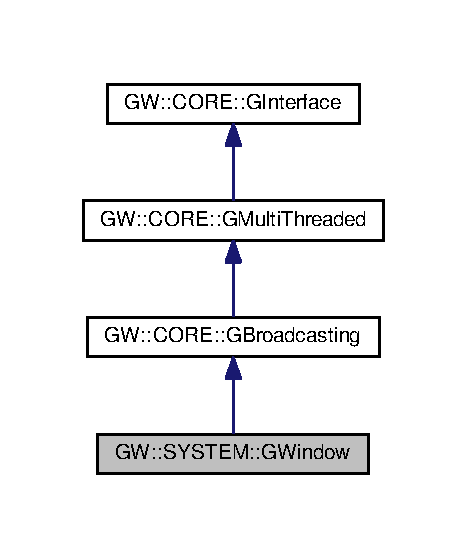
\includegraphics[width=224pt]{classGW_1_1SYSTEM_1_1GWindow__inherit__graph}
\end{center}
\end{figure}


Collaboration diagram for GW\+:\+:S\+Y\+S\+T\+EM\+:\+:G\+Window\+:
\nopagebreak
\begin{figure}[H]
\begin{center}
\leavevmode
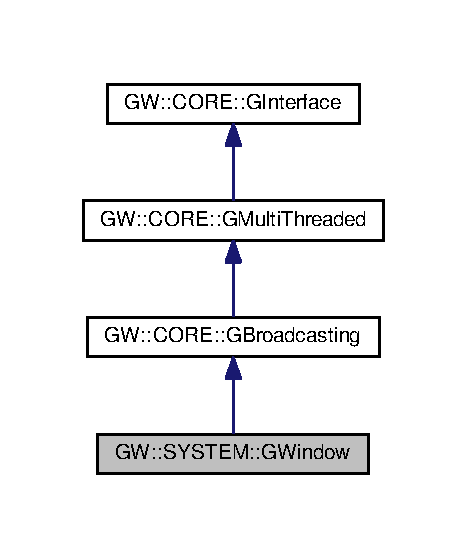
\includegraphics[width=224pt]{classGW_1_1SYSTEM_1_1GWindow__coll__graph}
\end{center}
\end{figure}
\subsection*{Public Member Functions}
\begin{DoxyCompactItemize}
\item 
virtual \hyperlink{namespaceGW_a67a839e3df7ea8a5c5686613a7a3de21}{G\+Return} \hyperlink{classGW_1_1SYSTEM_1_1GWindow_a402b550212d77f19638ef1a1db9ad397}{Open\+Window} ()=0
\begin{DoxyCompactList}\small\item\em Initializes a window handle and displays a window. \end{DoxyCompactList}\item 
virtual \hyperlink{namespaceGW_a67a839e3df7ea8a5c5686613a7a3de21}{G\+Return} \hyperlink{classGW_1_1SYSTEM_1_1GWindow_a6c7db60db04436ac21cba3147f287e84}{Process\+Window\+Events} ()=0
\begin{DoxyCompactList}\small\item\em Flushes and processes all messages from the window\textquotesingle{}s event queue. \end{DoxyCompactList}\item 
virtual \hyperlink{namespaceGW_a67a839e3df7ea8a5c5686613a7a3de21}{G\+Return} \hyperlink{classGW_1_1SYSTEM_1_1GWindow_a113350a164370d30932a0476f00e4ea9}{Reconfigure\+Window} (int \+\_\+x, int \+\_\+y, int \+\_\+width, int \+\_\+height, \hyperlink{namespaceGW_1_1SYSTEM_ad117891e556631f842625c348d36a071}{G\+Window\+Style} \+\_\+style)=0
\begin{DoxyCompactList}\small\item\em Gives the currently opened window the specified size, position and style. \end{DoxyCompactList}\item 
virtual \hyperlink{namespaceGW_a67a839e3df7ea8a5c5686613a7a3de21}{G\+Return} \hyperlink{classGW_1_1SYSTEM_1_1GWindow_a9fc043b893f26c35e6ba965adcc17edb}{Move\+Window} (int \+\_\+x, int \+\_\+y)=0
\begin{DoxyCompactList}\small\item\em Repositions the currently opened window to the specified x and y pixels on screen. \end{DoxyCompactList}\item 
virtual \hyperlink{namespaceGW_a67a839e3df7ea8a5c5686613a7a3de21}{G\+Return} \hyperlink{classGW_1_1SYSTEM_1_1GWindow_a92633707248f32e4c166f27f03690d6d}{Resize\+Window} (int \+\_\+width, int \+\_\+height)=0
\begin{DoxyCompactList}\small\item\em Resizes the currently opened window to the specified width and height. \end{DoxyCompactList}\item 
virtual \hyperlink{namespaceGW_a67a839e3df7ea8a5c5686613a7a3de21}{G\+Return} \hyperlink{classGW_1_1SYSTEM_1_1GWindow_a06b5f092e742baca82a0bfc2cbaef153}{Maximize} ()=0
\begin{DoxyCompactList}\small\item\em Resizes the currently opened window to the native maximum resolution. \end{DoxyCompactList}\item 
virtual \hyperlink{namespaceGW_a67a839e3df7ea8a5c5686613a7a3de21}{G\+Return} \hyperlink{classGW_1_1SYSTEM_1_1GWindow_a2cced61a323dac10535904c3899563d8}{Minimize} ()=0
\begin{DoxyCompactList}\small\item\em Minimizes the currently opened window. \end{DoxyCompactList}\item 
virtual \hyperlink{namespaceGW_a67a839e3df7ea8a5c5686613a7a3de21}{G\+Return} \hyperlink{classGW_1_1SYSTEM_1_1GWindow_a21533c58e920d347c377ebdaa6d2b76f}{Change\+Window\+Style} (\hyperlink{namespaceGW_1_1SYSTEM_ad117891e556631f842625c348d36a071}{G\+Window\+Style} \+\_\+style)=0
\begin{DoxyCompactList}\small\item\em Sets the currently opened window\textquotesingle{}s style to the specified style. \end{DoxyCompactList}\item 
virtual int \hyperlink{classGW_1_1SYSTEM_1_1GWindow_a5afa3ef5f507b1dcb041d57280378e62}{Get\+Width} ()=0
\begin{DoxyCompactList}\small\item\em Returns the width in pixels of the currently opened window. \end{DoxyCompactList}\item 
virtual int \hyperlink{classGW_1_1SYSTEM_1_1GWindow_a159a5aca2f2a77b756591ff29574cdc9}{Get\+Height} ()=0
\begin{DoxyCompactList}\small\item\em Returns the height in pixels of the currently opened window. \end{DoxyCompactList}\item 
virtual int \hyperlink{classGW_1_1SYSTEM_1_1GWindow_a1a4bdd7bb12a39d5bbaae53f1e180d91}{Get\+Client\+Width} ()=0
\begin{DoxyCompactList}\small\item\em Returns the client width in pixels of the currently opened window. \end{DoxyCompactList}\item 
virtual int \hyperlink{classGW_1_1SYSTEM_1_1GWindow_ac0a08847a67fbb588f6a851007f465f0}{Get\+Client\+Height} ()=0
\begin{DoxyCompactList}\small\item\em Returns the client height in pixels of the currently opened window. \end{DoxyCompactList}\item 
virtual int \hyperlink{classGW_1_1SYSTEM_1_1GWindow_a085fd92d1a4f5cb131ca405dc69d28ea}{GetX} ()=0
\begin{DoxyCompactList}\small\item\em Returns the X position in pixels of the currently opened window. \end{DoxyCompactList}\item 
virtual int \hyperlink{classGW_1_1SYSTEM_1_1GWindow_a37525397599eb9fc9fced0fe3a69fc04}{GetY} ()=0
\begin{DoxyCompactList}\small\item\em Returns the Y position in pixels of the currently opened window. \end{DoxyCompactList}\item 
virtual \hyperlink{namespaceGW_a67a839e3df7ea8a5c5686613a7a3de21}{G\+Return} \hyperlink{classGW_1_1SYSTEM_1_1GWindow_ac80bfaba809d5eb54d6a11b11deddeb7}{Get\+Client\+Top\+Left} (unsigned int \&\+\_\+outX, unsigned int \&\+\_\+outY)=0
\begin{DoxyCompactList}\small\item\em Gets the location of the top-\/left pixel of the opened window\textquotesingle{}s client area. \end{DoxyCompactList}\item 
virtual void $\ast$ \hyperlink{classGW_1_1SYSTEM_1_1GWindow_aa3cc3af1805ac9573424f8815420e9c5}{Get\+Window\+Handle} ()=0
\begin{DoxyCompactList}\small\item\em Returns the platform specific window handle to the currently opened window. \end{DoxyCompactList}\item 
virtual bool \hyperlink{classGW_1_1SYSTEM_1_1GWindow_acf85e727f26eeeeb3e006947c45d04a3}{Is\+Fullscreen} ()=0
\begin{DoxyCompactList}\small\item\em Returns a bool specifying whether or not the currently opened window is fullscreen. \end{DoxyCompactList}\end{DoxyCompactItemize}


\subsection{Detailed Description}
A thread-\/safe window creation and management library. 

This library is used to create, move, resize, and destroy a window. Methods exist to query information from the window as well. The window is also a broadcaster, meaning a G\+Listener can be written to receive events from it. 

\subsection{Member Function Documentation}
\index{G\+W\+::\+S\+Y\+S\+T\+E\+M\+::\+G\+Window@{G\+W\+::\+S\+Y\+S\+T\+E\+M\+::\+G\+Window}!Change\+Window\+Style@{Change\+Window\+Style}}
\index{Change\+Window\+Style@{Change\+Window\+Style}!G\+W\+::\+S\+Y\+S\+T\+E\+M\+::\+G\+Window@{G\+W\+::\+S\+Y\+S\+T\+E\+M\+::\+G\+Window}}
\subsubsection[{\texorpdfstring{Change\+Window\+Style(\+G\+Window\+Style \+\_\+style)=0}{ChangeWindowStyle(GWindowStyle _style)=0}}]{\setlength{\rightskip}{0pt plus 5cm}virtual {\bf G\+Return} G\+W\+::\+S\+Y\+S\+T\+E\+M\+::\+G\+Window\+::\+Change\+Window\+Style (
\begin{DoxyParamCaption}
\item[{{\bf G\+Window\+Style}}]{\+\_\+style}
\end{DoxyParamCaption}
)\hspace{0.3cm}{\ttfamily [pure virtual]}}\hypertarget{classGW_1_1SYSTEM_1_1GWindow_a21533c58e920d347c377ebdaa6d2b76f}{}\label{classGW_1_1SYSTEM_1_1GWindow_a21533c58e920d347c377ebdaa6d2b76f}


Sets the currently opened window\textquotesingle{}s style to the specified style. 

G\+Window\+Style will be overwritten and the window resized or moved accordingly.


\begin{DoxyParams}[1]{Parameters}
\mbox{\tt in}  & {\em \+\_\+style} & The G\+Window\+Style to change the window to.\\
\hline
\end{DoxyParams}

\begin{DoxyRetVals}{Return values}
{\em S\+U\+C\+C\+E\+SS} & The window style was successfully changed. \\
\hline
{\em R\+E\+D\+U\+N\+D\+A\+N\+T\+\_\+\+O\+P\+E\+R\+A\+T\+I\+ON} & No window exists to change. \\
\hline
\end{DoxyRetVals}
\index{G\+W\+::\+S\+Y\+S\+T\+E\+M\+::\+G\+Window@{G\+W\+::\+S\+Y\+S\+T\+E\+M\+::\+G\+Window}!Get\+Client\+Height@{Get\+Client\+Height}}
\index{Get\+Client\+Height@{Get\+Client\+Height}!G\+W\+::\+S\+Y\+S\+T\+E\+M\+::\+G\+Window@{G\+W\+::\+S\+Y\+S\+T\+E\+M\+::\+G\+Window}}
\subsubsection[{\texorpdfstring{Get\+Client\+Height()=0}{GetClientHeight()=0}}]{\setlength{\rightskip}{0pt plus 5cm}virtual int G\+W\+::\+S\+Y\+S\+T\+E\+M\+::\+G\+Window\+::\+Get\+Client\+Height (
\begin{DoxyParamCaption}
{}
\end{DoxyParamCaption}
)\hspace{0.3cm}{\ttfamily [pure virtual]}}\hypertarget{classGW_1_1SYSTEM_1_1GWindow_ac0a08847a67fbb588f6a851007f465f0}{}\label{classGW_1_1SYSTEM_1_1GWindow_ac0a08847a67fbb588f6a851007f465f0}


Returns the client height in pixels of the currently opened window. 


\begin{DoxyRetVals}{Return values}
{\em 0} & The window is minimized. \\
\hline
{\em -\/1} & No window exists to query size from. \\
\hline
{\em else} & Height was successfully queried and returned. \\
\hline
\end{DoxyRetVals}
\index{G\+W\+::\+S\+Y\+S\+T\+E\+M\+::\+G\+Window@{G\+W\+::\+S\+Y\+S\+T\+E\+M\+::\+G\+Window}!Get\+Client\+Top\+Left@{Get\+Client\+Top\+Left}}
\index{Get\+Client\+Top\+Left@{Get\+Client\+Top\+Left}!G\+W\+::\+S\+Y\+S\+T\+E\+M\+::\+G\+Window@{G\+W\+::\+S\+Y\+S\+T\+E\+M\+::\+G\+Window}}
\subsubsection[{\texorpdfstring{Get\+Client\+Top\+Left(unsigned int \&\+\_\+out\+X, unsigned int \&\+\_\+out\+Y)=0}{GetClientTopLeft(unsigned int &_outX, unsigned int &_outY)=0}}]{\setlength{\rightskip}{0pt plus 5cm}virtual {\bf G\+Return} G\+W\+::\+S\+Y\+S\+T\+E\+M\+::\+G\+Window\+::\+Get\+Client\+Top\+Left (
\begin{DoxyParamCaption}
\item[{unsigned int \&}]{\+\_\+outX, }
\item[{unsigned int \&}]{\+\_\+outY}
\end{DoxyParamCaption}
)\hspace{0.3cm}{\ttfamily [pure virtual]}}\hypertarget{classGW_1_1SYSTEM_1_1GWindow_ac80bfaba809d5eb54d6a11b11deddeb7}{}\label{classGW_1_1SYSTEM_1_1GWindow_ac80bfaba809d5eb54d6a11b11deddeb7}


Gets the location of the top-\/left pixel of the opened window\textquotesingle{}s client area. 


\begin{DoxyParams}[1]{Parameters}
\mbox{\tt out}  & {\em \+\_\+outX} & Will contain the X location of the top-\/left pixel. \\
\hline
\mbox{\tt out}  & {\em \+\_\+outY} & Will contain the Y location of the top-\/left pixel.\\
\hline
\end{DoxyParams}

\begin{DoxyRetVals}{Return values}
{\em -\/1} & No window exists to query position from. \\
\hline
{\em else} & Position was successfully queried and returned. \\
\hline
\end{DoxyRetVals}
\index{G\+W\+::\+S\+Y\+S\+T\+E\+M\+::\+G\+Window@{G\+W\+::\+S\+Y\+S\+T\+E\+M\+::\+G\+Window}!Get\+Client\+Width@{Get\+Client\+Width}}
\index{Get\+Client\+Width@{Get\+Client\+Width}!G\+W\+::\+S\+Y\+S\+T\+E\+M\+::\+G\+Window@{G\+W\+::\+S\+Y\+S\+T\+E\+M\+::\+G\+Window}}
\subsubsection[{\texorpdfstring{Get\+Client\+Width()=0}{GetClientWidth()=0}}]{\setlength{\rightskip}{0pt plus 5cm}virtual int G\+W\+::\+S\+Y\+S\+T\+E\+M\+::\+G\+Window\+::\+Get\+Client\+Width (
\begin{DoxyParamCaption}
{}
\end{DoxyParamCaption}
)\hspace{0.3cm}{\ttfamily [pure virtual]}}\hypertarget{classGW_1_1SYSTEM_1_1GWindow_a1a4bdd7bb12a39d5bbaae53f1e180d91}{}\label{classGW_1_1SYSTEM_1_1GWindow_a1a4bdd7bb12a39d5bbaae53f1e180d91}


Returns the client width in pixels of the currently opened window. 

Client height is the height of the window\textquotesingle{}s drawable area.


\begin{DoxyRetVals}{Return values}
{\em 0} & The window is minimized. \\
\hline
{\em -\/1} & No window exists to query size from. \\
\hline
{\em else} & Width was successfully queried and returned. \\
\hline
\end{DoxyRetVals}
\index{G\+W\+::\+S\+Y\+S\+T\+E\+M\+::\+G\+Window@{G\+W\+::\+S\+Y\+S\+T\+E\+M\+::\+G\+Window}!Get\+Height@{Get\+Height}}
\index{Get\+Height@{Get\+Height}!G\+W\+::\+S\+Y\+S\+T\+E\+M\+::\+G\+Window@{G\+W\+::\+S\+Y\+S\+T\+E\+M\+::\+G\+Window}}
\subsubsection[{\texorpdfstring{Get\+Height()=0}{GetHeight()=0}}]{\setlength{\rightskip}{0pt plus 5cm}virtual int G\+W\+::\+S\+Y\+S\+T\+E\+M\+::\+G\+Window\+::\+Get\+Height (
\begin{DoxyParamCaption}
{}
\end{DoxyParamCaption}
)\hspace{0.3cm}{\ttfamily [pure virtual]}}\hypertarget{classGW_1_1SYSTEM_1_1GWindow_a159a5aca2f2a77b756591ff29574cdc9}{}\label{classGW_1_1SYSTEM_1_1GWindow_a159a5aca2f2a77b756591ff29574cdc9}


Returns the height in pixels of the currently opened window. 

Client width is the width of the window\textquotesingle{}s drawable area.


\begin{DoxyRetVals}{Return values}
{\em 0} & The window is minimized. \\
\hline
{\em -\/1} & No window exists to query size from. \\
\hline
{\em else} & Height was successfully queried and returned. \\
\hline
\end{DoxyRetVals}
\index{G\+W\+::\+S\+Y\+S\+T\+E\+M\+::\+G\+Window@{G\+W\+::\+S\+Y\+S\+T\+E\+M\+::\+G\+Window}!Get\+Width@{Get\+Width}}
\index{Get\+Width@{Get\+Width}!G\+W\+::\+S\+Y\+S\+T\+E\+M\+::\+G\+Window@{G\+W\+::\+S\+Y\+S\+T\+E\+M\+::\+G\+Window}}
\subsubsection[{\texorpdfstring{Get\+Width()=0}{GetWidth()=0}}]{\setlength{\rightskip}{0pt plus 5cm}virtual int G\+W\+::\+S\+Y\+S\+T\+E\+M\+::\+G\+Window\+::\+Get\+Width (
\begin{DoxyParamCaption}
{}
\end{DoxyParamCaption}
)\hspace{0.3cm}{\ttfamily [pure virtual]}}\hypertarget{classGW_1_1SYSTEM_1_1GWindow_a5afa3ef5f507b1dcb041d57280378e62}{}\label{classGW_1_1SYSTEM_1_1GWindow_a5afa3ef5f507b1dcb041d57280378e62}


Returns the width in pixels of the currently opened window. 


\begin{DoxyRetVals}{Return values}
{\em 0} & The window is minimized. \\
\hline
{\em -\/1} & No window exists to query size from. \\
\hline
{\em else} & Width was successfully queried and returned. \\
\hline
\end{DoxyRetVals}
\index{G\+W\+::\+S\+Y\+S\+T\+E\+M\+::\+G\+Window@{G\+W\+::\+S\+Y\+S\+T\+E\+M\+::\+G\+Window}!Get\+Window\+Handle@{Get\+Window\+Handle}}
\index{Get\+Window\+Handle@{Get\+Window\+Handle}!G\+W\+::\+S\+Y\+S\+T\+E\+M\+::\+G\+Window@{G\+W\+::\+S\+Y\+S\+T\+E\+M\+::\+G\+Window}}
\subsubsection[{\texorpdfstring{Get\+Window\+Handle()=0}{GetWindowHandle()=0}}]{\setlength{\rightskip}{0pt plus 5cm}virtual void$\ast$ G\+W\+::\+S\+Y\+S\+T\+E\+M\+::\+G\+Window\+::\+Get\+Window\+Handle (
\begin{DoxyParamCaption}
{}
\end{DoxyParamCaption}
)\hspace{0.3cm}{\ttfamily [pure virtual]}}\hypertarget{classGW_1_1SYSTEM_1_1GWindow_aa3cc3af1805ac9573424f8815420e9c5}{}\label{classGW_1_1SYSTEM_1_1GWindow_aa3cc3af1805ac9573424f8815420e9c5}


Returns the platform specific window handle to the currently opened window. 

On Windows the void$\ast$ is an H\+W\+ND, on Linux a \hyperlink{structGW_1_1SYSTEM_1_1LINUX__WINDOW}{L\+I\+N\+U\+X\+\_\+\+W\+I\+N\+D\+OW}, and on Mac an N\+S\+Window. Methods exist to query window information right from these handles.


\begin{DoxyRetVals}{Return values}
{\em void$\ast$} & The void$\ast$ data to the window handle. \\
\hline
\end{DoxyRetVals}
\index{G\+W\+::\+S\+Y\+S\+T\+E\+M\+::\+G\+Window@{G\+W\+::\+S\+Y\+S\+T\+E\+M\+::\+G\+Window}!GetX@{GetX}}
\index{GetX@{GetX}!G\+W\+::\+S\+Y\+S\+T\+E\+M\+::\+G\+Window@{G\+W\+::\+S\+Y\+S\+T\+E\+M\+::\+G\+Window}}
\subsubsection[{\texorpdfstring{Get\+X()=0}{GetX()=0}}]{\setlength{\rightskip}{0pt plus 5cm}virtual int G\+W\+::\+S\+Y\+S\+T\+E\+M\+::\+G\+Window\+::\+GetX (
\begin{DoxyParamCaption}
{}
\end{DoxyParamCaption}
)\hspace{0.3cm}{\ttfamily [pure virtual]}}\hypertarget{classGW_1_1SYSTEM_1_1GWindow_a085fd92d1a4f5cb131ca405dc69d28ea}{}\label{classGW_1_1SYSTEM_1_1GWindow_a085fd92d1a4f5cb131ca405dc69d28ea}


Returns the X position in pixels of the currently opened window. 


\begin{DoxyRetVals}{Return values}
{\em -\/1} & No window exists to query position from. \\
\hline
{\em else} & X position was successfully queried and returned. \\
\hline
\end{DoxyRetVals}
\index{G\+W\+::\+S\+Y\+S\+T\+E\+M\+::\+G\+Window@{G\+W\+::\+S\+Y\+S\+T\+E\+M\+::\+G\+Window}!GetY@{GetY}}
\index{GetY@{GetY}!G\+W\+::\+S\+Y\+S\+T\+E\+M\+::\+G\+Window@{G\+W\+::\+S\+Y\+S\+T\+E\+M\+::\+G\+Window}}
\subsubsection[{\texorpdfstring{Get\+Y()=0}{GetY()=0}}]{\setlength{\rightskip}{0pt plus 5cm}virtual int G\+W\+::\+S\+Y\+S\+T\+E\+M\+::\+G\+Window\+::\+GetY (
\begin{DoxyParamCaption}
{}
\end{DoxyParamCaption}
)\hspace{0.3cm}{\ttfamily [pure virtual]}}\hypertarget{classGW_1_1SYSTEM_1_1GWindow_a37525397599eb9fc9fced0fe3a69fc04}{}\label{classGW_1_1SYSTEM_1_1GWindow_a37525397599eb9fc9fced0fe3a69fc04}


Returns the Y position in pixels of the currently opened window. 


\begin{DoxyRetVals}{Return values}
{\em -\/1} & No window exists to query position from. \\
\hline
{\em else} & Y position was successfully queried and returned. \\
\hline
\end{DoxyRetVals}
\index{G\+W\+::\+S\+Y\+S\+T\+E\+M\+::\+G\+Window@{G\+W\+::\+S\+Y\+S\+T\+E\+M\+::\+G\+Window}!Is\+Fullscreen@{Is\+Fullscreen}}
\index{Is\+Fullscreen@{Is\+Fullscreen}!G\+W\+::\+S\+Y\+S\+T\+E\+M\+::\+G\+Window@{G\+W\+::\+S\+Y\+S\+T\+E\+M\+::\+G\+Window}}
\subsubsection[{\texorpdfstring{Is\+Fullscreen()=0}{IsFullscreen()=0}}]{\setlength{\rightskip}{0pt plus 5cm}virtual bool G\+W\+::\+S\+Y\+S\+T\+E\+M\+::\+G\+Window\+::\+Is\+Fullscreen (
\begin{DoxyParamCaption}
{}
\end{DoxyParamCaption}
)\hspace{0.3cm}{\ttfamily [pure virtual]}}\hypertarget{classGW_1_1SYSTEM_1_1GWindow_acf85e727f26eeeeb3e006947c45d04a3}{}\label{classGW_1_1SYSTEM_1_1GWindow_acf85e727f26eeeeb3e006947c45d04a3}


Returns a bool specifying whether or not the currently opened window is fullscreen. 


\begin{DoxyRetVals}{Return values}
{\em true} & The window is fullscreen. \\
\hline
{\em false} & The window is not fullscreen. \\
\hline
\end{DoxyRetVals}
\index{G\+W\+::\+S\+Y\+S\+T\+E\+M\+::\+G\+Window@{G\+W\+::\+S\+Y\+S\+T\+E\+M\+::\+G\+Window}!Maximize@{Maximize}}
\index{Maximize@{Maximize}!G\+W\+::\+S\+Y\+S\+T\+E\+M\+::\+G\+Window@{G\+W\+::\+S\+Y\+S\+T\+E\+M\+::\+G\+Window}}
\subsubsection[{\texorpdfstring{Maximize()=0}{Maximize()=0}}]{\setlength{\rightskip}{0pt plus 5cm}virtual {\bf G\+Return} G\+W\+::\+S\+Y\+S\+T\+E\+M\+::\+G\+Window\+::\+Maximize (
\begin{DoxyParamCaption}
{}
\end{DoxyParamCaption}
)\hspace{0.3cm}{\ttfamily [pure virtual]}}\hypertarget{classGW_1_1SYSTEM_1_1GWindow_a06b5f092e742baca82a0bfc2cbaef153}{}\label{classGW_1_1SYSTEM_1_1GWindow_a06b5f092e742baca82a0bfc2cbaef153}


Resizes the currently opened window to the native maximum resolution. 

G\+Window\+Style will be overwritten to be the fullscreen version if it is not already.


\begin{DoxyRetVals}{Return values}
{\em S\+U\+C\+C\+E\+SS} & The window was successfully maximized. \\
\hline
{\em R\+E\+D\+U\+N\+D\+A\+N\+T\+\_\+\+O\+P\+E\+R\+A\+T\+I\+ON} & No window exists to maximize. \\
\hline
\end{DoxyRetVals}
\index{G\+W\+::\+S\+Y\+S\+T\+E\+M\+::\+G\+Window@{G\+W\+::\+S\+Y\+S\+T\+E\+M\+::\+G\+Window}!Minimize@{Minimize}}
\index{Minimize@{Minimize}!G\+W\+::\+S\+Y\+S\+T\+E\+M\+::\+G\+Window@{G\+W\+::\+S\+Y\+S\+T\+E\+M\+::\+G\+Window}}
\subsubsection[{\texorpdfstring{Minimize()=0}{Minimize()=0}}]{\setlength{\rightskip}{0pt plus 5cm}virtual {\bf G\+Return} G\+W\+::\+S\+Y\+S\+T\+E\+M\+::\+G\+Window\+::\+Minimize (
\begin{DoxyParamCaption}
{}
\end{DoxyParamCaption}
)\hspace{0.3cm}{\ttfamily [pure virtual]}}\hypertarget{classGW_1_1SYSTEM_1_1GWindow_a2cced61a323dac10535904c3899563d8}{}\label{classGW_1_1SYSTEM_1_1GWindow_a2cced61a323dac10535904c3899563d8}


Minimizes the currently opened window. 

G\+Window\+Style will be overwritten to be the minimized style if it is not already.


\begin{DoxyRetVals}{Return values}
{\em S\+U\+C\+C\+E\+SS} & The window was successfully minimized. \\
\hline
{\em R\+E\+D\+U\+N\+D\+A\+N\+T\+\_\+\+O\+P\+E\+R\+A\+T\+I\+ON} & No window exists to minimize or window is already maximized. \\
\hline
\end{DoxyRetVals}
\index{G\+W\+::\+S\+Y\+S\+T\+E\+M\+::\+G\+Window@{G\+W\+::\+S\+Y\+S\+T\+E\+M\+::\+G\+Window}!Move\+Window@{Move\+Window}}
\index{Move\+Window@{Move\+Window}!G\+W\+::\+S\+Y\+S\+T\+E\+M\+::\+G\+Window@{G\+W\+::\+S\+Y\+S\+T\+E\+M\+::\+G\+Window}}
\subsubsection[{\texorpdfstring{Move\+Window(int \+\_\+x, int \+\_\+y)=0}{MoveWindow(int _x, int _y)=0}}]{\setlength{\rightskip}{0pt plus 5cm}virtual {\bf G\+Return} G\+W\+::\+S\+Y\+S\+T\+E\+M\+::\+G\+Window\+::\+Move\+Window (
\begin{DoxyParamCaption}
\item[{int}]{\+\_\+x, }
\item[{int}]{\+\_\+y}
\end{DoxyParamCaption}
)\hspace{0.3cm}{\ttfamily [pure virtual]}}\hypertarget{classGW_1_1SYSTEM_1_1GWindow_a9fc043b893f26c35e6ba965adcc17edb}{}\label{classGW_1_1SYSTEM_1_1GWindow_a9fc043b893f26c35e6ba965adcc17edb}


Repositions the currently opened window to the specified x and y pixels on screen. 

If position parameters are less than 0 then 0 will be used. If position parameters are greater than native resoultion, maximum native resolution parameters will be used.


\begin{DoxyParams}[1]{Parameters}
\mbox{\tt in}  & {\em \+\_\+x} & The x position on screen to move the window to. \\
\hline
\mbox{\tt in}  & {\em \+\_\+y} & The y position on screen to move the window to.\\
\hline
\end{DoxyParams}

\begin{DoxyRetVals}{Return values}
{\em S\+U\+C\+C\+E\+SS} & The window was successfully moved. \\
\hline
{\em I\+N\+V\+A\+L\+I\+D\+\_\+\+A\+R\+G\+U\+M\+E\+NT} & The style passed in is invalid \\
\hline
{\em R\+E\+D\+U\+N\+D\+A\+N\+T\+\_\+\+O\+P\+E\+R\+A\+T\+I\+ON} & No window exists to move. \\
\hline
\end{DoxyRetVals}
\index{G\+W\+::\+S\+Y\+S\+T\+E\+M\+::\+G\+Window@{G\+W\+::\+S\+Y\+S\+T\+E\+M\+::\+G\+Window}!Open\+Window@{Open\+Window}}
\index{Open\+Window@{Open\+Window}!G\+W\+::\+S\+Y\+S\+T\+E\+M\+::\+G\+Window@{G\+W\+::\+S\+Y\+S\+T\+E\+M\+::\+G\+Window}}
\subsubsection[{\texorpdfstring{Open\+Window()=0}{OpenWindow()=0}}]{\setlength{\rightskip}{0pt plus 5cm}virtual {\bf G\+Return} G\+W\+::\+S\+Y\+S\+T\+E\+M\+::\+G\+Window\+::\+Open\+Window (
\begin{DoxyParamCaption}
{}
\end{DoxyParamCaption}
)\hspace{0.3cm}{\ttfamily [pure virtual]}}\hypertarget{classGW_1_1SYSTEM_1_1GWindow_a402b550212d77f19638ef1a1db9ad397}{}\label{classGW_1_1SYSTEM_1_1GWindow_a402b550212d77f19638ef1a1db9ad397}


Initializes a window handle and displays a window. 

The window is opened with the size, position and style specified in the parameters passed into the Create\+G\+Window function. Parameters were checked for invalid values during the initialization of the window after creation, so it is assumed the window has valid parameters before this function is called.


\begin{DoxyRetVals}{Return values}
{\em S\+U\+C\+C\+E\+SS} & The window was successfully created and displayed. \\
\hline
{\em R\+E\+D\+U\+N\+D\+A\+N\+T\+\_\+\+O\+P\+E\+R\+A\+T\+I\+ON} & The \hyperlink{classGW_1_1SYSTEM_1_1GWindow}{G\+Window} object already has a window open \\
\hline
{\em F\+A\+I\+L\+U\+RE} & The window could not be created. \\
\hline
\end{DoxyRetVals}
\index{G\+W\+::\+S\+Y\+S\+T\+E\+M\+::\+G\+Window@{G\+W\+::\+S\+Y\+S\+T\+E\+M\+::\+G\+Window}!Process\+Window\+Events@{Process\+Window\+Events}}
\index{Process\+Window\+Events@{Process\+Window\+Events}!G\+W\+::\+S\+Y\+S\+T\+E\+M\+::\+G\+Window@{G\+W\+::\+S\+Y\+S\+T\+E\+M\+::\+G\+Window}}
\subsubsection[{\texorpdfstring{Process\+Window\+Events()=0}{ProcessWindowEvents()=0}}]{\setlength{\rightskip}{0pt plus 5cm}virtual {\bf G\+Return} G\+W\+::\+S\+Y\+S\+T\+E\+M\+::\+G\+Window\+::\+Process\+Window\+Events (
\begin{DoxyParamCaption}
{}
\end{DoxyParamCaption}
)\hspace{0.3cm}{\ttfamily [pure virtual]}}\hypertarget{classGW_1_1SYSTEM_1_1GWindow_a6c7db60db04436ac21cba3147f287e84}{}\label{classGW_1_1SYSTEM_1_1GWindow_a6c7db60db04436ac21cba3147f287e84}


Flushes and processes all messages from the window\textquotesingle{}s event queue. 

This function is meant to be called once a frame in an application\textquotesingle{}s main loop. This function will break when all waiting messages have been processed and the event queue is empty.


\begin{DoxyRetVals}{Return values}
{\em S\+U\+C\+C\+E\+SS} & The messages were successfully processed and removed. \\
\hline
{\em R\+E\+D\+U\+N\+D\+A\+N\+T\+\_\+\+O\+P\+E\+R\+A\+T\+I\+ON} & No window exists process. \\
\hline
\end{DoxyRetVals}
\index{G\+W\+::\+S\+Y\+S\+T\+E\+M\+::\+G\+Window@{G\+W\+::\+S\+Y\+S\+T\+E\+M\+::\+G\+Window}!Reconfigure\+Window@{Reconfigure\+Window}}
\index{Reconfigure\+Window@{Reconfigure\+Window}!G\+W\+::\+S\+Y\+S\+T\+E\+M\+::\+G\+Window@{G\+W\+::\+S\+Y\+S\+T\+E\+M\+::\+G\+Window}}
\subsubsection[{\texorpdfstring{Reconfigure\+Window(int \+\_\+x, int \+\_\+y, int \+\_\+width, int \+\_\+height, G\+Window\+Style \+\_\+style)=0}{ReconfigureWindow(int _x, int _y, int _width, int _height, GWindowStyle _style)=0}}]{\setlength{\rightskip}{0pt plus 5cm}virtual {\bf G\+Return} G\+W\+::\+S\+Y\+S\+T\+E\+M\+::\+G\+Window\+::\+Reconfigure\+Window (
\begin{DoxyParamCaption}
\item[{int}]{\+\_\+x, }
\item[{int}]{\+\_\+y, }
\item[{int}]{\+\_\+width, }
\item[{int}]{\+\_\+height, }
\item[{{\bf G\+Window\+Style}}]{\+\_\+style}
\end{DoxyParamCaption}
)\hspace{0.3cm}{\ttfamily [pure virtual]}}\hypertarget{classGW_1_1SYSTEM_1_1GWindow_a113350a164370d30932a0476f00e4ea9}{}\label{classGW_1_1SYSTEM_1_1GWindow_a113350a164370d30932a0476f00e4ea9}


Gives the currently opened window the specified size, position and style. 

If width and height are equal to or greater than the native resolution, the passed in G\+Window\+Style will be overwritten to be the fullscreen version if it is not already. If position parameters are less than 0 then 0 will be used. If position parameters are greater than native resoultion, maximum native resolution parameters will be used.


\begin{DoxyParams}[1]{Parameters}
\mbox{\tt in}  & {\em \+\_\+x} & The x position on screen to move the window to. \\
\hline
\mbox{\tt in}  & {\em \+\_\+y} & The y position on screen to move the window to. \\
\hline
\mbox{\tt in}  & {\em \+\_\+width} & The width to give the window. \\
\hline
\mbox{\tt in}  & {\em \+\_\+height} & The height to give the window. \\
\hline
\mbox{\tt in}  & {\em \+\_\+style} & The style to give to the window. (see G\+Window\+Style for style options)\\
\hline
\end{DoxyParams}

\begin{DoxyRetVals}{Return values}
{\em S\+U\+C\+C\+E\+SS} & The window successfully had its attributes changed. \\
\hline
{\em I\+N\+V\+A\+L\+I\+D\+\_\+\+A\+R\+G\+U\+M\+E\+NT} & One of the size parameters are outside the limits of the hardware. \\
\hline
{\em R\+E\+D\+U\+N\+D\+A\+N\+T\+\_\+\+O\+P\+E\+R\+A\+T\+I\+ON} & No window exists to edit. \\
\hline
\end{DoxyRetVals}
\index{G\+W\+::\+S\+Y\+S\+T\+E\+M\+::\+G\+Window@{G\+W\+::\+S\+Y\+S\+T\+E\+M\+::\+G\+Window}!Resize\+Window@{Resize\+Window}}
\index{Resize\+Window@{Resize\+Window}!G\+W\+::\+S\+Y\+S\+T\+E\+M\+::\+G\+Window@{G\+W\+::\+S\+Y\+S\+T\+E\+M\+::\+G\+Window}}
\subsubsection[{\texorpdfstring{Resize\+Window(int \+\_\+width, int \+\_\+height)=0}{ResizeWindow(int _width, int _height)=0}}]{\setlength{\rightskip}{0pt plus 5cm}virtual {\bf G\+Return} G\+W\+::\+S\+Y\+S\+T\+E\+M\+::\+G\+Window\+::\+Resize\+Window (
\begin{DoxyParamCaption}
\item[{int}]{\+\_\+width, }
\item[{int}]{\+\_\+height}
\end{DoxyParamCaption}
)\hspace{0.3cm}{\ttfamily [pure virtual]}}\hypertarget{classGW_1_1SYSTEM_1_1GWindow_a92633707248f32e4c166f27f03690d6d}{}\label{classGW_1_1SYSTEM_1_1GWindow_a92633707248f32e4c166f27f03690d6d}


Resizes the currently opened window to the specified width and height. 

If width and height are greater than the native resolution, the G\+Window\+Style will be overwritten to be the fullscreen version if it is not already. If position parameters are less than 0 then 0 will be used. If position parameters are greater than native resoultion, maximum native resolution parameters will be used.


\begin{DoxyParams}[1]{Parameters}
\mbox{\tt in}  & {\em \+\_\+x} & The width to resize the window to. \\
\hline
\mbox{\tt in}  & {\em \+\_\+y} & The height to resize the window to.\\
\hline
\end{DoxyParams}

\begin{DoxyRetVals}{Return values}
{\em S\+U\+C\+C\+E\+SS} & The window was successfully resized. \\
\hline
{\em I\+N\+V\+A\+L\+I\+D\+\_\+\+A\+R\+G\+U\+M\+E\+NT} & One of the size parameters are less than or equal to 0. \\
\hline
{\em R\+E\+D\+U\+N\+D\+A\+N\+T\+\_\+\+O\+P\+E\+R\+A\+T\+I\+ON} & No window exists to resize. \\
\hline
\end{DoxyRetVals}


The documentation for this class was generated from the following file\+:\begin{DoxyCompactItemize}
\item 
Interface/\+G\+\_\+\+System/G\+Window.\+h\end{DoxyCompactItemize}

\hypertarget{structGW_1_1SYSTEM_1_1GWINDOW__EVENT__DATA}{}\section{GW\+::S\+Y\+S\+T\+EM\+::G\+W\+I\+N\+D\+O\+W\+\_\+\+E\+V\+E\+N\+T\+\_\+\+D\+A\+TA Struct Reference}
\label{structGW_1_1SYSTEM_1_1GWINDOW__EVENT__DATA}\index{GW::SYSTEM::GWINDOW\_EVENT\_DATA@{GW::SYSTEM::GWINDOW\_EVENT\_DATA}}


Ensure identical binary padding for structures on all platforms.  




{\ttfamily \#include $<$G\+Window.\+h$>$}

\subsection*{Public Attributes}
\begin{DoxyCompactItemize}
\item 
\mbox{\Hypertarget{structGW_1_1SYSTEM_1_1GWINDOW__EVENT__DATA_a9a3463e7fe90f6c9cb4c4f7d68f62ee1}\label{structGW_1_1SYSTEM_1_1GWINDOW__EVENT__DATA_a9a3463e7fe90f6c9cb4c4f7d68f62ee1}} 
unsigned int {\bfseries event\+Flags}
\item 
\mbox{\Hypertarget{structGW_1_1SYSTEM_1_1GWINDOW__EVENT__DATA_a1bd478c20e20d67fcef4278888f29225}\label{structGW_1_1SYSTEM_1_1GWINDOW__EVENT__DATA_a1bd478c20e20d67fcef4278888f29225}} 
unsigned int {\bfseries height}
\item 
\mbox{\Hypertarget{structGW_1_1SYSTEM_1_1GWINDOW__EVENT__DATA_aedd64cb9564e161fc24a9ea597576dc9}\label{structGW_1_1SYSTEM_1_1GWINDOW__EVENT__DATA_aedd64cb9564e161fc24a9ea597576dc9}} 
unsigned int {\bfseries width}
\item 
\mbox{\Hypertarget{structGW_1_1SYSTEM_1_1GWINDOW__EVENT__DATA_acb671b49c59e58b84d797e5c3ac6deaf}\label{structGW_1_1SYSTEM_1_1GWINDOW__EVENT__DATA_acb671b49c59e58b84d797e5c3ac6deaf}} 
int {\bfseries windowX}
\item 
\mbox{\Hypertarget{structGW_1_1SYSTEM_1_1GWINDOW__EVENT__DATA_aaf455dc933271e4ba81225b8b0433ebc}\label{structGW_1_1SYSTEM_1_1GWINDOW__EVENT__DATA_aaf455dc933271e4ba81225b8b0433ebc}} 
int {\bfseries windowY}
\item 
\mbox{\Hypertarget{structGW_1_1SYSTEM_1_1GWINDOW__EVENT__DATA_a08f52d27570c3cad613dd19fe72a88ac}\label{structGW_1_1SYSTEM_1_1GWINDOW__EVENT__DATA_a08f52d27570c3cad613dd19fe72a88ac}} 
void $\ast$ {\bfseries window\+Handle}
\end{DoxyCompactItemize}


\subsection{Detailed Description}
Ensure identical binary padding for structures on all platforms. 

The documentation for this struct was generated from the following file\+:\begin{DoxyCompactItemize}
\item 
Interface/\+G\+\_\+\+System/G\+Window.\+h\end{DoxyCompactItemize}

\hypertarget{structGW_1_1SYSTEM_1_1LINUX__WINDOW}{}\section{GW\+::S\+Y\+S\+T\+EM\+::L\+I\+N\+U\+X\+\_\+\+W\+I\+N\+D\+OW Struct Reference}
\label{structGW_1_1SYSTEM_1_1LINUX__WINDOW}\index{GW::SYSTEM::LINUX\_WINDOW@{GW::SYSTEM::LINUX\_WINDOW}}


The structure used to pass into Input libraries on Linux.  




{\ttfamily \#include $<$G\+Key\+Defines.\+h$>$}

\subsection*{Public Attributes}
\begin{DoxyCompactItemize}
\item 
\mbox{\Hypertarget{structGW_1_1SYSTEM_1_1LINUX__WINDOW_a9d4ffe1d048716af5f2d1fe3595b6b99}\label{structGW_1_1SYSTEM_1_1LINUX__WINDOW_a9d4ffe1d048716af5f2d1fe3595b6b99}} 
void $\ast$ {\bfseries window}
\item 
\mbox{\Hypertarget{structGW_1_1SYSTEM_1_1LINUX__WINDOW_ae68b93065e8ebd9de010f42ccf688ac5}\label{structGW_1_1SYSTEM_1_1LINUX__WINDOW_ae68b93065e8ebd9de010f42ccf688ac5}} 
void $\ast$ {\bfseries display}
\end{DoxyCompactItemize}


\subsection{Detailed Description}
The structure used to pass into Input libraries on Linux. 

The documentation for this struct was generated from the following file\+:\begin{DoxyCompactItemize}
\item 
Interface/\+G\+\_\+\+System/G\+Key\+Defines.\+h\end{DoxyCompactItemize}

%--- End generated contents ---

% Index
\backmatter
\newpage
\phantomsection
\clearemptydoublepage
\addcontentsline{toc}{chapter}{Index}
\printindex

\end{document}
